\documentclass[11pt]{article}
\usepackage{debulletin}
%\usepackage{deauthor}
\usepackage{times}
\usepackage{epsfig}
%\usepackage{subfigure}
\usepackage{wrapfig}
\usepackage{minted}
\usepackage{color}
\usepackage{boxedminipage}
\usepackage{graphicx}
\usepackage{url}
\usepackage{tabu}
\usepackage{multirow}
\usepackage{ulem}
\usepackage{layouts}
\usepackage[utf8]{inputenc}
\usepackage{paralist}
%\usepackage{thmtools} 
\usepackage{thm-restate}
\usepackage{amsthm}
\usepackage{amsmath}
\usepackage{amssymb}
\usepackage{amsfonts}
\usepackage{hyperref}
\usepackage{enumitem}
\usepackage{xspace}
\usepackage{tikz}
\usepackage[T1]{fontenc}
\usepackage{beramono}
\usepackage{listings}
\usepackage{xcolor}
\usepackage{graphics}
\usepackage{pifont}
\usepackage[numbers]{natbib}
\usepackage{microtype}
\usepackage{booktabs}
\usepackage{listings}
\usepackage{pgfplotstable}
\usepackage{stfloats}
\usepgfplotslibrary{groupplots}
\usepackage{bbm}
\usepackage{verbatim}
\usepackage{caption}
\usepackage{subcaption}
\usepackage{siunitx}
\usepackage[autostyle, english=american]{csquotes}
\usepackage{breakurl}
\usepackage{makecell}
\usepackage{changepage}
\usepackage{diagbox}
\usepackage{etoolbox}
\usepackage{float}
\usepackage{array}
\usepackage{tabularx}
\usepackage{colortbl}
\usepackage[english]{babel}
\usepackage[edges]{forest}
\usepackage{xfrac}
\usepackage{mdwlist}
\usepackage{arydshln}
\usepackage{adjustbox}
\usepackage{longtable}
\usepackage{comment}
\usepackage{svg}
\usepackage[ruled,vlined]{algorithm2e}
\usepackage{bm}
\usepackage[noend]{algpseudocode}
\usepackage{soul}
\usepackage{makecell}
\usepackage{cleveref}
\usepackage{grffile}
\usepackage{tablefootnote}
\usepackage{threeparttable}
\usepackage{bibentry}
\usepackage{cancel}
\usepackage[sectionbib]{chapterbib}
\usepackage[ruled,vlined]{algorithm2e}

\DeclareMathOperator*{\argmin}{argmin} 
\DeclareMathOperator*{\argmax}{argmax} 
% \newcommand{\xhdr}[1]{{\vspace{1pt}\noindent\bfseries #1}.}
% \newcommand{\ie}{\textit{i.e., }}
% \newcommand{\eg}{\textit{e.g., }}
% \newcommand{\etal}{\textit{et al.}}
% \newcommand{\etc}{\textit{etc.}}
% \newcommand{\wrt}{\textit{w.r.t. }}
% \newcommand{\cf}{\textit{cf. }}
% \newcommand{\aka}{\textit{aka. }}
% \newcommand{\CITE}{\textcolor{blue}{(CITE)}}
% \newcommand{\rex}[1]{\textcolor{magenta}{(Rex: #1)}}
% \newcommand{\jialin}[1]{\textcolor{olive}{(Jialin: #1)}}

\definecolor{citecol}{HTML}{2DDC0E}
\definecolor{tableofcontent}{HTML}{E63E15}
\definecolor{urlcol}{HTML}{2470D8}
\usepackage{hyperref}
\hypersetup{
    colorlinks=true,       % false: boxed links; true: colored links
    linkcolor=tableofcontent, 
    citecolor=citecol,        % color of links to bibliography
    %filecolor=blue,      % color of file links
    urlcolor=black,           % color of external links
}
\newtheorem{theorem}{Theorem}
\newtheorem{lemma}[theorem]{Lemma}
\newtheorem{corollary}[theorem]{Corollary}
\newtheorem{proposition}[theorem]{Proposition}
\newtheorem{claim}[theorem]{Claim}
\newtheorem{definition}[theorem]{Definition}

\newcolumntype{L}[1]{>{\raggedright\let\newline\\\arraybackslash\hspace{0pt}}m{#1}}
\newcolumntype{C}[1]{>{\centering\let\newline\\\arraybackslash\hspace{0pt}}m{#1}}
\newcolumntype{R}[1]{>{\raggedleft\let\newline\\\arraybackslash\hspace{0pt}}m{#1}}



\begin{document}


% please enter real date, vol no, issue no
\bulletindate{June 2023}
\bulletinvolume{47}
\bulletinnumber{2}
\bulletinyear{2023}

% these are files that I have- but your part of the issue can be done without
% them
\IEEElogo{cs.pdf}
\insidefrontcover{incvA19.pdf}
%\insidebackcover[ICDE Conference]{./calls/icde-new-a.ps}

\begin{bulletin}

% the above samples assume the issue is generated from a directory structure of the following sort
% major directory name is month and year of issue
% there are sub-directorys for
% letters: directory name is "letters"
% technical articles: a directory per paper, named for an "author"
% news articles: directory name is "news"
% calls: directory name is "calls

%
%  Editor letters section.  Use the lettersection environment.
%  Each letter is contained in a letter environment, where the two required
%  options to \begin{letter} are the author and the address of the author.
%

\begin{lettersection}

% there will be other letters- and a blank page will appear in your document
% but the special issue part will be fine

\begin{letter}{Letter from the Editor-in-Chief}
{Haixun Wang}{Instacart}
\documentclass[11pt]{article} 

\usepackage{deauthor,times,graphicx}
%\usepackage{url}
\usepackage{hyperref}

\begin{document}

This special issue of the IEEE Data Engineering Bulletin is dedicated to a timely subject: high-dimensional similarity searches. 

High-dimensional similarity searches are indispensable in a variety of fields. For instance, they are employed for time series analysis and forecasting, which have numerous applications in science, medicine, and business. Recently, the subject of vector databases has garnered significant attention, primarily driven by the emergence of Large Language Models (LLMs) and Retrieval Augmented Generation (RAG), where  vector databases have assumed a crucial role in facilitating various applications in the domain of generative AI ranging from  chatbots to AI agents. On the other hand, the continuous progress and widespread adoption of vector databases have been occurring over the past few decades. Specifically, it brought about a revolution in the domain of information retrieval by enhancing the traditional approach of term-based retrieval with embedding-based retrieval. This novel technique, which involves utilizing vector-based semantic search, significantly enhances the ability to retrieve relevant information. 

This special issue, curated by Associate Editor Themis Palpanas,  gathers insights from various branches of this field. The articles contained within this special issue provide an array of theoretical and practical solutions for similarity searches in high-dimensional spaces. Our authors investigate algorithms to improve similarity searches, explore the evolution of graph-and tree-based indexes, and chart the course for improving data management systems. The articles delve into aspects of optimal design strategies to enhance computational efficiency in the era of AI, examine the deployment of techniques like locality-sensitive hashing and product quantization, and delve into the improvements dynamic space partitions can offer for faster and more accurate searches.

We believe the topic of vector databases is significant for the database community, for its role as a bridge connecting data management and artificial intelligence.  While considerable progress has been made in the field of vector-based similarity search, it is crucial to recognize the existence of ongoing obstacles that require attention and resolution. For example, there exist numerous relationships among the vast amount of data represented by the vector database. Given a question, how do we ensure all pertinent information is retrieved through vector search?  Additionally, what strategies can be employed to narrow the disparity between pre-training an LLM on the vast amount of data and in-context learning via RAG, which disregards the majority of the data that could potentially have relevance to the given question? Thus, our shared objective is to enhance the advancement of this discipline, and our overarching aspiration encompasses two expansive domains: database and artificial intelligence. 

We would like to express our profound gratitude to all the authors who contributed to this issue, to Themis Palpanas for bringing these insightful articles to the forefront, and to Nurendra Choudhary for his assistance in the publication process.


\end{document}


\end{letter}
%
\newpage

% \begin{kletter}{Letter from the TCDE Service Award Winner}
% {Kyu-Young Whang}{KAIST}
% %\input{letters/whang.tex}
% \end{kletter}

\newpage

%
%% your introductory letter goes here
%
\begin{letter}{Letter from the Special Issue Editor}
 {Xiaokui Xiao}{National University of Singapore.}
 \documentclass[11pt]{article}

\usepackage{deauthor,times,graphicx}
%\usepackage{url}

\begin{document}
How convenient would it be to have an AI assistant to share the latest updates for your favorite sports team, or to present you the recent sales trend for your business with a single natural language query. Retrieval Augmented Generation (RAG), bringing latest and targeted information into Large Language Models (LLMs), makes this desire come true. 

How to build a RAG system for trustworthy Question Answering (QA)? Some of the challenges that we need to solve are the following. First, we shall evaluate and debug RAG systems to draw insights and iterate quickly. How to measure the quality of RAG systems? How to conduct evaluation with minimum manual efforts and affordable costs? How to do error attribution easily so that we can understand the system and iterate development quickly? Second, we need to conduct retrieval effectively and efficiently. For a given query, shall we trigger retrieval or leave it to the LLM to answer? How do we retrieve information effectively from different sources: unstructured text, structured text, multi-modal data? How to handle ambiguity and context understanding? And how to achieve all the above within a given latency and computation budget? Last but not the least, we need to be able to use the retrieved information effectively to power answer generation. An ideal RAG system should be able to provide correct answers when useful information is retrieved without adding any hallucination. Practically, this requires selecting and/or ranking relevant information from large volumes of data, oftentimes with the presence of irrelevant, noisy, or even conflicting information, to fit in the context window. 

This issue collects a set of papers around RAG shedding lights on how to address the aforementioned challenges. We start with two papers for addressing the first challenge – evaluation: {\bf Yang et al.} provided an overview and reflection for the {\it KDD Cup 2024 CRAG Challenge}. It discussed the rationale behind the benchmark and challenge design, highlighted the winning solutions, and shared learnings from hosting a large-scale challenge for RAG. {\bf Liu et al.} introduced {\it GraphEval} for large-scale factuality evaluation. It attempted to address the scalability and domain-agnostic challenges in existing evaluation methods, by integrating KGs for question generation and a lightweight judge model for evaluation. We then present 2 papers focusing on the second challenge – retrieval: {\bf Reddy et al.} introducing {\it ReFit}, a method to leverage re-ranker to improve retriever’s recall in a Retrieval - Reranking pipeline. {\bf Christmann et al.} presents the {\it Quasar} system for QA over unstructured text, structured tables, and knowledge graphs, with unified treatment of all sources and innovative design for question understanding and evidence re-ranking. Finally, we offer 4 papers for building RAG systems from different angles and also discussing the third challenge. {\bf Tang et al.} introduced {\it Symphony}, a system designed for trustworthy QA over multimodal data lakes, aiming to use RAG to improve QA system’s accuracy via reasoning and verification. The next two papers focused on understanding Knowledge Graphs (KGs) with RAG: {\bf Sequeda et al.} tried to understand to what extent KGs can increase the accuracy of LLM-powered QA systems, on SQL databases in particular. {\bf Yang et al.} discuss the {\it co-learning} of KGs and LLMs, through LLM-aided KG construction, KG-guided LLM enhancement, and knowledge-aware multi-agent federation, emphasizing the RAG paradigm, towards fully utilizing the value of complex data. The last paper is by {\bf Rahman et al.}, which proposed to shift from a “fast, intuitive thinking” system to a “slow, deliberate, analytical thinking” to improve RAG in complex enterprise applications. 

Overall, the above papers represent an interesting sample of the ongoing work on the recent research on RAG. We hope that this special issue will further help and inspire the research community in its quest to solve this challenging problem. We would like to thank all the authors for their valuable contributions, as well as Haixun Wang for giving us the opportunity to put together this special issue, and Nurendra Choudhary for his help in its publication.

\end{document}

\end{letter}

\newpage

\end{lettersection}

\begin{articlesection}{Privacy-preserving Data Management}
%
%  Contributed articles section.  Use the articlesection environment.
%  Each article is contained in an article environment, where the two required
%  options to \begin{article} are the title and author of the article
%

%\makeatletter
%\renewcommand{\AB@affillist}{}
%\renewcommand{\AB@authlist}{}
%\setcounter{authors}{0}
%\makeatother

% \begin{article}
% {Transforming the Culture: Internet Research at the Crossroads}
% {Safiya Umoja Noble and Sarah T. Roberts}
% \graphicspath{{submissions/NobleRoberts_final/}}
% \input{submissions/NobleRoberts_final/NobleRoberts.tex}
% \end{article}

\begin{article}
{Everything You Always Wanted to Know About Secure and Private Database Systems (but were Afraid to Ask)}
{Donghyun Sohn, Xiling Li, Jennie Rogers}
\documentclass[11pt]{article}

\usepackage{amsmath}
\usepackage{booktabs}
\usepackage{caption}
\usepackage{comment}
\usepackage{deauthor}
\usepackage{epsfig}
\usepackage{graphicx}
\usepackage{pgfplots}
\usepackage{pifont}
\usepackage{subfig}
\usepackage{times}
\usepackage{url}
\usepackage{wrapfig}
\usepackage{xcolor}
\usepackage{xspace}

%\graphicspath{{rogers/figs/}{../figs/}}
\renewcommand{\thesubfigure}{(\alph{subfigure})}





\newcommand{\shortsection}[1]{\vspace{0.2em}\noindent {\bf #1.}}
\newcommand{\mechanism}{$\mathcal{M}$\xspace}
\newcommand{\db}{$\mathcal{D}$\xspace}
\newcommand{\eps}{$\epsilon$\xspace}
\newcommand{\answer}{$\mathcal{R}$\xspace}
\newcommand{\query}{$\mathcal{Q}$\xspace}

\newcommand{\sandp}{S\&P\xspace}
\newcommand{\prover}{$\mathcal{P}$\xspace}
\newcommand{\verifier}{$\mathcal{V}$\xspace}
\newcommand{\zk}{ZK\xspace} %can change to "ZK" if we hit space constraints
\newcommand{\zkp}{ZK proof\xspace} %can change to "ZK proof" if we hit space constraints
\newcommand{\zkps}{ZK proofs\xspace} %can change to "ZK proofs" if we hit space constraints
\newcommand{\cut}[1]{}


\begin{document}

\title{Everything You Always Wanted to Know About\\ Secure and Private Database Systems (but were Afraid to Ask)}



\author{Donghyun Sohn, Xiling Li, Jennie Rogers\\
\{donghyun.sohn,xiling.li,jennie\}@northwestern.edu}


\maketitle


\begin{abstract}
Individuals and organizations are accumulating data at an unprecedented rate owing to the advent of inexpensive cloud computing.  Data owners are increasingly turning to secure and privacy-preserving collaborative analytics to maximize the value of their records. In this paper, we will survey the state-of-the-art of this growing area.   We will describe how researchers are bringing security and privacy-enhancing technologies, such as differential privacy, secure multiparty computation, and zero-knowledge proofs, into the query lifecycle.  We also touch upon some of the challenges and opportunities associated with deploying these technologies in the field.
\end{abstract}


\section{Introduction}


With the rise of inexpensive cloud computing and its highly available storage, we are collecting data at an unprecedented rate.    Businesses, governments, and other organizations are increasingly outsourcing their data management operations accordingly.  They are also realizing new opportunities for analytics in important domains such as clinical research, public policy, and more.  There are, however, (at least) two issues that prevent this burgeoning field from reaching its full potential. First, data owners are concerned about the security and privacy of outsourcing their private records, especially regarding their liability and compliance obligations.  Second, despite the ubiquity of data, records remain fractured among multiple independent databases.  Without putting data in context, these systems may produce query answers that are incomplete and misleading. 


To address these challenges, the database community has been very actively researching techniques that protect confidential records in a relational database by architecting security and privacy (S\&P) techniques as first-class citizens in their operations.  This is happening at every step of the query lifecycle, as shown in Figure~\ref{fig:pets-workflow}.  In this paper, we will look at systems that are {\em secure}; they protect their records from unauthorized access.  We will also describe ones that are {\em privacy-preserving}\textendash they release information about a dataset while protecting their individual records from reconstruction attacks.  We will also delve into outsourced {\em verifiable} systems, where an untrusted party provides authenticated query answers over private data.  These problems are partially overlapping and we refer to solutions in this space as  {\em trustworthy database systems}.  This myriad of \sandp options for databases might seem bewildering to newcomers.  In this paper, we will offer a field guide to these emerging systems.  We will describe their guarantees and outline the advantages and disadvantages to competing approaches.    

We organize the rest of this paper as follows. We review the fundamentals of trustworthy database systems in Section~\ref{sec:background}.  After that, we will survey the state-of-the-art for secure query processing in Section~\ref{sec:secure}.  We will then progress on to examine techniques for integrating differential privacy into the query processing pipeline in Section~\ref{sec:dp}.  After that we will describe techniques for verifiable query processing in Section~\ref{sec:verifiable}.  Last, we discuss how researchers are assembling these building blocks into privacy-preserving database operators in  Section~\ref{sec:ops}. 


\begin{wraptable}{r}{0.5\textwidth}
  \centering
  \vspace{-4mm}
    \begin{tabular}{c|l}
        Symbol & Meaning  \\
        \hline
        \query & A query submitted to a trustworthy DBMS\\
        \db & A database over which we evaluate \query \\
        \mechanism & The mechanism that computes \query \\
        \answer & The result of \query computed over \db\\
        $\mathcal{C}_{ver}$   & A checker for verifying \answer\\
    \end{tabular}
    \caption{Notation for query workflow}
      \vspace{-4mm}
    \label{tbl:notation}
\end{wraptable}




\section{Background}
\label{sec:background}



In this section, we review the fundamental concepts that underpin trustworthy database systems.  These systems are built upon several techniques from the security and privacy community.  They range from cryptographic primitives for protecting data at rest and during query evaluation to frameworks that quantify and control the information leakage associated with running a query.  %We outline them in the context of a generic query processing lifecycle in Figure~\ref{fig:pets-workflow}.
This survey will explore database systems that protect their records' privacy or integrity from one or more adversaries.  Systems that center on protecting the privacy of user queries, as opposed to private data, are beyond the scope of this paper.  Examples of this include private information retrieval~\cite{chor1998private, olumofin2010privacy}, searchable symmetric encryption~\cite{hacigumucs2002executing}, and private function evaluation~\cite{wang2017splinter}. % Similarly, we will not address blockchain systems~\cite{allen2019veritas, el2019blockchaindb} 





Early privacy-preserving database research  {\em anonymizes} private data~\cite{lefevre2005incognito, nergiz2008multirelational,machanavajjhala2007diversity,li2006t}.   For example, $k$-anonymity~\cite{sweeney2002k}  only releases a record, or aggregate thereof, if there are at least $k-1$ others  that are indistinguishable from it.   These techniques give the misleading intuition that individuals   ``hide in the crowd'' in an anonymized data release, but research indicates that the widespread availability of auxiliary data and reconstruction attacks makes this position unsustainable~\cite{narayanan2014no, ohm2009broken, rocher2019estimating}.  We touch upon anonymization here because, at the time of this writing, this approach enjoys regular use in numerous domains including US healthcare~\cite{office2002standards} and education~\cite{chicaiza2020application, seastrom2017best} data protection and we expect to see this continue in the near-term as more effective approaches mature and gain traction.   We will focus on these next-generation techniques in the remaining text.



\shortsection{Notation}  We outline the notation we will use in this text in Table~\ref{tbl:notation}.  Our query workflow begins with a client submitting their query, \query, to a trustworthy DBMS.  They wish to run this SQL statement against a private database, \db.  If they are querying $n$ private engines, they query ($\mathcal{D}_1$, \ldots, $\mathcal{D}_n$).  The client may or may not be trusted with the records of \db, as we will cover shortly.   The database evaluates the query with a mechanism, \mechanism, that produces its \sandp-preserving result, \answer := \mechanism(\db).  If we are accompanying \answer with a proof of its authenticity, then we compute a boolean function, $\mathcal{C}_{ver}(\mathcal{D}) \in \{0, 1\}$, and it returns {\tt 1} to the client if it verifies \answer successfully.



\begin{wrapfigure}{r}{0.5\textwidth}
\vspace{-4mm}
\centering
    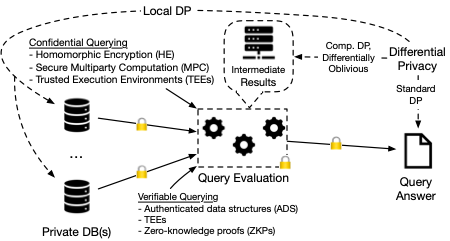
\includegraphics[bb = 0 0 220 118]{submissions/submission1/figs/pets-workflow.png}
        \caption{ Trustworthy DBs  in the query lifecycle}
    \label{fig:pets-workflow}
\end{wrapfigure}




\subsection{Query Lifecycle}

Figure~\ref{fig:pets-workflow} shows the broad steps with which a database system  evaluate a query and where they integrate assorted privacy and security-enhancing techniques into this workflow.  This figure is inspired by~\cite{secretflow2024survey}.  The dotted lines denote steps in the process that may leak information about a database's private records.  We expect  the initial input databases from one or more {\em data providers} or {\em data owners} are correct and complete at setup time.  A {\em clients} queries the records of one or more private databases.  The party computing the query answer\textendash this could be the data owner themselves, an untrusted cloud service provider used for outsourcing or others\textendash may have access to this information leakage.   We delve into specific trustworthy database architectures and the \sandp-preserving techniques that power them in the upcoming sections.    




\begin{figure}
\centering
    \subfloat[Client-Server]{
    \label{fig:arch:client-server}
    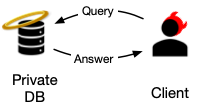
\includegraphics[bb= 0 0 113 65]{submissions/submission1/figs/client-server.png}}
    \hfill
    \subfloat[Outsourced Storage]{
    \label{fig:arch:outsourced-storage}
    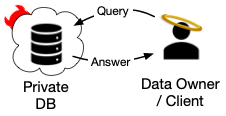
\includegraphics[bb= 0 0 113 65]{submissions/submission1/figs/outsourced-storage.png}}
    \hfill
    \subfloat[Private Data Federation]{
    \label{fig:arch:private-data-federation}
    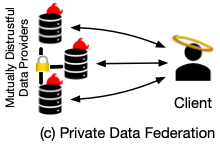
\includegraphics[bb= 0 0 113 65]{submissions/submission1/figs/private-data-federation.png}}  
    \hfill
    \subfloat[Outsourced  Computation]{
    \label{fig:arch:outsourced-computation}
    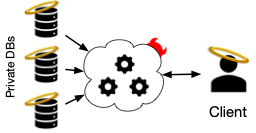
\includegraphics[bb= 0 0 113 65]{submissions/submission1/figs/outsourced-computation.png}}  
    \caption{Reference architectures for trustworthy database systems.}
    \label{fig:arch}
\end{figure}



\subsection{Trustworthy DBMS Architectures and Roadmap}
\label{sec:arch}

Throughout this text, we will reference several common architectures for query evaluation.  In this section, we will describe trustworthy database systems in terms of the  four architectures shown in Figure~\ref{fig:arch}. Our goal is to provide a  guide for future systems builders in selecting the most suitable one for their setting.  Admittedly, these frameworks are partially overlapping. We break them up as shown for ease of exposition.
 
A {\em client-server} architecture simply enables the client to send their  \query to the server with a private database and receive its answer, \answer as in Figure~\ref{fig:arch:client-server}.    For example, if the client is untrusted and the data provider is trusted, then the latter might protect their query answers from reconstruction by returning noisy versions of the true query answer using differential privacy.  We will cover this approach in Section~\ref{sec:dp}. 


The {\em outsourced storage} architecture, depicted in Figure~\ref{fig:arch:outsourced-storage}, starts with one or more untrusted cloud servers that have ample storage and limited compute resources. A data owner or trusted client outsources their storage operations to this platform to keep their data confidential.   These systems support a key-value store-esque interface. This is challenging because even when the database is stored encrypted, side-channel information such as memory access patterns can reveal some or all of the DB's contents~\cite{grubbs2016breaking,kellaris2016generic,markatou2019full}.  We introduce oblivious RAM in Section~\ref{sec:oram}; it is the main starting point for systems in this space.   If the client seeks only verifiable results, and they have access to more compute power on the server side,  they  might engage in verifiable querying as described in Section~\ref{sec:verifiable}.


The {\em private data federation} (PDF), shown in Figure~\ref{fig:arch:private-data-federation}, enables two or more mutually distrustful parties to compute \answer over the union of their private records without disclosing their private records to anyone.  This secure query evaluation may take place within cryptographic protocols evaluated among the data providers, described in Section~\ref{sec:oblivious} or in trusted hardware, as detailed in Section~\ref{sec:tees}.  


The {\em outsourced computation} setting in Figure~\ref{fig:arch:outsourced-computation} is when one or more data providers outsource their storage to the untrusted cloud and they delegate all query evaluation to this platform.  Here, the client and data providers are both trusted.  We discuss approaches to solving this challenge in Section~\ref{sec:secure}.  Similar to the PDF, platforms can securely compute in hardware or software.  This setup introduces another option: homomorphic encryption, or computing over encrypted data, as described in Section~\ref{sec:he}.

\section{Secure Query Processing}
\label{sec:secure}

In this section, we will examine techniques for query processing on outsourced databases, Figure~\ref{fig:arch:outsourced-computation}, and private data federations, Figure~\ref{fig:arch:private-data-federation}.   We group together these two architectures because there is strong overlap in their approaches and we highlight their differences we go along. We start with the strongest guarantee, oblivious querying, and then introduce popular relaxations to this. 

\subsection{Oblivious Querying}
\label{sec:oblivious}

A program is {\em oblivious} if its data access patterns and instruction traces are independent of their private input data.   \cut{An oblivious program's control flow does not change as a function of its private inputs.}  Oblivious algorithms prevent an attacker from inferring information about a database by observing its queries as they are evaluated.  An obliviously-executed query divulges nothing about its private inputs, except that which can be deduced from its results.

Researchers prove that a program is oblivious using the ``real world, ideal world'' paradigm~\cite{Canetti2001}.  Say that we are computing query  \query with mechanism \mechanism over database \db and there exists a probabilistic polynomial time simulator, $Sim$ that receives \db', an arbitrary database that is not \db but shares its schema and table cardinalities.   The observable traces of \mechanism should be computationally indistinguishable from those of $Sim$.  In other words, $Traces(\mathcal{M}, \mathcal{D}) \equiv Sim(\mathcal{M}, \mathcal{D}')$.  This paradigm makes it possible to compose independently developed building blocks, such as the oblivious query operators, into a query plan with strong end-to-end guarantees.  

There are a few common mechanics in oblivious database operators~\cite{bater2017smcql, zheng2017opaque,volgushev2019conclave,liagouris2023secrecy,ant2024scql}.  To keep their instruction traces oblivious to their private inputs, these programs evaluate both branches of private if-then statements, retaining only the one indicated by its secret conditional.  Similarly, they do not admit early termination of loops.  They conceal the selectivity of database operators with {\em dummy tuples} that replace rows that would be filtered out in an operator so that a curious observer cannot deduce anything  about a function's input data.  These engines typically represent this feature with a {\em dummy tag} or bit appended to each row  denoting whether it should be included in any subsequent calculations.  For example, an oblivious filter visits every row in a table and  applies its private predicate.   If the row satisfies the selection criteria, the oblivious if-then will update the row's dummy tag.  Otherwise,  it will simply overwrite the dummy tag with its previous value to remain oblivious.  We will describe oblivious database operators in detail in Section~\ref{sec:ops}.


Oblivious querying incurs a substantial performance penalty because its operators hide their data access patterns and any data-dependent changes in their control flow. With no additional info, queries with cascading joins must pad their output to the maximum possible size (the cross-product of their inputs) to conceal their selectivity.  Cumulatively, leads to a blow-up in their cardinalities increasing the cost of any subsequent computation.   As such, many oblivious database operators engage in selective information disclosure such as revealing the true cardinality of joins~\cite{krastnikov13efficient, zheng2017opaque} by default while offering full-padding  if desired.  If this is the root (last) operator in a query tree and the parties will receive \answer, then this is a sensible trade-off.  This picture gets more complicated if it is an intermediate result.


{\em Secure multiparty computation} (MPC)~\cite{goldreich1987mpc,lindell2021mpc} enables two or mutually distrustful parties to jointly compute over their private inputs obliviously.  Although early applied MPC protocols often implemented a special-purpose function (such as linear regression) to tackle the breathtaking overhead associated with general-purpose protocols, most modern systems compile their program logic into circuits~\cite{marcella2019sokmpccompilers}.  These {\em garbled circuits} reduce \query  into a series of gates, e.g., AND and XOR gates.  The protocol evaluates the circuit obliviously by traversing it in topological order.  They provide a Turing complete springboard for evaluating ad-hoc queries.   Some protocols use arithmetic gates instead of logic ones.   Performing all private computation within garbled circuits makes it possible to seamlessly compose the security guarantees of multiple, independently-developed components into a single proof under universal composability~\cite{Canetti2001}. 


\shortsection{Private Data Federations} There is a growing need to analyze information from multiple sources through a unified querying interface while addressing privacy concerns and complying with numerous privacy laws. A PDF, as  in Figure~\ref{fig:arch:private-data-federation}, integrates multiple autonomous database systems owned by mutually distrustful parties to query them as if they were a single query engine.  PDFs offer a shared schema that has table definitions agreed upon by all data providers at setup time.  It specifies the security level needed for each column.  Many PDF frameworks evaluate their queries under MPC.    This ensures that no unauthorized data is disclosed to other data providers participating in a secure query, while also minimizing the operations that \mechanism must perform under MPC by pushing them down for local evaluation~\cite{bater2017smcql, volgushev2019conclave, liagouris2023secrecy}.  


Data providers store private data in their own databases and compute query outputs in a privacy-preserving manner.  In PDFs, the process operates as follows: the client translates \query into the corresponding cryptographic protocols with which they will execute it.  They then send these instructions to all participating data providers.  The data providers then locally compute any public query operators  over their private records.  They then encode their selected private input rows for the operators that require secure, distributed evaluation over their unioned intermediate results.  They execute their oblivious operators by passing encrypted messages among themselves.  The data providers then send their share of \answer to the client over an encrypted link.  After receiving shares from all of the computing parties, the client assembles \answer. 

There are numerous threat models for MPC protocols, and they are detailed in~\cite{lindell2021mpc}.    A {\em semi-honest} party adheres to the protocols, but may attempt to learn additional, unauthorized information from observing the MPC protocol.  Semi-honest database systems include SMCQL~\cite{bater2017smcql}, Conclave~\cite{volgushev2019conclave}, and Hu-Fu~\cite{tong2022hu}. On the other hand, a {\em malicious} party both seeks to reveal information about a query's private inputs and they may deviate from the MPC protocol arbitrarily.  Senate~\cite{poddar2021senate} implements a PDF in the maliciously secure setting.  Some engines are starting to support multiple protocols or mixed models by compiling queries into abstract circuits (or methods) and applying different protocols for different settings.  SCQL~\cite{ant2024scql} and VaultDB~\cite{rogers2022vaultdb, vaultdb} take this approach.  Naturally, protocols with stronger guarantees incur more overhead for query evaluation, and this design choice depends on the setting in which they run.

\shortsection{Outsourced Computation}  MPC facilitates querying over the unioned data of 2+ independent private DBs.  We need one more step to extend this technology to the outsourced computation setting in Figure~\ref{fig:arch:outsourced-computation}.  To distribute trust over multiple outsourced hosts, a client may  {\em secret share} their private inputs and send shares of them to all computing parties.  Here no  party can reconstruct the secret unless the party colludes with a subset of parties. Before starting to evaluate \query's garbled circuits,  the parties participate in an {\em oblivious transfer} protocol to encode their data as wire labels for its logic gates.   This process is analogous to public-key cryptography where at the end of it each party holds an encrypted copy of the database without access to the key with which to decrypt it and none has access to the plaintext data except its initial owner.   


Platforms in the outsourced computation model have also been adopting MPC protocols.  The earliest work (to the best of our knowledge) in this space computed aggregates semi-honestly under 3-party computation~\cite{bogdanov2008sharemind}.  SDB~\cite{wong2014secure,Zhian2015SDB} created a hybrid model where the private data is secret-shared among the data owner and the cloud service provider.  For the semi-honest setting, Secrecy~\cite{liagouris2023secrecy} supports 3-party secure computation over ad-hoc SQL queries.     RESCU-SQL~\cite{li2023rescu} uses maliciously secure, $n$-party MPC protocols to protect outsourced data in the zero-trust cloud.  




\subsection{Oblivious RAM for Outsourced Storage}
\label{sec:oram}

We now turn our attention to the outsourced storage setting shown in Figure~\ref{fig:arch:outsourced-storage} in Section~\ref{sec:arch}.  Here, the client wishes to outsource the of their private database to the untrusted cloud.  If they simply encrypted their data and issued read and write requests against the specific records as they access them, then this will expose their data access patterns and make their data vulnerable to side-channel leakage attacks~\cite{kellaris2016generic, naveed2015inference, grubbs2016breaking}.  Unless otherwise specified, these systems have a key-value store-style API.   {\em Oblivious RAM}~\cite{goldreich1987oram} transforms a client's read and write requests into ones that are independent of their true memory access patterns. When a client requests a block, $b_i$, from their database, the ORAM rewrites it as a series of reads and writes that 1) shuffle their storage, and 2) pad their request with dummies to conceal the position of their request in the database.    This makes the distribution of their I/O requests oblivious to their true memory access patterns.  It also prevents an adversary from deducing the frequency of accesses to a specific $b_i$.  

Early work in outsourced storage centered on ORAM constructions themselves, with tree-based ones~\cite{stefanov2013pathoram, ren2015constants} emerging as the dominant paradigm in practice.  Several systems have generalized this work to distributed ORAMs, including Shroud~\cite{lorch2013shroud}, ObliviStore~\cite{stefanov2013oblivistore}, and TaoStore~\cite{sahin2016taostore}.  Snoopy~\cite{dauterman2021snoopy} integrates trusted hardware into their design to parallelize oblivious reads and writes.   Whereas ORAM makes all access requests indistinguishable from one another,  {\em frequency smoothing} relaxes this requirement to make the frequency with which individual $b_i$s are requested uniform.  Waffle~\cite{maiyya2023waffle} and Pancake~\cite{grubbs2020pancake} are examples of this approach. They do so by replicating popular objects and padding their I/O requests with dummies. 


The systems described above are all linearizable; they reason about concurrency at the granularity of one object at a time.  Additional mechanisms are needed for ACID transactions.   Obladi~\cite{crooks2018obladi} is an ORAM-backed storage engine that parallelizes ACID transactions on untrusted ORAM servers.  Treaty~\cite{giantsidi2022treaty} is a natural extension of this work obviates the need for a trusted proxy with trusted hardware.


\subsection{Homomorphic Encryption for Outsourced Computation}
\label{sec:he}

{\it Homomorphic encryption} (HE)~\cite{gentry2009fully} enables a system to compute over encrypted data without decrypting it.    HE and MPC are close cryptographic cousins.  Rather than distributing trust over multiple parties, HE enables data owners to outsource their operations to one host with a variation of the outsourced computation architecture in Figure~\ref{fig:arch}.  Here, the data provider encrypts their records and uploads them to the untrusted cloud (without providing the decryption key) and the client issues queries against the encrypted databases.   Whereas MPC enables parties to pipeline their circuit evaluation, i.e., compute each gate and discard intermediate wire labels when they are no longer needed, HE protocols evaluate a materialized circuit to produce \answer and send it to the client.  This is more efficient for straightforward operators such as filter, but may reveal scalability challenges for ones with deeper circuits such as aggregating over a large group of tuples.  Fully homomorphic encryption (FHE)  support circuits, and thus ad-hoc queries, without leaking information about the encrypted data.  FHE has a very high performance cost, typically several orders of magnitude slower than running in plaintext.  These schemes have seen limited adoption in databases in practice with the only known implementation for databases targeting aggregation alone~\cite{ren2022heda}.  HE has several relaxations to bridge this performance gap.  Some partially homomorphic encryption (PHE) schemes offer better performance in exchange for reduced security guarantees, such as order preserving encryption~\cite{boldyreva2009order,agrawal2004order} and deterministic encryption~\cite{boldyreva2008notions, bellare2008deterministic}.  Others support reduced expressiveness with higher performance, such as additive HE~\cite{paillier1999public} and multiplicative HE~\cite{elgamal1985public,rivest1978method}.

Database researchers have invested substantial research effort into bringing these encryption schemes to outsourced databases with a variation of the architecture in Figure~\ref{fig:arch:outsourced-computation}.  The data owner encrypts \db using HE and uploads them to the untrusted cloud server.  The client submits \query to the server and it computes \answer over its encrypted copy of \db.  ~\cite{agrawal2004order} introduced order-preserving encryption for answering database queries.  CryptDB~\cite{popa2011cryptdb}
and Monomi~\cite{tu2013processing} targeted HE for outsourced databases for OLTP and OLAP workloads, respectively.  The latter identified lightweight mechanisms for moving some of the query evaluation client-side to circumvent the performance limitations of FHE.  Unfortunately, these PHE schemes have substantial side-channel leakage associated with executing queries over them~\cite{naveed2015inference, bindschaedler2017tao}.  This is similar to the issues we described for non-oblivious access to outsourced storage above.  SEAL~\cite{demertzis2020seal} tackles some of this leakage with adjustable leakage that hides $\binom{n}{k}$ bits out of a search key by introducing a generalization of ORAM.


\subsection{Trusted Execution Environments for Outsourced and Federated Querying} 
\label{sec:tees}

Trusted Execution Environments, or TEEs, create an isolated computing platform within an untrusted computer using trusted hardware.  They have encrypted private memory with which they runs sealed code that is confirmed to be only the code given by the client or a proxy thereof (such as a trustworthy DBMS).  Hence, code run within TEEs are verifiable by virtue of running within a secure enclave, such as Intel SGX~\cite{dinh2019everything} and ARM TrustZone~\cite{pinto2019demystifying}.   Clients  delegate their program executions to trusted hardware, safeguarding their private data without the need for encryption. The main advantage is its efficiency, as it avoids the significant computational and communication overhead typically incurred by cryptographic primitives, making it more practical for real-world scenarios. Secure enclaves alone are not a panacea. For example, instruction traces leak memory access patterns, allowing eavesdroppers to infer private data from them~\cite{kellaris2016generic,markatou2019full}.

TEEs are seeing increased use for evaluating queries over confidential data  the cloud or outsourced computation in Figure~\ref{fig:arch:outsourced-computation}.  First-generation systems relied on software-hardware co-design to build TEEs with bespoke algorithms for query evaluation such as TrustedDB~\cite{bajaj2011trusteddb} from IBM and Microsoft's Cipherbase~\cite{arasu2013orthogonal}.  As SGX and other enclaves became widely available and cloud-ready, researchers created secure enclave extensions to well-known DBMSs.  For example, StealthDB~\cite{vinayagamurthy2019stealthdb} builds atop PostgreSQL and EnclaveDB~\cite{priebe2018enclavedb} runs within Hekaton.  In addition, since the resident host running the enclave can observe its memory access patterns, researchers have been building oblivious algorithms for use inside the TEE such as ObliDB~\cite{eskandarian2019oblidb} and Opaque~\cite{zheng2017opaque}.  This approach has also been appearing in TEE-based PDFs such as~\cite{dave2020oblivious}. 





\section{Differential Privacy} 
\label{sec:dp}

If the client is untrusted, the data provider may call for guarantees that prevent them from using query answers to infer information about their private input records. Speaking informally, {\em Differential Privacy} (DP) ~\cite{dp2006, dwork2008differential} protects private data from construction attacks by injecting carefully calibrated noise into their query answers to control their resulting information leakage before returning them to the client.   An algorithm satisfies differential privacy if its output is approximately the same over a database, \db, as it would be over a neighboring database differing by one record, \db'. This workflow, of a data provider or trusted curator noising query answers before releasing them to the client, is known as {\em Standard DP} or SDP~\cite{wagh2021dp}.     More broadly, if a secure database reveals precise, un-noised query answers, this creates unbounded information leakage~\cite{kifer2011no}.  SDP works on the client-server model in Figure~\ref{fig:arch:client-server}. 

Before answering their first query over \db, the data owner selects a privacy budget, \eps, with which they limit the information they leak in aggregate to the client or clients by answering their queries.  Recall that $\mathcal{R} := \mathcal{M}(\mathcal{D})$.   In its simplest form, if the client queries a private database $n$ times with mechanisms $\mathcal{M}_1, \ldots, \mathcal{M}_n$, and $\mathcal{M}_i$ has $\epsilon_i$, their net privacy loss is $\sum_{i=1}^n \epsilon_i$.  Researchers have proposed several frameworks for designing efficient DP mechanisms~\cite{johnson2020chorus, zhang2018ektelo, wang2021dpgen}.  Also, the database community has invested significant research effort into automatically deriving SDP answers to SQL queries with robust e2e  privacy guarantees ~\cite{ann2011airavat,mcsherry2009privacy,proserpio2014calibrating,johnson2018towards,kotsogiannis2019architecting, kotsogiannis2019privatesql}.



Choosing \eps for a given database and query workload reveals a trade-off between utility and privacy.  A larger \eps means that \mechanism will inject less noise into \answer.  In other words, more accurate query answers result in a greater privacy loss for \db.   Selecting an \eps with sufficient data protection while producing useful query answers is a challenging topic~\cite{lee2011much} and the subject of ongoing research~\cite{dwork2019differential, li2023towards, near2023guidelines}.  A conservative heuristic is to restrict $\epsilon$ to values less than or equal to one~\cite{wood2018differential}.

\subsection{Computational Differential Privacy} One major shortcoming of SDP is that assumes there is a single trusted data curator noising \answer.   \cut{It is attractive because its guarantees are information-theoretic.}  Computational DP (CDP)~\cite{beimel2008distributed, mironov2009computational} relaxes SDP's strong information-theoretic guarantees to a weaker, probabilistic polynomial time adversary in exchange for less noisy results and support for distributed data.   CDP quantifies information leakage when two or more parties are computing a function over their encrypted and unioned private inputs, $\mathcal{D}_*$.    It frames information leakage about \mechanism's intermediate results as a differentially private view of $\mathcal{D}_*$ and assigns some share of the privacy budget to it.    For example, if we are computing a CDP filter $\mathcal{R} := \sigma(\mathcal{D})$ we may start by running the oblivious evaluation described above.   We then generate a noisy version of its true output cardinality {\em within} the oblivious algorithm for release, $|\widetilde{\mathcal{R}}|$ and obliviously delete dummy rows.  This will make any parent operators run faster because they compute over fewer dummies. 

CDP introduces a third dimension to our DP trade-off:  performance.
If we allocate more privacy to computation, the client may get their query answer faster but with reduced accuracy because we spend some privacy releasing information about \mechanism's intermediate results, i.e., its noisy intermediate cardinality.  There's been significant research interest in using CDP to accelerate privacy-preserving query evaluation in PDFs~\cite{bater2018shrinkwrap, bater2020saqe,he2017composing}. 


CDP  extends to the outsourced storage setting.  Allowing an untrusted cloud service provider to view noisy versions of the client's memory access patterns enables this trade-off on efficiency and privacy.   DP-ORAM~\cite{wagh2018differentially} relaxes ORAM's full-oblivious guarantees to CDP ones.    $\epsilon$psolute~\cite{kellaris2017accessing, bogatov2021varepsilonpsolute} parallelizes CDP I/O requests among multiple ORAMs.   CDP has also been used to speed up outsourced computation for analytics~\cite{roy2020cryptepsilon} and for querying growing databases~\cite{zhang2023longshot, wang2022incshrink,wang2021dp} in the untrusted cloud.  



\subsection{Differential Obliviousness}
 Another DP relaxation gaining traction in the database community is differential obliviousness~\cite{chan2022foundations,chu2021differentially, qin2022adore, qiu2023doquet} (DO).   A DO algorithm offers a DP view of its memory traces by leaking approximate versions thereof.   This is related to CDP, with the latter approximating discrete views of \db.  To continue with our filter running example, a simplified version of the DO filter in~\cite{qin2022adore} partitions \db into batches of length $B$ where $B$ is polylog of $|$\db$|$. In lieu of running an oblivious filter, it writes to the output buffer of \answer one batch at a time maintaining a cursor for these writes.  For each block $b_i$ it computes a DP approximation of its prefix sum (how many rows are selected), this provides a range of the count of the rows $b_i$ will emit to \answer.  It then writes to $B$ slots in the output buffer with a mix of real and dummy rows and advances the cursor to the position indicated by the lower bound of its DP prefix sum. 
 
 DO strikes a balance between full-oblivious ones and ones with unbounded information leakage.   It admits secure algorithms with performance properties comparable to streaming or pipelined operators and it boasts better cache efficiency than approaches that materialize their entire \answer before noising it.     On the other hand, DO mechanisms are non-trivial compose~\cite{zhou2023theory}, and they need to maintain the notion of neighbor-preserving differentially oblivious datasets between an operator's input and output relations to compose a DAG of them.  Addressing this challenge is a topic of ongoing research.

\subsection{Local Differential Privacy}

  One more approach to limiting information leakage from querying private data is injecting noise into the private data before querying it.  Local DP~\cite{xiong2020comprehensive} (LDP) removes the need for a trusted data curator by noising it one row at a time.  There has been considerable research in incorporating this into database operations~\cite{cormode2018privacy,gu2019supporting,roth2020orchard,wang2017locally,xu13collecting}.  This is different from DP synthetic data generation~\cite{cai2023privlava,ge2021kamino,machanavajjhala2008privacy}, which creates a new dataset with values that mimic the distribution of a private one.  


LDP is attractive for aggregating ``wisdom of the crowd'' statistics, such as collecting new words and phrases for auto-complete as they enter the popular lexicon and identifying software bugs from noisy bug reports.  It also frees data collectors from the liability of storing raw user data, which may garner subpoenas or attempts to steal it.  Also, since the data are noised upfront,  clients may query it as many times as they wish without eroding the privacy budget.  On the other hand, because the data are perturbed one row at a time, the algorithm needs to add $O(\sqrt{n})$ to each entry for $n$ individuals contributing to \db, whereas SDP would simply noise the true count independent of the participant count~\cite{wagh2021dp}.




\section{Verifiable Querying}
\label{sec:verifiable}

Data owners are increasingly outsourcing their data management to the untrusted cloud.   With {\em verifiable computing} when an untrusted server answers a client query \query with \answer over a private database \db, they participate in a protocol to convince the client (with high probability) that \answer is correct and complete.   Here we have two participants: a prover \prover, the cloud service provider, and a verifier \verifier, the client.   If $\mathcal{C}_{ver}(\mathcal{D})$ is a function with which \prover and \verifier authenticates $\mathcal{R}$ with the following guarantees:
\vspace{-0.2cm}
\begin{itemize}
    \item Completeness.  If \prover faithfully executes \query then $ \mathcal{C}_{ver}(\mathcal{R})=1$.  \prover accepts honest proofs.
    \vspace{-0.3cm}
    \item Soundness.  If \prover outputs an incorrect \answer,  $Pr[\mathcal{C}_{ver}(\mathcal{R})=1] \leq \epsilon$, where $\epsilon$ is a negligible probability.
\end{itemize}
\vspace{-0.2cm}
Systems such as IntegriDB~\cite{zhang2015integridb}, Concerto~\cite{arasu2017concerto}, CorrectDB~\cite{bajaj2013correctdb}, VeriDB~\cite{zhou2021veridb} and vSQL~\cite{zhang2017vsql} use VC to guarantee data integrity for querying.  


There are several approaches to creating verifiable query answers.  With an {\em Authenticated Data Structure}, \prover generates a proof that accompanies \answer to validate that it is complete and sound.  The two main methods that instantiate ADS are tree-based and signature-based methods.  The tree-based method builds a binary tree for a database, where each leaf node stores a digest about tuples in the database, and its internal nodes are digests that summarize its children.   When evaluating a query, the database sends the query answer along with a set of digests for the relevant nodes to the client, who has the digest of the root node, to verify the answer by reconstructing the path to match the root node. IntegriDB is such a system that applies a dynamic tree-based ADS tailored for a specific set of queries, allowing the client to query and verify $\mathcal{R}$ using precomputed digests aided by the accompanying proof. On the other hand, signature-based methods constructs a set of signatures for tuples in the database. During query evaluation, the cloud-hosted database sequentially collects a set of signed tuples that it accesses. Then the client verifies each tuple that no unwanted tuple is included and no necessary tuple is missed.

Similarly, Concerto, CorrectDB and VeriDB utilize ADS-based verifiable computing to verify their queries, but they compose ADSs with TEEs benefit from greater efficiency than working solely with cryptographic primitives (see Section~\ref{sec:tees}). Concerto is a concurrent key-value store, while VeriDB and CorrectDB support ad-hoc SQL queries for relational databases.

With {\em interactive proofs}~\cite{zhang2015integridb}, \prover and \verifier  work together to confirm the authenticity of  a statement $C(w)$ over a witness $w$ via multiple rounds of challenge-response messages, thereby incrementally ensuring correctness and soundness.  This VC approach is an alternative to ADS.  Similar to MPC, these proofs work in the circuit paradigm\textendash they express their logic as gates. In our context, $w$ is the private database $\mathcal{D}$.  \prover and \verifier interactively establish $w$ as a commitment of \db.  This forms the immutable starting point for \prover's proof for \query. Upon receiving the last respone $\mathcal{R}$ from \prover, \verifier accepts it iif $\mathcal{C}_{ver}(\mathcal{R})=1$. In other words, \verifier rejects immediately if it receives any unconvincing response from \prover during the interaction. In contrast to ADS-based systems mentioned above, vSQL is more expressive by supporting a wider range of SQL queries through IPs. Although interactive proofs incur significant communication overhead between the client and server, vSQL operates with nearly the same efficiency as those systems.

However, the client might attempt to obtain extra information that it is not authorized to access. For example, VC-backed systems with ADS and interactive proofs ensure the integrity of an outsourced database, but they reveal the data owner's records to the cloud service provider. Moreover, TEE-based systems may leak memory access patterns through program traces, as discussed in Section~\ref{sec:tees}. Therefore, the aforementioned systems are inadequate to protect private data on an untrusted server. For this we need to add one more guarantee to our stack, {\em zero knowledge}~\cite{goldreich1991zkp,goldwasser1985zkp}:
\vspace{-0.2cm}
\begin{itemize}
    \item Zero knowledge. If  $\mathcal{C}_{ver}(\mathcal{R})=1$, \verifier learns nothing other than the fact \answer was computed correctly.
\end{itemize}
\vspace{-0.2cm}
To provide such a stronger guarantee in verifiable querying, the database community has adopted {\it zero-knowledge proofs} for SQL queries~\cite{zhang2017vsqlzk, li2023zksql} to offer privacy and confidentiality for query answering.  This guarantee is similar to the one we saw for obliviousness: \verifier learns nothing more than \answer and that which can be deduced from it.  The main difference here is that \prover is able to prove  properties of intermediate query results, such as proving a sorted list of tuples is monotonically increasing, rather than evaluating the entire program logic in circuits. Overall, \zkps enable \prover to convince \verifier of the query answer \answer by authenticating it with a proof, without revealing any additional information beyond the information that could be derived from \answer. This means we could simultaneously address both data integrity and data privacy for the outsourced database.



There are two main flavors of zero-knowledge proofs: {\it interactive} and {\it non-interactive} \zkps.  Interactive ones are analogous to MPC, where \prover and \verifier verify a circuit one gate at a time using pipelined gates. In contrast to IPs, \zkps divulges no additional information about $w$ beside the truth of $C(w)$ to \verifier while IPs do not hide $w$ from \verifier.

Zero-knowledge extension of vSQL~\cite{zhang2017vsqlzk} and ZKSQL~\cite{li2023zksql} utilize interactive \zkps. While the former remains theoretical as a pioneering effort, ZKSQL optimizes computationally expensive operators for practical use, such as sort and join, reducing their respective complexities from $O(n \log n)$ and $O(n^2)$ to $O(n)$. This optimization is achieved through \prover's local computation and interactive verification with ZK set operations, where the set-based proofs are represented by polynomials instead of circuits, unlike conventional interactive \zkps. For example, in sorting, we can only check if the result contains the same tuples as the unsorted table using ZK set equality when the result confirms to be monotonically increasing or decreasing.

Conversely, non-interactive ones construct a monolithic circuit for their query in a single step, providing a single proof that \prover sends with \answer. They require no additional interaction between \prover and \verifier and are widely used in blockchain applications. However, a significant drawback is the large proof size, which can be memory-intensive due to the one-shot construction. Despite potentially being more efficient than the interactive ones due to reduced communication overhead, we do not recommend this approach for systems aiming to scalability.

In addition to the single prover-verifier system, there are also distributed or decentralized verification systems that build atop blockchains~\cite{el2019blockchaindb, allen2019veritas, peng2020falcondb,yueglassdb}. They guarantee auditability, accountability, and traceability on the ledger during data sharing across mutually distrustful parties, but their combined records are largely accessible to all participants on the chain thus they are beyond the scope of this paper.

\section{Privacy-Preserving Database Operators}
\label{sec:ops}

This section introduces privacy-preserving database operators.  They are crucial for secure and privacy-preserving query evaluation. 


We start with oblivious operators.  Recall from Section~\ref{sec:oblivious} that they guarantee that their memory access patterns and program traces do not disclose any information about their private inputs.   These operators ensure that even if an adversary knows \query and observes its execution under \mechanism, they learn no additional information from participating in its evaluation.~\cite{arasu2014oblivious} introduced the earliest formal definitions for efficient algorithms for oblivious query processing.  This paper covers approaches for selections, joins, and group-by aggregation.  It was designed for use in TEEs, although no practical implementation of its results are forthcoming.  Since then, there has been a lot of excitement in the research community about creating efficient, oblivious algorithms for database operators~\cite{ant2024scql, bater2017smcql, krastnikov13efficient, zheng2017opaque}.  We will also touch upon operators that offer alternative privacy guarantees, such as CDP and DO from Section~\ref{sec:dp}.  We will mainly focus on joins in this survey because, in our experience, these tend to be the bottleneck for most secure query workloads.  In addition, joins have attracted the most research results to date in terms of operator algorithms proposed.

\subsection{Joins}

Table~\ref{tbl:joins} presents a comprehensive categorization of privacy-preserving join approaches. This considers several key dimensions: computational complexity, employed methods, type of leakage, number of participating parties, and supporting join types. Notably, the table organizes the joins based on their leakage, establishing distinct categories for oblivious joins, differentially oblivious joins, and differentially private joins. 


\begin{table}
    \centering
    \begin{tabular}{l|c|c|c|p{2.8cm}|c}
     {\bf Strategy}    & {\bf Complexity} &{\bf  Compute Method} & {\bf Leakage}  &{\bf  \# of Parties} & {\bf Join Type} \\
     \hline 
     Nested Loop & $O(n^2)$ & SH-2PC & Oblivious & 2:~\cite{bater2017smcql, vaultdb} & all \\
     
      &  &  SH-3PC & Oblivious  &  3:~\cite{volgushev2019conclave, liagouris2023secrecy} &  \\

      &  &  Mal-MPC & Oblivious  &  N:~\cite{li2023rescu} &  \\
     
      &  &  SH-2PC &   CDP &  2:~\cite{bater2018shrinkwrap, bater2020saqe} &  \\
       &  & TEE & Oblivious &  1:~\cite{li2008privacy}, $\geq2$:~\cite{dave2020oblivious}&  \\
       
     \hline
     NLJ w/semi-join & $(n \times RF)^2$ & SH-2PC & Oblivious & 2:  \cite{bater2017smcql}  & equi-join \\ 
    &  &SH-3PC  &  Oblivious  &  3:~\cite{chu2021differentially, liagouris2023secrecy} & \\ 
     \hline

    Index NLJ & $n \log ^2 n$ & ORAM & Oblivious & N:  \cite{chang2022towards}  & all \\ 
    \hline

    Sort-Merge Join & $n \log ^2 n$ & TEE & Oblivious & $\geq 1$: \cite{krastnikov13efficient, eskandarian2019oblidb, zheng2017opaque} & equi-join \\ 
                    &    & SH-3PC & Oblivious & 3:~\cite{li2024experimental} & \\
                    &    & TEE & DO & $\geq 1:$  \cite{chu2021differentially}& \\
                    \hline 
       PK-FK SMJ             & $n \log n$   & TEE & DO & $\geq 1$:~\cite{qin2022adore} & 1:n \\
     \hline
    
     Hash Join & $n$ & SH-3PC & Oblivious& 3:~\cite{mohassel2020fast} & equi-join \\ 
     \hline

     Hash SMJ & $n$ & SH-3PC & Oblivious& 3:~\cite{luo2024secure} & equi-join \\ 
     \hline

     PSI join & $n$ & SH-2PC & Oblivious & 2:~\cite{raghuraman2022blazing, wang2021secure}; & pk-pk \\
      & & Mal-2PC & Oblivious & 2:~\cite{raghuraman2022blazing} & pk-pk \\
      & $n \log n$  & SH-MPC & Oblivious & N:~\cite{ant2024scql} & equi-join \\
      & $n \ln \ln n$  & SH-MPC & CDP & N:~\cite{narayan2012djoin} & equi-join \\
      \hline
      
      Partition Join & $n \log ^2 n$   & TEE & Oblivious & N:~\cite{li2023soda} & equi-join \\
      & $n \log n$   & TEE & DO & $\geq 1$:~\cite{qiu2023doquet} & equi-join \\
    \end{tabular}
    \caption{Comparison of secure join algorithms.   }
    \label{tbl:joins}
\end{table}


\shortsection{Oblivious Join}
The most strict technique is fully oblivious join, which allows combining data from different sources without revealing sensitive information. Various algorithms have been evaluated in~\cite{li2024experimental} to determine their efficiency and security, as shown in table~\ref{tbl:joins}. The study reveals the overall efficiency ranking, wherein PSI emerges as the most efficient, followed by hash approaches. However, the efficiency of NLJ and SMJ can surpass others under high join selectivity. Additionally, optimal join order significantly improves efficiency, highlighting the importance of cost-based query optimization. 

\shortsection{DO Joins}
To improve efficiency, DO join permits a controlled degree of information leakage about the data while still providing meaningful privacy guarantees based on the relaxed notion of $(\epsilon, \delta)-$differential obliviousness. Key advancements in this area include the DO join~\cite{chu2021differentially}, Adore~\cite{qin2022adore}, Doquet~\cite{qiu2023doquet}, as shown in Table~\ref{tbl:joins}. Fully oblivious join algorithms are inefficient due to worst-case padding, resulting in significant performance overheads. The DO join algorithm addresses this by using $(\epsilon, \delta)-$DO~\cite{chan2022foundations}, a less strict privacy concept, to achieve efficient joins compared to insecure methods while preserving privacy. This approach provides meaningful privacy guarantees and proves new lower bounds on DO join algorithm performance. Adore employs a similar strategy with a sort-merge join but improves efficiency by using bucket oblivious sort, reducing the sorting complexity from bitonic sort's O($n \log^2(n)$) to O($n \log n)$. Additionally, Doquet optimizes join costs through a partitioning approach, significantly improving performance. 


\shortsection{CDP Joins} CDP joins provide strong privacy guarantees by ensuring that the inclusion or exclusion of any individual in the dataset trivializes the join operation's outcome. DJoin~\cite{narayan2012djoin} supports SQL-style join queries across multiple databases using two novel primitives: Blinded, Noised Private Set Intersection Cardinality (BN-PSI-CA) for private intersections with added noise to ensure differential privacy, and Denoise-Combine-Renoise (DCR) which combines noised subset sizes efficiently for privacy-preserving joins on distributed data. This results in an efficient join complexity. Shrinkwrap~\cite{bater2018shrinkwrap} addresses inefficiencies in PDF by leveraging computation differential privacy to reduce intermediate result padding. It integrates a cost model and privacy budge optimizer to balance privacy and performance. SAQE~\cite{bater2020saqe} scales PDF to handle large datasets by combining DP with approximate query processing. It introduces secure sampling algorithm that reduce computation costs and minimize the noise injected into query results.  


\subsection{Additional Operators}

We will now focus on additional operators and frameworks in the trustworthy database system landscape.

\shortsection{Oblivious Aggregate}
Oblivious aggregation computes summary statistics over a set of records without revealing how they are partitioned with a {\tt GROUP BY} clause. {\sc SAGMA}~\cite{hackenjos2020sagma} and {\sc OBSCURE}~\cite{gupta12obscure} represent two approaches to this challenge. {\sc SAGMA} supports secure aggregation grouped by multiple attributes under somewhat holomorphic encryption (SWHE). It allows the user to choose any combination of grouping attributes and privately maps rows to buckets, balancing storage and computational needs. However, {\sc SAGMA}'s main drawback is its need to store an exponentially growing set of monomials because its SWHE encoding supports only one multiplication operation~\cite{ren2022heda}. On the other hand, {\sc OBSCURE} encodes private rows using order-preserving secret sharing (OP-SS), which maintains data order securely while supporting repeated aggregation queries. {\sc OBSCURE} also introduces an oblivious result verification mechanism and demonstrates scalability to large datasets, addressing challenges faced by previous secret-sharing or MPC systems. However, {\sc OBSCURE}'s use of OP-SS is not inherently secure and is vulnerable to background knowledge attacks. 

\shortsection{Oblivious Filter}
 QFilter~\cite{mirabi2023qfilter} combines an Attribute-Based Access Control (ABAC) model with query processing over secret-shared data. This integration allows for fine-grained access control while preserving privacy. It handles aggregation SQL queries like ``count", ``sum", and ``avg", without requiring inter-server communication, thus securing against honest-but-curious adversaries. The system efficiently handles queries through string matching-based operators, rewriting SQL queries to embed access authorizations and filter unauthorized data during execution. However, QFilter's limitations include its inability to support more complex queries like ``min" and ``max" functions, ``group-by" clauses, or range queries, which limits its applicability in demanding data environments.

\shortsection{SODA}
SODA~\cite{li2023soda} introduces a collection of oblivious algorithms designed for distributed data analytics, including filter, aggregate, and binary equi-join operations. It improves upon previous systems like Opaque~\cite{zheng2017opaque} by minimizing data padding through a two-level bin-packing strategy. This approach effectively manages input redistribution and handles join product skewness. SODA further avoids expensive global sort primitives by employing low-cost pseudo-random communication to guarantee uniform data traffic. However, SODA does not address issues related to denial-of-service attacks or physical side-channel attacks. Additionally, it does not integrate hardware oblivious memory, which could further protect against side-channel vulnerabilities by hiding access patterns more effectively.

\shortsection{Differentially Oblivious Operators}
 Adore~\cite{qin2022adore} not only achieves differential obliviousness for joins, but it extends this guarantee to other database operators, like selection and aggregation, by working within secure enclaves. Doquet~\cite{qiu2023doquet} introduces a framework for DO range and join queries using private data structures.  It improves on the efficiency of Adore and oblivious algorithms on SGX.   Doquet also addresses access pattern leakage vulnerabilities that were present in Adore, ensuring a more secure implementation than that of its predecessor.   Both systems highlight the potential of DO to trade off on privacy and efficiency in query evaluation.


\section{Conclusions}
\label{sec:conclusion}

In this paper we surveyed the state-of-the art in security and privacy-preserving database systems.  We compared the properties of competing frameworks for trustworthy querying, such as secure computation vs trusted hardware for secure querying and authenticated data structures vs interactive proving for verifiable querying.  In addition, we described how differential privacy is making its way into nearly all of the steps in the query lifecycle.  We highlighted how composing these techniques reveals many subtleties in their \sandp guarantees, such as computational differential privacy over secure computation.  We closed with an exploration of how these techniques come together to create efficient, privacy-preserving database operators.

\begin{thebibliography}{140}
\itemsep=1pt
\begin{small}

\bibitem{agrawal2004order}
R.~Agrawal, J.~Kiernan, R.~Srikant, and Y.~Xu.
\newblock Order preserving encryption for numeric data.
\newblock In {\em Proceedings of the 2004 ACM SIGMOD international conference
  on Management of data}, pages 563--574, 2004.

\bibitem{allen2019veritas}
L.~Allen, P.~Antonopoulos, A.~Arasu, J.~Gehrke, J.~Hammer, J.~Hunter,
  R.~Kaushik, D.~Kossmann, J.~Lee, and e.~a. Ravi~Ramamurthy.
\newblock Veritas: Shared verifiable databases and tables in the cloud.
\newblock In {\em 9th Biennial Conference on Innovative Data Systems Research
  (CIDR)}, pages 1--9, 2019.

\bibitem{secretflow2024survey}
{Ant Group}.
\newblock A comprehensive comparison of various privacy-preserving
  technologies.
\newblock \url{https://www.yuque.com/secret-flow/admin/exgixt72drdvdsy3}.
\newblock Accessed: 2024-06-12.

\bibitem{ant2024scql}
{Ant Group}.
\newblock Secure collaborative query language.
\newblock \url{https://github.com/secretflow/scql}.
\newblock Accessed: 2024-06-13.

\bibitem{arasu2013orthogonal}
A.~Arasu, S.~Blanas, K.~Eguro, R.~Kaushik, D.~Kossmann, R.~Ramamurthy, and
  R.~Venkatesan.
\newblock Orthogonal security with cipherbase.
\newblock In {\em CIDR}, 2013.

\bibitem{arasu2017concerto}
A.~Arasu, K.~Eguro, R.~Kaushik, D.~Kossmann, P.~Meng, V.~Pandey, and
  R.~Ramamurthy.
\newblock Concerto: A high concurrency key-value store with integrity.
\newblock In {\em Proceedings of the 2017 ACM International Conference on
  Management of Data}, pages 251--266, 2017.

\bibitem{arasu2014oblivious}
A.~Arasu and R.~Kaushik.
\newblock Oblivious query processing.
\newblock {\em ICDT}, 2014.

\bibitem{bajaj2011trusteddb}
S.~Bajaj and R.~Sion.
\newblock Trusteddb: a trusted hardware based database with privacy and data
  confidentiality.
\newblock In {\em Proceedings of the 2011 ACM SIGMOD International Conference
  on Management of data}, pages 205--216, 2011.

\bibitem{bajaj2013correctdb}
S.~Bajaj and R.~Sion.
\newblock Correctdb: Sql engine with practical query authentication.
\newblock {\em Proceedings of the VLDB Endowment}, 6(7):529--540, 2013.

\bibitem{bater2017smcql}
J.~Bater, G.~Elliott, C.~Eggen, S.~Goel, A.~N. Kho, and J.~Rogers.
\newblock Smcql: Secure query processing for private data networks.
\newblock {\em Proc. VLDB Endow.}, 10(6):673--684, 2017.

\bibitem{bater2018shrinkwrap}
J.~Bater, X.~He, W.~Ehrich, A.~Machanavajjhala, and J.~Rogers.
\newblock Shrinkwrap: efficient sql query processing in differentially private
  data federations.
\newblock {\em Proceedings of the VLDB Endowment}, 12(3), 2018.

\bibitem{bater2020saqe}
J.~Bater, Y.~Park, X.~He, X.~Wang, and J.~Rogers.
\newblock {SAQE}: practical privacy-preserving approximate query processing for
  data federations.
\newblock {\em Proceedings of the VLDB Endowment}, 13(12):2691--2705, 2020.

\bibitem{beimel2008distributed}
A.~Beimel, K.~Nissim, and E.~Omri.
\newblock Distributed private data analysis: Simultaneously solving how and
  what.
\newblock In {\em Advances in Cryptology--CRYPTO 2008: 28th Annual
  International Cryptology Conference, Santa Barbara, CA, USA, August 17-21,
  2008. Proceedings 28}, pages 451--468. Springer, 2008.

\bibitem{bellare2008deterministic}
M.~Bellare, M.~Fischlin, A.~O’Neill, and T.~Ristenpart.
\newblock Deterministic encryption: Definitional equivalences and constructions
  without random oracles.
\newblock In {\em Advances in Cryptology--CRYPTO 2008: 28th Annual
  International Cryptology Conference, Santa Barbara, CA, USA, August 17-21,
  2008. Proceedings 28}, pages 360--378. Springer, 2008.

\bibitem{bindschaedler2017tao}
V.~Bindschaedler, P.~Grubbs, D.~Cash, T.~Ristenpart, and V.~Shmatikov.
\newblock The tao of inference in privacy-protected databases.
\newblock {\em Cryptology ePrint Archive}, 2017.

\bibitem{bogatov2021varepsilonpsolute}
D.~Bogatov, G.~Kellaris, G.~Kollios, K.~Nissim, and A.~O'Neill.
\newblock \ensuremath{\varepsilon}psolute: Efficiently querying databases while
  providing differential privacy.
\newblock In {\em Proceedings of the 2021 ACM SIGSAC Conference on Computer and
  Communications Security}, pages 2262--2276, 2021.

\bibitem{bogdanov2008sharemind}
D.~Bogdanov, S.~Laur, and J.~Willemson.
\newblock Sharemind: A framework for fast privacy-preserving computations.
\newblock In S.~Jajodia and J.~Lopez, editors, {\em Proceedings of the 13th
  European Symposium on Research in Computer Security.}, volume 5283 of {\em
  Lecture Notes in Computer Science}, pages 192--206. Springer
  Berlin/Heidelberg, 2008.

\bibitem{boldyreva2009order}
A.~Boldyreva, N.~Chenette, Y.~Lee, and A.~O’neill.
\newblock Order-preserving symmetric encryption.
\newblock In {\em Advances in Cryptology-EUROCRYPT 2009: 28th Annual
  International Conference on the Theory and Applications of Cryptographic
  Techniques, Cologne, Germany, April 26-30, 2009. Proceedings 28}, pages
  224--241. Springer, 2009.

\bibitem{boldyreva2008notions}
A.~Boldyreva, S.~Fehr, and A.~O’Neill.
\newblock On notions of security for deterministic encryption, and efficient
  constructions without random oracles.
\newblock In {\em Advances in Cryptology--CRYPTO 2008: 28th Annual
  International Cryptology Conference, Santa Barbara, CA, USA, August 17-21,
  2008. Proceedings 28}, pages 335--359. Springer, 2008.

\bibitem{cai2023privlava}
K.~Cai, X.~Xiao, and G.~Cormode.
\newblock Privlava: synthesizing relational data with foreign keys under
  differential privacy.
\newblock {\em Proceedings of the ACM on Management of Data}, 1(2):1--25, 2023.

\bibitem{Canetti2001}
R.~Canetti.
\newblock Universally composable security: A new paradigm for cryptographic
  protocols.
\newblock In {\em Proceedings 42nd IEEE Symposium on Foundations of Computer
  Science}, pages 136--145. IEEE, 2001.

\bibitem{chan2022foundations}
T.-H.~H. Chan, K.-M. Chung, B.~Maggs, and E.~Shi.
\newblock Foundations of differentially oblivious algorithms.
\newblock {\em ACM Journal of the ACM (JACM)}, 69(4):1--49, 2022.

\bibitem{chang2022towards}
Z.~Chang, D.~Xie, S.~Wang, and F.~Li.
\newblock Towards practical oblivious join.
\newblock In {\em Proceedings of the 2022 International Conference on
  Management of Data}, pages 803--817, 2022.

\bibitem{chicaiza2020application}
J.~Chicaiza, M.~C. Cabrera-Loayza, R.~Elizalde, and N.~Piedra.
\newblock Application of data anonymization in learning analytics.
\newblock In {\em Proceedings of the 3rd International Conference on
  Applications of Intelligent Systems}, pages 1--6, 2020.

\bibitem{chor1998private}
B.~Chor, E.~Kushilevitz, O.~Goldreich, and M.~Sudan.
\newblock Private information retrieval.
\newblock {\em Journal of the ACM (JACM)}, 45(6):965--981, 1998.

\bibitem{roy2020cryptepsilon}
A.~R. Chowdhury, C.~Wang, X.~He, A.~Machanavajjhala, and S.~Jha.
\newblock Crypt$\epsilon$: Crypto-assisted differential privacy on untrusted
  servers.
\newblock In {\em Proceedings of the 2020 ACM SIGMOD International Conference
  on Management of Data}, pages 603--619, 2020.

\bibitem{chu2021differentially}
S.~Chu, D.~Zhuo, E.~Shi, and T.~H. Chan.
\newblock Differentially oblivious database joins: Overcoming the worst-case
  curse of fully oblivious algorithms.
\newblock In {\em 2nd Conference on Information-Theoretic Cryptography}, 2021.

\bibitem{cormode2018privacy}
G.~Cormode, S.~Jha, T.~Kulkarni, N.~Li, D.~Srivastava, and T.~Wang.
\newblock Privacy at scale: Local differential privacy in practice.
\newblock In {\em Proceedings of the 2018 International Conference on
  Management of Data}, pages 1655--1658, 2018.

\bibitem{crooks2018obladi}
N.~Crooks, M.~Burke, E.~Cecchetti, S.~Harel, R.~Agarwal, and L.~Alvisi.
\newblock Obladi: Oblivious serializable transactions in the cloud.
\newblock In {\em 13th USENIX Symposium on Operating Systems Design and
  Implementation (OSDI 18)}, pages 727--743, 2018.

\bibitem{dauterman2021snoopy}
E.~Dauterman, V.~Fang, I.~Demertzis, N.~Crooks, and R.~A. Popa.
\newblock Snoopy: Surpassing the scalability bottleneck of oblivious storage.
\newblock In {\em Proceedings of the ACM SIGOPS 28th Symposium on Operating
  Systems Principles}, pages 655--671, 2021.

\bibitem{dave2020oblivious}
A.~Dave, C.~Leung, R.~A. Popa, J.~E. Gonzalez, and I.~Stoica.
\newblock Oblivious coopetitive analytics using hardware enclaves.
\newblock In {\em Proceedings of the Fifteenth European Conference on Computer
  Systems}, pages 1--17, 2020.

\bibitem{demertzis2020seal}
I.~Demertzis, D.~Papadopoulos, C.~Papamanthou, and S.~Shintre.
\newblock $\{$SEAL$\}$: Attack mitigation for encrypted databases via
  adjustable leakage.
\newblock In {\em 29th USENIX security symposium (USENIX Security 20)}, pages
  2433--2450, 2020.

\bibitem{dinh2019everything}
T.~Dinh~Ngoc, B.~Bui, S.~Bitchebe, A.~Tchana, V.~Schiavoni, P.~Felber, and
  D.~Hagimont.
\newblock Everything you should know about intel sgx performance on virtualized
  systems.
\newblock {\em Proceedings of the ACM on Measurement and Analysis of Computing
  Systems}, 3(1):1--21, 2019.

\bibitem{dp2006}
C.~Dwork.
\newblock {Differential Privacy}.
\newblock In {\em Automata, Languages and Programming}. Springer, 2006.

\bibitem{dwork2008differential}
C.~Dwork.
\newblock Differential privacy: A survey of results.
\newblock In {\em International conference on theory and applications of models
  of computation}, pages 1--19. Springer, 2008.

\bibitem{dwork2019differential}
C.~Dwork, N.~Kohli, and D.~Mulligan.
\newblock Differential privacy in practice: Expose your epsilons!
\newblock {\em Journal of Privacy and Confidentiality}, 9(2), 2019.

\bibitem{el2019blockchaindb}
M.~El-Hindi, C.~Binnig, A.~Arasu, D.~Kossmann, and R.~Ramamurthy.
\newblock Blockchaindb: A shared database on blockchains.
\newblock {\em Proceedings of the VLDB Endowment}, 12(11):1597--1609, 2019.

\bibitem{elgamal1985public}
T.~ElGamal.
\newblock A public key cryptosystem and a signature scheme based on discrete
  logarithms.
\newblock {\em IEEE transactions on information theory}, 31(4):469--472, 1985.

\bibitem{eskandarian2019oblidb}
S.~Eskandarian and M.~Zaharia.
\newblock Oblidb: oblivious query processing for secure databases.
\newblock {\em Proceedings of the VLDB Endowment}, 13(2):169--183, 2019.

\bibitem{ge2021kamino}
C.~Ge, S.~Mohapatra, X.~He, and I.~F. Ilyas.
\newblock Kamino: constraint-aware differentially private data synthesis.
\newblock {\em Proceedings of the VLDB Endowment}, 14(10):1886--1899, 2021.

\bibitem{gentry2009fully}
C.~Gentry.
\newblock Fully homomorphic encryption using ideal lattices.
\newblock In {\em Proceedings of the forty-first annual ACM symposium on Theory
  of computing}, pages 169--178, 2009.

\bibitem{giantsidi2022treaty}
D.~Giantsidi, M.~Bailleu, N.~Crooks, and P.~Bhatotia.
\newblock Treaty: Secure distributed transactions.
\newblock In {\em 2022 52nd Annual IEEE/IFIP International Conference on
  Dependable Systems and Networks (DSN)}, pages 14--27. IEEE, 2022.

\bibitem{goldreich1987oram}
O.~Goldreich.
\newblock Towards a theory of software protection and simulation by oblivious
  rams.
\newblock In {\em Proceedings of the nineteenth annual ACM symposium on Theory
  of computing}, pages 182--194, 1987.

\bibitem{goldreich1987mpc}
O.~Goldreich, S.~Micali, and A.~Wigderson.
\newblock How to play any mental game or a completeness theorem for protocols
  with honest majority.
\newblock In {\em Proceedings of the nineteenth annual ACM symposium on Theory
  of computing}, pages 218--229, 1987.

\bibitem{goldreich1991zkp}
O.~Goldreich, S.~Micali, and A.~Wigderson.
\newblock Proofs that yield nothing but their validity or all languages in np
  have zero-knowledge proof systems.
\newblock {\em Journal of the ACM}, 38(3):691--729, 1991.

\bibitem{goldwasser1985zkp}
S.~Goldwasser, S.~Micali, and C.~Rackoff.
\newblock The knowledge complexity of interactive proof-systems.
\newblock In {\em Proceedings of the seventeenth annual ACM symposium on Theory
  of computing}, pages 291--304, 1985.

\bibitem{grubbs2020pancake}
P.~Grubbs, A.~Khandelwal, M.-S. Lacharité, L.~Brown, L.~Li, R.~Agarwal, and
  T.~Ristenpart.
\newblock Pancake: Frequency smoothing for encrypted data stores.
\newblock In {\em 29th USENIX Security Symposium (USENIX Security 20)}, pages
  2451--2468, 2020.

\bibitem{grubbs2016breaking}
P.~Grubbs, R.~McPherson, M.~Naveed, T.~Ristenpart, and V.~Shmatikov.
\newblock Breaking web applications built on top of encrypted data.
\newblock In {\em Proceedings of the 2016 ACM SIGSAC Conference on Computer and
  Communications Security}, pages 1353--1364, 2016.

\bibitem{gu2019supporting}
X.~Gu, M.~Li, Y.~Cao, and L.~Xiong.
\newblock Supporting both range queries and frequency estimation with local
  differential privacy.
\newblock In {\em 2019 IEEE Conference on Communications and Network Security
  (CNS)}, pages 124--132. IEEE, 2019.

\bibitem{gupta12obscure}
P.~Gupta, Y.~Li, S.~Mehrotra, N.~Panwar, S.~Sharma, and S.~Almanee.
\newblock Obscure: Information-theoretic oblivious and verifiable aggregation
  queries.
\newblock {\em Proceedings of the VLDB Endowment}, 12(9), 2019.

\bibitem{hacigumucs2002executing}
H.~Hacig{\"u}m{\"u}{\c{s}}, B.~Iyer, C.~Li, and S.~Mehrotra.
\newblock Executing sql over encrypted data in the database-service-provider
  model.
\newblock In {\em Proceedings of the 2002 ACM SIGMOD international conference
  on Management of data}, pages 216--227, 2002.

\bibitem{hackenjos2020sagma}
T.~Hackenjos, F.~Hahn, and F.~Kerschbaum.
\newblock Sagma: secure aggregation grouped by multiple attributes.
\newblock In {\em Proceedings of the 2020 ACM SIGMOD international conference
  on management of data}, pages 587--601, 2020.

\bibitem{marcella2019sokmpccompilers}
M.~Hastings, B.~Hemenway, D.~Noble, and S.~Zdancewic.
\newblock Sok: General purpose compilers for secure multi-party computation.
\newblock In {\em 2019 IEEE Symposium on Security and Privacy (SP)}, pages
  1220--1237, 2019.

\bibitem{he2017composing}
X.~He, A.~Machanavajjhala, C.~Flynn, and D.~Srivastava.
\newblock Composing differential privacy and secure computation: A case study
  on scaling private record linkage.
\newblock In {\em Proceedings of the 2017 ACM SIGSAC Conference on Computer and
  Communications Security}, pages 1389--1406, 2017.

\bibitem{Zhian2015SDB}
Z.~He, W.~K. Wong, B.~Kao, D.~W.~L. Cheung, R.~Li, S.~M. Yiu, and E.~Lo.
\newblock Sdb: A secure query processing system with data interoperability.
\newblock {\em Proceedings of the VLDB Endowment}, 8(12):1876--1879, 2015.

\bibitem{johnson2020chorus}
N.~Johnson, J.~P. Near, J.~M. Hellerstein, and D.~Song.
\newblock Chorus: a programming framework for building scalable differential
  privacy mechanisms.
\newblock In {\em 2020 IEEE European Symposium on Security and Privacy
  (EuroS\&P)}, pages 535--551. IEEE, 2020.

\bibitem{johnson2018towards}
N.~Johnson, J.~P. Near, and D.~Song.
\newblock Towards practical differential privacy for sql queries.
\newblock {\em Proceedings of the VLDB Endowment}, 11(5), 2018.

\bibitem{kellaris2016generic}
G.~Kellaris, G.~Kollios, K.~Nissim, and A.~O'neill.
\newblock Generic attacks on secure outsourced databases.
\newblock In {\em Proceedings of the 2016 ACM SIGSAC Conference on Computer and
  Communications Security}, pages 1329--1340, 2016.

\bibitem{kellaris2017accessing}
G.~Kellaris, G.~Kollios, K.~Nissim, and A.~O’Neill.
\newblock Accessing data while preserving privacy.
\newblock {\em CoRR, abs/1706.01552}, 5, 2017.

\bibitem{kifer2011no}
D.~Kifer and A.~Machanavajjhala.
\newblock No free lunch in data privacy.
\newblock In {\em Proceedings of the 2011 ACM SIGMOD International Conference
  on Management of data}, pages 193--204, 2011.

\bibitem{kotsogiannis2019privatesql}
I.~Kotsogiannis, Y.~Tao, X.~He, M.~Fanaeepour, A.~Machanavajjhala, M.~Hay, and
  G.~Miklau.
\newblock Privatesql: a differentially private sql query engine.
\newblock {\em Proceedings of the VLDB Endowment}, 12(11):1371--1384, 2019.

\bibitem{kotsogiannis2019architecting}
I.~Kotsogiannis, Y.~Tao, A.~Machanavajjhala, G.~Miklau, and M.~Hay.
\newblock Architecting a differentially private sql engine.
\newblock In {\em CIDR}, 2019.

\bibitem{krastnikov13efficient}
S.~Krastnikov, F.~Kerschbaum, and D.~Stebila.
\newblock Efficient oblivious database joins.
\newblock {\em Proceedings of the VLDB Endowment}, 13(11), 2020.

\bibitem{lee2011much}
J.~Lee and C.~Clifton.
\newblock How much is enough? choosing $\varepsilon$ for differential privacy.
\newblock In {\em Information Security: 14th International Conference, ISC
  2011, Xi’an, China, October 26-29, 2011. Proceedings 14}, pages 325--340.
  Springer, 2011.

\bibitem{lefevre2005incognito}
K.~LeFevre, D.~J. DeWitt, and R.~Ramakrishnan.
\newblock Incognito: Efficient full-domain k-anonymity.
\newblock In {\em Proceedings of the 2005 ACM SIGMOD international conference
  on Management of data}, pages 49--60, 2005.

\bibitem{li2006t}
N.~Li, T.~Li, and S.~Venkatasubramanian.
\newblock t-closeness: Privacy beyond k-anonymity and l-diversity.
\newblock In {\em 2007 IEEE 23rd international conference on data engineering},
  pages 106--115. IEEE, 2006.

\bibitem{li2024experimental}
S.~Li, Y.~Zeng, Y.~Wang, Y.~Zhong, Z.~Zhou, and Y.~Tong.
\newblock An experimental study on federated equi-joins.
\newblock {\em IEEE Transactions on Knowledge and Data Engineering}, 2024.

\bibitem{li2023soda}
X.~Li, N.~Sun, Y.~Luo, and M.~Gao.
\newblock Soda: A set of fast oblivious algorithms in distributed secure data
  analytics.
\newblock {\em Proceedings of the VLDB Endowment}, 16(7):1671--1684, 2023.

\bibitem{li2023rescu}
X.~Li, G.~Tan, X.~Wang, J.~Rogers, and S.~Homsi.
\newblock {RESCU-SQL}: Oblivious querying for the zero trust cloud.
\newblock {\em Proceedings of the VLDB Endowment}, 16(12):4086--4089, 2023.

\bibitem{li2023zksql}
X.~Li, C.~Weng, Y.~Xu, X.~Wang, and J.~Rogers.
\newblock {ZKSQL}: Verifiable and efficient query evaluation with
  zero-knowledge proofs.
\newblock {\em Proceedings of the VLDB Endowment}, 16(8):1804--1816, 2023.

\bibitem{li2008privacy}
Y.~Li and M.~Chen.
\newblock Privacy preserving joins.
\newblock In {\em 2008 IEEE 24th International Conference on Data Engineering},
  pages 1352--1354. IEEE, 2008.

\bibitem{li2023towards}
Y.~Li, Y.~Liu, B.~Li, W.~Wang, and N.~Liu.
\newblock Towards practical differential privacy in data analysis:
  Understanding the effect of epsilon on utility in private erm.
\newblock {\em Computers \& Security}, 128:103147, 2023.

\bibitem{liagouris2023secrecy}
J.~Liagouris, V.~Kalavri, M.~Faisal, and M.~Varia.
\newblock Secrecy: Secure collaborative analytics in untrusted clouds.
\newblock In {\em 20th USENIX Symposium on Networked Systems Design and
  Implementation (NSDI 23)}, pages 1031--1056, 2023.

\bibitem{lindell2021mpc}
Y.~Lindell.
\newblock Secure multiparty computation.
\newblock {\em Commun. ACM}, 64(1):86–96, 2021.

\bibitem{lorch2013shroud}
J.~R. Lorch, B.~Parno, J.~Mickens, M.~Raykova, and J.~Schiffman.
\newblock Shroud: Ensuring private access to large-scale data in the data
  center.
\newblock In {\em 11th USENIX Conference on File and Storage Technologies (FAST
  13)}, pages 199--213, 2013.

\bibitem{luo2024secure}
Q.~Luo, Y.~Wang, W.~Dong, and K.~Yi.
\newblock Secure query processing with linear complexity.
\newblock {\em arXiv preprint arXiv:2403.13492}, 2024.

\bibitem{machanavajjhala2008privacy}
A.~Machanavajjhala, D.~Kifer, J.~Abowd, J.~Gehrke, and L.~Vilhuber.
\newblock Privacy: Theory meets practice on the map.
\newblock In {\em 2008 IEEE 24th international conference on data engineering},
  pages 277--286. IEEE, 2008.

\bibitem{machanavajjhala2007diversity}
A.~Machanavajjhala, D.~Kifer, J.~Gehrke, and M.~Venkitasubramaniam.
\newblock l-diversity: Privacy beyond k-anonymity.
\newblock {\em Acm transactions on knowledge discovery from data (tkdd)},
  1(1):3--es, 2007.

\bibitem{maiyya2023waffle}
S.~Maiyya, S.~C. Vemula, D.~Agrawal, A.~E. Abbadi, and F.~Kerschbaum.
\newblock Waffle: An online oblivious datastore for protecting data access
  patterns.
\newblock {\em Proceedings of the ACM on Management of Data}, 1(4):1--25, 2023.

\bibitem{markatou2019full}
E.~A. Markatou and R.~Tamassia.
\newblock Full database reconstruction with access and search pattern leakage.
\newblock In {\em International Conference on Information Security}, pages
  25--43, 2019.

\bibitem{mcsherry2009privacy}
F.~D. McSherry.
\newblock Privacy integrated queries: an extensible platform for
  privacy-preserving data analysis.
\newblock In {\em Proceedings of the 2009 ACM SIGMOD International Conference
  on Management of data}, pages 19--30, 2009.

\bibitem{mirabi2023qfilter}
M.~Mirabi and C.~Binnig.
\newblock Qfilter: Towards a fine-grained access control for aggregation query
  processing over secret shared data.
\newblock {\em Proceedings of the VLDB Endowment}, 16(8):2005--2023, 2023.

\bibitem{mironov2009computational}
I.~Mironov, O.~Pandey, O.~Reingold, and S.~Vadhan.
\newblock Computational differential privacy.
\newblock In {\em Annual International Cryptology Conference}, pages 126--142.
  Springer, 2009.

\bibitem{mohassel2020fast}
P.~Mohassel, P.~Rindal, and M.~Rosulek.
\newblock Fast database joins and {PSI} for secret shared data.
\newblock In {\em Proceedings of the 2020 ACM SIGSAC Conference on Computer and
  Communications Security}, pages 1271--1287, 2020.

\bibitem{narayan2012djoin}
A.~Narayan and A.~Haeberlen.
\newblock $\{$DJoin$\}$: Differentially private join queries over distributed
  databases.
\newblock In {\em 10th USENIX Symposium on Operating Systems Design and
  Implementation (OSDI 12)}, pages 149--162, 2012.

\bibitem{narayanan2014no}
A.~Narayanan and E.~W. Felten.
\newblock No silver bullet: De-identification still doesn’t work.
\newblock {\em White Paper}, 8, 2014.

\bibitem{naveed2015inference}
M.~Naveed, S.~Kamara, and C.~V. Wright.
\newblock Inference attacks on property-preserving encrypted databases.
\newblock In {\em Proceedings of the 22nd ACM SIGSAC Conference on Computer and
  Communications Security}, pages 644--655, 2015.

\bibitem{near2023guidelines}
J.~P. Near, D.~Darais, N.~Lefkovitz, G.~Howarth, et~al.
\newblock Guidelines for evaluating differential privacy guarantees.
\newblock Technical report, National Institute of Standards and Technology,
  2023.

\bibitem{nergiz2008multirelational}
M.~E. Nergiz, C.~Clifton, and A.~E. Nergiz.
\newblock Multirelational k-anonymity.
\newblock {\em IEEE Transactions on Knowledge and Data Engineering},
  21(8):1104--1117, 2008.

\bibitem{office2002standards}
{Office for Civil Rights, Health and Human Services}.
\newblock {Standards for privacy of individually identifiable health
  information.}
\newblock {\em Federal Register}, 67(157):53181, 2002.

\bibitem{ohm2009broken}
P.~Ohm.
\newblock Broken promises of privacy: Responding to the surprising failure of
  anonymization.
\newblock {\em UCLA l. Rev.}, 57:1701, 2009.

\bibitem{olumofin2010privacy}
F.~Olumofin and I.~Goldberg.
\newblock Privacy-preserving queries over relational databases.
\newblock In {\em Privacy Enhancing Technologies: 10th International Symposium,
  PETS 2010, Berlin, Germany, July 21-23, 2010. Proceedings 10}, pages 75--92.
  Springer, 2010.

\bibitem{paillier1999public}
P.~Paillier.
\newblock Public-key cryptosystems based on composite degree residuosity
  classes.
\newblock In {\em International conference on the theory and applications of
  cryptographic techniques}, pages 223--238. Springer, 1999.

\bibitem{peng2020falcondb}
Y.~Peng, M.~Du, F.~Li, R.~Cheng, and D.~Song.
\newblock Falcondb: Blockchain-based collaborative database.
\newblock In {\em Proceedings of the 2020 ACM SIGMOD international conference
  on management of data}, pages 637--652, 2020.

\bibitem{pinto2019demystifying}
S.~Pinto and N.~Santos.
\newblock Demystifying arm trustzone: A comprehensive survey.
\newblock {\em ACM computing surveys (CSUR)}, 51(6):1--36, 2019.

\bibitem{poddar2021senate}
R.~Poddar, S.~Kalra, A.~Yanai, R.~Deng, R.~A. Popa, and J.~M. Hellerstein.
\newblock Senate: a maliciously-secure mpc platform for collaborative
  analytics.
\newblock In {\em 30th USENIX Security Symposium (USENIX Security 21)}, pages
  2129--2146, 2021.

\bibitem{popa2011cryptdb}
R.~A. Popa, C.~M. Redfield, N.~Zeldovich, and H.~Balakrishnan.
\newblock Cryptdb: Protecting confidentiality with encrypted query processing.
\newblock In {\em Proceedings of the twenty-third ACM symposium on operating
  systems principles}, pages 85--100, 2011.

\bibitem{priebe2018enclavedb}
C.~Priebe, K.~Vaswani, and M.~Costa.
\newblock Enclavedb: A secure database using sgx.
\newblock In {\em 2018 IEEE Symposium on Security and Privacy (SP)}, pages
  264--278. IEEE, 2018.

\bibitem{proserpio2014calibrating}
D.~Proserpio, S.~Goldberg, and F.~McSherry.
\newblock Calibrating data to sensitivity in private data analysis.
\newblock {\em Proceedings of the VLDB Endowment}, 7(8), 2014.

\bibitem{qin2022adore}
L.~Qin, R.~Jayaram, E.~Shi, Z.~Song, D.~Zhuo, and S.~Chu.
\newblock Adore: Differentially oblivious relational database operators.
\newblock {\em Proceedings of the VLDB Endowment}, 16(4):842--855, 2022.

\bibitem{qiu2023doquet}
L.~Qiu, G.~Kellaris, N.~Mamoulis, K.~Nissim, and G.~Kollios.
\newblock Doquet: Differentially oblivious range and join queries with private
  data structures.
\newblock {\em Proceedings of the VLDB Endowment}, 16(13):4160--4173, 2023.

\bibitem{raghuraman2022blazing}
S.~Raghuraman and P.~Rindal.
\newblock Blazing fast {PSI} from improved {OKVS} and subfield {VOLE}.
\newblock In {\em Proceedings of the 2022 ACM SIGSAC Conference}. ACM, 2022.

\bibitem{ren2015constants}
L.~Ren, C.~Fletcher, A.~Kwon, E.~Stefanov, E.~Shi, M.~Van~Dijk, and S.~Devadas.
\newblock Constants count: Practical improvements to oblivious $\{$RAM$\}$.
\newblock In {\em 24th USENIX Security Symposium (USENIX Security 15)}, pages
  415--430, 2015.

\bibitem{ren2022heda}
X.~Ren, L.~Su, Z.~Gu, S.~Wang, F.~Li, Y.~Xie, S.~Bian, C.~Li, and F.~Zhang.
\newblock Heda: multi-attribute unbounded aggregation over homomorphically
  encrypted database.
\newblock {\em Proceedings of the VLDB Endowment}, 2022.

\bibitem{rivest1978method}
R.~L. Rivest, A.~Shamir, and L.~Adleman.
\newblock A method for obtaining digital signatures and public-key
  cryptosystems.
\newblock {\em Communications of the ACM}, 21(2):120--126, 1978.

\bibitem{rocher2019estimating}
L.~Rocher, J.~M. Hendrickx, and Y.-A. De~Montjoye.
\newblock Estimating the success of re-identifications in incomplete datasets
  using generative models.
\newblock {\em Nature communications}, 10(1):1--9, 2019.

\bibitem{rogers2022vaultdb}
J.~Rogers, E.~Adetoro, J.~Bater, T.~Canter, D.~Fu, A.~Hamilton, A.~Hassan,
  A.~Martinez, E.~Michalski, V.~Mitrovic, et~al.
\newblock Vaultdb: A real-world pilot of secure multi-party computation within
  a clinical research network.
\newblock {\em arXiv preprint arXiv:2203.00146}, 2022.

\bibitem{roth2020orchard}
E.~Roth, H.~Zhang, A.~Haeberlen, and B.~C. Pierce.
\newblock Orchard: Differentially private analytics at scale.
\newblock In {\em 14th USENIX Symposium on Operating Systems Design and
  Implementation (OSDI 20)}, pages 1065--1081, 2020.

\bibitem{ann2011airavat}
I.~Roy, S.~T. Setty, A.~Kilzer, V.~Shmatikov, and E.~Witchel.
\newblock Airavat: Security and privacy for mapreduce.
\newblock In {\em Usenix Org}, pages 297--312, 2011.

\bibitem{sahin2016taostore}
C.~Sahin, V.~Zakhary, A.~E. Abbadi, H.~Lin, and S.~Tessaro.
\newblock Taostore: Overcoming asynchronicity in oblivious data storage.
\newblock In {\em 2016 IEEE Symposium on Security and Privacy (SP)}, pages
  198--217. IEEE, 2016.

\bibitem{seastrom2017best}
M.~Seastrom.
\newblock {Best Practices for Determining Subgroup Size in Accountability
  Systems While Protecting Personally Identifiable Student Information}.
\newblock {\em Institute of Education Sciences}, IES 2017(147), 2017.

\bibitem{vaultdb}
D.~Sohn, K.~Jiang, and J.~Rogers.
\newblock Alchemy: An optimizer for oblivious sql queries, 2023.

\bibitem{stefanov2013oblivistore}
E.~Stefanov and E.~Shi.
\newblock Oblivistore: High performance oblivious cloud storage.
\newblock In {\em 2013 IEEE Symposium on Security and Privacy}, pages 253--267.
  IEEE, 2013.

\bibitem{stefanov2013pathoram}
E.~Stefanov, M.~van Dijk, E.~Shi, C.~Fletcher, L.~Ren, X.~Yu, and S.~devadas.
\newblock Path oram: An extremely simple oblivious ram protocol.
\newblock In {\em Proceedings of the 2013 ACM SIGSAC Conference on Computer and
  Communications Security (CCS)}, pages 299--310, 2013.

\bibitem{sweeney2002k}
L.~Sweeney.
\newblock k-anonymity: A model for protecting privacy.
\newblock {\em International journal of uncertainty, fuzziness and
  knowledge-based systems}, 10(05):557--570, 2002.

\bibitem{tong2022hu}
Y.~Tong, X.~Pan, Y.~Zeng, Y.~Shi, C.~Xue, Z.~Zhou, X.~Zhang, L.~Chen, Y.~Xu,
  and e.~a. Ke~Xu.
\newblock Hu-fu: Efficient and secure spatial queries over data federation.
\newblock {\em Proceedings of the VLDB Endowment}, 15(6):1159, 2022.

\bibitem{tu2013processing}
S.~Tu, M.~F. Kaashoek, S.~Madden, and N.~Zeldovich.
\newblock Processing analytical queries over encrypted data.
\newblock {\em Proceedings of the VLDB Endowment}, 6(5), 2013.

\bibitem{vinayagamurthy2019stealthdb}
D.~Vinayagamurthy, A.~Gribov, and S.~Gorbunov.
\newblock Stealthdb: a scalable encrypted database with full sql query support.
\newblock {\em Proceedings on Privacy Enhancing Technologies}, 2019.

\bibitem{volgushev2019conclave}
N.~Volgushev, M.~Schwarzkopf, B.~Getchell, M.~Varia, A.~Lapets, and
  A.~Bestavros.
\newblock Conclave: secure multi-party computation on big data.
\newblock In {\em Proceedings of the Fourteenth EuroSys Conference 2019}, pages
  1--18, 2019.

\bibitem{wagh2018differentially}
S.~Wagh, P.~Cuff, and P.~Mittal.
\newblock Differentially private oblivious ram.
\newblock {\em Proceedings on Privacy Enhancing Technologies}, 2018(4):64--84,
  2018.

\bibitem{wagh2021dp}
S.~Wagh, X.~He, A.~Machanavajjhala, and P.~Mittal.
\newblock Dp-cryptography: marrying differential privacy and cryptography in
  emerging applications.
\newblock {\em Communications of the ACM}, 64(2):84--93, 2021.

\bibitem{wang2021dp}
C.~Wang, J.~Bater, K.~Nayak, and A.~Machanavajjhala.
\newblock {DP}-sync: Hiding update patterns in secure outsourced databases with
  differential privacy.
\newblock In {\em Proceedings of the 2021 International Conference on
  Management of Data}, pages 1892--1905, 2021.

\bibitem{wang2022incshrink}
C.~Wang, J.~Bater, K.~Nayak, and A.~Machanavajjhala.
\newblock Incshrink: Architecting efficient outsourced databases using
  incremental mpc and differential privacy.
\newblock In {\em SIGMOD'22: Proceedings of the 2022 International Conference
  on Management of Data}, 2022.

\bibitem{wang2017splinter}
F.~Wang, C.~Yun, S.~Goldwasser, V.~Vaikuntanathan, and M.~Zaharia.
\newblock Splinter: Practical private queries on public data.
\newblock In {\em 14th USENIX Symposium on Networked Systems Design and
  Implementation (NSDI 17)}, pages 299--313, 2017.

\bibitem{wang2017locally}
T.~Wang, J.~Blocki, N.~Li, and S.~Jha.
\newblock Locally differentially private protocols for frequency estimation.
\newblock In {\em 26th USENIX Security Symposium (USENIX Security 17)}, pages
  729--745, 2017.

\bibitem{wang2021dpgen}
Y.~Wang, Z.~Ding, Y.~Xiao, D.~Kifer, and D.~Zhang.
\newblock Dpgen: Automated program synthesis for differential privacy.
\newblock In {\em Proceedings of the 2021 ACM SIGSAC Conference on Computer and
  Communications Security}, pages 393--411, 2021.

\bibitem{wang2021secure}
Y.~Wang and K.~Yi.
\newblock Secure yannakakis: Join-aggregate queries over private data.
\newblock In {\em Proceedings of the 2021 International Conference on
  Management of Data}, pages 1969--1981, 2021.

\bibitem{wong2014secure}
W.~K. Wong, B.~Kao, D.~W.~L. Cheung, R.~Li, and S.~M. Yiu.
\newblock Secure query processing with data interoperability in a cloud
  database environment.
\newblock In {\em Proceedings of the 2014 ACM SIGMOD international conference
  on Management of data}, pages 1395--1406, 2014.

\bibitem{wood2018differential}
A.~Wood, M.~Altman, A.~Bembenek, M.~Bun, M.~Gaboardi, J.~Honaker, K.~Nissim,
  D.~R. O'Brien, T.~Steinke, and S.~Vadhan.
\newblock Differential privacy: A primer for a non-technical audience.
\newblock {\em Vanderbilt Journal of Entertainment \& Tech Law}, 21:209, 2018.

\bibitem{xiong2020comprehensive}
X.~Xiong, S.~Liu, D.~Li, Z.~Cai, and X.~Niu.
\newblock A comprehensive survey on local differential privacy.
\newblock {\em Security and Communication Networks}, 2020(1):8829523, 2020.

\bibitem{xu13collecting}
M.~Xu, B.~Ding, T.~Wang, and J.~Zhou.
\newblock Collecting and analyzing data jointly from multiple services under
  local differential privacy.
\newblock {\em Proceedings of the VLDB Endowment}, 13(11), 2013.

\bibitem{yueglassdb}
C.~Yue, T.~T.~A. Dinh, Z.~Xie, M.~Zhang, G.~Chen, B.~C. Ooi, and X.~Xiao.
\newblock Glassdb: An efficient verifiable ledger database system through
  transparency.
\newblock {\em VLDB}, page 1359–1371, 2023.

\bibitem{zhang2018ektelo}
D.~Zhang, R.~McKenna, I.~Kotsogiannis, M.~Hay, A.~Machanavajjhala, and
  G.~Miklau.
\newblock Ektelo: A framework for defining differentially-private computations.
\newblock In {\em Proceedings of the 2018 International Conference on
  Management of Data}, pages 115--130, 2018.

\bibitem{zhang2023longshot}
Y.~Zhang, J.~Bater, K.~Nayak, and A.~Machanavajjhala.
\newblock Longshot: Indexing growing databases using mpc and differential
  privacy.
\newblock In {\em Proceedings of the VLDB Endowment}, pages 2005--2018, 2023.

\bibitem{zhang2017vsql}
Y.~Zhang, D.~Genkin, J.~Katz, D.~Papadopoulos, and C.~Papamanthou.
\newblock vsql: Verifying arbitrary sql queries over dynamic outsourced
  databases.
\newblock In {\em 2017 IEEE Symposium on Security and Privacy (SP)}, pages
  863--880, 2017.

\bibitem{zhang2017vsqlzk}
Y.~Zhang, D.~Genkin, J.~Katz, D.~Papadopoulos, and C.~Papamanthou.
\newblock A zero-knowledge version of vsql.
\newblock Cryptology ePrint Archive, Paper 2017/1146, 2017.
\newblock \url{https://eprint.iacr.org/2017/1146}.

\bibitem{zhang2015integridb}
Y.~Zhang, J.~Katz, and C.~Papamanthou.
\newblock Integridb: Verifiable sql for outsourced databases.
\newblock In {\em Proceedings of the 22nd ACM SIGSAC Conference on Computer and
  Communications Security}, pages 1480--1491, 2015.

\bibitem{zheng2017opaque}
W.~Zheng, A.~Dave, J.~G. Beekman, R.~A. Popa, J.~E. Gonzalez, and I.~Stoica.
\newblock Opaque: An oblivious and encrypted distributed analytics platform.
\newblock In {\em 14th USENIX Symposium on Networked Systems Design and
  Implementation (NSDI 17)}, pages 283--298, 2017.

\bibitem{zhou2023theory}
M.~Zhou, E.~Shi, T.-H.~H. Chan, and S.~Maimon.
\newblock A theory of composition for differential obliviousness.
\newblock In {\em Annual International Conference on the Theory and
  Applications of Cryptographic Techniques}, pages 3--34. Springer, 2023.

\bibitem{zhou2021veridb}
W.~Zhou, Y.~Cai, Y.~Peng, S.~Wang, K.~Ma, and F.~Li.
\newblock Veridb: An {SGX}-based verifiable database.
\newblock In {\em Proceedings of the 2021 International Conference on
  Management of Data}, pages 2182--2194, 2021.

\end{small}
\end{thebibliography}


\end{document}

\end{article}
\begin{article}
{Differential Privacy with Fine-Grained Provenance: Opportunities
and Challenges}
{Xi He, Shufan Zhang}
\documentclass{article}

\usepackage{deauthor}

\usepackage{latexsym}
\usepackage{graphicx}
\graphicspath{{./images/}}
\usepackage{booktabs} % for formal tables
\usepackage{color}  % for coloring text
\usepackage{amsmath}  % for aligning equations
\usepackage{subcaption}
\usepackage{caption}
\usepackage{tikz}
\usepackage{colortbl} % for color in tables
\usepackage{framed}
\usepackage{multirow}
\usepackage{multicol}
\usepackage{hyperref}
\usepackage{url}
\usepackage{balance}
\usepackage{verbatim}
\usepackage{cancel}
\usepackage{xspace} % for correcting space after macro commands
\usepackage{algorithm2e}
\usepackage{bbold} % for writing mathbb{1}
\usepackage{balance}
\usepackage{stmaryrd}
\usepackage{enumitem}
\usepackage{array} % package for hiding a column
\usepackage{bold-extra} % to enable textbf with textsc

% used for making text readable in document and .tex
% \setlength{\parindent}{0pt}

\newcommand{\struct}[1]{\texttt{\small #1}}
\newcommand{\utterance}[1]{\textit{#1}}
\newcommand{\phrase}[1]{\textit{``#1''}}

% \newcommand {\g}[1]{\textcolor[gray]{0.6}{#1}}

\newcommand{\drop}{\dag\xspace}

\newenvironment{Snugshade}[1][236,236,236]{
    \setlength{\itemsep}{0pt}
     \setlength{\parsep}{0pt}
     \setlength{\topsep}{0pt}
     \setlength{\partopsep}{0pt}
     \setlength{\leftmargin}{1.5em}
     \setlength{\labelwidth}{0em}
     \setlength{\labelsep}{0em} 
    \setlength{\parskip}{0pt}
    \definecolor{shadecolor}{RGB}{#1}
    \begin{snugshade}
}{
    \end{snugshade}
}


\newcommand{\method}{\textsc{Quasar}\xspace}
\newcommand{\benchmark}{\textsc{PerQA}\xspace}
\newcommand{\itemslist}[1]{$\langle$\struct{#1}$\rangle$}


\newcommand{\convinse}{\textsc{Convinse}\xspace}
\newcommand{\explaignn}{\textsc{Explaignn}\xspace}
\newcommand{\clocq}{\textsc{Clocq}\xspace}
\newcommand{\unikqa}{\textsc{UniK-Qa}\xspace}
\newcommand{\gptthree}{\textsc{Gpt-3}\xspace}
\newcommand{\gptfour}{\textsc{Gpt-4}\xspace}
\newcommand{\llama}{\textsc{Llama3}\xspace}
\newcommand{\spaghetti}{\textsc{Spaghetti}\xspace}


\newcommand{\compmix}{\textsc{CompMix}\xspace}
\newcommand{\timequestions}{\textsc{TimeQuestions}\xspace}
\newcommand{\crag}{\textsc{Crag}\xspace}


\newcommand{\squishlist}{
    \begin{list}{$\bullet$}{
        \setlength{\itemsep}{0pt}
	\setlength{\parsep}{3pt}
	\setlength{\topsep}{3pt}
	\setlength{\partopsep}{0pt}
	\setlength{\leftmargin}{1.5em}
	\setlength{\labelwidth}{1em}
	\setlength{\labelsep}{0.5em}
    }
}

\newcommand{\squishend}{
    \end{list}
}

\newcommand{\myparagraph}[1]{\vspace*{0.2cm}\noindent \textbf{#1}.}
\newcommand{\myparagraphnospace}[1]{\noindent \textbf{#1}.}

% \newcommand{\GW}[1]{\emph{{\color{blue} GW:#1}}}
% \newcommand{\PC}[1]{\emph{{\color{orange} PC: #1}}}
% \newcommand{\tocite}{{{\color{red} [CITE]}}}


\begin{document}

\title{RAG-based Question Answering \\ over Heterogeneous Data and Text}

\author{
Philipp Christmann,
Gerhard Weikum\\\\
Max Planck Institute for Informatics\\
Saarland Informatics Campus, Germany\\
\texttt{\{pchristm, weikum\}@mpi-inf.mpg.de}}

\maketitle

\section*{Abstract}
This article presents the \method system for question answering over unstructured text, structured tables, and knowledge graphs, with unified treatment of all sources.
The system adopts a RAG-based architecture, with a pipeline of evidence retrieval followed by answer generation, with the latter powered by a 
moderate-sized
language model.
Additionally and uniquely, \method
has components for question understanding, to derive crisper input for evidence retrieval, and for re-ranking and filtering the retrieved evidence before feeding the most informative pieces into the answer generation.
Experiments with three different benchmarks demonstrate the high answering quality of our approach, being on par with or better than large GPT models, while keeping the computational cost and energy consumption orders of magnitude lower.

\label{sec:intro}
\section{Introduction}

\noindent\textbf{Motivation and Problem.} The task of question answering, QA for short, arises in many flavors: factual vs. opinions, simple lookups vs. multi-hop inference, single answer vs. list of entities, 
direct answers vs. long-form, one-shot questions vs. conversations, and other varieties 
(see, e.g., surveys~\cite{RogersGA:CS2023,RoyAnand:MC2021}).
The state-of-the-art for this entire spectrum has been greatly advanced in the past decade. Most notably, incorporating deep learning into retriever-reader architectures (e.g.,~\cite{DBLP:conf/acl/ChenFWB17,DBLP:conf/eacl/IzacardG21,DBLP:conf/emnlp/KarpukhinOMLWEC20}) has boosted answering quality, and most recently, large language models (LLM)~\cite{Minaee-LLM-survey,Zhao-LLMsurvey} have pushed the envelope even further (e.g.,~\cite{DBLP:journals/arXiv/abs-2305-06984}).

% strengths and limitations of LLM for QA
Today’s LLMs alone are capable of accurately answering many \textit{factoid} questions, simply from their pre-trained parametric memory which latently encodes huge text corpora and other online contents.
However, this critically depends on the frequency of evidence in the underlying contents and the complexity of the information need. 
For example, 
asking for the {\em MVP of the 2024 NBA season} would easily return the correct answer Nikola Jokic, 
but asking for the {\em highest-scoring German NBA player} or the {\em MVP of the 2024 German basketball league} pose a big challenge.
The reason is that LLMs alone do not easily recall information about not so popular or even long-tail entities~\cite{Kandpal:ICML2023,Sun:NAACL2024},
and that they are mainly geared for direct look-ups as opposed to connecting multiple pieces of evidence~\cite{Mavi:FnT2024,Zhang:NAACL2024}.

% introduce RAG and discuss need for heterogeneous sources
\cite{DBLP:journals/arXiv/abs-2312-10997,Guu-REALM:ICML2020,DBLP:conf/nips/LewisPPPKGKLYR020,Zhao:arxiv2024}
known as RAG, address these bottlenecks. In addition to cleverly crafted prompts and few-shot examples, the LLM is provided with the top-ranked results of an explicit retrieval step, like web search or knowledge graph (KG) lookups. The former is often necessary for freshness of answers, and the latter may help with long-tail entities and also mitigate the notorious risk of hallucinations. Still, this generation’s RAG architectures are limited in how broad and how deep they tap into external sources. Popular AI assistants like Gemini or ChatGPT seem to primarily retrieve from the text of web pages (incl. Wikipedia articles), and academic research has additionally pursued knowledge augmentation by enhancing prompts with facts from large KGs (e.g., Wikidata).

An additional content modality that is still underexplored are {\em online tables}: a wide range of tabular data including HTML tables in web pages, spreadsheets and statistics, all the way to CSV and JSON datasets that are abundant on the Internet. There is prior work on joint support for text and KGs and for text and tables, but very little on all of these together -- some notable exceptions being~\cite{Christmann-CONVINSE:SIGIR2022,Christmann-Explaignn:SIGIR2023,Oguz-UniK-QA:NAACL2022,Zhang-Spaghetti:ACL2024}.


\noindent\textbf{Examples.} All three heterogeneous types of sources are crucial not only for answering different questions from different kinds of evidence, but also for combining multiple pieces of evidence of different modalities to infer correct and complete answers.
To 
illustrate
the need for tapping all sources, consider the following questions:

% \vspace*{0.2cm}
\begin{quote}
$Q1$: \utterance{Which Chinese basketballers have played in the NBA?}\\
 \indent $Q2$: \utterance{Who was the first Chinese NBA player?}\\
  \indent $Q3$: \utterance{Which Chinese NBA player has the most matches?}
\end{quote}
% \vspace*{0.2cm}

Q1 can be cast into querying a KG, but the list there is not necessarily complete and up-to-date, so additional evidence from text or tables would be desired. 
Q2 needs information about who played in which seasons, found only in web pages or sports-statistics tables. 
Finally, Q3 may be lucky in finding prominent textual evidence (e.g., in biographies, Wikipedia etc.), but this often faces divergent statements, and resolving contradictions needs to dive into more evidence. Besides, when textual evidence is rare and hard to find or not trustworthy enough, then information from multiple tables and text snippets may have to be aggregated (e.g., totals of per-season counts).
Some of this may perhaps become feasible for an industrial LLM’s RAG capabilities in the near future, but there are always harder scenarios by moving from Chinese NBA players deeper into the long tail, such as asking for {\em Lithuanian players in the German handball league}.

\vspace*{0.2cm}
\noindent\textbf{Approach and Contribution.} This paper presents a simple but powerful and versatile RAG system with unified access to text, KG and tables. We call our method {\em \method} 
(for Question Answering over Heterogeneous Sources with Augmented Retrieval).
Its architecture is relatively straightforward: all heterogeneous content is verbalized and indexed for retrieval; a retriever finds top-ranked results for the given question (from different source types), and these are fed into the LLM for answer generation. This is the unsurprising bird-eye’s view. Specific details that are key factors for the strong performance of \method are: 

\squishlist
\item[i)] automatically casting user questions into a structured representation of the information need, which is then used to guide 
\item[ii)] judicious ranking of search results, with multiple rounds of re-ranking and pruning, followed by
\item[iii)]	extracting faithful answers from an LLM in RAG mode, with answers grounded in tangible evidence.
\squishend


\vspace{0.2cm}
\noindent The paper presents experiments with three different benchmarks, covering various flavors of questions.
We focus on one-shot questions; conversational QA is out of scope here, but \method itself is well applicable to this case, too.
Our experiments demonstrate that our methods are competitive, on par with big GPT models and often better,
while being several orders of magnitude lower in computational and energy cost.
The experimental findings also highlight that question understanding, with structured representation of user intents, and iterative re-ranking of evidence are crucial for good performance.

Overall, our contribution lies in proposing a unified system architecture for RAG-based question answering over a suite of different data sources, with strong points regarding both effectiveness (i.e., answer quality)
and efficiency (i.e., computational cost).


\label{sec:background}
\section{Related Work}

The RAG paradigm came up as a principled way of enhancing LLM factuality incl. provenance and mitigating the risk of hallucination~\cite{Guu-REALM:ICML2020, DBLP:conf/nips/LewisPPPKGKLYR020}.
It is highly related to the earlier
retriever-reader architectures for QA~\cite{DBLP:conf/acl/ChenFWB17,DBLP:conf/emnlp/KarpukhinOMLWEC20}, especially when the reader uses the fusion-in-decoder method~\cite{DBLP:conf/eacl/IzacardG21,Oguz-UniK-QA:NAACL2022}.
Since its invention, RAG methodology has been greatly advanced, introducing a wide suite of extensions, such as batched inputs, interleaving retrieval and generation steps, and more (see the recent surveys~\cite{DBLP:journals/arXiv/abs-2312-10997,Zhao:arxiv2024}).

On question answering (QA), there is a vast amount of literature including a wealth of differently flavored benchmarks (see, e.g.,~\cite{RogersGA:CS2023}).
The case of interest here is QA over heterogeneous sources, tapping into both unstructured content and structured data. 
A variety of works has pursued this theme by combining knowledge graphs with text sources, using graph-based methods, neural learning and  language models (e.g.,~\cite{Pramanik-Uniqorn:JWS2024,Sun-PullNet:EMNLP2019,Yasunaga:NAACL2021}).

Most relevant for this article is the research on jointly leveraging all different sources: text, KGs, and tables (incl. CSV and JSON files). This includes  
the \unikqa system~\cite{Oguz-UniK-QA:NAACL2022},
the \spaghetti/SUQL project~\cite{Liu-SUQL:NAACL2024,Zhang-Spaghetti:ACL2024},
the \textsc{Matter} method~\cite{Lee-MATTER:ACL2024},
the STaRK benchmarking~\cite{Wu-STARK:arxiv2024},
and our own prior work
~\cite{Christmann-CONVINSE:SIGIR2022,Christmann-Explaignn:SIGIR2023} (without claiming exhaustiveness).
Out of these, we include \unikqa, \spaghetti and our own systems \convinse and \explaignn as baselines in the experimental evaluation.
Their architectures are similar to ours, but \unikqa and \spaghetti do not have our distinctive elements of
question understanding and iterative re-ranking (originally introduced in \explaignn~\cite{Christmann-Explaignn:SIGIR2023}).

\label{sec:method}
\section{Methodology}

\begin{figure}[tb]
  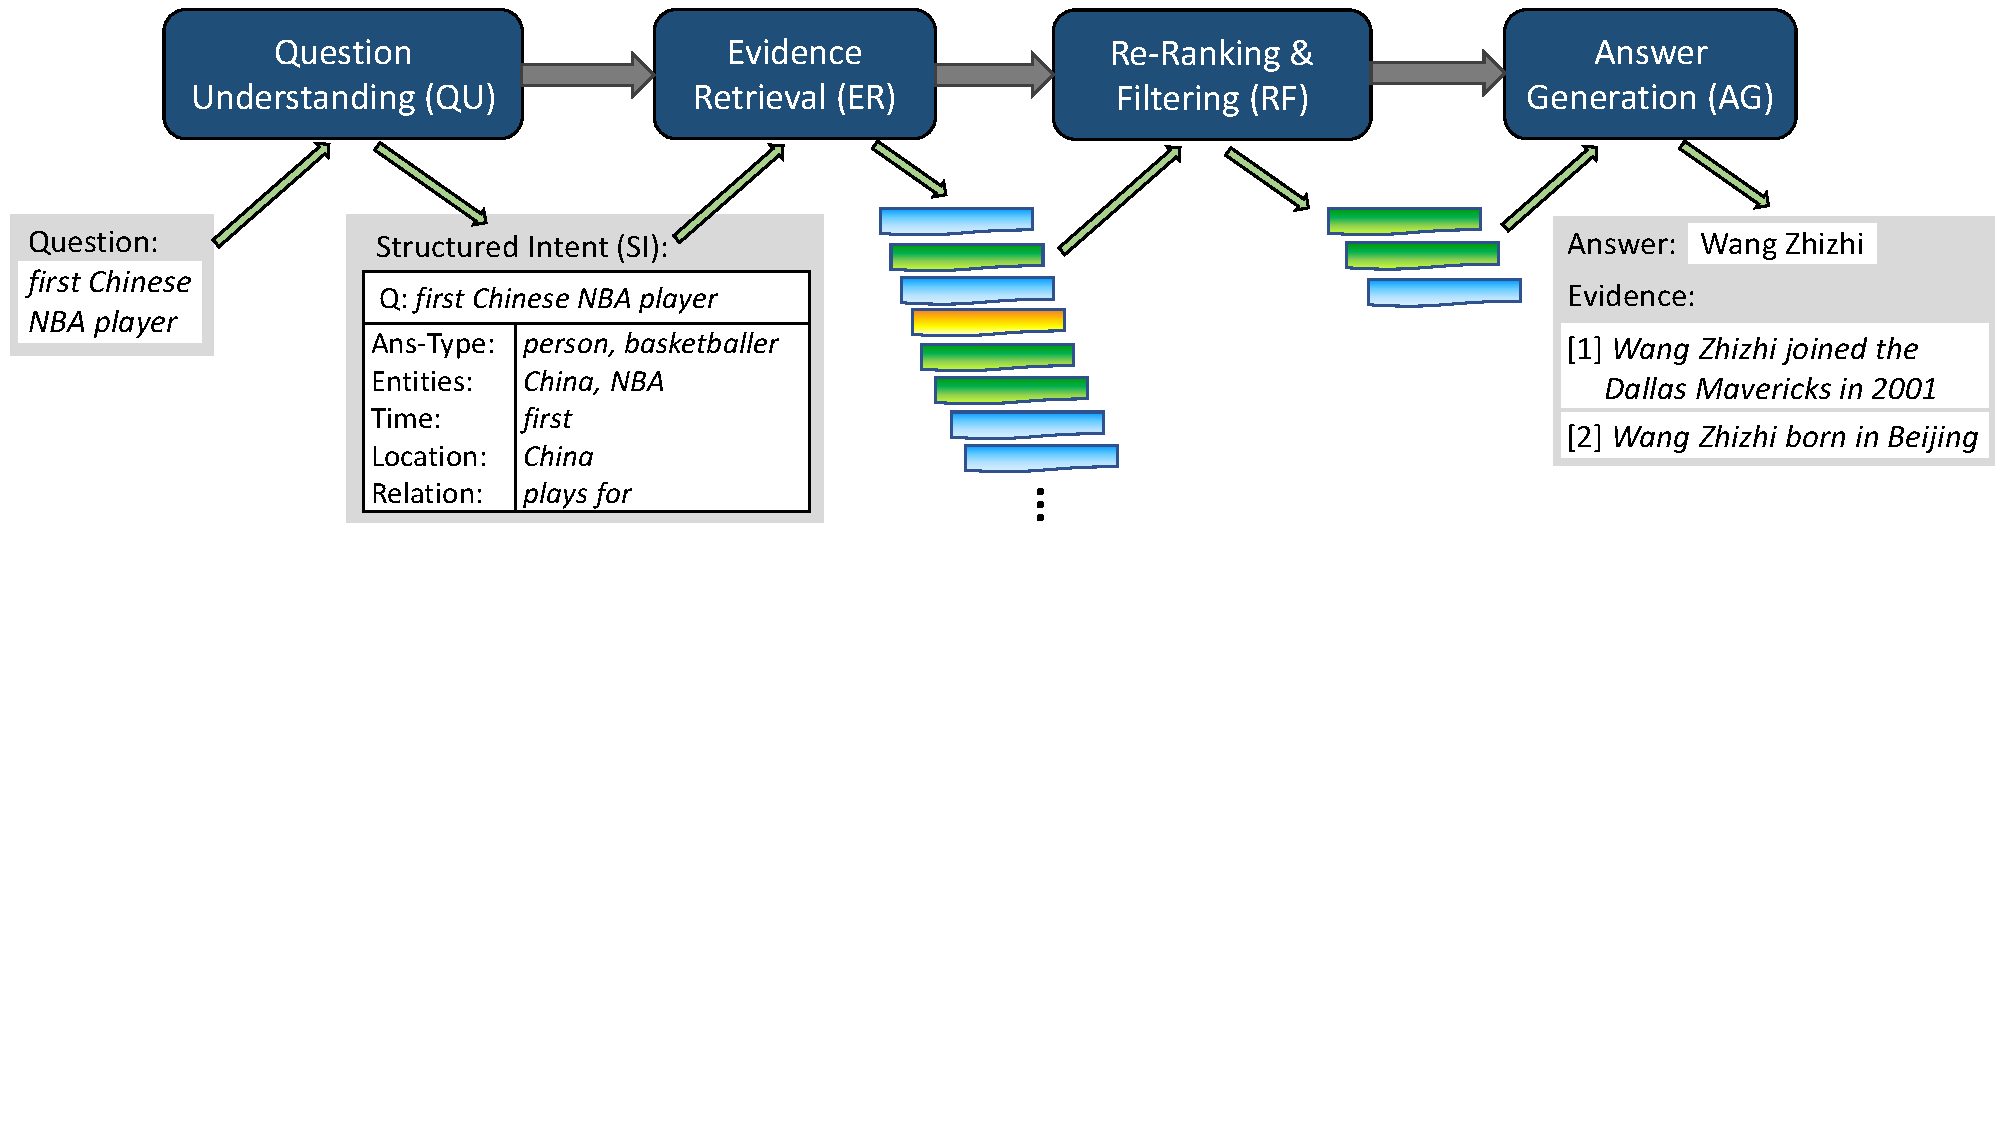
\includegraphics[width=\textwidth]{submissions/Gerhard2024/figures/compass-overview.pdf}
  \caption{Overview of the \method system.}
  \label{fig:compass-overview}
\end{figure}

% start with system overview
The \method system is a pipeline of four major stages, as illustrated in Figure \ref{fig:compass-overview}.
First, the input question is analyzed and decomposed, in order to compute a {\em structured intent (SI)} representation that will pass on to the subsequent steps, along with the original question. Second, the SI is utilized to retrieve pieces of evidence from different sources: text, KG and tables. 
Third, this pool of potentially useful evidence is filtered down, with iterative re-ranking, to arrive at a tractably small set of most promising evidence.
The final stage generates the answer from this evidence,
passing back the answer as well as evidence snippets for user-comprehensible explanation.

The second and fourth stage, Evidence Retrieval (ER) and Answer Generation (AG), are fairly standard. Such a two-phase architecture was called a retriever-reader architecture~\cite{Zhu-ODQA-survey:arxiv2021}. With a modern LLM replacing the earlier kinds of neural readers, this is the core of every RAG system~\cite{DBLP:journals/arXiv/abs-2312-10997}.

Stages 1 and 3 are unique elements of our architecture, judiciously introduced to improve both effectiveness (i.e., answer quality) and efficiency (i.e., computational cost).
Question Understanding (QU) provides the ER component with crisper and semantically refined input, and
the Re-Ranking \& Filtering (RF) stage is beneficial for
distilling the best evidence from the large pool of retrieved pieces.
The following subsections elaborate on the four stages of the pipeline, emphasizing the \method-specific steps QU and RF.



\subsection{Question Understanding (QU)}

% one par introducing the SI
To prepare the retrieval from different kinds of sources, including a KG, ad-hoc tables and text documents, it is useful to analyze and decompose the user question.
In this work, we aim to cast a question into a 
{\em structured intent (SI)} representation: essentially
a frame with faceted cues as slots, or equivalently, a concise set of key-value pairs. 
Figure \ref{fig:compass-overview} gives an idealized example for the question about the first Chinese NBA player. The facets or keys of potential interest here 
are:
\squishlist
\item {\em Ans-Type:} the expected answer type (or types when considering
different levels of semantic refinement), 
\item {\em Entities:} the salient entities in the question, and 
\item {\em Relation:} phrases that indicate which relation (between Q and A entities) the user is interested in. 
\squishend
\noindent In addition, as questions can have temporal or spatial aspects, the SI also foresees slots for:
\squishlist
\item {\em Time:} cues about answer-relevant time points or spans, including relative cues (e.g., ``before Covid'') and ordinal cues (e.g., ``first''), and
\item {\em Location:} cues about answer-relevant geo-locations.
\squishend

% discuss the spectrum of different SIs
\vspace{0.2cm}
\noindent The ideal SI for example question Q2 would look like:

\begin{quote}
{\em Ans-Type:} person, basketballer; {\em Entities:} China, NBA; {\em Time:} first;
{\em Location:} China; {\em Relation:} plays for.
\end{quote}

Note that the values for these slots can be crisp like entity names or dates, but they can also take the form of surface phrases. The SI purpose and value lie in the decomposition. In practice, many questions would only lead to a subset of faceted cues, leaving some slots empty. For the example in Figure \ref{fig:compass-overview}, an alternative SI could simply consist of

\begin{quote}
{\em Ans-Type:} person; {\em Entities:} China, NBA; {\em Time:} first.
\end{quote}

\noindent Even this simplified SI can be highly beneficial in guiding the subsequent evidence retrieval.

% sketch how an LM is trained to generate SIs 
To generate the SI from a user question, we employ a (small-scale) LM, specifically BART~\cite{DBLP:conf/acl/LewisLGGMLSZ20}, a Transformer-based auto-encoder with 140M parameters.\footnote{\url{https://huggingface.co/facebook/bart-base}}
BART is pre-trained for language representation; its power for our purpose comes from fine-tuning.
To this end, we generate (question, SI) pairs by using an instruction-trained LLM like GPT-4, with few-shot in-context learning (following our earlier work~\cite{Jia-FAITH:WWW2024}). 
Note that this is a one-time action; at inference-time we only use much smaller LMs.
The generated silver-standard pairs are then used to fine-tune BART.
In the experiments in this article, we leverage pre-existing collections of silver pairs, based on the training data of the CompMix benchmark~\cite{Christmann-CompMix:WWW2024}, 
comprising $3{,}400$ such pairs.


% outline value of SI for conversations
Although this paper focuses on single-shot questions, the \method architecture is also geared for conversational QA. In that setting, the SI can play an even bigger role, as (follow-up) questions are often formulated in a rather sloppy manner -- all but self-contained. For example, a conversation could start with a clear question {\em When did Wang Zhizhi join the NBA?}, followed a few dialog steps later, by a user utterance like {\em Which teams did he play for?} or simply {\em Which teams?}.
In such an informal conversation, the system needs to {\em contextualize} each user utterance based on the preceding turns in the dialog (e.g., inferring the relevant entities Wang Zhizhi and NBA from the conversational history).
For details on conversational QA, based on our architecture, see our earlier works~\cite{Christmann-CONVINSE:SIGIR2022,Christmann-Explaignn:SIGIR2023}.







%%%%%%%%%%%%%%%%%%%%%%%%%%%%%%%%%%%%%
\subsection{Evidence Retrieval (ER)}

The ER stage taps into a knowledge graph, a corpus of text documents, and a collection of web tables.
Specifically, for the experiments, we use the Wikidata KG,
all English Wikipedia articles, and all tables that are embedded in Wikipedia pages (incl. infoboxes, which can be seen as a special case of tables). 

% specifics: Clocq etc. - and the role of the SI
\vspace{0.2cm}
\noindent{\bf Retrieval from KG:}
To retrieve evidence from the KG, we utilize our earlier work
\clocq~\cite{Christmann-CLOCQ:WSDM2022}, which provides entity disambiguations and a relevant KG-subgraph for a given query.
Unlike most other works on QA-over-KG, \clocq fetches all KG-facts that are relevant for a given entity in a single step.
For example, when querying for
NBA players, it can traverse the KG neighborhood and pick up top teams, also considering so-called qualifier nodes in Wikidata which are often used for temporal scopes. 
As the disambiguation of entity names onto the KG can be tricky and noisy (e.g., China could be mapped to Chinese sports teams in all kinds of sports), \clocq considers several possible disambiguations~\cite{Christmann-CLOCQ:WSDM2022} (typically in the order of $10$ result entities).
The queries for \clocq are 
constructed by concatenating all slots of the question's SI.
For the example query about the first Chinese NBA player,
good result entities would be Dallas Mavericks, lists about NBA seasons, MVP awards etc., and their associated facts. These provide cues, but are likely insufficient to answer the question.


\vspace{0.2cm}
\noindent{\bf Retrieval from Text and Tables:}
The disambiguated entities returned by \clocq form anchors for tapping into text and tables.
\method first identifies 
relevant text documents and tables that refer to the anchor entities. With focus on Wikipedia, these are simply the articles for the respective entities. 
\method then constructs a keyword query that concatenates all available fields of the SI.
The query is evaluated against a linearized and verbalized representation (see below) of all sentences and all table rows in the selected documents.
This returns a set of sentences and 
and individual table rows, ranked by BM25 scores.


\vspace{0.2cm}
\noindent{\bf Evidence Verbalization:}
All results from the different data sources are uniformly treated by {\em linearizing} and {\em verbalizing} them
into token sequences. For KG results, the entity-centric triple sets are linearized via breadth-first traversal of the mini-graph starting from the entity node.
For tables, results are individual rows, which are contextualized by including labels from column headers and from the DOM-tree path of the article where the table comes from. For example, a table row about Wang Zhizhi playing for Dallas (Mavericks) in the 2000-2001 season, would be expressed as:

\vspace{0.05cm}
\hspace*{0.5cm} Wang Zhizhi / NBA Career / Season: 2000-2001, Team: Dallas, Games Played: 5 \dots
\vspace{0.05cm}

\noindent Finally, results from the text corpus are already in the form of token sequences, but we can additionally prefix these with the DOM-tree labels.
We can think of this entire pool of evidence as 
an on-the-fly corpus of potentially relevant pseudo-sentences, forming the input of the subsequent RF stage.


\vspace{0.2cm}
\noindent {\bf Result Ranking:}
Overall, the ER stage compiles a substantial set of evidence, possibly many thousands of entities, text snippets and table rows. Therefore, we practically restrict the pool to a subset of high-scoring pieces, like the top-$1000$.
For scoring, a simple BM25 model (a classical IR method) is applied. 
By default, we treat all evidence pieces uniformly with global scoring, no matter whether they come from KG, text or tables. 


\subsection{Re-Ranking and Filtering (RF)}

With a pool of top-$1000$ evidence pieces, we could invoke an LLM for answer generation. However, that would face a large fraction of noise (i.e., misleading evidence) and incur high costs of computation and energy consumption. 

For both of these reasons, we have devised light-weight techniques for iteratively reducing the top-$1000$ pieces to a small subset, say top-$30$ or top-$10$, that can be fed into an LLM at much lower cost (as LLM computations and pricing are at least linear in the number of input tokens). The difficulty is, of course, to do this without losing good evidence and reducing answer presence. Our techniques for this task are based on graph neural networks (GNNs)~\cite{Wu:IEEE2021} or cross-encoders (CEs)~\cite{Dejean:arxiv2024,Lin:MC2021}.

\myparagraph{GNN-based RF}
Given a large pool of evidence pieces from all sources, a bipartite graph is constructed:
\squishlist
\item {\em nodes} being evidence pieces or entities that occur in these pieces, and
\item {\em edges} connecting an evidence piece and an entity if the entity occurs in the evidence.
\squishend


The task for the GNN is to jointly score the evidence and the entity nodes in a multi-task learning setup. The latter are the {\em answer candidates}, and the evidence should give {\em faithful explanation} for an answer.
We build on our earlier work on explainable QA~\cite{Christmann-Explaignn:SIGIR2023}.

The node encodings are initialized with cross-encoder embeddings (see below) 
for node contents and the SI of the question. The inference iteratively adjusts the encodings based on message passing from neighboring nodes.
The GNN is trained via weak supervision from question-answer pairs:
evidence nodes are labeled as relevant if they are connected to
a gold answer.
More technical details are given in~\cite{Christmann-Explaignn:SIGIR2023}.

\method invokes the GNN in multiple rounds, iteratively reducing top-$k$ to top-$k^*$ nodes with $k^* \ll k$. In practice, we would typically consider two rounds: re-ranking top-$1000$ and pruning to top-100, and then reducing to top-30 or top-10, which are passed to the answer generation stage.
Note that this keeps the GNN at a tightly controlled size, so that its computational costs at inference-time are much smaller than those of an LLM.


\myparagraph{CE-based RF}
An alternative to the GNN inference is to employ a cross-encoder for scoring and re-ranking the evidence pieces.
These are transformers (typically with a small LM like BERT) that are fine-tuned for scoring the relatedness between a query and a document~\cite{Nogueira:arxiv2019}. In our case, the comparison is between the question SI and the evidence piece. In our experiments, we make use of two different cross-encoders, 
both trained on the MS-MARCO benchmark for passage retrieval~\cite{Bajaj:arxiv2018}, 
and fine-tuned on the respective benchmark (leveraging the same weak supervision data as for the GNNs),
the difference being in model size.\footnote{\url{https://huggingface.co/cross-encoder/ms-marco-MiniLM-L-4-v2} and\\ \url{https://huggingface.co/cross-encoder/ms-marco-MiniLM-L-6-v2}}
We use the smaller model to reduce top-$1000$ to top-100, and the larger model to go further down from top-100 to top-30.




%%%%%%%%%%%%%%%%%%%%%%%%%%%%%%%%%%%%%

\subsection{Answer Generation (AG)}

The last stage follows mainstream practice to invoke an LLM in a retrieval-augmented manner.
We call a `small-scale` LLM, specifically a fine-tuned LlaMA-3.1 model (8B-Instruct)\footnote{\url{https://huggingface.co/meta-llama/Llama-3.1-8B-Instruct}}, with a prompt \footnote{The specific prompt is \phrase{SI: \textless\texttt{concatenated SI}\textgreater \hspace{0.1cm} Evidence: \textless\texttt{evidence pieces}\textgreater}.}
consisting of:

\squishlist
\item the concatenated SI of the original question, and
\item the top-30 (or other top-$k^*$ with small $k^*$) evidence pieces.
\squishend

By the previous down-filtering of the original pool of evidence pieces, this last step has affordable cost in terms of computation time and energy consumption.

\vspace{0.2cm}
\noindent{\bf Fine-Tuning the LLM:}
We considered adding an instruction to the prompting, such as {\em ``answer this question solely based on the provided evidence snippets''}.
However, this turned out to be ineffective.
The reason why the model works well without such instructions is our task-specific fine-tuning.
We perform this by running the training data of benchmarks through the \method pipeline,
and training the AG stage with the top-30 evidence pieces as input.
Thus, the fine-tuning makes the model learn the role of evidence for RAG-based QA.

\vspace{0.2cm}
\noindent{\bf Explanations:}
The top-30 evidence pieces can be used to provide users with explanation of answers.
Optionally, these could be reduced further for comprehensibility.
Alternatively, we can fine-tune the LLM to provide both answers and concise explanations.
Since we can infer which evidences in the input mention the annotated ground-truth answers,
our method could be fine-tuned to provide such \textit{answering evidences} as well (cf.~\cite{Gao-citations:emnlp2023}).

\label{sec:exp}
\section{Experiments}


\label{setup}
\subsection{Experimental setup}


%%% BENCHMARKS
\myparagraphnospace{Benchmarks} We run experiments on three benchmarks with different characteristics of questions.

\squishlist
    \item \textbf{\compmix}.
    \compmix~\cite{Christmann-CompMix:WWW2024} is a benchmark which was specifically designed for evaluating QA systems operating over heterogeneous sources. The dataset has $9{,}410$ questions, out of which $2{,}764$ are used for testing.
    Answers are crisp entity names, dates, or other literals.
    
    \item \textbf{\crag}.
    We further evaluate on a subset of the \crag~\cite{Yang-CRAG} dataset, which was recently released as a testbed for RAG-based QA systems.
    We utilize the same pipeline and sources as outlined in Section~\ref{sec:method}, without using the web snippets or APIs provided with \crag. This way we focus on entity-centric questions that do not require access to live web data (e.g., news feeds), and disregard cases where the results would be up-to-date quantities.
    This restricts the test data to $436$ entity-centric questions, still enough for a proof of concept.
    
    \item \textbf{\timequestions}.
    To showcase the generalizability of our pipeline, we conduct experiments on~\timequestions~\cite{Jia-TimeQuestions},
    a benchmark for temporal QA. The dataset requires temporal understanding and reasoning, which are well-known limitations of
    LLMs~\cite{Dhingra-time-aware-LLM:TACL2022}. \timequestions has 16{,}181 questions (3{,}237 for testing).
\squishend

Typical examples for the questions in these three benchmarks are:

\begin{quote}
\compmix: \utterance{Which player won the most number of Man-of-the-Match titles in the FIFA world cup of 2006?}\\
 \indent \crag: \utterance{What was the worldwide box office sales for little hercules?}\\ 
  \indent \timequestions: \utterance{Which club did Cristiano Ronaldo play for before joining Real Madrid?}
\end{quote}

%%% BASELINES
\myparagraph{Baselines} As competitors or reference points to \method, we study the performance of the following methods:

\squishlist
    \item \textbf{Generative LLMs}.
    We compare \method against out-of-the-box LLMs: \textbf{\gptthree} (\texttt{text-davinci-003}), \textbf{\gptfour} (\texttt{gpt-4}) 
    and \textbf{\llama} (\texttt{meta-llama/Llama-3.1-8B-Instruct}).
    The same prompt is used for all LLMs, consistent with previous work~\cite{Christmann-CompMix:WWW2024, Zhang-Spaghetti:ACL2024}:
    \phrase{Please answer the following question by providing the crisp answer entity, date, year, or numeric number. Q: \textless\texttt{question}\textgreater}.
    

    \item \textbf{Heterogeneous QA methods}.
    \convinse~\cite{Christmann-CONVINSE:SIGIR2022}, \unikqa~\cite{Oguz-UniK-QA:NAACL2022}, \explaignn~\cite{Christmann-Explaignn:SIGIR2023}
    are QA methods designed to integrate heterogeneous sources: text, tables and KG. All of these  integrate the exact same sources as \method.

    
    \item \textbf{\textsc{State-of-the-art}}.
    For \compmix and \timequestions, we also compare against state-of-the-art methods from the literature: \spaghetti~\cite{Zhang-Spaghetti:ACL2024} and \textsc{Un-Faith}~\cite{Jia-FAITH:WWW2024}, which are among the best performing systems.
    
Results are taken from the literature whenever applicable.
On \crag, we use the models trained on \compmix for \method and heterogeneous QA baselines.
\squishend



%%% METRIC(S)
\myparagraph{Metrics}
We measure \textit{precision at 1} (\textbf{P@1}) as our main metric~\cite{RoyAnand:MC2021} on all benchmarks.
On \crag, we manually annotate answer correctness, as the ground-truth answer formats vary (e.g., entity name variants, lists, sentences).

We also compute the number of neural parameters aggregated over all sub-modules (\textbf{\#Parameters}).
Parameter counts for GPT-models are taken from~\cite{Minaee-LLM-survey}
(\gptfour might have less active parameters during inference).

For further analysis we measure \textit{answer presence} (\textbf{AP@k}),
i.e. whether the answer is present in the top-$k$ ranked evidence pieces,
and \textit{mean reciprocal rank} within the top-$k$ evidences (\textbf{MRR@k}).

%%% CONFIG
\myparagraph{Configuration}
Our implementation uses the \texttt{Llama3.1-8B-Instruct} model for the AG stage.
For the QU, ER and RF stages
we adopt code from the \explaignn project.\footnote{\url{https://explaignn.mpi-inf.mpg.de}}
For the ER stage, we use \clocq, setting its specific parameters to $k=10$ and $p=1{,}000$.

As default, we use the GNN technique for the RF stage.
For efficiency, we use light-weight models for initializing
the GNN encoders -- the same models used for the CE-based RF.\footnote{\url{https://huggingface.co/cross-encoder/ms-marco-MiniLM-L-4-v2} and\\\url{https://huggingface.co/cross-encoder/ms-marco-MiniLM-L-6-v2}}
The GNNs are trained for $5$ epochs with an epoch-wise evaluation strategy,
i.e. we choose the model with the best performance on the respective dev set.
We train the GNNs on graphs with a maximum of $100$ evidence and $400$ entity nodes (as scored by BM25).
During inference, the first GNN is applied on graphs with $1{,}000$ evidence and $4{,}000$ entity nodes, shrinking the pool of evidence pieces to the top-$100$.
The second GNN then runs on graphs with $100$ evidence and $400$ entity nodes.
The factor of 4 entities per evidence (on average) holds sufficient for the observed data,
and enables batched inference.
Other parameters are kept as is.

The AG model, based on \texttt{Llama3.1-8B-Instruct}, is 
fine-tuned
for $2$ epochs with a warm-up ratio of $0.01$ and a batch size of $8$, again with an epoch-wise evaluation strategy.
Other parameters are set to the default Hugging Face
training parameters.\footnote{\url{https://huggingface.co/docs/transformers/v4.46.2/en/main_classes/trainer\#transformers.TrainingArguments}}





\subsection{Main results}
%%% MAIN TABLE
\myparagraphnospace{\method is competitive on all benchmarks}
Main results of our experiments are shown in Table~\ref{tab:main-res}.
First of all, we note that \method achieves competitive performance across all three benchmarks.

On \compmix, baselines for heterogeneous QA and \llama perform similarly,
whereas GPT-based LLMs can answer more than $50$\% of the questions correctly.
\method exhibits substantially higher performance, on par with
the state-of-the-art method \textsc{Spaghetti}~\cite{Zhang-Spaghetti:ACL2024}
(which is based on \gptfour).

On the \crag dataset, P@1 drops for all methods except for \gptfour. 
The benchmark includes realistic questions,
which can be ambiguous/confusing (\phrase{who was the director for the report?}),
on ``exotic'' entities with answers in social media (\phrase{how many members does the teknoist have?}),
or require up-to-date information (\phrase{when did chris brown release a song or album the last time?}),
and other cases that are challenging for all methods.

Finally, \method establishes new state-of-the-art performance on the \timequestions benchmark.
Interestingly, all of the tested LLMs show greatly reduced performance on this benchmark,
which inherently requires temporal understanding and reasoning
-- a known weakness of stand-alone LLMs.


\begin{table} [h]
    \centering
    \newcolumntype{G}{>{\columncolor [gray] {0.90}}c}
    \begin{tabular}{l G G G c}
        \toprule
            \textbf{Method $\downarrow$ / Benchmark $\rightarrow$} & \textbf{\compmix}  & \textbf{\crag} & \textbf{\timequestions} & \textbf{\#Parameters} \\ 
        \midrule
            \textbf{\gptthree} 
            & $0.502$ &   $-$ & $0.224$ & $175{,}000$ M  \\
            % #params from https://arxiv.org/pdf/2402.06196

            \textbf{\gptfour}
            & $0.528$ &   $\mathbf{0.633}$ & $0.306$ & $1{,}760{,}000$ M \\
            % #params from https://arxiv.org/pdf/2402.06196

            \textbf{\llama~\cite{Touvron-LLaMA}} (8B-Instruct)
            & $0.431$ &   $0.385$ & $0.178$ & $8{,}030$ M  \\
            % #params from Huggingface (8,030,257,152)
        \midrule
            \textbf{\convinse~\cite{Christmann-CONVINSE:SIGIR2022}}
            & $0.407$  &   $0.298$ & $0.423$  & $362$ M \\
            % FiD: 222,903,936 + BART (SR-generation): 139,420,416 = 362,324,352 (python explaignn/question_understanding/structured_representation/get_num_params.py)

            \textbf{\unikqa~\cite{Oguz-UniK-QA:NAACL2022}}
            & $0.440$ &   $0.280$ & $0.424$ & $223$ M  \\
            % FiD: 222,903,936 (python explaignn/heterogeneous_answering/fid_module/FiD/get_num_params.py)
    
            \textbf{\explaignn~\cite{Christmann-Explaignn:SIGIR2023}} 
            & $0.442$ &   $0.303$ & $0.525$  & $328$ M \\
            % BART (SR-generation): 139,420,416 + 2GNNs: 94520832 + 93930240 = 327,871,488

        \midrule 
            \textbf{\textsc{State-of-the-art}}
            & $\mathbf{0.565}$ 
            & $-$
            & $0.571$  & $-$ \\

            & (\textsc{Spaghetti}~\cite{Zhang-Spaghetti:ACL2024})
            & 
            & (\textsc{Un-Faith}~\cite{Jia-FAITH:WWW2024}) &  \\

        \midrule
            \textbf{\method (ours)}
            & ${0.564}$ &   $0.362$ & $\mathbf{0.754}$  & $8{,}218$ M \\
            % BART (SR-generation): 139,420,416 + LLaMA: 8,030,257,152 + GNNs: 25,670,016 + 22,268,928 =  8,217,616,510
        \bottomrule
    \end{tabular} 
    \vspace*{-0.2cm}
    \caption{End-to-end P@1 of \method and baselines on three benchmarks. Results for \gptthree and \gptfour are taken from the literature~\cite{Christmann-CompMix:WWW2024, Jia-FAITH:WWW2024}. \gptthree is not accessible anymore, hence no results on \crag.
    }
    \label{tab:main-res}
\end{table}





%%% ANSWER SOURCES
\myparagraph{Integration of heterogeneous sources is vital}
\method integrates evidence from text, KG and tables into a unified framework.
We aim to better understand how this affects the answering performance of the method.
Table~\ref{tab:sources} shows end-to-end answering performance of \method
with different combinations of the input sources.
The results clearly indicate that all types of sources contribute, with option Text+KG+Tables performing best,
with a large margin over tapping only single source types.

\begin{table} [t] 
    \centering
    \newcolumntype{G}{>{\columncolor [gray] {0.90}}c}
    \newcolumntype{H}{>{\setbox0=\hbox\bgroup}c<{\egroup}@{}}
    	\begin{tabular}{l G G G H H H c c c} 
        \toprule
            \textbf{Benchmark $\rightarrow$}
                & \multicolumn{3}{G}{\textbf{\compmix}} 
                & \multicolumn{3}{H}{\textbf{\crag}}
                & \multicolumn{3}{c}{\textbf{\timequestions}} \\ 
        \midrule
            \textbf{Input sources $\downarrow$ / Metric $\rightarrow$}
                & \textbf{P@1} & \textbf{AP@100}  & \textbf{AP@30}
                & \textbf{P@1} & \textbf{AP@100}  & \textbf{AP@30}
                & \textbf{P@1} & \textbf{AP@100}  & \textbf{AP@30} \\
            \midrule
                \textbf{Text}           &  $0.455$  &  $0.563$  &  $0.531$ &  $?$  &  $?$  &  $?$ &  $0.539$  &  $0.515$  &  $0.487$   \\
                \textbf{KG}             &  $0.481$  &  $0.677$  &  $0.637$ &  $?$  &  $?$  &  $?$ &  $0.724$  &  $0.701$  &  $0.674$   \\
                \textbf{Tables}         &  $0.432$  &  $0.501$  &  $0.482$ &  $?$  &  $?$  &  $?$ &  $0.536$  &  $0.347$  &  $0.328$   \\
            \midrule
                \textbf{Text+KG}        &  $0.537$  &  $0.749$  &  $0.706$ &  $?$  &  $?$  &  $?$ &  $0.745$  &  $\mathbf{0.776}$  &  $0.748$   \\
                \textbf{Text+Tables}    &  $0.503$  &  $0.632$  &  $0.594$ &  $?$  &  $?$  &  $?$ &  $0.567$  &  $0.578$  &  $0.549$   \\
                \textbf{KG+Tables}      &  $0.524$  &  $0.728$  &  $0.692$ &  $?$  &  $?$  &  $?$ &  $ 0.743$  &  $0.731$  &  $0.703$   \\
            \midrule
                \textbf{Text+KG+Tables}    &  $\mathbf{0.564}$  &  $\mathbf{0.759}$  &  $\mathbf{0.724}$ &  $?$ &  $?$  &  $?$ & $\mathbf{0.754}$    & $\mathbf{0.776}$  &  $\mathbf{0.749}$   \\
            \bottomrule
    \end{tabular}
    \vspace*{-0.2cm}
    \caption{Answer presence and answering precision of \method with different combinations of input sources (on the respective test sets).}
    \label{tab:sources}
\end{table}




\subsection{Analysis}

%%% TOP-K vs. 3xTOP-(K/3)
\myparagraph{Unified retrieval enhances performance}
In the RF stage, we re-rank and filter evidence from different source types,
and feed the unified top-\textit{k}* into the AG stage.
We conduct a comparison in which we consider
the top-$10$ evidence pieces from each source type individually. This gives equal influence to KG, text and tables, whereas our default is based on global ranking.
Table~\ref{tab:unified-retrieval} shows the results for this analysis, showing our default choice performs better.
The reason is that different questions require different amounts of evidence from each of the source types.

\begin{table} [t] 
    \centering
    \newcolumntype{G}{>{\columncolor [gray] {0.90}}c}
    \newcolumntype{H}{>{\setbox0=\hbox\bgroup}c<{\egroup}@{}}
    	\begin{tabular}{l G G H H} 
        \toprule
            \textbf{Input evidences $\downarrow$ / Metric $\rightarrow$} & \textbf{P@1} & \textbf{AP@30}  & \textbf{\crag} & \textbf{\timequestions} \\ 
            \midrule
                \textbf{Top-30 Text+KG+Tables (ours)}             &  $\mathbf{0.574}$  &  $\mathbf{0.710}$  &  $-$  &  $-$   \\
                \textbf{Top-10 Text + Top-10 KG + Top-10 Tables}        &  $0.560$    &  $0.709$  &  $-$  &  $-$   \\
            \bottomrule
    \end{tabular}
    \vspace*{-0.2cm}
    \caption{Answer presence and precision
    of \method for different choices of top-30 
    (on \compmix dev set).}
    \label{tab:unified-retrieval}
\end{table}


%%% NUMBER OF EVIDENCES
\myparagraph{\method works well with small amounts of evidence}
We investigate the 
influence of 
the number of evidence pieces
fed into the AG stage, varying it from $5$ to $100$.
Results are shown in Figure~\ref{fig:res-num-evidences}.
As the curve shows, there is a sharp increase in precision as we add evidence up to 30 or 40 pieces, which is around our default of top-30. This indicates that a certain amount of evidence is needed, to overcome the inherent noise and arrive at sufficient answer presence. 
As we increase the amount of evidence further, we observe a saturation effect, and eventually a degration of performance. Too much evidence not only has diminishing returns, but can actually be confusing for the AG stage. This reconfirms our heuristic choice of top-30: enough for good answering while keeping computational costs reasonably low.


\begin{figure}[t]
    \centering
    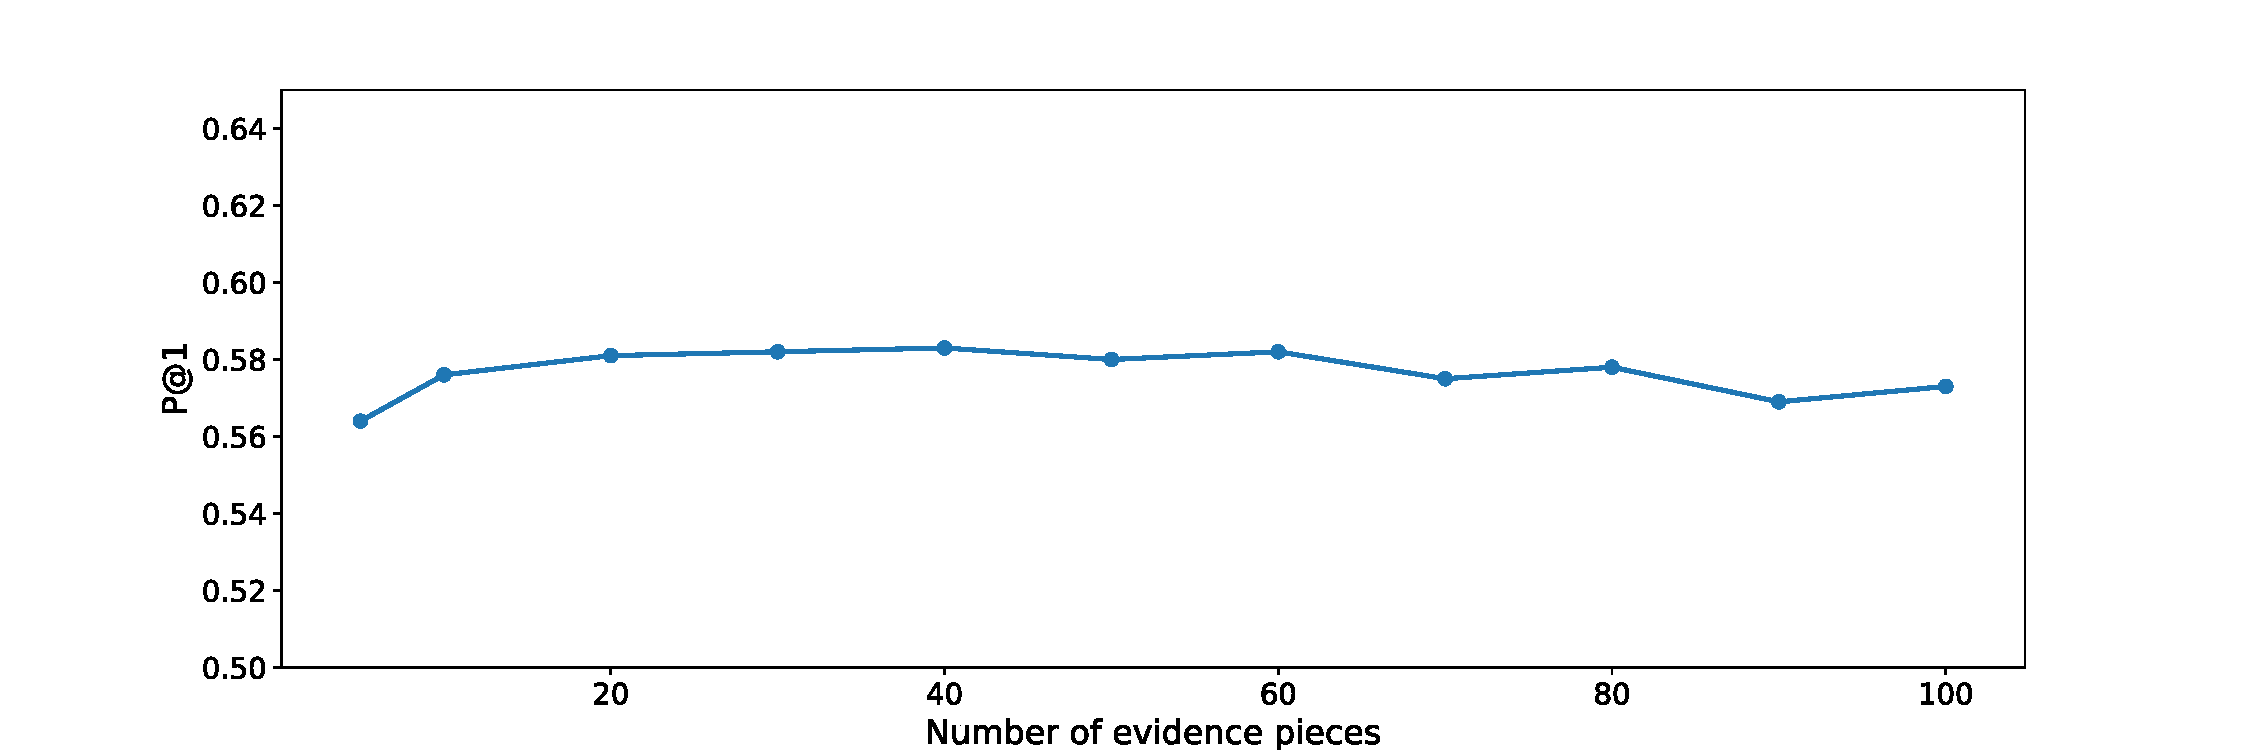
\includegraphics[width=0.8\textwidth]{submissions/Gerhard2024/figures/p_at_1-line_with_evidences.pdf}
    \vspace*{-0.2cm}
    \caption{Performance of \method on the \compmix dev set with different numbers of evidence.}
    \label{fig:res-num-evidences}
    \vspace*{-0.2cm}
\end{figure}



%%% ABLATION
\myparagraph{Ablation study on re-ranking} For more insight on the possible configurations of the RF stage, we conducted an ablation study with different options, including solely relying on the initial BM25 scoring without explicit re-ranking. The results are shown in Table \ref{tab:ablation2}. We observe that the iterative reduction in two steps is slightly better than the single-step variants (going down from top-1000 to top-30 in one RF step). Between the two options of using a GNN or a CE, the differences are negligible. A notable effect is that our RF techniques retain the answer presence at a very high level, only a bit lower than for the initial top-1000. 
The last two rows of Table \ref{tab:ablation2} demonstrate that RF is crucial: without explicit re-ranking, the technique of just picking smaller top-$k$ from the original BM25 model leads to substantial degradation in both answer presence and precision. 


\begin{table} [t] \small
    \centering
    \newcolumntype{G}{>{\columncolor [gray] {0.90}}c}
    \newcolumntype{H}{>{\setbox0=\hbox\bgroup}c<{\egroup}@{}}
    	\begin{tabular}{l G H G G G} 
        \toprule
            & \multicolumn{5}{G}{\textbf{\compmix} (dev set)} \\
        \midrule
            \textbf{RF Method $\downarrow$ / Metric $\rightarrow$} & \textbf{P@1} & \textbf{AP@1000} & \textbf{AP@100}  & \textbf{AP@30} & \textbf{MRR@100} \\ 
        \midrule
            \textbf{GNN: 1000 $\rightarrow$ 100 $\rightarrow$ 30}             &  $\mathbf{0.574}$  & $0.760$ &  $0.738$  &  $0.710$  &  $\mathbf{0.572}$  \\
            \textbf{CE: 1000 $\rightarrow$ 100 $\rightarrow$ 30}          &  $0.573$  & $0.760$  &   $\mathbf{0.740}$ &  $\mathbf{0.721}$   &  $0.553$   \\
        \midrule
            \textbf{GNN: 1000 $\rightarrow$ 30} &  $0.567$  & $?$  &   $n/a$ &  $0.710$   &  $0.567$   \\
         \textbf{CE: 1000 $\rightarrow$ 30} &  $0.570$  & $0.760$  &   $n/a$ &  $0.715$   &  $0.558$   \\
            \midrule
           \textbf{BM25: 100 (w/o GNN or CE)} &  $0.490$ & $0.760$  &  $0.652$  &  $n/a$  &  $0.259$ \\       
            \textbf{BM25: 30 (w/o GNN or CE)} &  $0.468$  & $0.760$  &  $n/a$ &  $0.534$   &  $0.259$   \\
            \bottomrule
    \end{tabular}
    \vspace*{-0.2cm}
    \caption{Ablation study for different RF strategies of \method on the \compmix dev set. The answer presence in the RF input with top-$1000$ evidence pieces is $0.760$.}
    \label{tab:ablation2}
\end{table}



\myparagraph{Quality of SI}
To assess the quality and robustness of the Structured Intents, we
inspected a sample of questions and their SIs.
Table~\ref{tab:question-SI-examples} gives three anecdotic examples.
We show SIs generated by \method, which makes use of the pre-existing collection from the \compmix benchmark for training.
This training data was obtained via different heuristics, 
which can be a limiting factor when user intents become more complex.

Therefore, we also looked at SIs derived via in-context learning (ICL) using \gptfour with $5$ handcrafted examples.
As shown in our earlier work on temporal QA~\cite{Jia-FAITH:WWW2024},
such data can be used for training smaller models (e.g., BART),
which can greatly boost the completeness and overall quality of the generated SIs.

From the sampled set, we observed that the ICL-based SIs are more
complete with all slots filled, whereas the BART-based SIs focused more
on the main slots Answer-type, Entities and Relation.
However, both approaches achieve very high quality in filling the slots,
capturing the user's information need very well.

Interestingly, when questions get complicated, with nested phrases, 
the ICL-based variant succeeds in decomposing the questions, based on only $5$ ICL examples.
For example, for the question {\em ``which German state had the most Corona-related death cases in the first year after the outbreak?''}
the Time slot becomes {\em ``first year after Corona outbreak''},
which can be resolved to identify the temporal scope.
In general, we believe that such question decomposition, beyond simple temporal constraints,
would be an interesting theme for future work.

\begin{table} [t] 
    \centering
    \small
    \newcolumntype{G}{>{\columncolor [gray] {0.90}}c}
    \newcolumntype{H}{>{\setbox0=\hbox\bgroup}c<{\egroup}@{}}
    \resizebox*{\textwidth}{!}{
        \begin{tabular}{p{6cm}|p{6cm}|p{6cm}} 
        \toprule
            \textbf{Question} & \textbf{Current SI by \method} & \textbf{SI via ICL} \\
        \midrule
        \textit{what was disneys first color movie?}
            & Ans-Type: \textit{animated feature film} & Ans-Type: \textit{film, animated film} \\
            & Entities: \textit{disneys} & Entities: \textit{Disney} \\
            & Relation: \textit{was first color movie} & Relation: \textit{first color movie} \\
            &  & Time: \textit{first} \\
        \midrule
        \textit{at the oscars, who won best actor in 2018?}
            & Ans-Type: \textit{human} & Ans-Type: \textit{person, actor} \\
            & Entities: \textit{at the oscars} & Entities: \textit{Oscars, 2018} \\
            & Relation: \textit{who won best actor in 2018} & Relation: \textit{won best actor} \\
            &  & Time: \textit{2018} \\
        \midrule
        \textit{which German state had the most Corona-} & Ans-Type: \textit{state} & Ans-Type: \textit{location, state} \\
        \textit{related death cases in the first year after} & Entities: \textit{Germany, Corona} & Entities: \textit{Germany, Corona-related deaths} \\
        \textit{the outbreak?} & Relation: \textit{which state had the most related} & Relation: \textit{highest count of death cases} \\
        & \textit{death cases in the first year after the out-}  & Location: \textit{Germany} \\
            & \textit{break}  & Time: \textit{first year after Corona outbreak} \\
        \bottomrule
    \end{tabular}
    }
    \vspace*{-0.2cm}
    \caption{Examples for pairs of question and generated SI.}
    \label{tab:question-SI-examples}
\end{table}




%%% REFRAIN FROM ANSWER
\myparagraph{Refraining from answering}
%%% Searched for: "generated_answer I" (with I being the full word, not partial) in the generated answers of LLaMA
%%% yields 245 results out of 2764 questions on CompMix
%%% yields 1270 results out of 3237 questions on TimeQuestions
We can train our model to refrain from answering in scenarios
where the provided evidence does not contain an answer to the question.
Specifically, during training, when the answer is not present in the evidence,
we change the target answer to {\em unknown}. This variant is referred to as \method {\em (faithful)}.

We measure the ratio of questions for which {\em unknown} is provided as answer,
and the P@1 restricted to questions that are answered.
The accuracy of refraining from answering is measured as well,
based on whether the answer is present in the evidence or not.
We conduct this experiment on \compmix and \timequestions,
for which we can compute answer presence exactly.
We also compute results for \llama, which is already instructed 
with the option to answer ``don't know''.
Table~\ref{tab:refrain-from-answer} shows the results.
For \compmix, we observe that \method has high accuracy on refraining when appropriate,
whereas \llama tends to be overconfident with a very small rate of {\em unknowns}, leading to incorrect answers.

\begin{table} [t] \small
    \centering
    \newcolumntype{G}{>{\columncolor [gray] {0.90}}c}
    \newcolumntype{H}{>{\setbox0=\hbox\bgroup}c<{\egroup}@{}}
    	\begin{tabular}{l G G G G c c c c} 
        \toprule
            & \multicolumn{4}{G}{\textbf{\compmix}} & \multicolumn{4}{c}{\textbf{\timequestions}} \\
            \midrule
            \textbf{Metric $\rightarrow$} & \textbf{P@1}  & \textbf{P@1} & \textbf{Refrain} & \textbf{Refrain} & \textbf{P@1}  & \textbf{P@1} & \textbf{Refrain} & \textbf{Refrain} \\ 
            \textbf{Method $\downarrow$} &                 & \textbf{(answered)} & \textbf{rate} & \textbf{accuracy} &                 & \textbf{(answered)} & \textbf{rate} & \textbf{accuracy} \\ 
            \midrule
                \textbf{\llama}             &  $0.431$  &  $0.471$  &  $0.089$  &  $n/a$  &  $0.177$  &  $0.276$  &  $0.392$  &  $n/a$  \\
                \textbf{\method (faithful)}           &  $0.497$  &  $0.713$  &  $0.303$  &  $0.838$ &  $0.597$  &  $0.804$  &  $0.257$  &  $0.864$  \\
            \bottomrule
    \end{tabular}
    \vspace*{-0.2cm}
    \caption{
        Performance of \method with option to refrain from answering (``don't know'').
    }
    \label{tab:refrain-from-answer}
\end{table}

\label{sec:disc}
\section{Insights, Limitations, and Challenges}


\noindent{\bf Benchmark Performance.} Our method, RAG-based \method with an 8B LLaMA model, outperforms much larger LLMs like \gptfour on two of the three benchmarks, with a very large margin for temporal questions. Obviously, pre-trained LLMs have only limited sense of properly positioning ``remembered’’ facts on the timeline even with training data that exceeds ours by several orders of magnitude. This confirms our intuition that LLMs alone are not good at ``recalling’’  higher-arity relations that require combining distant pieces of evidence. This is a sweet spot for RAG. Only for 
the \crag benchmark, \method is substantially inferior to a full-blown LLM. This is likely due to the nature of the questions: not necessarily the complexity of the information needs, but the need for more web sources (beyond what our experiments tap into).

\vspace{0.2cm}
\noindent{\bf Cost/Performance Ratio.} The most important take-away from our experiments is that \method achieves its competitive performance at a much lower cost than the full LLMs. Assuming that the consumed GFlops are proportional to the number of model parameters, \method achieves a cost reduction by a factor of 200x for \gptthree and 2000x for \gptfour. This does not only mean less computation, but also a massively lower electricity bill and climate impact.  

\vspace{0.2cm}
\noindent{\bf Role of Question Understanding.} We did not systematically investigate the influence of the Structured Intent in the \method pipeline. However, the comparison to the big GPT models reflects the role of the SI, as we prompt the GPT models in their natural mode with the original questions. The linearized sequence of available SI slots does not always have major advantages, but there are enough cases where specific facets provide crucial cues. This holds especially for the Entities slot, as this drives the gathering of evidence in the ER stage (cf.~\cite{Christmann-CONVINSE:SIGIR2022}, and for the Time slot, as these cues are often decisive for temporal questions (cf.~\cite{Jia-FAITH:WWW2024}).

\vspace{0.2cm}
\noindent{\bf Role of Re-Ranking.} As our ablation studies show, merely using top-$k$ evidence from an initial BM25-style ranking does not provide good performance. Also, there seems to be sweet spot in the choice of $k$: we need enough evidence for connecting the dots if the question requires multiple pieces of information, or for corroborating candidates if the question finds many useful but noisy pieces. In the experiments, $k=30$ turns out to be good choice; much lower $k$ results in insufficient evidence, and much larger $k$ leads to saturation and ultimately degrading performance. Our argument for iteratively shrinking the candidate set in multiple rounds of re-ranking is substantiated in our experiments, but the gain of doing this, compared to GNN- or CE-based re-ranking from 1000 to 30, is not big. More research is called to better understand the role of ranking in RAG. 

\vspace{0.2cm}
\noindent{\bf Limitations of Evidence Retrieval.}
For ER, we adopted more or less standard techniques. The results showed very good answer presence, in the order of 75\% in the top-100 or even top-30. An important case where this is insufficient are questions that require aggregating information over a large number of evidence pieces. An example is asking for the life-time total of 3-point scores of the basketball player Dirk Nowitzki.
This requires collecting a set of per-season tables with NBA player statistics, but also other web sources with numbers for his career before he joined the NBA (including his youth teams).
Of course, there are sometimes shortcuts like a Wikipedia article or biography mentioning the total number, but this cannot be universally assumed. The bottom line is that ER should be reconsidered as well, striving to improve the recall dimension.

\vspace{0.2cm}
\noindent{\bf Limitations of Answer Generation.}
For AG, we simply rely on a LLM,
using it as an extractor (``reader'') from the given evidence. Despite the wide belief that LLMs can perform deep
reasoning over many pieces of evidence, our experience is that the extraction works only well – robustly and faithfully – for relatively simple questions with a few multi-hop joins or simple aggregation over a few pieces. However, complicated questions such as asking for the top-100 NBA players with the largest number of life-time 3-point scores (again including their pre-NBA careers) are currently out of scope and will likely remain so for quite some time. This offers many opportunities for pushing the envelope further.

\vspace{0.2cm}
\noindent{\bf Trust in Data Sources.}
In our experiments, we considered all heterogeneous sources as trustworthy and unbiased. With focus on Wikidata and Wikipedia, this assumption has been well justified. In the wild, however, input data for RAG-based systems likely exhibit a wide spectrum of quality issues, in terms of stale information, biased positions, or simply false statements. Identifying trustworthy and up-to-date evidence and dealing with conflicting data, has been explored in other contexts (e.g., for KG curation~\cite{Dong-Trust:PVLDB2015}), but remains a major challenge for RAG-based QA.


\vspace{0.2cm}
\noindent{\bf Open Challenges and Future Work.} The best-performing methods in our experiment, mostly \method, reach P@1 values of 56\% for \compmix and 75\% for \timequestions. 
For the latter, the answer presence in the top-100 is only slightly higher; so the AG stage hardly misses anything.
However, for \compmix, the answer presence is 75\% -- much higher than what our system can actually answer. Obviously, closing this gap is a major direction to pursue, with focus on the RF and AG stages. However, missing one fourth of the answers completely in the top-100 pool, is a big problem as well. This requires improving recall at the ER stage, possibly with better guidance by the QU, which in turn needs more sources beyond the scope of our experiments (currently limited to Wikidata and Wikipedia). 

In general, we need to think beyond this kind of ``benchmark mindset’’. Even if we reached 80\% or 90\% precision and recall, we would still have a substantial fraction of questions that are answered incorrectly
or not at all. 
The remaining errors may not be a problem for chatbots, but they would be a showstopper for the deployment of mission-critical applications in business or science. We believe that this big gap is a shortcoming of {\em all methods}, not an issue that comes from the data alone. For trivia-style QA, as looked at in this paper, a smart human in ``open book’’ mode and no time limitation should be able to properly answer practically all questions, just by reading pieces of web contents and putting things together. Neither LLMs nor state-of-the-art RAG are the final solution; substantial research and creative ideas are needed to further advance QA.


\clearpage
\newpage

\newcommand{\bibauthors}[1]{{#1}}
\newcommand{\bibtitle}[1]{\emph{#1}}
\newcommand{\bibconf}[1]{{#1}}

\begin{thebibliography}{10}

\bibitem{Bajaj:arxiv2018}
\bibauthors{Payal Bajaj, Daniel Campos, Nick Craswell, Li Deng, Jianfeng Gao, Xiaodong Liu, Rangan Majumder, Andrew McNamara, Bhaskar Mitra, Tri Nguyen, Mir Rosenberg, Xia Song, Alina Stoica, Saurabh Tiwary, Tong Wang.}
\bibtitle{MS MARCO: A Human Generated MAchine Reading COmprehension Dataset.}
In \bibconf{arXiv 2018}.

\bibitem{DBLP:conf/acl/ChenFWB17}
\bibauthors{Danqi Chen, Adam Fisch, Jason Weston and Antoine Bordes.}
\bibtitle{Reading Wikipedia to Answer Open-Domain Questions.}
In \bibconf{ACL 2017}.

\bibitem{Christmann-CONVINSE:SIGIR2022}
\bibauthors{Philipp Christmann, Rishiraj Saha Roy, Gerhard Weikum.}
\bibtitle{Conversational Question Answering on Heterogeneous Sources.}
In \bibconf{SIGIR 2022}.

\bibitem{Christmann-CLOCQ:WSDM2022}
\bibauthors{Philipp Christmann, Rishiraj Saha Roy, Gerhard Weikum.}
\bibtitle{Beyond NED: Fast and Effective Search Space Reduction for Complex Question Answering over Knowledge Bases.}
In \bibconf{WSDM 2022}.

\bibitem{Christmann-Explaignn:SIGIR2023}
\bibauthors{Philipp Christmann, Rishiraj Saha Roy, Gerhard Weikum.}
\bibtitle{Explainable Conversational Question Answering over Heterogeneous Sources via Iterative Graph Neural Networks.}
In \bibconf{SIGIR 2023}.

\bibitem{Christmann-CompMix:WWW2024}
\bibauthors{Philipp Christmann, Rishiraj Saha Roy, Gerhard Weikum.}
\bibtitle{CompMix: A Benchmark for Heterogeneous Question Answering.}
In \bibconf{WWW 2024}.

\bibitem{Dejean:arxiv2024}
\bibauthors{Herve Dejean, Stephane Clinchant, Thibault Formal.}
\bibtitle{A Thorough Comparison of Cross-Encoders and LLMs for Reranking SPLADE.}
In \bibconf{arXiv 2024}.

\bibitem{Dhingra-time-aware-LLM:TACL2022}
\bibauthors{Bhuwan Dhingra, Jeremy R Cole, Julian Martin Eisenschlos, Daniel Gillick, Jacob Eisenstein, and William W Cohen.}
\bibtitle{Time-Aware Language Models as Temporal Knowledge Bases.}
In \bibconf{TACL 2022}.

\bibitem{Dong-Trust:PVLDB2015}
\bibauthors{Xin Luna Dong, Evgeniy Gabrilovich, Kevin Murphy, Van Dang, Wilko Horn, Camillo Lugaresi, Shaohua Sun, Wei Zhang.}
\bibtitle{Knowledge-Based Trust: Estimating the Trustworthiness of Web Sources.}
In \bibconf{PVLDB 2015}.

\bibitem{DBLP:journals/arXiv/abs-2312-10997}
\bibauthors{Yunfan Gao, Yun Xiong, Xinyu Gao, Kangxiang Jia, Jinliu Pan, Yuxi Bi, Yi Dai, Jiawei Sun, Qianyu Guo, Meng Wang, Haofen Wang.}
\bibtitle{Retrieval-Augmented Generation for Large Language Models: A Survey.}
In \bibconf{arXiv 2023}.

\bibitem{Gao-citations:emnlp2023}
\bibauthors{Tianyu Gao, Howard Yen, Jiatong Yu, Danqi Chen.}
\bibtitle{Enabling Large Language Models to Generate Text with Citations.}
In \bibconf{EMNLP 2023}.

\bibitem{Guu-REALM:ICML2020}
\bibauthors{Kelvin Guu, Kenton Lee, Zora Tung, Panupong Pasupat, Ming-Wei Chang.}
\bibtitle{Retrieval Augmented Language Model Pre-Training.}
In \bibconf{ICML 2020}.

\bibitem{DBLP:conf/eacl/IzacardG21}
\bibauthors{Gautier Izacard, Edouard Grave.}
\bibtitle{Leveraging Passage Retrieval with Generative Models for Open Domain Question Answering.}
In \bibconf{EACL 2021}.

\bibitem{Jia-TimeQuestions}
\bibauthors{Zhen Jia, Soumajit Pramanik, Rishiraj Saha Roy, and Gerhard Weikum.}
\bibtitle{Complex Temporal Question Answering on Knowledge Graphs.}
In \bibconf{CIKM 2021}.

\bibitem{Jia-FAITH:WWW2024}
\bibauthors{Zhen Jia, Philipp Christmann, Gerhard Weikum.}
\bibtitle{Faithful Temporal Question Answering over Heterogeneous Sources.}
In \bibconf{WWW 2024}.

\bibitem{DBLP:journals/arXiv/abs-2305-06984}
\bibauthors{Ehsan Kamalloo, Nouha Dziri, Charles L. A. Clarke, Davood Rafiei.}
\bibtitle{Evaluating Open-Domain Question Answering in the Era of Large Language Models.}
In \bibconf{arXiv 2023}.

\bibitem{Kandpal:ICML2023}
\bibauthors{Nikhil Kandpal, Haikang Deng, Adam Roberts, Eric Wallace, Colin Raffel.}
\bibtitle{Large Language Models Struggle to Learn Long-Tail Knowledge.}
In \bibconf{ICML 2023}.

\bibitem{DBLP:conf/emnlp/KarpukhinOMLWEC20}
\bibauthors{Vladimir Karpukhin, Barlas Oguz, Sewon Min, Patrick S. H. Lewis, Ledell Wu, Sergey Edunov, Danqi Chen, Wen-tau Yih.}
\bibtitle{Dense Passage Retrieval for Open-Domain Question Answering.}
In \bibconf{EMNLP 2020}.

\bibitem{Lee-MATTER:ACL2024}
\bibauthors{Dongkyu Lee, Chandana Satya Prakash, Jack FitzGerald, Jens Lehmann.}
\bibtitle{MATTER: Memory-Augmented Transformer Using Heterogeneous Knowledge Sources.}
In \bibconf{ACL 2024}.

\bibitem{DBLP:conf/acl/LewisLGGMLSZ20}
\bibauthors{Mike Lewis, Yinhan Liu, Naman Goyal, Marjan Ghazvininejad, Abdelrahman Mohamed, Omer Levy, Veselin Stoyanov, Luke Zettlemoyer.}
\bibtitle{BART: Denoising Sequence-to-Sequence Pre-training for Natural Language Generation, Translation, and Comprehension.}
In \bibconf{ACL 2020}.

\bibitem{DBLP:conf/nips/LewisPPPKGKLYR020}
\bibauthors{Patrick S. H. Lewis, Ethan Perez, Aleksandra Piktus, Fabio Petroni, Vladimir Karpukhin, Naman Goyal, Heinrich Küttler, Mike Lewis, Wen-tau Yih, Tim Rocktäschel, Sebastian Riedel, Douwe Kiela.}
\bibtitle{Retrieval-Augmented Generation for Knowledge-Intensive NLP Tasks.}
In \bibconf{NeurIPS 2020}.

\bibitem{Lin:MC2021}
\bibauthors{Jimmy Lin, Rodrigo Frassetto Nogueira, Andrew Yates.}
\bibtitle{Pretrained Transformers for Text Ranking: BERT and Beyond.}
In \bibconf{Morgan \& Claypool Publishers 2021}.

\bibitem{Liu-SUQL:NAACL2024}
\bibauthors{Shicheng Liu, Jialiang Xu, Wesley Tjangnaka, Sina J. Semnani, Chen Jie Yu, Monica Lam.}
\bibtitle{SUQL: Conversational Search over Structured and Unstructured Data with Large Language Models.}
In \bibconf{NAACL-HLT 2024}.

\bibitem{Mavi:FnT2024}
\bibauthors{Vaibhav Mavi, Anubhav Jangra, Adam Jatowt.}
\bibtitle{Multi-hop Question Answering.}
In \bibconf{Foundations and Trends in Information Retrieval 2024}.

\bibitem{Minaee-LLM-survey}
\bibauthors{Shervin Minaee, Tomas Mikolov, Narjes Nikzad, Meysam Chenaghlu, Richard}
\bibtitle{Socher, Xavier Amatriain, and Jianfeng Gao.}
Large Language Models: A Survey.
In \bibconf{arXiv 2024}.

\bibitem{Nogueira:arxiv2019}
\bibauthors{Rodrigo Frassetto Nogueira, Kyunghyun Cho.}
\bibtitle{Passage Re-ranking with BERT.}
In \bibconf{arXiv 2019}.

\bibitem{Oguz-UniK-QA:NAACL2022}
\bibauthors{Barlas Oguz, Xilun Chen, Vladimir Karpukhin, Stan Peshterliev, Dmytro Okhonko, Michael Sejr Schlichtkrull, Sonal Gupta, Yashar Mehdad, Scott Yih.}
\bibtitle{UniK-QA: Unified Representations of Structured and Unstructured Knowledge for Open-Domain Question Answering.}
In \bibconf{NAACL-HLT 2022}.

\bibitem{RogersGA:CS2023}
\bibauthors{Anna Rogers, Matt Gardner, Isabelle Augenstein.}
\bibtitle{QA Dataset Explosion: A Taxonomy of NLP Resources for Question Answering and Reading Comprehension.}
In \bibconf{ACM Computing Surveys 2023}.

\bibitem{RoyAnand:MC2021}
\bibauthors{Rishiraj Saha Roy, Avishek Anand.}
\bibtitle{Question Answering for the Curated Web: Tasks and Methods in QA over Knowledge Bases and Text Collections.}
In \bibconf{Synthesis Lectures on Information Concepts, Retrieval, and Services, Morgan \& Claypool Publishers 2021}.

\bibitem{Pramanik-Uniqorn:JWS2024}
\bibauthors{Soumajit Pramanik, Jesujoba Alabi, Rishiraj Saha Roy, Gerhard Weikum.}
\bibtitle{UNIQORN: Unified Question Answering over RDF Knowledge Graphs and Natural Language Text.}
In \bibconf{Journal of Web Semantics 2024}.

\bibitem{Sun-PullNet:EMNLP2019}
\bibauthors{Haitian Sun, Tania Bedrax-Weiss, William W. Cohen.}
\bibtitle{PullNet: Open Domain Question Answering with Iterative Retrieval on Knowledge Bases and Text.}
In \bibconf{EMNLP/IJCNLP 2019}.

\bibitem{Sun:NAACL2024}
\bibauthors{Kai Sun, Yifan Ethan Xu, Hanwen Zha, Yue Liu, Xin Luna Dong.}
\bibtitle{Head-to-Tail: How Knowledgeable are Large Language Models (LLMs)? A.K.A. Will LLMs Replace Knowledge Graphs?}
In \bibconf{NAACL-HLT 2024}.

\bibitem{Touvron-LLaMA}
\bibauthors{Hugo Touvron, Thibaut Lavril, Gautier Izacard, Xavier Martinet, Marie-Anne Lachaux, Timothée Lacroix, Baptiste Rozière, Naman Goyal, Eric Hambro, Faisal Azhar, Aurelien Rodriguez, Armand Joulin, Edouard Grave, Guillaume Lample.}
\bibtitle{Llama: Open and efficient foundation language models.}
In \bibconf{arXiv 2023}.

\bibitem{Wu-STARK:arxiv2024}
\bibauthors{Shirley Wu, Shiyu Zhao, Michihiro Yasunaga, Kexin Huang, Kaidi Cao, Qian Huang, Vassilis N. Ioannidis, Karthik Subbian, James Zou, Jure Leskovec.}
\bibtitle{STaRK: Benchmarking LLM Retrieval on Textual and Relational Knowledge Bases.}
In \bibconf{arXiv 2024}.

\bibitem{Wu:IEEE2021}
\bibauthors{Zonghan Wu, Shirui Pan, Fengwen Chen, Guodong Long, Chengqi Zhang, Philip S. Yu.}
\bibtitle{A Comprehensive Survey on Graph Neural Networks.}
In \bibconf{IEEE Transactions on Neural Networks and Learning Systems 2021}.

\bibitem{Yang-CRAG}
\bibauthors{Xiao Yang, Kai Sun, Hao Xin, Yushi Sun, Nikita Bhalla, Xiangsen Chen, Sajal Choudhary, Rongze D. Gui, Ziran W. Jiang, Ziyu Jiang, Lingkun Kong, Brian Moran, Jiaqi Wang, Yifan Ethan Xu, An Yan, Chenyu Yang, Eting Yuan, Hanwen Zha, Nan Tang, Lei Chen, Nicolas Scheffer, Yue Liu, Nirav Shah, Rakesh Wanga, Anuj Kumar, Wen-tau Yih, Xin Luna Dong.}
\bibtitle{CRAG -- Comprehensive RAG Benchmark.}
In \bibconf{arXiv 2024}.

\bibitem{Yasunaga:NAACL2021}
\bibauthors{Michihiro Yasunaga, Hongyu Ren, Antoine Bosselut, Percy Liang, Jure Leskovec.}
\bibtitle{QA-GNN: Reasoning with Language Models and Knowledge Graphs for Question Answering.}
In \bibconf{NAACL-HLT 2021}.

\bibitem{Zhang-Spaghetti:ACL2024}
\bibauthors{Heidi C. Zhang, Sina J. Semnani, Farhad Ghassemi, Jialiang Xu, Shicheng Liu, Monica S. Lam.}
\bibtitle{SPAGHETTI: Open-Domain Question Answering from Heterogeneous Data Sources with Retrieval and Semantic Parsing.}
In \bibconf{ACL 2024}.

\bibitem{Zhang:NAACL2024}
\bibauthors{Jiahao Zhang, Haiyang Zhang, Dongmei Zhang, Yong Liu, Shen Huang.}
\bibtitle{End-to-End Beam Retrieval for Multi-Hop Question Answering.}
In \bibconf{NAACL-HLT 2024}.

\bibitem{Zhao-LLMsurvey}
\bibauthors{Wayne Xin Zhao, Kun Zhou, Junyi Li, Tianyi Tang, Xiaolei Wang, Yupeng Hou, Yingqian Min, Beichen Zhang, Junjie Zhang, Zican Dong, Yifan Du, Chen Yang, Yushuo Chen, Zhipeng Chen, Jinhao Jiang, Ruiyang Ren, Yifan Li, Xinyu Tang, Zikang Liu, Peiyu Liu, Jian-Yun Nie, Ji-Rong Wen.}
\bibtitle{A Survey of Large Language Models.}
In \bibconf{arXiv 2023}.

\bibitem{Zhao:arxiv2024}
\bibauthors{Penghao Zhao, Hailin Zhang, Qinhan Yu, Zhengren Wang, Yunteng Geng, Fangcheng Fu, Ling Yang, Wentao Zhang, Bin Cui.}
\bibtitle{Retrieval-Augmented Generation for AI-Generated Content: A Survey.}
In \bibconf{arXiv 2024}.

\bibitem{Zhu-ODQA-survey:arxiv2021}
\bibauthors{Fengbin Zhu, Wenqiang Lei, Chao Wang, Jianming Zheng, Soujanya Poria, Tat-Seng Chua.}
\bibtitle{Retrieving and Reading: A Comprehensive Survey on Open-domain Question Answering.}
In \bibconf{arXiv 2021}.

\end{thebibliography}


\end{document}

\end{article}
\begin{article}
{Transparent Decisions: Selective Information Disclosure To Generate Synthetic Data}
{Carlos Gavidia-Calderon, Steve Harris, Markus Hauru, Florimond Houssiau,
Carsten Maple, Iain Stenson, May Yong}
\documentclass{article}

\usepackage{deauthor}

\usepackage{latexsym}
\usepackage{graphicx}
\graphicspath{{./images/}}
\usepackage{booktabs} % for formal tables
\usepackage{color}  % for coloring text
\usepackage{amsmath}  % for aligning equations
\usepackage{subcaption}
\usepackage{caption}
\usepackage{tikz}
\usepackage{colortbl} % for color in tables
\usepackage{framed}
\usepackage{multirow}
\usepackage{multicol}
\usepackage{hyperref}
\usepackage{url}
\usepackage{balance}
\usepackage{verbatim}
\usepackage{cancel}
\usepackage{xspace} % for correcting space after macro commands
\usepackage{algorithm2e}
\usepackage{bbold} % for writing mathbb{1}
\usepackage{balance}
\usepackage{stmaryrd}
\usepackage{enumitem}
\usepackage{array} % package for hiding a column
\usepackage{bold-extra} % to enable textbf with textsc

% used for making text readable in document and .tex
% \setlength{\parindent}{0pt}

\newcommand{\struct}[1]{\texttt{\small #1}}
\newcommand{\utterance}[1]{\textit{#1}}
\newcommand{\phrase}[1]{\textit{``#1''}}

% \newcommand {\g}[1]{\textcolor[gray]{0.6}{#1}}

\newcommand{\drop}{\dag\xspace}

\newenvironment{Snugshade}[1][236,236,236]{
    \setlength{\itemsep}{0pt}
     \setlength{\parsep}{0pt}
     \setlength{\topsep}{0pt}
     \setlength{\partopsep}{0pt}
     \setlength{\leftmargin}{1.5em}
     \setlength{\labelwidth}{0em}
     \setlength{\labelsep}{0em} 
    \setlength{\parskip}{0pt}
    \definecolor{shadecolor}{RGB}{#1}
    \begin{snugshade}
}{
    \end{snugshade}
}


\newcommand{\method}{\textsc{Quasar}\xspace}
\newcommand{\benchmark}{\textsc{PerQA}\xspace}
\newcommand{\itemslist}[1]{$\langle$\struct{#1}$\rangle$}


\newcommand{\convinse}{\textsc{Convinse}\xspace}
\newcommand{\explaignn}{\textsc{Explaignn}\xspace}
\newcommand{\clocq}{\textsc{Clocq}\xspace}
\newcommand{\unikqa}{\textsc{UniK-Qa}\xspace}
\newcommand{\gptthree}{\textsc{Gpt-3}\xspace}
\newcommand{\gptfour}{\textsc{Gpt-4}\xspace}
\newcommand{\llama}{\textsc{Llama3}\xspace}
\newcommand{\spaghetti}{\textsc{Spaghetti}\xspace}


\newcommand{\compmix}{\textsc{CompMix}\xspace}
\newcommand{\timequestions}{\textsc{TimeQuestions}\xspace}
\newcommand{\crag}{\textsc{Crag}\xspace}


\newcommand{\squishlist}{
    \begin{list}{$\bullet$}{
        \setlength{\itemsep}{0pt}
	\setlength{\parsep}{3pt}
	\setlength{\topsep}{3pt}
	\setlength{\partopsep}{0pt}
	\setlength{\leftmargin}{1.5em}
	\setlength{\labelwidth}{1em}
	\setlength{\labelsep}{0.5em}
    }
}

\newcommand{\squishend}{
    \end{list}
}

\newcommand{\myparagraph}[1]{\vspace*{0.2cm}\noindent \textbf{#1}.}
\newcommand{\myparagraphnospace}[1]{\noindent \textbf{#1}.}

% \newcommand{\GW}[1]{\emph{{\color{blue} GW:#1}}}
% \newcommand{\PC}[1]{\emph{{\color{orange} PC: #1}}}
% \newcommand{\tocite}{{{\color{red} [CITE]}}}


\begin{document}

\title{RAG-based Question Answering \\ over Heterogeneous Data and Text}

\author{
Philipp Christmann,
Gerhard Weikum\\\\
Max Planck Institute for Informatics\\
Saarland Informatics Campus, Germany\\
\texttt{\{pchristm, weikum\}@mpi-inf.mpg.de}}

\maketitle

\section*{Abstract}
This article presents the \method system for question answering over unstructured text, structured tables, and knowledge graphs, with unified treatment of all sources.
The system adopts a RAG-based architecture, with a pipeline of evidence retrieval followed by answer generation, with the latter powered by a 
moderate-sized
language model.
Additionally and uniquely, \method
has components for question understanding, to derive crisper input for evidence retrieval, and for re-ranking and filtering the retrieved evidence before feeding the most informative pieces into the answer generation.
Experiments with three different benchmarks demonstrate the high answering quality of our approach, being on par with or better than large GPT models, while keeping the computational cost and energy consumption orders of magnitude lower.

\label{sec:intro}
\section{Introduction}

\noindent\textbf{Motivation and Problem.} The task of question answering, QA for short, arises in many flavors: factual vs. opinions, simple lookups vs. multi-hop inference, single answer vs. list of entities, 
direct answers vs. long-form, one-shot questions vs. conversations, and other varieties 
(see, e.g., surveys~\cite{RogersGA:CS2023,RoyAnand:MC2021}).
The state-of-the-art for this entire spectrum has been greatly advanced in the past decade. Most notably, incorporating deep learning into retriever-reader architectures (e.g.,~\cite{DBLP:conf/acl/ChenFWB17,DBLP:conf/eacl/IzacardG21,DBLP:conf/emnlp/KarpukhinOMLWEC20}) has boosted answering quality, and most recently, large language models (LLM)~\cite{Minaee-LLM-survey,Zhao-LLMsurvey} have pushed the envelope even further (e.g.,~\cite{DBLP:journals/arXiv/abs-2305-06984}).

% strengths and limitations of LLM for QA
Today’s LLMs alone are capable of accurately answering many \textit{factoid} questions, simply from their pre-trained parametric memory which latently encodes huge text corpora and other online contents.
However, this critically depends on the frequency of evidence in the underlying contents and the complexity of the information need. 
For example, 
asking for the {\em MVP of the 2024 NBA season} would easily return the correct answer Nikola Jokic, 
but asking for the {\em highest-scoring German NBA player} or the {\em MVP of the 2024 German basketball league} pose a big challenge.
The reason is that LLMs alone do not easily recall information about not so popular or even long-tail entities~\cite{Kandpal:ICML2023,Sun:NAACL2024},
and that they are mainly geared for direct look-ups as opposed to connecting multiple pieces of evidence~\cite{Mavi:FnT2024,Zhang:NAACL2024}.

% introduce RAG and discuss need for heterogeneous sources
\cite{DBLP:journals/arXiv/abs-2312-10997,Guu-REALM:ICML2020,DBLP:conf/nips/LewisPPPKGKLYR020,Zhao:arxiv2024}
known as RAG, address these bottlenecks. In addition to cleverly crafted prompts and few-shot examples, the LLM is provided with the top-ranked results of an explicit retrieval step, like web search or knowledge graph (KG) lookups. The former is often necessary for freshness of answers, and the latter may help with long-tail entities and also mitigate the notorious risk of hallucinations. Still, this generation’s RAG architectures are limited in how broad and how deep they tap into external sources. Popular AI assistants like Gemini or ChatGPT seem to primarily retrieve from the text of web pages (incl. Wikipedia articles), and academic research has additionally pursued knowledge augmentation by enhancing prompts with facts from large KGs (e.g., Wikidata).

An additional content modality that is still underexplored are {\em online tables}: a wide range of tabular data including HTML tables in web pages, spreadsheets and statistics, all the way to CSV and JSON datasets that are abundant on the Internet. There is prior work on joint support for text and KGs and for text and tables, but very little on all of these together -- some notable exceptions being~\cite{Christmann-CONVINSE:SIGIR2022,Christmann-Explaignn:SIGIR2023,Oguz-UniK-QA:NAACL2022,Zhang-Spaghetti:ACL2024}.


\noindent\textbf{Examples.} All three heterogeneous types of sources are crucial not only for answering different questions from different kinds of evidence, but also for combining multiple pieces of evidence of different modalities to infer correct and complete answers.
To 
illustrate
the need for tapping all sources, consider the following questions:

% \vspace*{0.2cm}
\begin{quote}
$Q1$: \utterance{Which Chinese basketballers have played in the NBA?}\\
 \indent $Q2$: \utterance{Who was the first Chinese NBA player?}\\
  \indent $Q3$: \utterance{Which Chinese NBA player has the most matches?}
\end{quote}
% \vspace*{0.2cm}

Q1 can be cast into querying a KG, but the list there is not necessarily complete and up-to-date, so additional evidence from text or tables would be desired. 
Q2 needs information about who played in which seasons, found only in web pages or sports-statistics tables. 
Finally, Q3 may be lucky in finding prominent textual evidence (e.g., in biographies, Wikipedia etc.), but this often faces divergent statements, and resolving contradictions needs to dive into more evidence. Besides, when textual evidence is rare and hard to find or not trustworthy enough, then information from multiple tables and text snippets may have to be aggregated (e.g., totals of per-season counts).
Some of this may perhaps become feasible for an industrial LLM’s RAG capabilities in the near future, but there are always harder scenarios by moving from Chinese NBA players deeper into the long tail, such as asking for {\em Lithuanian players in the German handball league}.

\vspace*{0.2cm}
\noindent\textbf{Approach and Contribution.} This paper presents a simple but powerful and versatile RAG system with unified access to text, KG and tables. We call our method {\em \method} 
(for Question Answering over Heterogeneous Sources with Augmented Retrieval).
Its architecture is relatively straightforward: all heterogeneous content is verbalized and indexed for retrieval; a retriever finds top-ranked results for the given question (from different source types), and these are fed into the LLM for answer generation. This is the unsurprising bird-eye’s view. Specific details that are key factors for the strong performance of \method are: 

\squishlist
\item[i)] automatically casting user questions into a structured representation of the information need, which is then used to guide 
\item[ii)] judicious ranking of search results, with multiple rounds of re-ranking and pruning, followed by
\item[iii)]	extracting faithful answers from an LLM in RAG mode, with answers grounded in tangible evidence.
\squishend


\vspace{0.2cm}
\noindent The paper presents experiments with three different benchmarks, covering various flavors of questions.
We focus on one-shot questions; conversational QA is out of scope here, but \method itself is well applicable to this case, too.
Our experiments demonstrate that our methods are competitive, on par with big GPT models and often better,
while being several orders of magnitude lower in computational and energy cost.
The experimental findings also highlight that question understanding, with structured representation of user intents, and iterative re-ranking of evidence are crucial for good performance.

Overall, our contribution lies in proposing a unified system architecture for RAG-based question answering over a suite of different data sources, with strong points regarding both effectiveness (i.e., answer quality)
and efficiency (i.e., computational cost).


\label{sec:background}
\section{Related Work}

The RAG paradigm came up as a principled way of enhancing LLM factuality incl. provenance and mitigating the risk of hallucination~\cite{Guu-REALM:ICML2020, DBLP:conf/nips/LewisPPPKGKLYR020}.
It is highly related to the earlier
retriever-reader architectures for QA~\cite{DBLP:conf/acl/ChenFWB17,DBLP:conf/emnlp/KarpukhinOMLWEC20}, especially when the reader uses the fusion-in-decoder method~\cite{DBLP:conf/eacl/IzacardG21,Oguz-UniK-QA:NAACL2022}.
Since its invention, RAG methodology has been greatly advanced, introducing a wide suite of extensions, such as batched inputs, interleaving retrieval and generation steps, and more (see the recent surveys~\cite{DBLP:journals/arXiv/abs-2312-10997,Zhao:arxiv2024}).

On question answering (QA), there is a vast amount of literature including a wealth of differently flavored benchmarks (see, e.g.,~\cite{RogersGA:CS2023}).
The case of interest here is QA over heterogeneous sources, tapping into both unstructured content and structured data. 
A variety of works has pursued this theme by combining knowledge graphs with text sources, using graph-based methods, neural learning and  language models (e.g.,~\cite{Pramanik-Uniqorn:JWS2024,Sun-PullNet:EMNLP2019,Yasunaga:NAACL2021}).

Most relevant for this article is the research on jointly leveraging all different sources: text, KGs, and tables (incl. CSV and JSON files). This includes  
the \unikqa system~\cite{Oguz-UniK-QA:NAACL2022},
the \spaghetti/SUQL project~\cite{Liu-SUQL:NAACL2024,Zhang-Spaghetti:ACL2024},
the \textsc{Matter} method~\cite{Lee-MATTER:ACL2024},
the STaRK benchmarking~\cite{Wu-STARK:arxiv2024},
and our own prior work
~\cite{Christmann-CONVINSE:SIGIR2022,Christmann-Explaignn:SIGIR2023} (without claiming exhaustiveness).
Out of these, we include \unikqa, \spaghetti and our own systems \convinse and \explaignn as baselines in the experimental evaluation.
Their architectures are similar to ours, but \unikqa and \spaghetti do not have our distinctive elements of
question understanding and iterative re-ranking (originally introduced in \explaignn~\cite{Christmann-Explaignn:SIGIR2023}).

\label{sec:method}
\section{Methodology}

\begin{figure}[tb]
  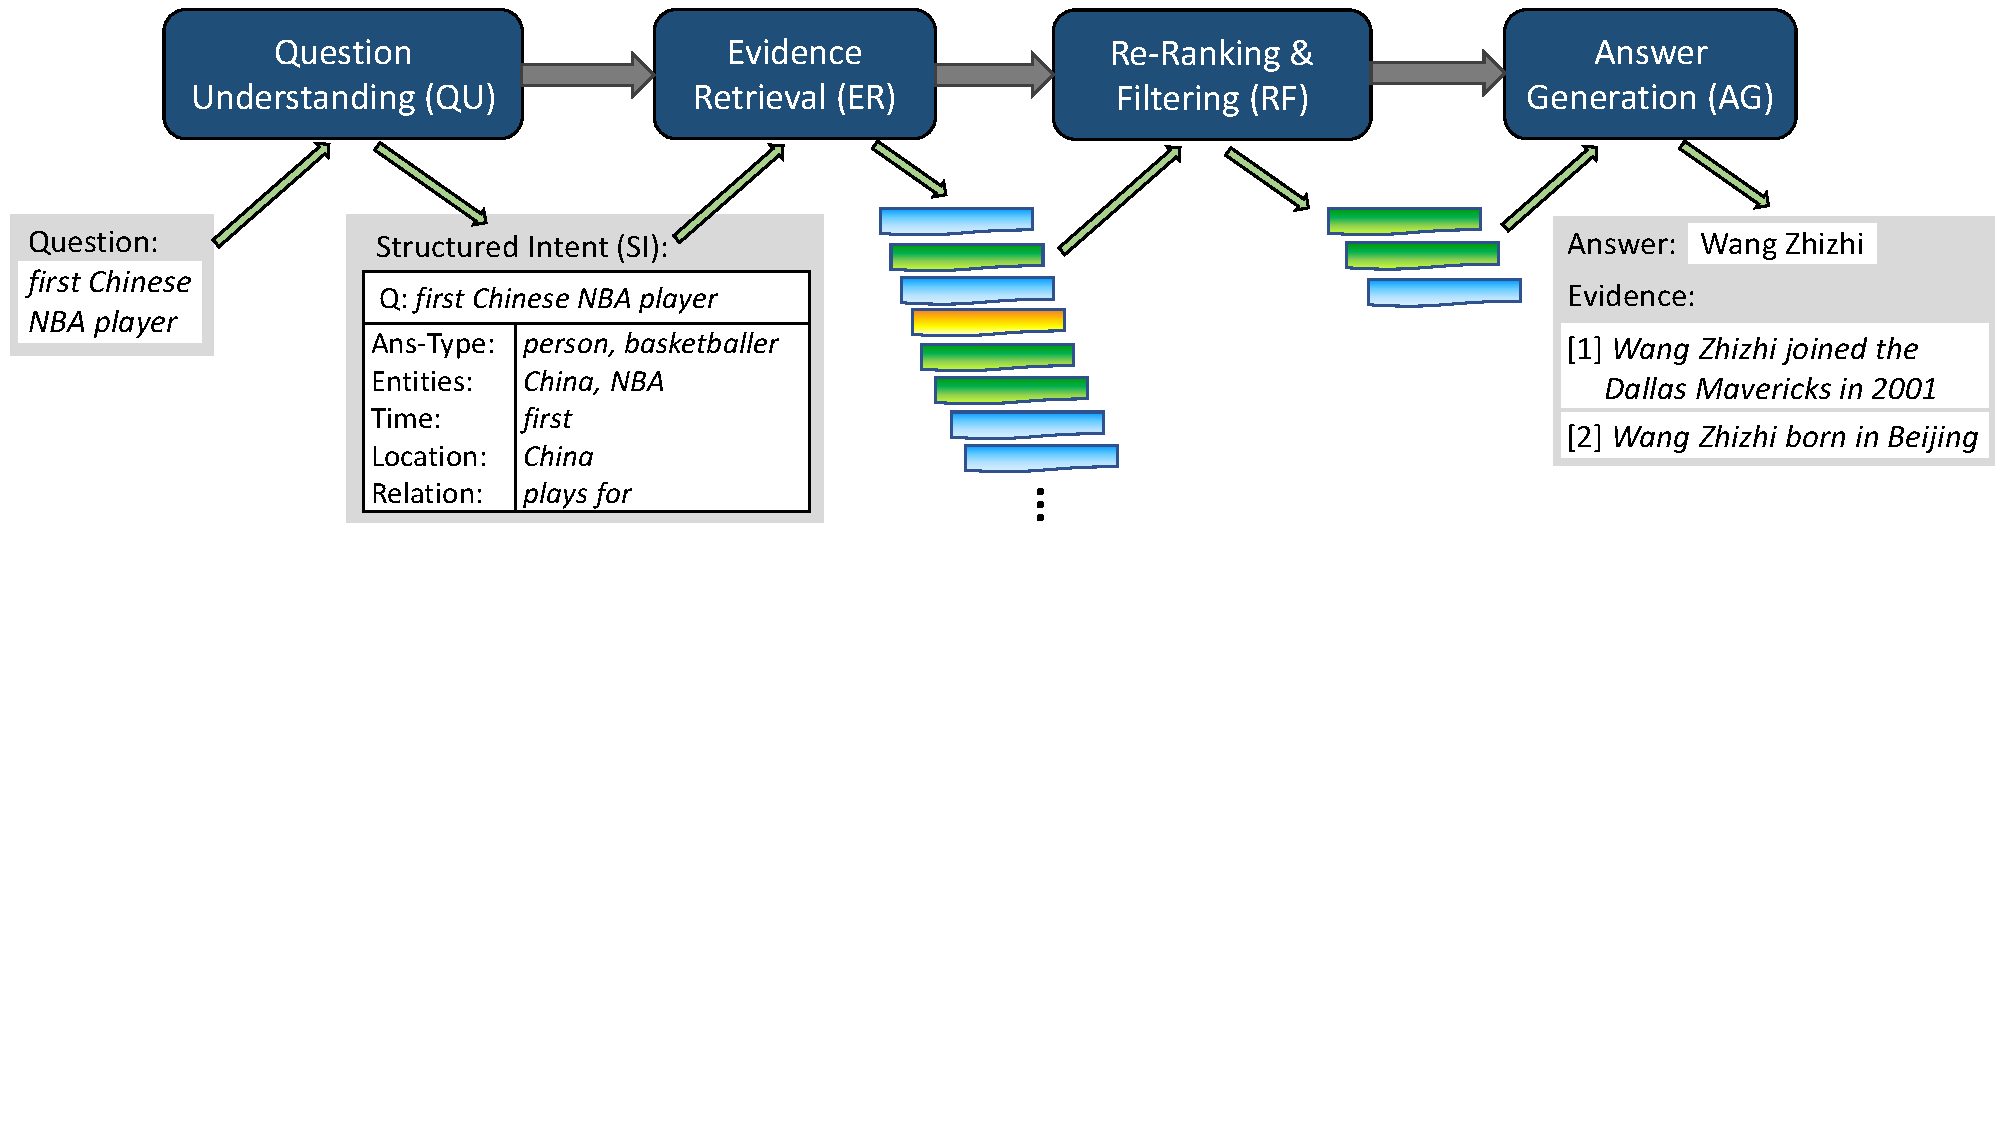
\includegraphics[width=\textwidth]{submissions/Gerhard2024/figures/compass-overview.pdf}
  \caption{Overview of the \method system.}
  \label{fig:compass-overview}
\end{figure}

% start with system overview
The \method system is a pipeline of four major stages, as illustrated in Figure \ref{fig:compass-overview}.
First, the input question is analyzed and decomposed, in order to compute a {\em structured intent (SI)} representation that will pass on to the subsequent steps, along with the original question. Second, the SI is utilized to retrieve pieces of evidence from different sources: text, KG and tables. 
Third, this pool of potentially useful evidence is filtered down, with iterative re-ranking, to arrive at a tractably small set of most promising evidence.
The final stage generates the answer from this evidence,
passing back the answer as well as evidence snippets for user-comprehensible explanation.

The second and fourth stage, Evidence Retrieval (ER) and Answer Generation (AG), are fairly standard. Such a two-phase architecture was called a retriever-reader architecture~\cite{Zhu-ODQA-survey:arxiv2021}. With a modern LLM replacing the earlier kinds of neural readers, this is the core of every RAG system~\cite{DBLP:journals/arXiv/abs-2312-10997}.

Stages 1 and 3 are unique elements of our architecture, judiciously introduced to improve both effectiveness (i.e., answer quality) and efficiency (i.e., computational cost).
Question Understanding (QU) provides the ER component with crisper and semantically refined input, and
the Re-Ranking \& Filtering (RF) stage is beneficial for
distilling the best evidence from the large pool of retrieved pieces.
The following subsections elaborate on the four stages of the pipeline, emphasizing the \method-specific steps QU and RF.



\subsection{Question Understanding (QU)}

% one par introducing the SI
To prepare the retrieval from different kinds of sources, including a KG, ad-hoc tables and text documents, it is useful to analyze and decompose the user question.
In this work, we aim to cast a question into a 
{\em structured intent (SI)} representation: essentially
a frame with faceted cues as slots, or equivalently, a concise set of key-value pairs. 
Figure \ref{fig:compass-overview} gives an idealized example for the question about the first Chinese NBA player. The facets or keys of potential interest here 
are:
\squishlist
\item {\em Ans-Type:} the expected answer type (or types when considering
different levels of semantic refinement), 
\item {\em Entities:} the salient entities in the question, and 
\item {\em Relation:} phrases that indicate which relation (between Q and A entities) the user is interested in. 
\squishend
\noindent In addition, as questions can have temporal or spatial aspects, the SI also foresees slots for:
\squishlist
\item {\em Time:} cues about answer-relevant time points or spans, including relative cues (e.g., ``before Covid'') and ordinal cues (e.g., ``first''), and
\item {\em Location:} cues about answer-relevant geo-locations.
\squishend

% discuss the spectrum of different SIs
\vspace{0.2cm}
\noindent The ideal SI for example question Q2 would look like:

\begin{quote}
{\em Ans-Type:} person, basketballer; {\em Entities:} China, NBA; {\em Time:} first;
{\em Location:} China; {\em Relation:} plays for.
\end{quote}

Note that the values for these slots can be crisp like entity names or dates, but they can also take the form of surface phrases. The SI purpose and value lie in the decomposition. In practice, many questions would only lead to a subset of faceted cues, leaving some slots empty. For the example in Figure \ref{fig:compass-overview}, an alternative SI could simply consist of

\begin{quote}
{\em Ans-Type:} person; {\em Entities:} China, NBA; {\em Time:} first.
\end{quote}

\noindent Even this simplified SI can be highly beneficial in guiding the subsequent evidence retrieval.

% sketch how an LM is trained to generate SIs 
To generate the SI from a user question, we employ a (small-scale) LM, specifically BART~\cite{DBLP:conf/acl/LewisLGGMLSZ20}, a Transformer-based auto-encoder with 140M parameters.\footnote{\url{https://huggingface.co/facebook/bart-base}}
BART is pre-trained for language representation; its power for our purpose comes from fine-tuning.
To this end, we generate (question, SI) pairs by using an instruction-trained LLM like GPT-4, with few-shot in-context learning (following our earlier work~\cite{Jia-FAITH:WWW2024}). 
Note that this is a one-time action; at inference-time we only use much smaller LMs.
The generated silver-standard pairs are then used to fine-tune BART.
In the experiments in this article, we leverage pre-existing collections of silver pairs, based on the training data of the CompMix benchmark~\cite{Christmann-CompMix:WWW2024}, 
comprising $3{,}400$ such pairs.


% outline value of SI for conversations
Although this paper focuses on single-shot questions, the \method architecture is also geared for conversational QA. In that setting, the SI can play an even bigger role, as (follow-up) questions are often formulated in a rather sloppy manner -- all but self-contained. For example, a conversation could start with a clear question {\em When did Wang Zhizhi join the NBA?}, followed a few dialog steps later, by a user utterance like {\em Which teams did he play for?} or simply {\em Which teams?}.
In such an informal conversation, the system needs to {\em contextualize} each user utterance based on the preceding turns in the dialog (e.g., inferring the relevant entities Wang Zhizhi and NBA from the conversational history).
For details on conversational QA, based on our architecture, see our earlier works~\cite{Christmann-CONVINSE:SIGIR2022,Christmann-Explaignn:SIGIR2023}.







%%%%%%%%%%%%%%%%%%%%%%%%%%%%%%%%%%%%%
\subsection{Evidence Retrieval (ER)}

The ER stage taps into a knowledge graph, a corpus of text documents, and a collection of web tables.
Specifically, for the experiments, we use the Wikidata KG,
all English Wikipedia articles, and all tables that are embedded in Wikipedia pages (incl. infoboxes, which can be seen as a special case of tables). 

% specifics: Clocq etc. - and the role of the SI
\vspace{0.2cm}
\noindent{\bf Retrieval from KG:}
To retrieve evidence from the KG, we utilize our earlier work
\clocq~\cite{Christmann-CLOCQ:WSDM2022}, which provides entity disambiguations and a relevant KG-subgraph for a given query.
Unlike most other works on QA-over-KG, \clocq fetches all KG-facts that are relevant for a given entity in a single step.
For example, when querying for
NBA players, it can traverse the KG neighborhood and pick up top teams, also considering so-called qualifier nodes in Wikidata which are often used for temporal scopes. 
As the disambiguation of entity names onto the KG can be tricky and noisy (e.g., China could be mapped to Chinese sports teams in all kinds of sports), \clocq considers several possible disambiguations~\cite{Christmann-CLOCQ:WSDM2022} (typically in the order of $10$ result entities).
The queries for \clocq are 
constructed by concatenating all slots of the question's SI.
For the example query about the first Chinese NBA player,
good result entities would be Dallas Mavericks, lists about NBA seasons, MVP awards etc., and their associated facts. These provide cues, but are likely insufficient to answer the question.


\vspace{0.2cm}
\noindent{\bf Retrieval from Text and Tables:}
The disambiguated entities returned by \clocq form anchors for tapping into text and tables.
\method first identifies 
relevant text documents and tables that refer to the anchor entities. With focus on Wikipedia, these are simply the articles for the respective entities. 
\method then constructs a keyword query that concatenates all available fields of the SI.
The query is evaluated against a linearized and verbalized representation (see below) of all sentences and all table rows in the selected documents.
This returns a set of sentences and 
and individual table rows, ranked by BM25 scores.


\vspace{0.2cm}
\noindent{\bf Evidence Verbalization:}
All results from the different data sources are uniformly treated by {\em linearizing} and {\em verbalizing} them
into token sequences. For KG results, the entity-centric triple sets are linearized via breadth-first traversal of the mini-graph starting from the entity node.
For tables, results are individual rows, which are contextualized by including labels from column headers and from the DOM-tree path of the article where the table comes from. For example, a table row about Wang Zhizhi playing for Dallas (Mavericks) in the 2000-2001 season, would be expressed as:

\vspace{0.05cm}
\hspace*{0.5cm} Wang Zhizhi / NBA Career / Season: 2000-2001, Team: Dallas, Games Played: 5 \dots
\vspace{0.05cm}

\noindent Finally, results from the text corpus are already in the form of token sequences, but we can additionally prefix these with the DOM-tree labels.
We can think of this entire pool of evidence as 
an on-the-fly corpus of potentially relevant pseudo-sentences, forming the input of the subsequent RF stage.


\vspace{0.2cm}
\noindent {\bf Result Ranking:}
Overall, the ER stage compiles a substantial set of evidence, possibly many thousands of entities, text snippets and table rows. Therefore, we practically restrict the pool to a subset of high-scoring pieces, like the top-$1000$.
For scoring, a simple BM25 model (a classical IR method) is applied. 
By default, we treat all evidence pieces uniformly with global scoring, no matter whether they come from KG, text or tables. 


\subsection{Re-Ranking and Filtering (RF)}

With a pool of top-$1000$ evidence pieces, we could invoke an LLM for answer generation. However, that would face a large fraction of noise (i.e., misleading evidence) and incur high costs of computation and energy consumption. 

For both of these reasons, we have devised light-weight techniques for iteratively reducing the top-$1000$ pieces to a small subset, say top-$30$ or top-$10$, that can be fed into an LLM at much lower cost (as LLM computations and pricing are at least linear in the number of input tokens). The difficulty is, of course, to do this without losing good evidence and reducing answer presence. Our techniques for this task are based on graph neural networks (GNNs)~\cite{Wu:IEEE2021} or cross-encoders (CEs)~\cite{Dejean:arxiv2024,Lin:MC2021}.

\myparagraph{GNN-based RF}
Given a large pool of evidence pieces from all sources, a bipartite graph is constructed:
\squishlist
\item {\em nodes} being evidence pieces or entities that occur in these pieces, and
\item {\em edges} connecting an evidence piece and an entity if the entity occurs in the evidence.
\squishend


The task for the GNN is to jointly score the evidence and the entity nodes in a multi-task learning setup. The latter are the {\em answer candidates}, and the evidence should give {\em faithful explanation} for an answer.
We build on our earlier work on explainable QA~\cite{Christmann-Explaignn:SIGIR2023}.

The node encodings are initialized with cross-encoder embeddings (see below) 
for node contents and the SI of the question. The inference iteratively adjusts the encodings based on message passing from neighboring nodes.
The GNN is trained via weak supervision from question-answer pairs:
evidence nodes are labeled as relevant if they are connected to
a gold answer.
More technical details are given in~\cite{Christmann-Explaignn:SIGIR2023}.

\method invokes the GNN in multiple rounds, iteratively reducing top-$k$ to top-$k^*$ nodes with $k^* \ll k$. In practice, we would typically consider two rounds: re-ranking top-$1000$ and pruning to top-100, and then reducing to top-30 or top-10, which are passed to the answer generation stage.
Note that this keeps the GNN at a tightly controlled size, so that its computational costs at inference-time are much smaller than those of an LLM.


\myparagraph{CE-based RF}
An alternative to the GNN inference is to employ a cross-encoder for scoring and re-ranking the evidence pieces.
These are transformers (typically with a small LM like BERT) that are fine-tuned for scoring the relatedness between a query and a document~\cite{Nogueira:arxiv2019}. In our case, the comparison is between the question SI and the evidence piece. In our experiments, we make use of two different cross-encoders, 
both trained on the MS-MARCO benchmark for passage retrieval~\cite{Bajaj:arxiv2018}, 
and fine-tuned on the respective benchmark (leveraging the same weak supervision data as for the GNNs),
the difference being in model size.\footnote{\url{https://huggingface.co/cross-encoder/ms-marco-MiniLM-L-4-v2} and\\ \url{https://huggingface.co/cross-encoder/ms-marco-MiniLM-L-6-v2}}
We use the smaller model to reduce top-$1000$ to top-100, and the larger model to go further down from top-100 to top-30.




%%%%%%%%%%%%%%%%%%%%%%%%%%%%%%%%%%%%%

\subsection{Answer Generation (AG)}

The last stage follows mainstream practice to invoke an LLM in a retrieval-augmented manner.
We call a `small-scale` LLM, specifically a fine-tuned LlaMA-3.1 model (8B-Instruct)\footnote{\url{https://huggingface.co/meta-llama/Llama-3.1-8B-Instruct}}, with a prompt \footnote{The specific prompt is \phrase{SI: \textless\texttt{concatenated SI}\textgreater \hspace{0.1cm} Evidence: \textless\texttt{evidence pieces}\textgreater}.}
consisting of:

\squishlist
\item the concatenated SI of the original question, and
\item the top-30 (or other top-$k^*$ with small $k^*$) evidence pieces.
\squishend

By the previous down-filtering of the original pool of evidence pieces, this last step has affordable cost in terms of computation time and energy consumption.

\vspace{0.2cm}
\noindent{\bf Fine-Tuning the LLM:}
We considered adding an instruction to the prompting, such as {\em ``answer this question solely based on the provided evidence snippets''}.
However, this turned out to be ineffective.
The reason why the model works well without such instructions is our task-specific fine-tuning.
We perform this by running the training data of benchmarks through the \method pipeline,
and training the AG stage with the top-30 evidence pieces as input.
Thus, the fine-tuning makes the model learn the role of evidence for RAG-based QA.

\vspace{0.2cm}
\noindent{\bf Explanations:}
The top-30 evidence pieces can be used to provide users with explanation of answers.
Optionally, these could be reduced further for comprehensibility.
Alternatively, we can fine-tune the LLM to provide both answers and concise explanations.
Since we can infer which evidences in the input mention the annotated ground-truth answers,
our method could be fine-tuned to provide such \textit{answering evidences} as well (cf.~\cite{Gao-citations:emnlp2023}).

\label{sec:exp}
\section{Experiments}


\label{setup}
\subsection{Experimental setup}


%%% BENCHMARKS
\myparagraphnospace{Benchmarks} We run experiments on three benchmarks with different characteristics of questions.

\squishlist
    \item \textbf{\compmix}.
    \compmix~\cite{Christmann-CompMix:WWW2024} is a benchmark which was specifically designed for evaluating QA systems operating over heterogeneous sources. The dataset has $9{,}410$ questions, out of which $2{,}764$ are used for testing.
    Answers are crisp entity names, dates, or other literals.
    
    \item \textbf{\crag}.
    We further evaluate on a subset of the \crag~\cite{Yang-CRAG} dataset, which was recently released as a testbed for RAG-based QA systems.
    We utilize the same pipeline and sources as outlined in Section~\ref{sec:method}, without using the web snippets or APIs provided with \crag. This way we focus on entity-centric questions that do not require access to live web data (e.g., news feeds), and disregard cases where the results would be up-to-date quantities.
    This restricts the test data to $436$ entity-centric questions, still enough for a proof of concept.
    
    \item \textbf{\timequestions}.
    To showcase the generalizability of our pipeline, we conduct experiments on~\timequestions~\cite{Jia-TimeQuestions},
    a benchmark for temporal QA. The dataset requires temporal understanding and reasoning, which are well-known limitations of
    LLMs~\cite{Dhingra-time-aware-LLM:TACL2022}. \timequestions has 16{,}181 questions (3{,}237 for testing).
\squishend

Typical examples for the questions in these three benchmarks are:

\begin{quote}
\compmix: \utterance{Which player won the most number of Man-of-the-Match titles in the FIFA world cup of 2006?}\\
 \indent \crag: \utterance{What was the worldwide box office sales for little hercules?}\\ 
  \indent \timequestions: \utterance{Which club did Cristiano Ronaldo play for before joining Real Madrid?}
\end{quote}

%%% BASELINES
\myparagraph{Baselines} As competitors or reference points to \method, we study the performance of the following methods:

\squishlist
    \item \textbf{Generative LLMs}.
    We compare \method against out-of-the-box LLMs: \textbf{\gptthree} (\texttt{text-davinci-003}), \textbf{\gptfour} (\texttt{gpt-4}) 
    and \textbf{\llama} (\texttt{meta-llama/Llama-3.1-8B-Instruct}).
    The same prompt is used for all LLMs, consistent with previous work~\cite{Christmann-CompMix:WWW2024, Zhang-Spaghetti:ACL2024}:
    \phrase{Please answer the following question by providing the crisp answer entity, date, year, or numeric number. Q: \textless\texttt{question}\textgreater}.
    

    \item \textbf{Heterogeneous QA methods}.
    \convinse~\cite{Christmann-CONVINSE:SIGIR2022}, \unikqa~\cite{Oguz-UniK-QA:NAACL2022}, \explaignn~\cite{Christmann-Explaignn:SIGIR2023}
    are QA methods designed to integrate heterogeneous sources: text, tables and KG. All of these  integrate the exact same sources as \method.

    
    \item \textbf{\textsc{State-of-the-art}}.
    For \compmix and \timequestions, we also compare against state-of-the-art methods from the literature: \spaghetti~\cite{Zhang-Spaghetti:ACL2024} and \textsc{Un-Faith}~\cite{Jia-FAITH:WWW2024}, which are among the best performing systems.
    
Results are taken from the literature whenever applicable.
On \crag, we use the models trained on \compmix for \method and heterogeneous QA baselines.
\squishend



%%% METRIC(S)
\myparagraph{Metrics}
We measure \textit{precision at 1} (\textbf{P@1}) as our main metric~\cite{RoyAnand:MC2021} on all benchmarks.
On \crag, we manually annotate answer correctness, as the ground-truth answer formats vary (e.g., entity name variants, lists, sentences).

We also compute the number of neural parameters aggregated over all sub-modules (\textbf{\#Parameters}).
Parameter counts for GPT-models are taken from~\cite{Minaee-LLM-survey}
(\gptfour might have less active parameters during inference).

For further analysis we measure \textit{answer presence} (\textbf{AP@k}),
i.e. whether the answer is present in the top-$k$ ranked evidence pieces,
and \textit{mean reciprocal rank} within the top-$k$ evidences (\textbf{MRR@k}).

%%% CONFIG
\myparagraph{Configuration}
Our implementation uses the \texttt{Llama3.1-8B-Instruct} model for the AG stage.
For the QU, ER and RF stages
we adopt code from the \explaignn project.\footnote{\url{https://explaignn.mpi-inf.mpg.de}}
For the ER stage, we use \clocq, setting its specific parameters to $k=10$ and $p=1{,}000$.

As default, we use the GNN technique for the RF stage.
For efficiency, we use light-weight models for initializing
the GNN encoders -- the same models used for the CE-based RF.\footnote{\url{https://huggingface.co/cross-encoder/ms-marco-MiniLM-L-4-v2} and\\\url{https://huggingface.co/cross-encoder/ms-marco-MiniLM-L-6-v2}}
The GNNs are trained for $5$ epochs with an epoch-wise evaluation strategy,
i.e. we choose the model with the best performance on the respective dev set.
We train the GNNs on graphs with a maximum of $100$ evidence and $400$ entity nodes (as scored by BM25).
During inference, the first GNN is applied on graphs with $1{,}000$ evidence and $4{,}000$ entity nodes, shrinking the pool of evidence pieces to the top-$100$.
The second GNN then runs on graphs with $100$ evidence and $400$ entity nodes.
The factor of 4 entities per evidence (on average) holds sufficient for the observed data,
and enables batched inference.
Other parameters are kept as is.

The AG model, based on \texttt{Llama3.1-8B-Instruct}, is 
fine-tuned
for $2$ epochs with a warm-up ratio of $0.01$ and a batch size of $8$, again with an epoch-wise evaluation strategy.
Other parameters are set to the default Hugging Face
training parameters.\footnote{\url{https://huggingface.co/docs/transformers/v4.46.2/en/main_classes/trainer\#transformers.TrainingArguments}}





\subsection{Main results}
%%% MAIN TABLE
\myparagraphnospace{\method is competitive on all benchmarks}
Main results of our experiments are shown in Table~\ref{tab:main-res}.
First of all, we note that \method achieves competitive performance across all three benchmarks.

On \compmix, baselines for heterogeneous QA and \llama perform similarly,
whereas GPT-based LLMs can answer more than $50$\% of the questions correctly.
\method exhibits substantially higher performance, on par with
the state-of-the-art method \textsc{Spaghetti}~\cite{Zhang-Spaghetti:ACL2024}
(which is based on \gptfour).

On the \crag dataset, P@1 drops for all methods except for \gptfour. 
The benchmark includes realistic questions,
which can be ambiguous/confusing (\phrase{who was the director for the report?}),
on ``exotic'' entities with answers in social media (\phrase{how many members does the teknoist have?}),
or require up-to-date information (\phrase{when did chris brown release a song or album the last time?}),
and other cases that are challenging for all methods.

Finally, \method establishes new state-of-the-art performance on the \timequestions benchmark.
Interestingly, all of the tested LLMs show greatly reduced performance on this benchmark,
which inherently requires temporal understanding and reasoning
-- a known weakness of stand-alone LLMs.


\begin{table} [h]
    \centering
    \newcolumntype{G}{>{\columncolor [gray] {0.90}}c}
    \begin{tabular}{l G G G c}
        \toprule
            \textbf{Method $\downarrow$ / Benchmark $\rightarrow$} & \textbf{\compmix}  & \textbf{\crag} & \textbf{\timequestions} & \textbf{\#Parameters} \\ 
        \midrule
            \textbf{\gptthree} 
            & $0.502$ &   $-$ & $0.224$ & $175{,}000$ M  \\
            % #params from https://arxiv.org/pdf/2402.06196

            \textbf{\gptfour}
            & $0.528$ &   $\mathbf{0.633}$ & $0.306$ & $1{,}760{,}000$ M \\
            % #params from https://arxiv.org/pdf/2402.06196

            \textbf{\llama~\cite{Touvron-LLaMA}} (8B-Instruct)
            & $0.431$ &   $0.385$ & $0.178$ & $8{,}030$ M  \\
            % #params from Huggingface (8,030,257,152)
        \midrule
            \textbf{\convinse~\cite{Christmann-CONVINSE:SIGIR2022}}
            & $0.407$  &   $0.298$ & $0.423$  & $362$ M \\
            % FiD: 222,903,936 + BART (SR-generation): 139,420,416 = 362,324,352 (python explaignn/question_understanding/structured_representation/get_num_params.py)

            \textbf{\unikqa~\cite{Oguz-UniK-QA:NAACL2022}}
            & $0.440$ &   $0.280$ & $0.424$ & $223$ M  \\
            % FiD: 222,903,936 (python explaignn/heterogeneous_answering/fid_module/FiD/get_num_params.py)
    
            \textbf{\explaignn~\cite{Christmann-Explaignn:SIGIR2023}} 
            & $0.442$ &   $0.303$ & $0.525$  & $328$ M \\
            % BART (SR-generation): 139,420,416 + 2GNNs: 94520832 + 93930240 = 327,871,488

        \midrule 
            \textbf{\textsc{State-of-the-art}}
            & $\mathbf{0.565}$ 
            & $-$
            & $0.571$  & $-$ \\

            & (\textsc{Spaghetti}~\cite{Zhang-Spaghetti:ACL2024})
            & 
            & (\textsc{Un-Faith}~\cite{Jia-FAITH:WWW2024}) &  \\

        \midrule
            \textbf{\method (ours)}
            & ${0.564}$ &   $0.362$ & $\mathbf{0.754}$  & $8{,}218$ M \\
            % BART (SR-generation): 139,420,416 + LLaMA: 8,030,257,152 + GNNs: 25,670,016 + 22,268,928 =  8,217,616,510
        \bottomrule
    \end{tabular} 
    \vspace*{-0.2cm}
    \caption{End-to-end P@1 of \method and baselines on three benchmarks. Results for \gptthree and \gptfour are taken from the literature~\cite{Christmann-CompMix:WWW2024, Jia-FAITH:WWW2024}. \gptthree is not accessible anymore, hence no results on \crag.
    }
    \label{tab:main-res}
\end{table}





%%% ANSWER SOURCES
\myparagraph{Integration of heterogeneous sources is vital}
\method integrates evidence from text, KG and tables into a unified framework.
We aim to better understand how this affects the answering performance of the method.
Table~\ref{tab:sources} shows end-to-end answering performance of \method
with different combinations of the input sources.
The results clearly indicate that all types of sources contribute, with option Text+KG+Tables performing best,
with a large margin over tapping only single source types.

\begin{table} [t] 
    \centering
    \newcolumntype{G}{>{\columncolor [gray] {0.90}}c}
    \newcolumntype{H}{>{\setbox0=\hbox\bgroup}c<{\egroup}@{}}
    	\begin{tabular}{l G G G H H H c c c} 
        \toprule
            \textbf{Benchmark $\rightarrow$}
                & \multicolumn{3}{G}{\textbf{\compmix}} 
                & \multicolumn{3}{H}{\textbf{\crag}}
                & \multicolumn{3}{c}{\textbf{\timequestions}} \\ 
        \midrule
            \textbf{Input sources $\downarrow$ / Metric $\rightarrow$}
                & \textbf{P@1} & \textbf{AP@100}  & \textbf{AP@30}
                & \textbf{P@1} & \textbf{AP@100}  & \textbf{AP@30}
                & \textbf{P@1} & \textbf{AP@100}  & \textbf{AP@30} \\
            \midrule
                \textbf{Text}           &  $0.455$  &  $0.563$  &  $0.531$ &  $?$  &  $?$  &  $?$ &  $0.539$  &  $0.515$  &  $0.487$   \\
                \textbf{KG}             &  $0.481$  &  $0.677$  &  $0.637$ &  $?$  &  $?$  &  $?$ &  $0.724$  &  $0.701$  &  $0.674$   \\
                \textbf{Tables}         &  $0.432$  &  $0.501$  &  $0.482$ &  $?$  &  $?$  &  $?$ &  $0.536$  &  $0.347$  &  $0.328$   \\
            \midrule
                \textbf{Text+KG}        &  $0.537$  &  $0.749$  &  $0.706$ &  $?$  &  $?$  &  $?$ &  $0.745$  &  $\mathbf{0.776}$  &  $0.748$   \\
                \textbf{Text+Tables}    &  $0.503$  &  $0.632$  &  $0.594$ &  $?$  &  $?$  &  $?$ &  $0.567$  &  $0.578$  &  $0.549$   \\
                \textbf{KG+Tables}      &  $0.524$  &  $0.728$  &  $0.692$ &  $?$  &  $?$  &  $?$ &  $ 0.743$  &  $0.731$  &  $0.703$   \\
            \midrule
                \textbf{Text+KG+Tables}    &  $\mathbf{0.564}$  &  $\mathbf{0.759}$  &  $\mathbf{0.724}$ &  $?$ &  $?$  &  $?$ & $\mathbf{0.754}$    & $\mathbf{0.776}$  &  $\mathbf{0.749}$   \\
            \bottomrule
    \end{tabular}
    \vspace*{-0.2cm}
    \caption{Answer presence and answering precision of \method with different combinations of input sources (on the respective test sets).}
    \label{tab:sources}
\end{table}




\subsection{Analysis}

%%% TOP-K vs. 3xTOP-(K/3)
\myparagraph{Unified retrieval enhances performance}
In the RF stage, we re-rank and filter evidence from different source types,
and feed the unified top-\textit{k}* into the AG stage.
We conduct a comparison in which we consider
the top-$10$ evidence pieces from each source type individually. This gives equal influence to KG, text and tables, whereas our default is based on global ranking.
Table~\ref{tab:unified-retrieval} shows the results for this analysis, showing our default choice performs better.
The reason is that different questions require different amounts of evidence from each of the source types.

\begin{table} [t] 
    \centering
    \newcolumntype{G}{>{\columncolor [gray] {0.90}}c}
    \newcolumntype{H}{>{\setbox0=\hbox\bgroup}c<{\egroup}@{}}
    	\begin{tabular}{l G G H H} 
        \toprule
            \textbf{Input evidences $\downarrow$ / Metric $\rightarrow$} & \textbf{P@1} & \textbf{AP@30}  & \textbf{\crag} & \textbf{\timequestions} \\ 
            \midrule
                \textbf{Top-30 Text+KG+Tables (ours)}             &  $\mathbf{0.574}$  &  $\mathbf{0.710}$  &  $-$  &  $-$   \\
                \textbf{Top-10 Text + Top-10 KG + Top-10 Tables}        &  $0.560$    &  $0.709$  &  $-$  &  $-$   \\
            \bottomrule
    \end{tabular}
    \vspace*{-0.2cm}
    \caption{Answer presence and precision
    of \method for different choices of top-30 
    (on \compmix dev set).}
    \label{tab:unified-retrieval}
\end{table}


%%% NUMBER OF EVIDENCES
\myparagraph{\method works well with small amounts of evidence}
We investigate the 
influence of 
the number of evidence pieces
fed into the AG stage, varying it from $5$ to $100$.
Results are shown in Figure~\ref{fig:res-num-evidences}.
As the curve shows, there is a sharp increase in precision as we add evidence up to 30 or 40 pieces, which is around our default of top-30. This indicates that a certain amount of evidence is needed, to overcome the inherent noise and arrive at sufficient answer presence. 
As we increase the amount of evidence further, we observe a saturation effect, and eventually a degration of performance. Too much evidence not only has diminishing returns, but can actually be confusing for the AG stage. This reconfirms our heuristic choice of top-30: enough for good answering while keeping computational costs reasonably low.


\begin{figure}[t]
    \centering
    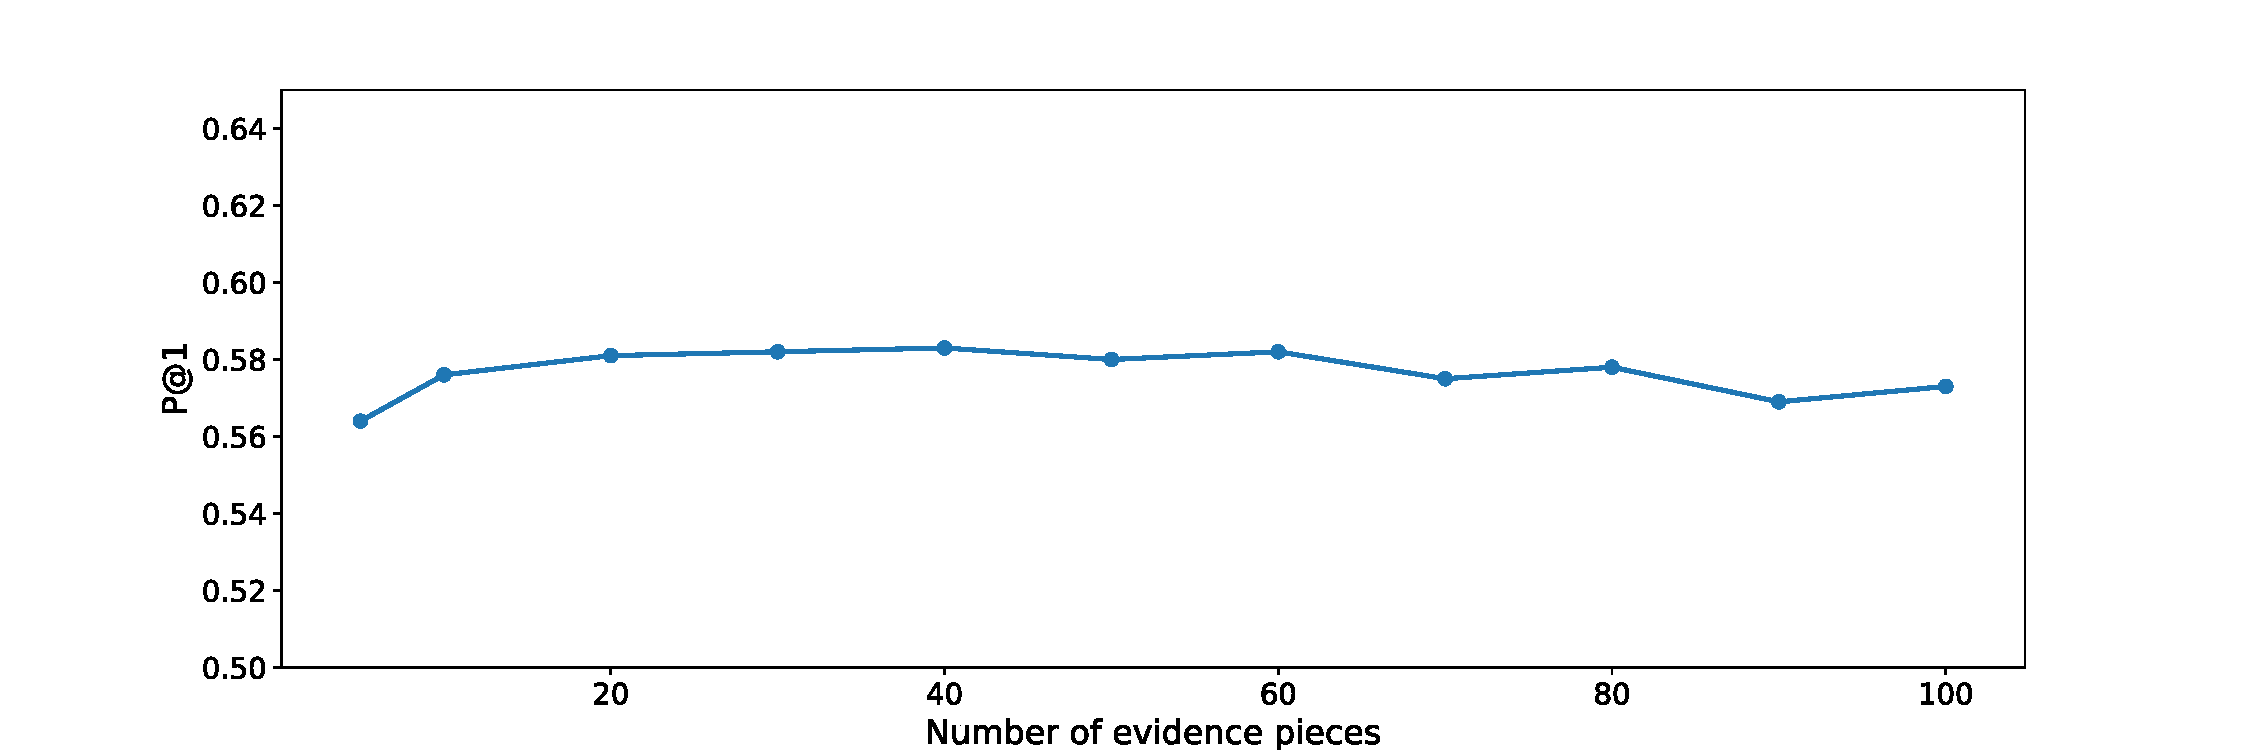
\includegraphics[width=0.8\textwidth]{submissions/Gerhard2024/figures/p_at_1-line_with_evidences.pdf}
    \vspace*{-0.2cm}
    \caption{Performance of \method on the \compmix dev set with different numbers of evidence.}
    \label{fig:res-num-evidences}
    \vspace*{-0.2cm}
\end{figure}



%%% ABLATION
\myparagraph{Ablation study on re-ranking} For more insight on the possible configurations of the RF stage, we conducted an ablation study with different options, including solely relying on the initial BM25 scoring without explicit re-ranking. The results are shown in Table \ref{tab:ablation2}. We observe that the iterative reduction in two steps is slightly better than the single-step variants (going down from top-1000 to top-30 in one RF step). Between the two options of using a GNN or a CE, the differences are negligible. A notable effect is that our RF techniques retain the answer presence at a very high level, only a bit lower than for the initial top-1000. 
The last two rows of Table \ref{tab:ablation2} demonstrate that RF is crucial: without explicit re-ranking, the technique of just picking smaller top-$k$ from the original BM25 model leads to substantial degradation in both answer presence and precision. 


\begin{table} [t] \small
    \centering
    \newcolumntype{G}{>{\columncolor [gray] {0.90}}c}
    \newcolumntype{H}{>{\setbox0=\hbox\bgroup}c<{\egroup}@{}}
    	\begin{tabular}{l G H G G G} 
        \toprule
            & \multicolumn{5}{G}{\textbf{\compmix} (dev set)} \\
        \midrule
            \textbf{RF Method $\downarrow$ / Metric $\rightarrow$} & \textbf{P@1} & \textbf{AP@1000} & \textbf{AP@100}  & \textbf{AP@30} & \textbf{MRR@100} \\ 
        \midrule
            \textbf{GNN: 1000 $\rightarrow$ 100 $\rightarrow$ 30}             &  $\mathbf{0.574}$  & $0.760$ &  $0.738$  &  $0.710$  &  $\mathbf{0.572}$  \\
            \textbf{CE: 1000 $\rightarrow$ 100 $\rightarrow$ 30}          &  $0.573$  & $0.760$  &   $\mathbf{0.740}$ &  $\mathbf{0.721}$   &  $0.553$   \\
        \midrule
            \textbf{GNN: 1000 $\rightarrow$ 30} &  $0.567$  & $?$  &   $n/a$ &  $0.710$   &  $0.567$   \\
         \textbf{CE: 1000 $\rightarrow$ 30} &  $0.570$  & $0.760$  &   $n/a$ &  $0.715$   &  $0.558$   \\
            \midrule
           \textbf{BM25: 100 (w/o GNN or CE)} &  $0.490$ & $0.760$  &  $0.652$  &  $n/a$  &  $0.259$ \\       
            \textbf{BM25: 30 (w/o GNN or CE)} &  $0.468$  & $0.760$  &  $n/a$ &  $0.534$   &  $0.259$   \\
            \bottomrule
    \end{tabular}
    \vspace*{-0.2cm}
    \caption{Ablation study for different RF strategies of \method on the \compmix dev set. The answer presence in the RF input with top-$1000$ evidence pieces is $0.760$.}
    \label{tab:ablation2}
\end{table}



\myparagraph{Quality of SI}
To assess the quality and robustness of the Structured Intents, we
inspected a sample of questions and their SIs.
Table~\ref{tab:question-SI-examples} gives three anecdotic examples.
We show SIs generated by \method, which makes use of the pre-existing collection from the \compmix benchmark for training.
This training data was obtained via different heuristics, 
which can be a limiting factor when user intents become more complex.

Therefore, we also looked at SIs derived via in-context learning (ICL) using \gptfour with $5$ handcrafted examples.
As shown in our earlier work on temporal QA~\cite{Jia-FAITH:WWW2024},
such data can be used for training smaller models (e.g., BART),
which can greatly boost the completeness and overall quality of the generated SIs.

From the sampled set, we observed that the ICL-based SIs are more
complete with all slots filled, whereas the BART-based SIs focused more
on the main slots Answer-type, Entities and Relation.
However, both approaches achieve very high quality in filling the slots,
capturing the user's information need very well.

Interestingly, when questions get complicated, with nested phrases, 
the ICL-based variant succeeds in decomposing the questions, based on only $5$ ICL examples.
For example, for the question {\em ``which German state had the most Corona-related death cases in the first year after the outbreak?''}
the Time slot becomes {\em ``first year after Corona outbreak''},
which can be resolved to identify the temporal scope.
In general, we believe that such question decomposition, beyond simple temporal constraints,
would be an interesting theme for future work.

\begin{table} [t] 
    \centering
    \small
    \newcolumntype{G}{>{\columncolor [gray] {0.90}}c}
    \newcolumntype{H}{>{\setbox0=\hbox\bgroup}c<{\egroup}@{}}
    \resizebox*{\textwidth}{!}{
        \begin{tabular}{p{6cm}|p{6cm}|p{6cm}} 
        \toprule
            \textbf{Question} & \textbf{Current SI by \method} & \textbf{SI via ICL} \\
        \midrule
        \textit{what was disneys first color movie?}
            & Ans-Type: \textit{animated feature film} & Ans-Type: \textit{film, animated film} \\
            & Entities: \textit{disneys} & Entities: \textit{Disney} \\
            & Relation: \textit{was first color movie} & Relation: \textit{first color movie} \\
            &  & Time: \textit{first} \\
        \midrule
        \textit{at the oscars, who won best actor in 2018?}
            & Ans-Type: \textit{human} & Ans-Type: \textit{person, actor} \\
            & Entities: \textit{at the oscars} & Entities: \textit{Oscars, 2018} \\
            & Relation: \textit{who won best actor in 2018} & Relation: \textit{won best actor} \\
            &  & Time: \textit{2018} \\
        \midrule
        \textit{which German state had the most Corona-} & Ans-Type: \textit{state} & Ans-Type: \textit{location, state} \\
        \textit{related death cases in the first year after} & Entities: \textit{Germany, Corona} & Entities: \textit{Germany, Corona-related deaths} \\
        \textit{the outbreak?} & Relation: \textit{which state had the most related} & Relation: \textit{highest count of death cases} \\
        & \textit{death cases in the first year after the out-}  & Location: \textit{Germany} \\
            & \textit{break}  & Time: \textit{first year after Corona outbreak} \\
        \bottomrule
    \end{tabular}
    }
    \vspace*{-0.2cm}
    \caption{Examples for pairs of question and generated SI.}
    \label{tab:question-SI-examples}
\end{table}




%%% REFRAIN FROM ANSWER
\myparagraph{Refraining from answering}
%%% Searched for: "generated_answer I" (with I being the full word, not partial) in the generated answers of LLaMA
%%% yields 245 results out of 2764 questions on CompMix
%%% yields 1270 results out of 3237 questions on TimeQuestions
We can train our model to refrain from answering in scenarios
where the provided evidence does not contain an answer to the question.
Specifically, during training, when the answer is not present in the evidence,
we change the target answer to {\em unknown}. This variant is referred to as \method {\em (faithful)}.

We measure the ratio of questions for which {\em unknown} is provided as answer,
and the P@1 restricted to questions that are answered.
The accuracy of refraining from answering is measured as well,
based on whether the answer is present in the evidence or not.
We conduct this experiment on \compmix and \timequestions,
for which we can compute answer presence exactly.
We also compute results for \llama, which is already instructed 
with the option to answer ``don't know''.
Table~\ref{tab:refrain-from-answer} shows the results.
For \compmix, we observe that \method has high accuracy on refraining when appropriate,
whereas \llama tends to be overconfident with a very small rate of {\em unknowns}, leading to incorrect answers.

\begin{table} [t] \small
    \centering
    \newcolumntype{G}{>{\columncolor [gray] {0.90}}c}
    \newcolumntype{H}{>{\setbox0=\hbox\bgroup}c<{\egroup}@{}}
    	\begin{tabular}{l G G G G c c c c} 
        \toprule
            & \multicolumn{4}{G}{\textbf{\compmix}} & \multicolumn{4}{c}{\textbf{\timequestions}} \\
            \midrule
            \textbf{Metric $\rightarrow$} & \textbf{P@1}  & \textbf{P@1} & \textbf{Refrain} & \textbf{Refrain} & \textbf{P@1}  & \textbf{P@1} & \textbf{Refrain} & \textbf{Refrain} \\ 
            \textbf{Method $\downarrow$} &                 & \textbf{(answered)} & \textbf{rate} & \textbf{accuracy} &                 & \textbf{(answered)} & \textbf{rate} & \textbf{accuracy} \\ 
            \midrule
                \textbf{\llama}             &  $0.431$  &  $0.471$  &  $0.089$  &  $n/a$  &  $0.177$  &  $0.276$  &  $0.392$  &  $n/a$  \\
                \textbf{\method (faithful)}           &  $0.497$  &  $0.713$  &  $0.303$  &  $0.838$ &  $0.597$  &  $0.804$  &  $0.257$  &  $0.864$  \\
            \bottomrule
    \end{tabular}
    \vspace*{-0.2cm}
    \caption{
        Performance of \method with option to refrain from answering (``don't know'').
    }
    \label{tab:refrain-from-answer}
\end{table}

\label{sec:disc}
\section{Insights, Limitations, and Challenges}


\noindent{\bf Benchmark Performance.} Our method, RAG-based \method with an 8B LLaMA model, outperforms much larger LLMs like \gptfour on two of the three benchmarks, with a very large margin for temporal questions. Obviously, pre-trained LLMs have only limited sense of properly positioning ``remembered’’ facts on the timeline even with training data that exceeds ours by several orders of magnitude. This confirms our intuition that LLMs alone are not good at ``recalling’’  higher-arity relations that require combining distant pieces of evidence. This is a sweet spot for RAG. Only for 
the \crag benchmark, \method is substantially inferior to a full-blown LLM. This is likely due to the nature of the questions: not necessarily the complexity of the information needs, but the need for more web sources (beyond what our experiments tap into).

\vspace{0.2cm}
\noindent{\bf Cost/Performance Ratio.} The most important take-away from our experiments is that \method achieves its competitive performance at a much lower cost than the full LLMs. Assuming that the consumed GFlops are proportional to the number of model parameters, \method achieves a cost reduction by a factor of 200x for \gptthree and 2000x for \gptfour. This does not only mean less computation, but also a massively lower electricity bill and climate impact.  

\vspace{0.2cm}
\noindent{\bf Role of Question Understanding.} We did not systematically investigate the influence of the Structured Intent in the \method pipeline. However, the comparison to the big GPT models reflects the role of the SI, as we prompt the GPT models in their natural mode with the original questions. The linearized sequence of available SI slots does not always have major advantages, but there are enough cases where specific facets provide crucial cues. This holds especially for the Entities slot, as this drives the gathering of evidence in the ER stage (cf.~\cite{Christmann-CONVINSE:SIGIR2022}, and for the Time slot, as these cues are often decisive for temporal questions (cf.~\cite{Jia-FAITH:WWW2024}).

\vspace{0.2cm}
\noindent{\bf Role of Re-Ranking.} As our ablation studies show, merely using top-$k$ evidence from an initial BM25-style ranking does not provide good performance. Also, there seems to be sweet spot in the choice of $k$: we need enough evidence for connecting the dots if the question requires multiple pieces of information, or for corroborating candidates if the question finds many useful but noisy pieces. In the experiments, $k=30$ turns out to be good choice; much lower $k$ results in insufficient evidence, and much larger $k$ leads to saturation and ultimately degrading performance. Our argument for iteratively shrinking the candidate set in multiple rounds of re-ranking is substantiated in our experiments, but the gain of doing this, compared to GNN- or CE-based re-ranking from 1000 to 30, is not big. More research is called to better understand the role of ranking in RAG. 

\vspace{0.2cm}
\noindent{\bf Limitations of Evidence Retrieval.}
For ER, we adopted more or less standard techniques. The results showed very good answer presence, in the order of 75\% in the top-100 or even top-30. An important case where this is insufficient are questions that require aggregating information over a large number of evidence pieces. An example is asking for the life-time total of 3-point scores of the basketball player Dirk Nowitzki.
This requires collecting a set of per-season tables with NBA player statistics, but also other web sources with numbers for his career before he joined the NBA (including his youth teams).
Of course, there are sometimes shortcuts like a Wikipedia article or biography mentioning the total number, but this cannot be universally assumed. The bottom line is that ER should be reconsidered as well, striving to improve the recall dimension.

\vspace{0.2cm}
\noindent{\bf Limitations of Answer Generation.}
For AG, we simply rely on a LLM,
using it as an extractor (``reader'') from the given evidence. Despite the wide belief that LLMs can perform deep
reasoning over many pieces of evidence, our experience is that the extraction works only well – robustly and faithfully – for relatively simple questions with a few multi-hop joins or simple aggregation over a few pieces. However, complicated questions such as asking for the top-100 NBA players with the largest number of life-time 3-point scores (again including their pre-NBA careers) are currently out of scope and will likely remain so for quite some time. This offers many opportunities for pushing the envelope further.

\vspace{0.2cm}
\noindent{\bf Trust in Data Sources.}
In our experiments, we considered all heterogeneous sources as trustworthy and unbiased. With focus on Wikidata and Wikipedia, this assumption has been well justified. In the wild, however, input data for RAG-based systems likely exhibit a wide spectrum of quality issues, in terms of stale information, biased positions, or simply false statements. Identifying trustworthy and up-to-date evidence and dealing with conflicting data, has been explored in other contexts (e.g., for KG curation~\cite{Dong-Trust:PVLDB2015}), but remains a major challenge for RAG-based QA.


\vspace{0.2cm}
\noindent{\bf Open Challenges and Future Work.} The best-performing methods in our experiment, mostly \method, reach P@1 values of 56\% for \compmix and 75\% for \timequestions. 
For the latter, the answer presence in the top-100 is only slightly higher; so the AG stage hardly misses anything.
However, for \compmix, the answer presence is 75\% -- much higher than what our system can actually answer. Obviously, closing this gap is a major direction to pursue, with focus on the RF and AG stages. However, missing one fourth of the answers completely in the top-100 pool, is a big problem as well. This requires improving recall at the ER stage, possibly with better guidance by the QU, which in turn needs more sources beyond the scope of our experiments (currently limited to Wikidata and Wikipedia). 

In general, we need to think beyond this kind of ``benchmark mindset’’. Even if we reached 80\% or 90\% precision and recall, we would still have a substantial fraction of questions that are answered incorrectly
or not at all. 
The remaining errors may not be a problem for chatbots, but they would be a showstopper for the deployment of mission-critical applications in business or science. We believe that this big gap is a shortcoming of {\em all methods}, not an issue that comes from the data alone. For trivia-style QA, as looked at in this paper, a smart human in ``open book’’ mode and no time limitation should be able to properly answer practically all questions, just by reading pieces of web contents and putting things together. Neither LLMs nor state-of-the-art RAG are the final solution; substantial research and creative ideas are needed to further advance QA.


\clearpage
\newpage

\newcommand{\bibauthors}[1]{{#1}}
\newcommand{\bibtitle}[1]{\emph{#1}}
\newcommand{\bibconf}[1]{{#1}}

\begin{thebibliography}{10}

\bibitem{Bajaj:arxiv2018}
\bibauthors{Payal Bajaj, Daniel Campos, Nick Craswell, Li Deng, Jianfeng Gao, Xiaodong Liu, Rangan Majumder, Andrew McNamara, Bhaskar Mitra, Tri Nguyen, Mir Rosenberg, Xia Song, Alina Stoica, Saurabh Tiwary, Tong Wang.}
\bibtitle{MS MARCO: A Human Generated MAchine Reading COmprehension Dataset.}
In \bibconf{arXiv 2018}.

\bibitem{DBLP:conf/acl/ChenFWB17}
\bibauthors{Danqi Chen, Adam Fisch, Jason Weston and Antoine Bordes.}
\bibtitle{Reading Wikipedia to Answer Open-Domain Questions.}
In \bibconf{ACL 2017}.

\bibitem{Christmann-CONVINSE:SIGIR2022}
\bibauthors{Philipp Christmann, Rishiraj Saha Roy, Gerhard Weikum.}
\bibtitle{Conversational Question Answering on Heterogeneous Sources.}
In \bibconf{SIGIR 2022}.

\bibitem{Christmann-CLOCQ:WSDM2022}
\bibauthors{Philipp Christmann, Rishiraj Saha Roy, Gerhard Weikum.}
\bibtitle{Beyond NED: Fast and Effective Search Space Reduction for Complex Question Answering over Knowledge Bases.}
In \bibconf{WSDM 2022}.

\bibitem{Christmann-Explaignn:SIGIR2023}
\bibauthors{Philipp Christmann, Rishiraj Saha Roy, Gerhard Weikum.}
\bibtitle{Explainable Conversational Question Answering over Heterogeneous Sources via Iterative Graph Neural Networks.}
In \bibconf{SIGIR 2023}.

\bibitem{Christmann-CompMix:WWW2024}
\bibauthors{Philipp Christmann, Rishiraj Saha Roy, Gerhard Weikum.}
\bibtitle{CompMix: A Benchmark for Heterogeneous Question Answering.}
In \bibconf{WWW 2024}.

\bibitem{Dejean:arxiv2024}
\bibauthors{Herve Dejean, Stephane Clinchant, Thibault Formal.}
\bibtitle{A Thorough Comparison of Cross-Encoders and LLMs for Reranking SPLADE.}
In \bibconf{arXiv 2024}.

\bibitem{Dhingra-time-aware-LLM:TACL2022}
\bibauthors{Bhuwan Dhingra, Jeremy R Cole, Julian Martin Eisenschlos, Daniel Gillick, Jacob Eisenstein, and William W Cohen.}
\bibtitle{Time-Aware Language Models as Temporal Knowledge Bases.}
In \bibconf{TACL 2022}.

\bibitem{Dong-Trust:PVLDB2015}
\bibauthors{Xin Luna Dong, Evgeniy Gabrilovich, Kevin Murphy, Van Dang, Wilko Horn, Camillo Lugaresi, Shaohua Sun, Wei Zhang.}
\bibtitle{Knowledge-Based Trust: Estimating the Trustworthiness of Web Sources.}
In \bibconf{PVLDB 2015}.

\bibitem{DBLP:journals/arXiv/abs-2312-10997}
\bibauthors{Yunfan Gao, Yun Xiong, Xinyu Gao, Kangxiang Jia, Jinliu Pan, Yuxi Bi, Yi Dai, Jiawei Sun, Qianyu Guo, Meng Wang, Haofen Wang.}
\bibtitle{Retrieval-Augmented Generation for Large Language Models: A Survey.}
In \bibconf{arXiv 2023}.

\bibitem{Gao-citations:emnlp2023}
\bibauthors{Tianyu Gao, Howard Yen, Jiatong Yu, Danqi Chen.}
\bibtitle{Enabling Large Language Models to Generate Text with Citations.}
In \bibconf{EMNLP 2023}.

\bibitem{Guu-REALM:ICML2020}
\bibauthors{Kelvin Guu, Kenton Lee, Zora Tung, Panupong Pasupat, Ming-Wei Chang.}
\bibtitle{Retrieval Augmented Language Model Pre-Training.}
In \bibconf{ICML 2020}.

\bibitem{DBLP:conf/eacl/IzacardG21}
\bibauthors{Gautier Izacard, Edouard Grave.}
\bibtitle{Leveraging Passage Retrieval with Generative Models for Open Domain Question Answering.}
In \bibconf{EACL 2021}.

\bibitem{Jia-TimeQuestions}
\bibauthors{Zhen Jia, Soumajit Pramanik, Rishiraj Saha Roy, and Gerhard Weikum.}
\bibtitle{Complex Temporal Question Answering on Knowledge Graphs.}
In \bibconf{CIKM 2021}.

\bibitem{Jia-FAITH:WWW2024}
\bibauthors{Zhen Jia, Philipp Christmann, Gerhard Weikum.}
\bibtitle{Faithful Temporal Question Answering over Heterogeneous Sources.}
In \bibconf{WWW 2024}.

\bibitem{DBLP:journals/arXiv/abs-2305-06984}
\bibauthors{Ehsan Kamalloo, Nouha Dziri, Charles L. A. Clarke, Davood Rafiei.}
\bibtitle{Evaluating Open-Domain Question Answering in the Era of Large Language Models.}
In \bibconf{arXiv 2023}.

\bibitem{Kandpal:ICML2023}
\bibauthors{Nikhil Kandpal, Haikang Deng, Adam Roberts, Eric Wallace, Colin Raffel.}
\bibtitle{Large Language Models Struggle to Learn Long-Tail Knowledge.}
In \bibconf{ICML 2023}.

\bibitem{DBLP:conf/emnlp/KarpukhinOMLWEC20}
\bibauthors{Vladimir Karpukhin, Barlas Oguz, Sewon Min, Patrick S. H. Lewis, Ledell Wu, Sergey Edunov, Danqi Chen, Wen-tau Yih.}
\bibtitle{Dense Passage Retrieval for Open-Domain Question Answering.}
In \bibconf{EMNLP 2020}.

\bibitem{Lee-MATTER:ACL2024}
\bibauthors{Dongkyu Lee, Chandana Satya Prakash, Jack FitzGerald, Jens Lehmann.}
\bibtitle{MATTER: Memory-Augmented Transformer Using Heterogeneous Knowledge Sources.}
In \bibconf{ACL 2024}.

\bibitem{DBLP:conf/acl/LewisLGGMLSZ20}
\bibauthors{Mike Lewis, Yinhan Liu, Naman Goyal, Marjan Ghazvininejad, Abdelrahman Mohamed, Omer Levy, Veselin Stoyanov, Luke Zettlemoyer.}
\bibtitle{BART: Denoising Sequence-to-Sequence Pre-training for Natural Language Generation, Translation, and Comprehension.}
In \bibconf{ACL 2020}.

\bibitem{DBLP:conf/nips/LewisPPPKGKLYR020}
\bibauthors{Patrick S. H. Lewis, Ethan Perez, Aleksandra Piktus, Fabio Petroni, Vladimir Karpukhin, Naman Goyal, Heinrich Küttler, Mike Lewis, Wen-tau Yih, Tim Rocktäschel, Sebastian Riedel, Douwe Kiela.}
\bibtitle{Retrieval-Augmented Generation for Knowledge-Intensive NLP Tasks.}
In \bibconf{NeurIPS 2020}.

\bibitem{Lin:MC2021}
\bibauthors{Jimmy Lin, Rodrigo Frassetto Nogueira, Andrew Yates.}
\bibtitle{Pretrained Transformers for Text Ranking: BERT and Beyond.}
In \bibconf{Morgan \& Claypool Publishers 2021}.

\bibitem{Liu-SUQL:NAACL2024}
\bibauthors{Shicheng Liu, Jialiang Xu, Wesley Tjangnaka, Sina J. Semnani, Chen Jie Yu, Monica Lam.}
\bibtitle{SUQL: Conversational Search over Structured and Unstructured Data with Large Language Models.}
In \bibconf{NAACL-HLT 2024}.

\bibitem{Mavi:FnT2024}
\bibauthors{Vaibhav Mavi, Anubhav Jangra, Adam Jatowt.}
\bibtitle{Multi-hop Question Answering.}
In \bibconf{Foundations and Trends in Information Retrieval 2024}.

\bibitem{Minaee-LLM-survey}
\bibauthors{Shervin Minaee, Tomas Mikolov, Narjes Nikzad, Meysam Chenaghlu, Richard}
\bibtitle{Socher, Xavier Amatriain, and Jianfeng Gao.}
Large Language Models: A Survey.
In \bibconf{arXiv 2024}.

\bibitem{Nogueira:arxiv2019}
\bibauthors{Rodrigo Frassetto Nogueira, Kyunghyun Cho.}
\bibtitle{Passage Re-ranking with BERT.}
In \bibconf{arXiv 2019}.

\bibitem{Oguz-UniK-QA:NAACL2022}
\bibauthors{Barlas Oguz, Xilun Chen, Vladimir Karpukhin, Stan Peshterliev, Dmytro Okhonko, Michael Sejr Schlichtkrull, Sonal Gupta, Yashar Mehdad, Scott Yih.}
\bibtitle{UniK-QA: Unified Representations of Structured and Unstructured Knowledge for Open-Domain Question Answering.}
In \bibconf{NAACL-HLT 2022}.

\bibitem{RogersGA:CS2023}
\bibauthors{Anna Rogers, Matt Gardner, Isabelle Augenstein.}
\bibtitle{QA Dataset Explosion: A Taxonomy of NLP Resources for Question Answering and Reading Comprehension.}
In \bibconf{ACM Computing Surveys 2023}.

\bibitem{RoyAnand:MC2021}
\bibauthors{Rishiraj Saha Roy, Avishek Anand.}
\bibtitle{Question Answering for the Curated Web: Tasks and Methods in QA over Knowledge Bases and Text Collections.}
In \bibconf{Synthesis Lectures on Information Concepts, Retrieval, and Services, Morgan \& Claypool Publishers 2021}.

\bibitem{Pramanik-Uniqorn:JWS2024}
\bibauthors{Soumajit Pramanik, Jesujoba Alabi, Rishiraj Saha Roy, Gerhard Weikum.}
\bibtitle{UNIQORN: Unified Question Answering over RDF Knowledge Graphs and Natural Language Text.}
In \bibconf{Journal of Web Semantics 2024}.

\bibitem{Sun-PullNet:EMNLP2019}
\bibauthors{Haitian Sun, Tania Bedrax-Weiss, William W. Cohen.}
\bibtitle{PullNet: Open Domain Question Answering with Iterative Retrieval on Knowledge Bases and Text.}
In \bibconf{EMNLP/IJCNLP 2019}.

\bibitem{Sun:NAACL2024}
\bibauthors{Kai Sun, Yifan Ethan Xu, Hanwen Zha, Yue Liu, Xin Luna Dong.}
\bibtitle{Head-to-Tail: How Knowledgeable are Large Language Models (LLMs)? A.K.A. Will LLMs Replace Knowledge Graphs?}
In \bibconf{NAACL-HLT 2024}.

\bibitem{Touvron-LLaMA}
\bibauthors{Hugo Touvron, Thibaut Lavril, Gautier Izacard, Xavier Martinet, Marie-Anne Lachaux, Timothée Lacroix, Baptiste Rozière, Naman Goyal, Eric Hambro, Faisal Azhar, Aurelien Rodriguez, Armand Joulin, Edouard Grave, Guillaume Lample.}
\bibtitle{Llama: Open and efficient foundation language models.}
In \bibconf{arXiv 2023}.

\bibitem{Wu-STARK:arxiv2024}
\bibauthors{Shirley Wu, Shiyu Zhao, Michihiro Yasunaga, Kexin Huang, Kaidi Cao, Qian Huang, Vassilis N. Ioannidis, Karthik Subbian, James Zou, Jure Leskovec.}
\bibtitle{STaRK: Benchmarking LLM Retrieval on Textual and Relational Knowledge Bases.}
In \bibconf{arXiv 2024}.

\bibitem{Wu:IEEE2021}
\bibauthors{Zonghan Wu, Shirui Pan, Fengwen Chen, Guodong Long, Chengqi Zhang, Philip S. Yu.}
\bibtitle{A Comprehensive Survey on Graph Neural Networks.}
In \bibconf{IEEE Transactions on Neural Networks and Learning Systems 2021}.

\bibitem{Yang-CRAG}
\bibauthors{Xiao Yang, Kai Sun, Hao Xin, Yushi Sun, Nikita Bhalla, Xiangsen Chen, Sajal Choudhary, Rongze D. Gui, Ziran W. Jiang, Ziyu Jiang, Lingkun Kong, Brian Moran, Jiaqi Wang, Yifan Ethan Xu, An Yan, Chenyu Yang, Eting Yuan, Hanwen Zha, Nan Tang, Lei Chen, Nicolas Scheffer, Yue Liu, Nirav Shah, Rakesh Wanga, Anuj Kumar, Wen-tau Yih, Xin Luna Dong.}
\bibtitle{CRAG -- Comprehensive RAG Benchmark.}
In \bibconf{arXiv 2024}.

\bibitem{Yasunaga:NAACL2021}
\bibauthors{Michihiro Yasunaga, Hongyu Ren, Antoine Bosselut, Percy Liang, Jure Leskovec.}
\bibtitle{QA-GNN: Reasoning with Language Models and Knowledge Graphs for Question Answering.}
In \bibconf{NAACL-HLT 2021}.

\bibitem{Zhang-Spaghetti:ACL2024}
\bibauthors{Heidi C. Zhang, Sina J. Semnani, Farhad Ghassemi, Jialiang Xu, Shicheng Liu, Monica S. Lam.}
\bibtitle{SPAGHETTI: Open-Domain Question Answering from Heterogeneous Data Sources with Retrieval and Semantic Parsing.}
In \bibconf{ACL 2024}.

\bibitem{Zhang:NAACL2024}
\bibauthors{Jiahao Zhang, Haiyang Zhang, Dongmei Zhang, Yong Liu, Shen Huang.}
\bibtitle{End-to-End Beam Retrieval for Multi-Hop Question Answering.}
In \bibconf{NAACL-HLT 2024}.

\bibitem{Zhao-LLMsurvey}
\bibauthors{Wayne Xin Zhao, Kun Zhou, Junyi Li, Tianyi Tang, Xiaolei Wang, Yupeng Hou, Yingqian Min, Beichen Zhang, Junjie Zhang, Zican Dong, Yifan Du, Chen Yang, Yushuo Chen, Zhipeng Chen, Jinhao Jiang, Ruiyang Ren, Yifan Li, Xinyu Tang, Zikang Liu, Peiyu Liu, Jian-Yun Nie, Ji-Rong Wen.}
\bibtitle{A Survey of Large Language Models.}
In \bibconf{arXiv 2023}.

\bibitem{Zhao:arxiv2024}
\bibauthors{Penghao Zhao, Hailin Zhang, Qinhan Yu, Zhengren Wang, Yunteng Geng, Fangcheng Fu, Ling Yang, Wentao Zhang, Bin Cui.}
\bibtitle{Retrieval-Augmented Generation for AI-Generated Content: A Survey.}
In \bibconf{arXiv 2024}.

\bibitem{Zhu-ODQA-survey:arxiv2021}
\bibauthors{Fengbin Zhu, Wenqiang Lei, Chao Wang, Jianming Zheng, Soujanya Poria, Tat-Seng Chua.}
\bibtitle{Retrieving and Reading: A Comprehensive Survey on Open-domain Question Answering.}
In \bibconf{arXiv 2021}.

\end{thebibliography}


\end{document}

\end{article}
\begin{article}
{Differential Privacy for Time Series: A Survey}
{Yulian Mao, Qingqing Ye, Qi Wang, Haibo Hu}
\documentclass[11pt,dvipdfm]{article}

\usepackage{deauthor,times,graphicx}
% \usepackage[a4paper, total={6.7in, 9.7in}]{geometry}

% JobGraph fig
\usepackage{tikz}
\usetikzlibrary{arrows,automata,positioning,shapes.geometric}

% trademark symbol
\usepackage{textcomp}

\usepackage{float}

% code listings
\usepackage{listings}

%\graphicspath{{submissions/submission4/figs/}}

\newcommand{\TODO}[1]{\textcolor{red}{TODO: #1}}
\newcommand{\sectionautorefname}{Section}%
\newcommand{\para}[1]{\vspace{2mm}\noindent\textbf{#1}}

\definecolor{dkgreen}{rgb}{0,0.6,0}
\definecolor{gray}{rgb}{0.5,0.5,0.5}
\definecolor{mauve}{rgb}{0.58,0,0.82}

% there is no built in support or Scala yet, good enough
\lstset{frame=l,
	language=Java,
	aboveskip=3mm,
	belowskip=3mm,
	showstringspaces=false,
	xleftmargin=5pt,
	%   framexleftmargin=-1pt,
	columns=flexible,
	basicstyle={\scriptsize\ttfamily},
	numbers=none,
	numberstyle=\tiny\color{black},
	keywordstyle=\color{blue},
	commentstyle=\color{dkgreen},
	stringstyle=\color{mauve},
	breaklines=true,
	breakatwhitespace=true,
	tabsize=4,
	%for scala
	emph={%
		object, def, val, zip, window, trigger, evict%
	},emphstyle={\color{blue}\textbf}%
}%


% \usepackage[
% % backend=biber
% % style=alphabetic,
% % sorting=abbrv
% ]{biblatex}

% \renewbibmacro{in:}{}


% \addbibresource{references.bib}
% \renewcommand{\bibfont}{\small} % or any other  appropriate font command

% url references
\usepackage{hyperref}

% in paragraph enums
\usepackage{paralist}

\def\definitionautorefname{Definition}
\def\sectionautorefname{Section}
\def\subsectionautorefname{Section}
\def\subsubsectionautorefname{Section}
\def\algorithmautorefname{Algorithm}
\def\figureautorefname{Figure}

\usepackage{amsmath}
\usepackage{amsfonts}
\usepackage{booktabs}
\usepackage{amssymb}
\usepackage{dsfont}

\usepackage{multirow}

\usepackage{tablefootnote}

\usepackage{natbib}

\usepackage{lipsum}

\newcommand\blfootnote[1]{%
	\begingroup
	\renewcommand\thefootnote{}\footnote{#1}%
	\addtocounter{footnote}{-1}%
	\endgroup
}



\begin{document}

% Use the commands below, not some other ones.

\title{Task-Focused Information Retrieval in the Generative AI Era}

\author{Chirag Shah\textsuperscript{1} and Ryen W. White\textsuperscript{2}\\
	\textsuperscript{1}\small{University of Washington, Seattle, WA, USA}\\
	\textsuperscript{2}\small{Microsoft Research, Redmond, WA, USA}\\
	\small{chirags@uw.edu, ryenw@microsoft.com}
}

\maketitle

\begin{abstract}
Generative Artificial Intelligence (GenAI) is revolutionizing how people access information and how they tackle and complete complex information tasks. This report is a summary of a recent workshop at Microsoft on this important and pressing topic. The event brought together a diverse mix of attendees from different professions and at different career stages for an engaging day of presentations and  discussions. The emergent themes are described in detail in this summary. 
\end{abstract}

% Body of paper.  The paper should be present as a single file.
% Do not include other files for sections of the paper.
% Papers should not be longer than 12 pages

% ALL FIGURES MUST BE IN A SUBFOLDER NAMED figs
% See fig-guide for advice about figures
% Your paper's pdf should be less than 500K bytes

% Figures should be include in your paper using
% the \includegraphics command


% YOUR PAPER GOES HERE

\section{Introduction}
The second workshop on ``Task-Focused Information Retrieval in the Generative AI Era" was held on September 27, 2024 on Microsoft campus in Redmond, Washington. Around 60 participants from various organizations -- academic and industry -- and various positions -- students, faculty, professionals -- from across the United States came together for this one day in discussing issues related to information retrieval and access systems in the context of GenAI, specifically GenAI tools such as Large Language Models (LLMs). More information on the workshop, including the agenda, is available at \url{https://ir-ai.github.io}.

At the beginning of the workshop, the participants were asked to come up with a set of specific questions or topics pertaining to the larger area of task-focused Information Retrieval (IR) systems in the context of GenAI. Dozens of questions, ideas, and topics were posted on a large whiteboard using sticky notes. Participants then arranged these notes into four broad categories: (1) theory, (2) benchmarks and evaluation, (3) users and user experience, and (4) applications and integration.

For the remainder of the day, we organized breakout sessions where the participants used the notes for the corresponding topics to stem their discussions and expand on their ideas. The groups took notes in a shared document. The following sections summarize the key points from their notes and the discussions.

\section{Theory}
While there were many threads of discussions on various theoretical constructs in GenAI, such as context, language, and interactions, the groups spent a significant amount of time talking about relearning (updating the model knowledge or capabilities based on new data or feedback), unlearning (removing knowledge learned during training, e.g., for privacy, copyright, etc.), and readjustments for LLMs when it comes to information access. This is particularly needed to address issues of privacy, bias, and toxicity while also providing a more flexible architecture for further learning and refinements. For example, the following approaches were discussed for unlearning in LLMs:

\begin{enumerate}
    \item {\bf Training the Foundational Model}: This approach was found to be not feasible in most situations due to the need to retrain the model for every data removal request.
    \item {\bf Decoding Strategies}: This will involve preventing generation of certain tokens. However, models might find alternative ways to express similar intents.
    \item {\bf Guardrails/Censorship}: This idea requires implementing a layer to discourage certain topics and training the LLM to provide more diplomatic answers instead of deleting information.
    \item {\bf Reinforcement Learning from Human Feedback (RLHF)}: This popular technique to align LLMs with human preferences \cite{ziegler2019fine} can be used after initial training to discourage specific concepts/tokens.
\end{enumerate}

Workshop participants also discussed alternative ways to train a foundational model for better, more flexible and nuanced training, e.g.,

\begin{enumerate}
    \item {\bf Speculative Decoding}: This approach is based on student-teacher concept with a small and large model where they decode tokens sequentially and a large model that verifies tokens as they go. This approach improves efficiency and has been found that it does not affect accuracy \cite{leviathan2023fast}.%The idea is to use an LLM that acts as a guardian.
    \item {\bf Segmented Corpuses}: This approach involves training different segments of a large corpus based on expertise for specific motives.
    \item {\bf Multi-agent Auditing}: Use experts to prevent other LLMs from generating unlearned content.
    \item {\bf Distributed Models vs. Single/Centralized Model}: Mimic the human neuron system for more efficient inference and storage.
    \item{\bf Graph/Network of Models}: Each node is responsible for a specific concept, requiring sufficient common ground for communication.
\end{enumerate}

\section{Benchmarks and Evaluation}
Two breakout groups focused on issues related to evaluation, datasets, and benchmarks for using GenAI for information access applications. The participants emphasized the importance of reliability and validity in evaluating and benchmarking LLMs. They noted that before establishing benchmarks, it is crucial to ensure both the benchmarks and the LLMs themselves are reliable and valid. This foundation is necessary to address issues of fairness, bias, and equity.

The groups highlighted the need for shared definitions of key terms and discussed how metrics should evolve to be more meaningful within specific tasks. Benchmarks should be context-specific to provide accurate evaluations.

When it comes to business use cases and {\bf personas}, the discussion focused on evaluating personalization effectiveness in relation to human preferences, laws, and values. The participants explored how to structure use cases, noting that product design often uses ``personas" to capture diverse user needs. However, it is challenging to cover all user differences with benchmarks, leading to questions about grouping users and assessing personalization without creating echo chambers or experiencing distribution collapse.

The groups also addressed the need for data to perform reliable evaluations. They discussed the scarcity of comprehensive {\bf open-source data} and suggested two solutions: using community data collection and encouraging organizations to release data collaboratively. Maintaining the quality of human evaluation was another key point. The participants emphasized the importance of context-specific questions to get accurate feedback.

On the topic of {\bf alignments and ethics}, they discussed aligning safety and ethical principles, evaluating alignment success, and maintaining privacy.

Finally, the groups touched on the concept of {\bf knowing}—specifically, how to get models to acknowledge when they do not know something. They suggested including confidence intervals in outputs and having models confirm or paraphrase inputs to improve transparency and reliability.

The discussion also covered the potential to teach LLMs appropriateness through system-level {\bf content moderation}, including parental controls, flags, and guardrails. They considered the importance of reading levels and the classification and generation of documents, noting that higher volumes of content could bypass filters.

Evaluating {\bf appropriateness} was another key topic. The group suggested using personalization algorithms to measure what is appropriate, understanding negative feedback, and utilizing both explicit and implicit user feedback to improve satisfaction. They also mentioned the importance of historical behavior logs and cultural evaluation and alignment, noting that standards change over time.

{\bf Context} was highlighted as crucial, with understanding intent being particularly challenging due to fuzzy boundaries and user subjectivity. The ability to solve complex queries and provide feedback interfaces for improvement was also discussed, along with fine-tuning for pluralistic alignment.

Finally, the group discussed setting contextual measures and measuring controllability, emphasizing the need for dynamic and temporal evaluation and the ability of LLMs to evaluate higher-level constructs.

\section{Users and User Experience}
In the breakout groups for discussing users and user experience, participants delved into the intricacies of enhancing user interaction and trust in LLMs. They began by emphasizing the importance of referring to ``people" instead of ``users" to better capture the human aspect of these interactions.

The conversation then shifted to the {\bf typology of tasks} that these people do, highlighting the need for systems that can effectively respond to various goals and intentions. For instance, assisting someone in learning how to apply for a green card requires a nuanced understanding of their needs, circumstances, and queries.

The usefulness of LLMs was discussed, with a focus on how it depends on both the individual and the system. Understanding the user involves considering the language used in queries, persona/user modeling, and cultural sensitivity. The group debated whether to curate pretraining data for users or to employ post-processing training methods.

Developing robust {\bf user simulators} emerged as a critical point, as current interaction patterns with LLMs are not well-defined. The challenge lies in creating a ``good enough" user simulator that accurately reflects real-world interactions.

Participants noted that while users may prefer simpler answers, which can increase the acceptance of LLMs, this preference can also lead to {\bf misinformation}. Balancing user engagement with well-being is crucial.

Extending the issue of misinformation, the discussion steered towards {\bf ethical considerations}. The group explored who controls the data, ownership, and access, questioning whether LLMs should always provide certifiable truths and discussing the broader social responsibilities of these models.

Building {\bf trust} was identified as fundamental. It is essential for LLMs to acknowledge when they do not know something. Using prompts to eliminate out-of-bound questions and effectively conveying uncertainty were highlighted as vital strategies for building trust.

The group also debated the necessity of pseudo-relevance feedback versus using LLMs to formulate queries. They explored whether a new form of {\bf relevance feedback}, more suited to the LLM era, is needed.

Designing systems that provide balanced perspectives and defining {\bf diversity} through user actions were key topics. The group discussed democratizing information access and involving user preferences before deploying models.

Understanding user behaviors and creating accurate {\bf user profiles} were emphasized. The discussion included improving existing user graphs (used to model and analyze connections between users, their activities, and the resources they interact with) and addressing privacy issues related to personalization.

{\bf Educating users} on how to interact effectively with LLMs was deemed crucial. The group debated the benefits of long description queries and how to capture diverse user preferences to ensure the system aligns with a broad user base.

{\bf Personalization} was recognized as having inherent risks, such as creating echo chambers. The group discussed whether the default mode should cater to general popular preferences or if users should be nudged with information from diverse contexts.

Addressing the {\bf cold start problem} and the influence of search systems/LLMs on query writing were also key points. The extent to which ideal queries should be dictated by the system was debated.

Throughout the discussion, references to foundational works, such as Robert S. Taylor's study on question negotiation \cite{taylor1968question} and information seeking in libraries, and Nicholas J. Belkin's concept of Anomalous States of Knowledge (ASK) \cite{belkin1980anomalous}, provided a theoretical backdrop.

Establishing trust and creating mechanisms to escape the pitfalls of personalization were emphasized as critical components for the future development of LLMs. The group concluded that ethical practices, user education, and robust evaluation methods are essential for enhancing the effectiveness and reliability of LLMs.

\section{Applications and Integration}
Finally, we had a breakout group for discussing multifaceted applications and integration of LLMs. They began by comparing the merits of general-purpose LLMs with those fine-tuned for specific tasks, weighing the benefits of versatility against the precision of specialization.

The conversation naturally flowed into the realm of {\bf multi-modal systems}, where information is conveyed through various formats such as text, images, and dynamic presentations. Participants debated the criteria for selecting these modalities, using examples like exploratory search, which might benefit from summaries, reference documents, and diverse outputs. They pondered whether LLMs should generate both text and images or focus solely on summarization, drawing parallels to Wikipedia's multi-modal approach.

The potential for LLMs to guide users along {\bf learning paths} was another key topic. Designing interactions that support dynamic search was emphasized, contrasting with traditional recommendation systems for movies and music, which can sometimes lead users into uninteresting rabbit holes. Unlike these systems, LLMs require carefully designed feedback mechanisms to ensure relevance and engagement. Learning, they noted, is not just about acquiring information on a specific topic; broader context and serendipity play crucial roles. Multi-modality was seen as particularly beneficial in applications such as claim verification, where processing images alongside text can provide a more comprehensive understanding.

The group also discussed the limitations of chatbots as the primary interface for LLMs, suggesting that generating websites or other content might be more effective in certain contexts. They explored the concept of {\bf mixed-initiative systems}, where the system takes some initiative by being proactive, and highlighted the challenges of controllability and the unpredictability of outputs when the system acts on behalf of the user.

{\bf Operational control} and the availability of datasets for training these models were also discussed. Public datasets such as Microsoft's Common Objects in Context (COCO) \cite{lin2014microsoft} were mentioned, but the difficulty of experimenting and obtaining feedback was acknowledged. Risk assessment was highlighted as a critical first step in any LLM application, with accountability extending to all involved in the development process.

{\bf Ethical considerations}, once again, were a significant part of the discussion. Examples such as the United States Transportation Security Administration's use of facial recognition and OpenAI's decision not to roll out emotion detection features in the European Union due to risk illustrated the ethical dilemmas and potential stifling of development. The group debated the use of foundation models for tasks that currently require extensive experimentation and iteration.

The participants then discussed how {\bf effective feedback mechanisms} are essential for refining LLMs. Ideally, models should immediately incorporate feedback, but current practices often involve RLHF or fine-tuning phases. The challenge of maintaining memory across chat sessions and deciding whether feedback should apply to the current session or persist indefinitely was also discussed.

The potential for extreme {\bf personalization} in a privacy-preserving manner was seen as a significant benefit of LLM applications. Participants considered what context should be local versus cloud-based and noted the inconsistency in LLM behavior, which can make it difficult to restrict certain types of responses.

The group noted that there has been a shift in consumer expectations, with some tolerance for LLM errors. However, {\bf reliability} remains an issue, as illustrated by the need for specific output formats in tasks such as the National Institute of Standards and Technology's Text REtrieval Conference (TREC) and the reluctance to answer certain types of questions.

The group debated whether the creators of LLMs should decide what is appropriate, referencing comprehensive experiments by organizations such as Anthropic. The concern was that a small number of people making content moderation decisions could impact everyone.

Overall, the discussion highlighted the complexities and challenges of integrating LLMs into various applications. Ethical considerations, robust feedback mechanisms, and careful design are essential to ensure effective and reliable user interactions, paving the way for the future development of LLMs.

\section{Futures}
There is clearly a wealth of opportunity for research in the area of task-focused information retrieval, and information access and use in general, in the era of GenAI. In our forthcoming edited book \cite{whiteshahspringer2025}, derived from discussions in the first event in this workshop series (held at Microsoft in 2023) we dive into some of these issues in more depth. However, there are also other issues that are gaining more traction that are covered in this report (e.g., applications and integration), signifying the rapid pace of change, the growing opportunities in this area, and in the case of applications and integration, the realities of deploying GenAI technologies in applications at scale. Information access is essential for an informed citizenry. GenAI can make this access more effective. We hope that this summary is useful and that it inspires researchers and practitioners to engage on some of the topics highlighted, and help to realize the full potential of GenAI to assist with people's complex information challenges.

\section*{Acknowledgment}
The workshop was supported by NSF award IIS-2023924, the ACM Special Interest Group on Information Retrieval (SIGIR), and Microsoft Research.


%\bibliographystyle{IEEEtran}
%\bibliography{survey_ref}
\bibliographystyle{unsrt}
\bibliography{opinions/opinion1/references}




% Your bibliography must be included in your paper's single .tex file
% Do not included it via \include or via \bibtex
% You can generate it using \bibtex, but put it into the paper here
% The bibliography must be less than two pages long.

% Do not change the commands below for your bibliography
% Keep font size and separator spacing

%\begin{thebibliography}{10}
%\itemsep=1pt
%\begin{small}
%%
%%\bibitem{sample}
%% author names
%% title
%% publication
%
%
%
%\end{small}
%\end{thebibliography}

\end{document} 
\end{article}
\begin{article}
{A Review of Adaptive Techniques and Data Management Issues in DP-SGD}
{Islam A. Monir, Muhamad I. Fauzan, Gabriel Ghinita}
\documentclass{article}

\usepackage{deauthor}

\usepackage{latexsym}
\usepackage{graphicx}
\graphicspath{{./images/}}
\usepackage{booktabs} % for formal tables
\usepackage{color}  % for coloring text
\usepackage{amsmath}  % for aligning equations
\usepackage{subcaption}
\usepackage{caption}
\usepackage{tikz}
\usepackage{colortbl} % for color in tables
\usepackage{framed}
\usepackage{multirow}
\usepackage{multicol}
\usepackage{hyperref}
\usepackage{url}
\usepackage{balance}
\usepackage{verbatim}
\usepackage{cancel}
\usepackage{xspace} % for correcting space after macro commands
\usepackage{algorithm2e}
\usepackage{bbold} % for writing mathbb{1}
\usepackage{balance}
\usepackage{stmaryrd}
\usepackage{enumitem}
\usepackage{array} % package for hiding a column
\usepackage{bold-extra} % to enable textbf with textsc

% used for making text readable in document and .tex
% \setlength{\parindent}{0pt}

\newcommand{\struct}[1]{\texttt{\small #1}}
\newcommand{\utterance}[1]{\textit{#1}}
\newcommand{\phrase}[1]{\textit{``#1''}}

% \newcommand {\g}[1]{\textcolor[gray]{0.6}{#1}}

\newcommand{\drop}{\dag\xspace}

\newenvironment{Snugshade}[1][236,236,236]{
    \setlength{\itemsep}{0pt}
     \setlength{\parsep}{0pt}
     \setlength{\topsep}{0pt}
     \setlength{\partopsep}{0pt}
     \setlength{\leftmargin}{1.5em}
     \setlength{\labelwidth}{0em}
     \setlength{\labelsep}{0em} 
    \setlength{\parskip}{0pt}
    \definecolor{shadecolor}{RGB}{#1}
    \begin{snugshade}
}{
    \end{snugshade}
}


\newcommand{\method}{\textsc{Quasar}\xspace}
\newcommand{\benchmark}{\textsc{PerQA}\xspace}
\newcommand{\itemslist}[1]{$\langle$\struct{#1}$\rangle$}


\newcommand{\convinse}{\textsc{Convinse}\xspace}
\newcommand{\explaignn}{\textsc{Explaignn}\xspace}
\newcommand{\clocq}{\textsc{Clocq}\xspace}
\newcommand{\unikqa}{\textsc{UniK-Qa}\xspace}
\newcommand{\gptthree}{\textsc{Gpt-3}\xspace}
\newcommand{\gptfour}{\textsc{Gpt-4}\xspace}
\newcommand{\llama}{\textsc{Llama3}\xspace}
\newcommand{\spaghetti}{\textsc{Spaghetti}\xspace}


\newcommand{\compmix}{\textsc{CompMix}\xspace}
\newcommand{\timequestions}{\textsc{TimeQuestions}\xspace}
\newcommand{\crag}{\textsc{Crag}\xspace}


\newcommand{\squishlist}{
    \begin{list}{$\bullet$}{
        \setlength{\itemsep}{0pt}
	\setlength{\parsep}{3pt}
	\setlength{\topsep}{3pt}
	\setlength{\partopsep}{0pt}
	\setlength{\leftmargin}{1.5em}
	\setlength{\labelwidth}{1em}
	\setlength{\labelsep}{0.5em}
    }
}

\newcommand{\squishend}{
    \end{list}
}

\newcommand{\myparagraph}[1]{\vspace*{0.2cm}\noindent \textbf{#1}.}
\newcommand{\myparagraphnospace}[1]{\noindent \textbf{#1}.}

% \newcommand{\GW}[1]{\emph{{\color{blue} GW:#1}}}
% \newcommand{\PC}[1]{\emph{{\color{orange} PC: #1}}}
% \newcommand{\tocite}{{{\color{red} [CITE]}}}


\begin{document}

\title{RAG-based Question Answering \\ over Heterogeneous Data and Text}

\author{
Philipp Christmann,
Gerhard Weikum\\\\
Max Planck Institute for Informatics\\
Saarland Informatics Campus, Germany\\
\texttt{\{pchristm, weikum\}@mpi-inf.mpg.de}}

\maketitle

\section*{Abstract}
This article presents the \method system for question answering over unstructured text, structured tables, and knowledge graphs, with unified treatment of all sources.
The system adopts a RAG-based architecture, with a pipeline of evidence retrieval followed by answer generation, with the latter powered by a 
moderate-sized
language model.
Additionally and uniquely, \method
has components for question understanding, to derive crisper input for evidence retrieval, and for re-ranking and filtering the retrieved evidence before feeding the most informative pieces into the answer generation.
Experiments with three different benchmarks demonstrate the high answering quality of our approach, being on par with or better than large GPT models, while keeping the computational cost and energy consumption orders of magnitude lower.

\label{sec:intro}
\section{Introduction}

\noindent\textbf{Motivation and Problem.} The task of question answering, QA for short, arises in many flavors: factual vs. opinions, simple lookups vs. multi-hop inference, single answer vs. list of entities, 
direct answers vs. long-form, one-shot questions vs. conversations, and other varieties 
(see, e.g., surveys~\cite{RogersGA:CS2023,RoyAnand:MC2021}).
The state-of-the-art for this entire spectrum has been greatly advanced in the past decade. Most notably, incorporating deep learning into retriever-reader architectures (e.g.,~\cite{DBLP:conf/acl/ChenFWB17,DBLP:conf/eacl/IzacardG21,DBLP:conf/emnlp/KarpukhinOMLWEC20}) has boosted answering quality, and most recently, large language models (LLM)~\cite{Minaee-LLM-survey,Zhao-LLMsurvey} have pushed the envelope even further (e.g.,~\cite{DBLP:journals/arXiv/abs-2305-06984}).

% strengths and limitations of LLM for QA
Today’s LLMs alone are capable of accurately answering many \textit{factoid} questions, simply from their pre-trained parametric memory which latently encodes huge text corpora and other online contents.
However, this critically depends on the frequency of evidence in the underlying contents and the complexity of the information need. 
For example, 
asking for the {\em MVP of the 2024 NBA season} would easily return the correct answer Nikola Jokic, 
but asking for the {\em highest-scoring German NBA player} or the {\em MVP of the 2024 German basketball league} pose a big challenge.
The reason is that LLMs alone do not easily recall information about not so popular or even long-tail entities~\cite{Kandpal:ICML2023,Sun:NAACL2024},
and that they are mainly geared for direct look-ups as opposed to connecting multiple pieces of evidence~\cite{Mavi:FnT2024,Zhang:NAACL2024}.

% introduce RAG and discuss need for heterogeneous sources
\cite{DBLP:journals/arXiv/abs-2312-10997,Guu-REALM:ICML2020,DBLP:conf/nips/LewisPPPKGKLYR020,Zhao:arxiv2024}
known as RAG, address these bottlenecks. In addition to cleverly crafted prompts and few-shot examples, the LLM is provided with the top-ranked results of an explicit retrieval step, like web search or knowledge graph (KG) lookups. The former is often necessary for freshness of answers, and the latter may help with long-tail entities and also mitigate the notorious risk of hallucinations. Still, this generation’s RAG architectures are limited in how broad and how deep they tap into external sources. Popular AI assistants like Gemini or ChatGPT seem to primarily retrieve from the text of web pages (incl. Wikipedia articles), and academic research has additionally pursued knowledge augmentation by enhancing prompts with facts from large KGs (e.g., Wikidata).

An additional content modality that is still underexplored are {\em online tables}: a wide range of tabular data including HTML tables in web pages, spreadsheets and statistics, all the way to CSV and JSON datasets that are abundant on the Internet. There is prior work on joint support for text and KGs and for text and tables, but very little on all of these together -- some notable exceptions being~\cite{Christmann-CONVINSE:SIGIR2022,Christmann-Explaignn:SIGIR2023,Oguz-UniK-QA:NAACL2022,Zhang-Spaghetti:ACL2024}.


\noindent\textbf{Examples.} All three heterogeneous types of sources are crucial not only for answering different questions from different kinds of evidence, but also for combining multiple pieces of evidence of different modalities to infer correct and complete answers.
To 
illustrate
the need for tapping all sources, consider the following questions:

% \vspace*{0.2cm}
\begin{quote}
$Q1$: \utterance{Which Chinese basketballers have played in the NBA?}\\
 \indent $Q2$: \utterance{Who was the first Chinese NBA player?}\\
  \indent $Q3$: \utterance{Which Chinese NBA player has the most matches?}
\end{quote}
% \vspace*{0.2cm}

Q1 can be cast into querying a KG, but the list there is not necessarily complete and up-to-date, so additional evidence from text or tables would be desired. 
Q2 needs information about who played in which seasons, found only in web pages or sports-statistics tables. 
Finally, Q3 may be lucky in finding prominent textual evidence (e.g., in biographies, Wikipedia etc.), but this often faces divergent statements, and resolving contradictions needs to dive into more evidence. Besides, when textual evidence is rare and hard to find or not trustworthy enough, then information from multiple tables and text snippets may have to be aggregated (e.g., totals of per-season counts).
Some of this may perhaps become feasible for an industrial LLM’s RAG capabilities in the near future, but there are always harder scenarios by moving from Chinese NBA players deeper into the long tail, such as asking for {\em Lithuanian players in the German handball league}.

\vspace*{0.2cm}
\noindent\textbf{Approach and Contribution.} This paper presents a simple but powerful and versatile RAG system with unified access to text, KG and tables. We call our method {\em \method} 
(for Question Answering over Heterogeneous Sources with Augmented Retrieval).
Its architecture is relatively straightforward: all heterogeneous content is verbalized and indexed for retrieval; a retriever finds top-ranked results for the given question (from different source types), and these are fed into the LLM for answer generation. This is the unsurprising bird-eye’s view. Specific details that are key factors for the strong performance of \method are: 

\squishlist
\item[i)] automatically casting user questions into a structured representation of the information need, which is then used to guide 
\item[ii)] judicious ranking of search results, with multiple rounds of re-ranking and pruning, followed by
\item[iii)]	extracting faithful answers from an LLM in RAG mode, with answers grounded in tangible evidence.
\squishend


\vspace{0.2cm}
\noindent The paper presents experiments with three different benchmarks, covering various flavors of questions.
We focus on one-shot questions; conversational QA is out of scope here, but \method itself is well applicable to this case, too.
Our experiments demonstrate that our methods are competitive, on par with big GPT models and often better,
while being several orders of magnitude lower in computational and energy cost.
The experimental findings also highlight that question understanding, with structured representation of user intents, and iterative re-ranking of evidence are crucial for good performance.

Overall, our contribution lies in proposing a unified system architecture for RAG-based question answering over a suite of different data sources, with strong points regarding both effectiveness (i.e., answer quality)
and efficiency (i.e., computational cost).


\label{sec:background}
\section{Related Work}

The RAG paradigm came up as a principled way of enhancing LLM factuality incl. provenance and mitigating the risk of hallucination~\cite{Guu-REALM:ICML2020, DBLP:conf/nips/LewisPPPKGKLYR020}.
It is highly related to the earlier
retriever-reader architectures for QA~\cite{DBLP:conf/acl/ChenFWB17,DBLP:conf/emnlp/KarpukhinOMLWEC20}, especially when the reader uses the fusion-in-decoder method~\cite{DBLP:conf/eacl/IzacardG21,Oguz-UniK-QA:NAACL2022}.
Since its invention, RAG methodology has been greatly advanced, introducing a wide suite of extensions, such as batched inputs, interleaving retrieval and generation steps, and more (see the recent surveys~\cite{DBLP:journals/arXiv/abs-2312-10997,Zhao:arxiv2024}).

On question answering (QA), there is a vast amount of literature including a wealth of differently flavored benchmarks (see, e.g.,~\cite{RogersGA:CS2023}).
The case of interest here is QA over heterogeneous sources, tapping into both unstructured content and structured data. 
A variety of works has pursued this theme by combining knowledge graphs with text sources, using graph-based methods, neural learning and  language models (e.g.,~\cite{Pramanik-Uniqorn:JWS2024,Sun-PullNet:EMNLP2019,Yasunaga:NAACL2021}).

Most relevant for this article is the research on jointly leveraging all different sources: text, KGs, and tables (incl. CSV and JSON files). This includes  
the \unikqa system~\cite{Oguz-UniK-QA:NAACL2022},
the \spaghetti/SUQL project~\cite{Liu-SUQL:NAACL2024,Zhang-Spaghetti:ACL2024},
the \textsc{Matter} method~\cite{Lee-MATTER:ACL2024},
the STaRK benchmarking~\cite{Wu-STARK:arxiv2024},
and our own prior work
~\cite{Christmann-CONVINSE:SIGIR2022,Christmann-Explaignn:SIGIR2023} (without claiming exhaustiveness).
Out of these, we include \unikqa, \spaghetti and our own systems \convinse and \explaignn as baselines in the experimental evaluation.
Their architectures are similar to ours, but \unikqa and \spaghetti do not have our distinctive elements of
question understanding and iterative re-ranking (originally introduced in \explaignn~\cite{Christmann-Explaignn:SIGIR2023}).

\label{sec:method}
\section{Methodology}

\begin{figure}[tb]
  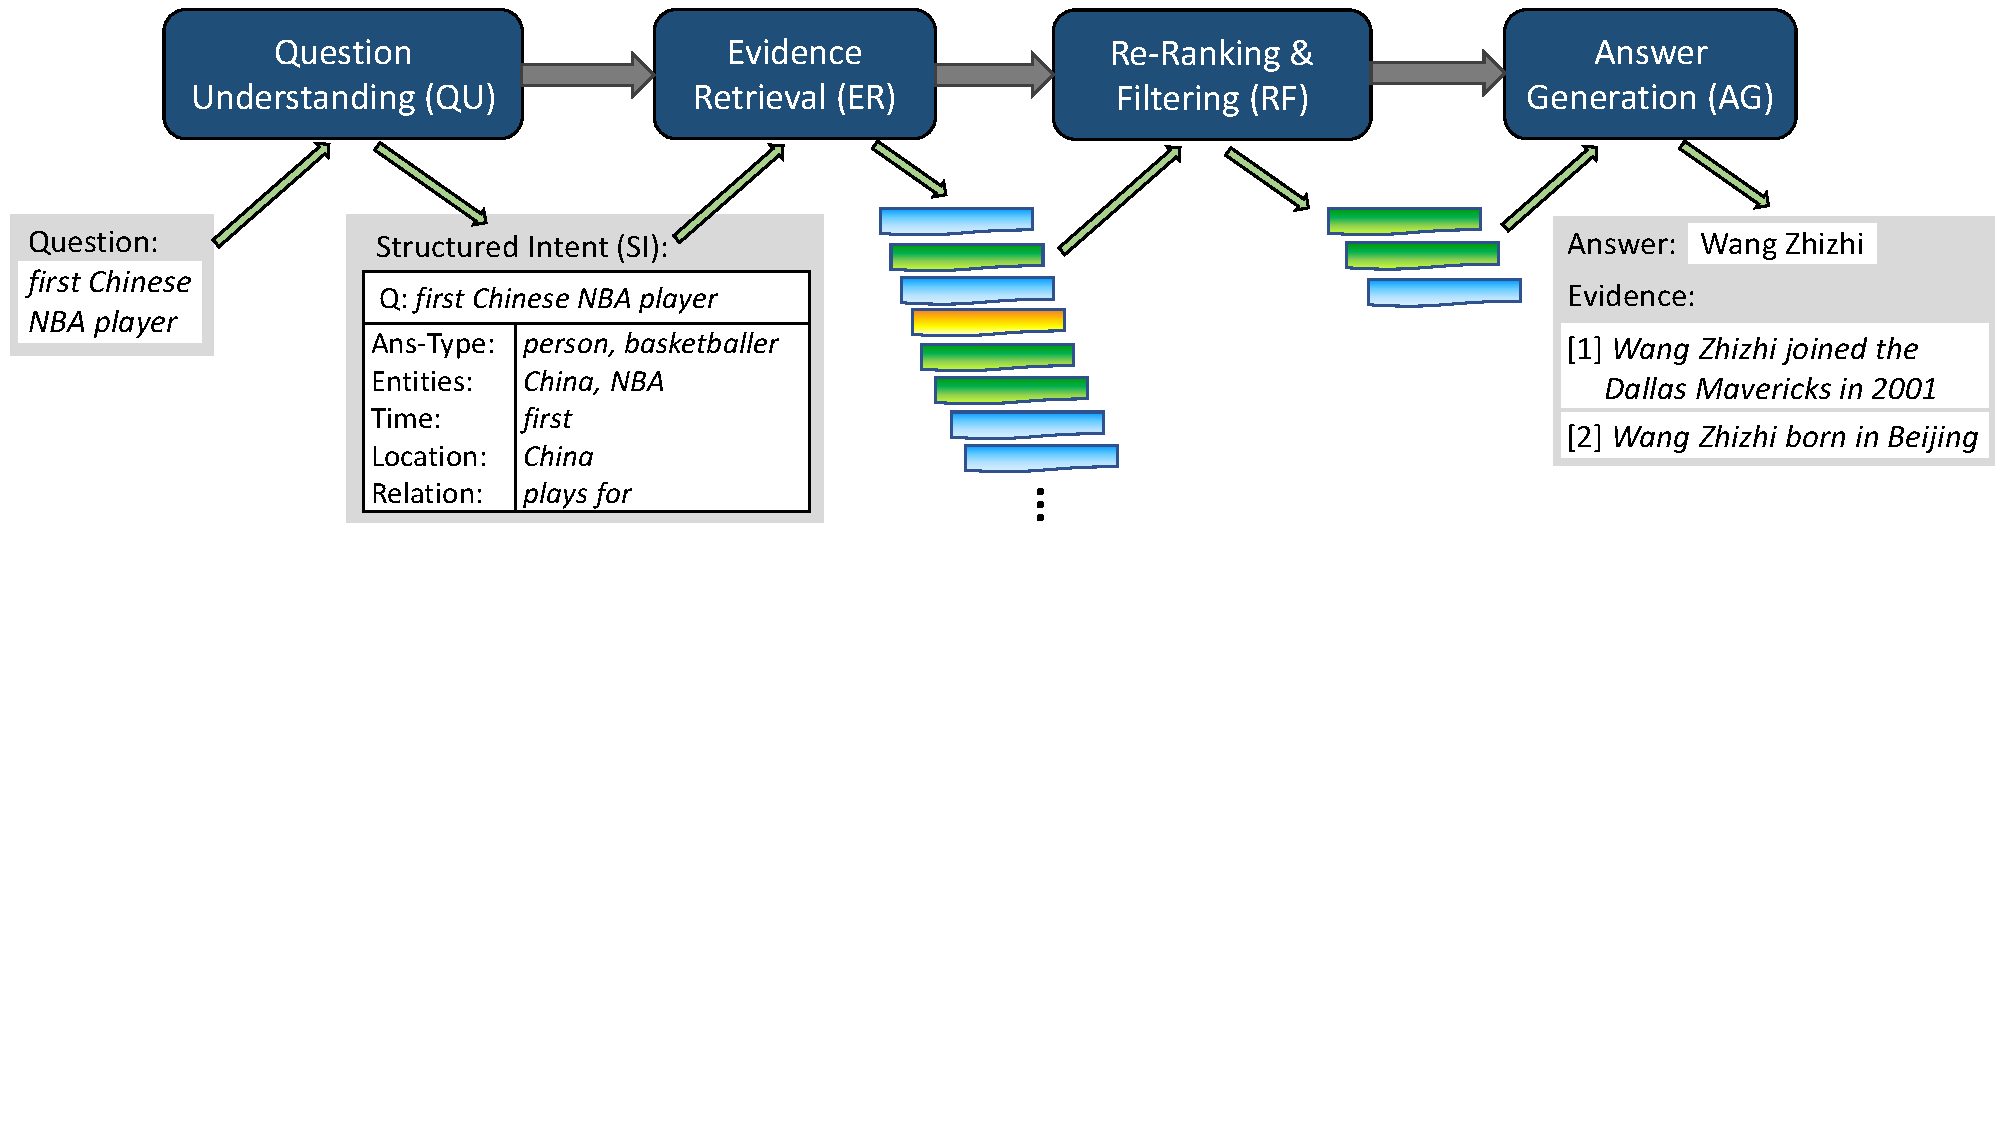
\includegraphics[width=\textwidth]{submissions/Gerhard2024/figures/compass-overview.pdf}
  \caption{Overview of the \method system.}
  \label{fig:compass-overview}
\end{figure}

% start with system overview
The \method system is a pipeline of four major stages, as illustrated in Figure \ref{fig:compass-overview}.
First, the input question is analyzed and decomposed, in order to compute a {\em structured intent (SI)} representation that will pass on to the subsequent steps, along with the original question. Second, the SI is utilized to retrieve pieces of evidence from different sources: text, KG and tables. 
Third, this pool of potentially useful evidence is filtered down, with iterative re-ranking, to arrive at a tractably small set of most promising evidence.
The final stage generates the answer from this evidence,
passing back the answer as well as evidence snippets for user-comprehensible explanation.

The second and fourth stage, Evidence Retrieval (ER) and Answer Generation (AG), are fairly standard. Such a two-phase architecture was called a retriever-reader architecture~\cite{Zhu-ODQA-survey:arxiv2021}. With a modern LLM replacing the earlier kinds of neural readers, this is the core of every RAG system~\cite{DBLP:journals/arXiv/abs-2312-10997}.

Stages 1 and 3 are unique elements of our architecture, judiciously introduced to improve both effectiveness (i.e., answer quality) and efficiency (i.e., computational cost).
Question Understanding (QU) provides the ER component with crisper and semantically refined input, and
the Re-Ranking \& Filtering (RF) stage is beneficial for
distilling the best evidence from the large pool of retrieved pieces.
The following subsections elaborate on the four stages of the pipeline, emphasizing the \method-specific steps QU and RF.



\subsection{Question Understanding (QU)}

% one par introducing the SI
To prepare the retrieval from different kinds of sources, including a KG, ad-hoc tables and text documents, it is useful to analyze and decompose the user question.
In this work, we aim to cast a question into a 
{\em structured intent (SI)} representation: essentially
a frame with faceted cues as slots, or equivalently, a concise set of key-value pairs. 
Figure \ref{fig:compass-overview} gives an idealized example for the question about the first Chinese NBA player. The facets or keys of potential interest here 
are:
\squishlist
\item {\em Ans-Type:} the expected answer type (or types when considering
different levels of semantic refinement), 
\item {\em Entities:} the salient entities in the question, and 
\item {\em Relation:} phrases that indicate which relation (between Q and A entities) the user is interested in. 
\squishend
\noindent In addition, as questions can have temporal or spatial aspects, the SI also foresees slots for:
\squishlist
\item {\em Time:} cues about answer-relevant time points or spans, including relative cues (e.g., ``before Covid'') and ordinal cues (e.g., ``first''), and
\item {\em Location:} cues about answer-relevant geo-locations.
\squishend

% discuss the spectrum of different SIs
\vspace{0.2cm}
\noindent The ideal SI for example question Q2 would look like:

\begin{quote}
{\em Ans-Type:} person, basketballer; {\em Entities:} China, NBA; {\em Time:} first;
{\em Location:} China; {\em Relation:} plays for.
\end{quote}

Note that the values for these slots can be crisp like entity names or dates, but they can also take the form of surface phrases. The SI purpose and value lie in the decomposition. In practice, many questions would only lead to a subset of faceted cues, leaving some slots empty. For the example in Figure \ref{fig:compass-overview}, an alternative SI could simply consist of

\begin{quote}
{\em Ans-Type:} person; {\em Entities:} China, NBA; {\em Time:} first.
\end{quote}

\noindent Even this simplified SI can be highly beneficial in guiding the subsequent evidence retrieval.

% sketch how an LM is trained to generate SIs 
To generate the SI from a user question, we employ a (small-scale) LM, specifically BART~\cite{DBLP:conf/acl/LewisLGGMLSZ20}, a Transformer-based auto-encoder with 140M parameters.\footnote{\url{https://huggingface.co/facebook/bart-base}}
BART is pre-trained for language representation; its power for our purpose comes from fine-tuning.
To this end, we generate (question, SI) pairs by using an instruction-trained LLM like GPT-4, with few-shot in-context learning (following our earlier work~\cite{Jia-FAITH:WWW2024}). 
Note that this is a one-time action; at inference-time we only use much smaller LMs.
The generated silver-standard pairs are then used to fine-tune BART.
In the experiments in this article, we leverage pre-existing collections of silver pairs, based on the training data of the CompMix benchmark~\cite{Christmann-CompMix:WWW2024}, 
comprising $3{,}400$ such pairs.


% outline value of SI for conversations
Although this paper focuses on single-shot questions, the \method architecture is also geared for conversational QA. In that setting, the SI can play an even bigger role, as (follow-up) questions are often formulated in a rather sloppy manner -- all but self-contained. For example, a conversation could start with a clear question {\em When did Wang Zhizhi join the NBA?}, followed a few dialog steps later, by a user utterance like {\em Which teams did he play for?} or simply {\em Which teams?}.
In such an informal conversation, the system needs to {\em contextualize} each user utterance based on the preceding turns in the dialog (e.g., inferring the relevant entities Wang Zhizhi and NBA from the conversational history).
For details on conversational QA, based on our architecture, see our earlier works~\cite{Christmann-CONVINSE:SIGIR2022,Christmann-Explaignn:SIGIR2023}.







%%%%%%%%%%%%%%%%%%%%%%%%%%%%%%%%%%%%%
\subsection{Evidence Retrieval (ER)}

The ER stage taps into a knowledge graph, a corpus of text documents, and a collection of web tables.
Specifically, for the experiments, we use the Wikidata KG,
all English Wikipedia articles, and all tables that are embedded in Wikipedia pages (incl. infoboxes, which can be seen as a special case of tables). 

% specifics: Clocq etc. - and the role of the SI
\vspace{0.2cm}
\noindent{\bf Retrieval from KG:}
To retrieve evidence from the KG, we utilize our earlier work
\clocq~\cite{Christmann-CLOCQ:WSDM2022}, which provides entity disambiguations and a relevant KG-subgraph for a given query.
Unlike most other works on QA-over-KG, \clocq fetches all KG-facts that are relevant for a given entity in a single step.
For example, when querying for
NBA players, it can traverse the KG neighborhood and pick up top teams, also considering so-called qualifier nodes in Wikidata which are often used for temporal scopes. 
As the disambiguation of entity names onto the KG can be tricky and noisy (e.g., China could be mapped to Chinese sports teams in all kinds of sports), \clocq considers several possible disambiguations~\cite{Christmann-CLOCQ:WSDM2022} (typically in the order of $10$ result entities).
The queries for \clocq are 
constructed by concatenating all slots of the question's SI.
For the example query about the first Chinese NBA player,
good result entities would be Dallas Mavericks, lists about NBA seasons, MVP awards etc., and their associated facts. These provide cues, but are likely insufficient to answer the question.


\vspace{0.2cm}
\noindent{\bf Retrieval from Text and Tables:}
The disambiguated entities returned by \clocq form anchors for tapping into text and tables.
\method first identifies 
relevant text documents and tables that refer to the anchor entities. With focus on Wikipedia, these are simply the articles for the respective entities. 
\method then constructs a keyword query that concatenates all available fields of the SI.
The query is evaluated against a linearized and verbalized representation (see below) of all sentences and all table rows in the selected documents.
This returns a set of sentences and 
and individual table rows, ranked by BM25 scores.


\vspace{0.2cm}
\noindent{\bf Evidence Verbalization:}
All results from the different data sources are uniformly treated by {\em linearizing} and {\em verbalizing} them
into token sequences. For KG results, the entity-centric triple sets are linearized via breadth-first traversal of the mini-graph starting from the entity node.
For tables, results are individual rows, which are contextualized by including labels from column headers and from the DOM-tree path of the article where the table comes from. For example, a table row about Wang Zhizhi playing for Dallas (Mavericks) in the 2000-2001 season, would be expressed as:

\vspace{0.05cm}
\hspace*{0.5cm} Wang Zhizhi / NBA Career / Season: 2000-2001, Team: Dallas, Games Played: 5 \dots
\vspace{0.05cm}

\noindent Finally, results from the text corpus are already in the form of token sequences, but we can additionally prefix these with the DOM-tree labels.
We can think of this entire pool of evidence as 
an on-the-fly corpus of potentially relevant pseudo-sentences, forming the input of the subsequent RF stage.


\vspace{0.2cm}
\noindent {\bf Result Ranking:}
Overall, the ER stage compiles a substantial set of evidence, possibly many thousands of entities, text snippets and table rows. Therefore, we practically restrict the pool to a subset of high-scoring pieces, like the top-$1000$.
For scoring, a simple BM25 model (a classical IR method) is applied. 
By default, we treat all evidence pieces uniformly with global scoring, no matter whether they come from KG, text or tables. 


\subsection{Re-Ranking and Filtering (RF)}

With a pool of top-$1000$ evidence pieces, we could invoke an LLM for answer generation. However, that would face a large fraction of noise (i.e., misleading evidence) and incur high costs of computation and energy consumption. 

For both of these reasons, we have devised light-weight techniques for iteratively reducing the top-$1000$ pieces to a small subset, say top-$30$ or top-$10$, that can be fed into an LLM at much lower cost (as LLM computations and pricing are at least linear in the number of input tokens). The difficulty is, of course, to do this without losing good evidence and reducing answer presence. Our techniques for this task are based on graph neural networks (GNNs)~\cite{Wu:IEEE2021} or cross-encoders (CEs)~\cite{Dejean:arxiv2024,Lin:MC2021}.

\myparagraph{GNN-based RF}
Given a large pool of evidence pieces from all sources, a bipartite graph is constructed:
\squishlist
\item {\em nodes} being evidence pieces or entities that occur in these pieces, and
\item {\em edges} connecting an evidence piece and an entity if the entity occurs in the evidence.
\squishend


The task for the GNN is to jointly score the evidence and the entity nodes in a multi-task learning setup. The latter are the {\em answer candidates}, and the evidence should give {\em faithful explanation} for an answer.
We build on our earlier work on explainable QA~\cite{Christmann-Explaignn:SIGIR2023}.

The node encodings are initialized with cross-encoder embeddings (see below) 
for node contents and the SI of the question. The inference iteratively adjusts the encodings based on message passing from neighboring nodes.
The GNN is trained via weak supervision from question-answer pairs:
evidence nodes are labeled as relevant if they are connected to
a gold answer.
More technical details are given in~\cite{Christmann-Explaignn:SIGIR2023}.

\method invokes the GNN in multiple rounds, iteratively reducing top-$k$ to top-$k^*$ nodes with $k^* \ll k$. In practice, we would typically consider two rounds: re-ranking top-$1000$ and pruning to top-100, and then reducing to top-30 or top-10, which are passed to the answer generation stage.
Note that this keeps the GNN at a tightly controlled size, so that its computational costs at inference-time are much smaller than those of an LLM.


\myparagraph{CE-based RF}
An alternative to the GNN inference is to employ a cross-encoder for scoring and re-ranking the evidence pieces.
These are transformers (typically with a small LM like BERT) that are fine-tuned for scoring the relatedness between a query and a document~\cite{Nogueira:arxiv2019}. In our case, the comparison is between the question SI and the evidence piece. In our experiments, we make use of two different cross-encoders, 
both trained on the MS-MARCO benchmark for passage retrieval~\cite{Bajaj:arxiv2018}, 
and fine-tuned on the respective benchmark (leveraging the same weak supervision data as for the GNNs),
the difference being in model size.\footnote{\url{https://huggingface.co/cross-encoder/ms-marco-MiniLM-L-4-v2} and\\ \url{https://huggingface.co/cross-encoder/ms-marco-MiniLM-L-6-v2}}
We use the smaller model to reduce top-$1000$ to top-100, and the larger model to go further down from top-100 to top-30.




%%%%%%%%%%%%%%%%%%%%%%%%%%%%%%%%%%%%%

\subsection{Answer Generation (AG)}

The last stage follows mainstream practice to invoke an LLM in a retrieval-augmented manner.
We call a `small-scale` LLM, specifically a fine-tuned LlaMA-3.1 model (8B-Instruct)\footnote{\url{https://huggingface.co/meta-llama/Llama-3.1-8B-Instruct}}, with a prompt \footnote{The specific prompt is \phrase{SI: \textless\texttt{concatenated SI}\textgreater \hspace{0.1cm} Evidence: \textless\texttt{evidence pieces}\textgreater}.}
consisting of:

\squishlist
\item the concatenated SI of the original question, and
\item the top-30 (or other top-$k^*$ with small $k^*$) evidence pieces.
\squishend

By the previous down-filtering of the original pool of evidence pieces, this last step has affordable cost in terms of computation time and energy consumption.

\vspace{0.2cm}
\noindent{\bf Fine-Tuning the LLM:}
We considered adding an instruction to the prompting, such as {\em ``answer this question solely based on the provided evidence snippets''}.
However, this turned out to be ineffective.
The reason why the model works well without such instructions is our task-specific fine-tuning.
We perform this by running the training data of benchmarks through the \method pipeline,
and training the AG stage with the top-30 evidence pieces as input.
Thus, the fine-tuning makes the model learn the role of evidence for RAG-based QA.

\vspace{0.2cm}
\noindent{\bf Explanations:}
The top-30 evidence pieces can be used to provide users with explanation of answers.
Optionally, these could be reduced further for comprehensibility.
Alternatively, we can fine-tune the LLM to provide both answers and concise explanations.
Since we can infer which evidences in the input mention the annotated ground-truth answers,
our method could be fine-tuned to provide such \textit{answering evidences} as well (cf.~\cite{Gao-citations:emnlp2023}).

\label{sec:exp}
\section{Experiments}


\label{setup}
\subsection{Experimental setup}


%%% BENCHMARKS
\myparagraphnospace{Benchmarks} We run experiments on three benchmarks with different characteristics of questions.

\squishlist
    \item \textbf{\compmix}.
    \compmix~\cite{Christmann-CompMix:WWW2024} is a benchmark which was specifically designed for evaluating QA systems operating over heterogeneous sources. The dataset has $9{,}410$ questions, out of which $2{,}764$ are used for testing.
    Answers are crisp entity names, dates, or other literals.
    
    \item \textbf{\crag}.
    We further evaluate on a subset of the \crag~\cite{Yang-CRAG} dataset, which was recently released as a testbed for RAG-based QA systems.
    We utilize the same pipeline and sources as outlined in Section~\ref{sec:method}, without using the web snippets or APIs provided with \crag. This way we focus on entity-centric questions that do not require access to live web data (e.g., news feeds), and disregard cases where the results would be up-to-date quantities.
    This restricts the test data to $436$ entity-centric questions, still enough for a proof of concept.
    
    \item \textbf{\timequestions}.
    To showcase the generalizability of our pipeline, we conduct experiments on~\timequestions~\cite{Jia-TimeQuestions},
    a benchmark for temporal QA. The dataset requires temporal understanding and reasoning, which are well-known limitations of
    LLMs~\cite{Dhingra-time-aware-LLM:TACL2022}. \timequestions has 16{,}181 questions (3{,}237 for testing).
\squishend

Typical examples for the questions in these three benchmarks are:

\begin{quote}
\compmix: \utterance{Which player won the most number of Man-of-the-Match titles in the FIFA world cup of 2006?}\\
 \indent \crag: \utterance{What was the worldwide box office sales for little hercules?}\\ 
  \indent \timequestions: \utterance{Which club did Cristiano Ronaldo play for before joining Real Madrid?}
\end{quote}

%%% BASELINES
\myparagraph{Baselines} As competitors or reference points to \method, we study the performance of the following methods:

\squishlist
    \item \textbf{Generative LLMs}.
    We compare \method against out-of-the-box LLMs: \textbf{\gptthree} (\texttt{text-davinci-003}), \textbf{\gptfour} (\texttt{gpt-4}) 
    and \textbf{\llama} (\texttt{meta-llama/Llama-3.1-8B-Instruct}).
    The same prompt is used for all LLMs, consistent with previous work~\cite{Christmann-CompMix:WWW2024, Zhang-Spaghetti:ACL2024}:
    \phrase{Please answer the following question by providing the crisp answer entity, date, year, or numeric number. Q: \textless\texttt{question}\textgreater}.
    

    \item \textbf{Heterogeneous QA methods}.
    \convinse~\cite{Christmann-CONVINSE:SIGIR2022}, \unikqa~\cite{Oguz-UniK-QA:NAACL2022}, \explaignn~\cite{Christmann-Explaignn:SIGIR2023}
    are QA methods designed to integrate heterogeneous sources: text, tables and KG. All of these  integrate the exact same sources as \method.

    
    \item \textbf{\textsc{State-of-the-art}}.
    For \compmix and \timequestions, we also compare against state-of-the-art methods from the literature: \spaghetti~\cite{Zhang-Spaghetti:ACL2024} and \textsc{Un-Faith}~\cite{Jia-FAITH:WWW2024}, which are among the best performing systems.
    
Results are taken from the literature whenever applicable.
On \crag, we use the models trained on \compmix for \method and heterogeneous QA baselines.
\squishend



%%% METRIC(S)
\myparagraph{Metrics}
We measure \textit{precision at 1} (\textbf{P@1}) as our main metric~\cite{RoyAnand:MC2021} on all benchmarks.
On \crag, we manually annotate answer correctness, as the ground-truth answer formats vary (e.g., entity name variants, lists, sentences).

We also compute the number of neural parameters aggregated over all sub-modules (\textbf{\#Parameters}).
Parameter counts for GPT-models are taken from~\cite{Minaee-LLM-survey}
(\gptfour might have less active parameters during inference).

For further analysis we measure \textit{answer presence} (\textbf{AP@k}),
i.e. whether the answer is present in the top-$k$ ranked evidence pieces,
and \textit{mean reciprocal rank} within the top-$k$ evidences (\textbf{MRR@k}).

%%% CONFIG
\myparagraph{Configuration}
Our implementation uses the \texttt{Llama3.1-8B-Instruct} model for the AG stage.
For the QU, ER and RF stages
we adopt code from the \explaignn project.\footnote{\url{https://explaignn.mpi-inf.mpg.de}}
For the ER stage, we use \clocq, setting its specific parameters to $k=10$ and $p=1{,}000$.

As default, we use the GNN technique for the RF stage.
For efficiency, we use light-weight models for initializing
the GNN encoders -- the same models used for the CE-based RF.\footnote{\url{https://huggingface.co/cross-encoder/ms-marco-MiniLM-L-4-v2} and\\\url{https://huggingface.co/cross-encoder/ms-marco-MiniLM-L-6-v2}}
The GNNs are trained for $5$ epochs with an epoch-wise evaluation strategy,
i.e. we choose the model with the best performance on the respective dev set.
We train the GNNs on graphs with a maximum of $100$ evidence and $400$ entity nodes (as scored by BM25).
During inference, the first GNN is applied on graphs with $1{,}000$ evidence and $4{,}000$ entity nodes, shrinking the pool of evidence pieces to the top-$100$.
The second GNN then runs on graphs with $100$ evidence and $400$ entity nodes.
The factor of 4 entities per evidence (on average) holds sufficient for the observed data,
and enables batched inference.
Other parameters are kept as is.

The AG model, based on \texttt{Llama3.1-8B-Instruct}, is 
fine-tuned
for $2$ epochs with a warm-up ratio of $0.01$ and a batch size of $8$, again with an epoch-wise evaluation strategy.
Other parameters are set to the default Hugging Face
training parameters.\footnote{\url{https://huggingface.co/docs/transformers/v4.46.2/en/main_classes/trainer\#transformers.TrainingArguments}}





\subsection{Main results}
%%% MAIN TABLE
\myparagraphnospace{\method is competitive on all benchmarks}
Main results of our experiments are shown in Table~\ref{tab:main-res}.
First of all, we note that \method achieves competitive performance across all three benchmarks.

On \compmix, baselines for heterogeneous QA and \llama perform similarly,
whereas GPT-based LLMs can answer more than $50$\% of the questions correctly.
\method exhibits substantially higher performance, on par with
the state-of-the-art method \textsc{Spaghetti}~\cite{Zhang-Spaghetti:ACL2024}
(which is based on \gptfour).

On the \crag dataset, P@1 drops for all methods except for \gptfour. 
The benchmark includes realistic questions,
which can be ambiguous/confusing (\phrase{who was the director for the report?}),
on ``exotic'' entities with answers in social media (\phrase{how many members does the teknoist have?}),
or require up-to-date information (\phrase{when did chris brown release a song or album the last time?}),
and other cases that are challenging for all methods.

Finally, \method establishes new state-of-the-art performance on the \timequestions benchmark.
Interestingly, all of the tested LLMs show greatly reduced performance on this benchmark,
which inherently requires temporal understanding and reasoning
-- a known weakness of stand-alone LLMs.


\begin{table} [h]
    \centering
    \newcolumntype{G}{>{\columncolor [gray] {0.90}}c}
    \begin{tabular}{l G G G c}
        \toprule
            \textbf{Method $\downarrow$ / Benchmark $\rightarrow$} & \textbf{\compmix}  & \textbf{\crag} & \textbf{\timequestions} & \textbf{\#Parameters} \\ 
        \midrule
            \textbf{\gptthree} 
            & $0.502$ &   $-$ & $0.224$ & $175{,}000$ M  \\
            % #params from https://arxiv.org/pdf/2402.06196

            \textbf{\gptfour}
            & $0.528$ &   $\mathbf{0.633}$ & $0.306$ & $1{,}760{,}000$ M \\
            % #params from https://arxiv.org/pdf/2402.06196

            \textbf{\llama~\cite{Touvron-LLaMA}} (8B-Instruct)
            & $0.431$ &   $0.385$ & $0.178$ & $8{,}030$ M  \\
            % #params from Huggingface (8,030,257,152)
        \midrule
            \textbf{\convinse~\cite{Christmann-CONVINSE:SIGIR2022}}
            & $0.407$  &   $0.298$ & $0.423$  & $362$ M \\
            % FiD: 222,903,936 + BART (SR-generation): 139,420,416 = 362,324,352 (python explaignn/question_understanding/structured_representation/get_num_params.py)

            \textbf{\unikqa~\cite{Oguz-UniK-QA:NAACL2022}}
            & $0.440$ &   $0.280$ & $0.424$ & $223$ M  \\
            % FiD: 222,903,936 (python explaignn/heterogeneous_answering/fid_module/FiD/get_num_params.py)
    
            \textbf{\explaignn~\cite{Christmann-Explaignn:SIGIR2023}} 
            & $0.442$ &   $0.303$ & $0.525$  & $328$ M \\
            % BART (SR-generation): 139,420,416 + 2GNNs: 94520832 + 93930240 = 327,871,488

        \midrule 
            \textbf{\textsc{State-of-the-art}}
            & $\mathbf{0.565}$ 
            & $-$
            & $0.571$  & $-$ \\

            & (\textsc{Spaghetti}~\cite{Zhang-Spaghetti:ACL2024})
            & 
            & (\textsc{Un-Faith}~\cite{Jia-FAITH:WWW2024}) &  \\

        \midrule
            \textbf{\method (ours)}
            & ${0.564}$ &   $0.362$ & $\mathbf{0.754}$  & $8{,}218$ M \\
            % BART (SR-generation): 139,420,416 + LLaMA: 8,030,257,152 + GNNs: 25,670,016 + 22,268,928 =  8,217,616,510
        \bottomrule
    \end{tabular} 
    \vspace*{-0.2cm}
    \caption{End-to-end P@1 of \method and baselines on three benchmarks. Results for \gptthree and \gptfour are taken from the literature~\cite{Christmann-CompMix:WWW2024, Jia-FAITH:WWW2024}. \gptthree is not accessible anymore, hence no results on \crag.
    }
    \label{tab:main-res}
\end{table}





%%% ANSWER SOURCES
\myparagraph{Integration of heterogeneous sources is vital}
\method integrates evidence from text, KG and tables into a unified framework.
We aim to better understand how this affects the answering performance of the method.
Table~\ref{tab:sources} shows end-to-end answering performance of \method
with different combinations of the input sources.
The results clearly indicate that all types of sources contribute, with option Text+KG+Tables performing best,
with a large margin over tapping only single source types.

\begin{table} [t] 
    \centering
    \newcolumntype{G}{>{\columncolor [gray] {0.90}}c}
    \newcolumntype{H}{>{\setbox0=\hbox\bgroup}c<{\egroup}@{}}
    	\begin{tabular}{l G G G H H H c c c} 
        \toprule
            \textbf{Benchmark $\rightarrow$}
                & \multicolumn{3}{G}{\textbf{\compmix}} 
                & \multicolumn{3}{H}{\textbf{\crag}}
                & \multicolumn{3}{c}{\textbf{\timequestions}} \\ 
        \midrule
            \textbf{Input sources $\downarrow$ / Metric $\rightarrow$}
                & \textbf{P@1} & \textbf{AP@100}  & \textbf{AP@30}
                & \textbf{P@1} & \textbf{AP@100}  & \textbf{AP@30}
                & \textbf{P@1} & \textbf{AP@100}  & \textbf{AP@30} \\
            \midrule
                \textbf{Text}           &  $0.455$  &  $0.563$  &  $0.531$ &  $?$  &  $?$  &  $?$ &  $0.539$  &  $0.515$  &  $0.487$   \\
                \textbf{KG}             &  $0.481$  &  $0.677$  &  $0.637$ &  $?$  &  $?$  &  $?$ &  $0.724$  &  $0.701$  &  $0.674$   \\
                \textbf{Tables}         &  $0.432$  &  $0.501$  &  $0.482$ &  $?$  &  $?$  &  $?$ &  $0.536$  &  $0.347$  &  $0.328$   \\
            \midrule
                \textbf{Text+KG}        &  $0.537$  &  $0.749$  &  $0.706$ &  $?$  &  $?$  &  $?$ &  $0.745$  &  $\mathbf{0.776}$  &  $0.748$   \\
                \textbf{Text+Tables}    &  $0.503$  &  $0.632$  &  $0.594$ &  $?$  &  $?$  &  $?$ &  $0.567$  &  $0.578$  &  $0.549$   \\
                \textbf{KG+Tables}      &  $0.524$  &  $0.728$  &  $0.692$ &  $?$  &  $?$  &  $?$ &  $ 0.743$  &  $0.731$  &  $0.703$   \\
            \midrule
                \textbf{Text+KG+Tables}    &  $\mathbf{0.564}$  &  $\mathbf{0.759}$  &  $\mathbf{0.724}$ &  $?$ &  $?$  &  $?$ & $\mathbf{0.754}$    & $\mathbf{0.776}$  &  $\mathbf{0.749}$   \\
            \bottomrule
    \end{tabular}
    \vspace*{-0.2cm}
    \caption{Answer presence and answering precision of \method with different combinations of input sources (on the respective test sets).}
    \label{tab:sources}
\end{table}




\subsection{Analysis}

%%% TOP-K vs. 3xTOP-(K/3)
\myparagraph{Unified retrieval enhances performance}
In the RF stage, we re-rank and filter evidence from different source types,
and feed the unified top-\textit{k}* into the AG stage.
We conduct a comparison in which we consider
the top-$10$ evidence pieces from each source type individually. This gives equal influence to KG, text and tables, whereas our default is based on global ranking.
Table~\ref{tab:unified-retrieval} shows the results for this analysis, showing our default choice performs better.
The reason is that different questions require different amounts of evidence from each of the source types.

\begin{table} [t] 
    \centering
    \newcolumntype{G}{>{\columncolor [gray] {0.90}}c}
    \newcolumntype{H}{>{\setbox0=\hbox\bgroup}c<{\egroup}@{}}
    	\begin{tabular}{l G G H H} 
        \toprule
            \textbf{Input evidences $\downarrow$ / Metric $\rightarrow$} & \textbf{P@1} & \textbf{AP@30}  & \textbf{\crag} & \textbf{\timequestions} \\ 
            \midrule
                \textbf{Top-30 Text+KG+Tables (ours)}             &  $\mathbf{0.574}$  &  $\mathbf{0.710}$  &  $-$  &  $-$   \\
                \textbf{Top-10 Text + Top-10 KG + Top-10 Tables}        &  $0.560$    &  $0.709$  &  $-$  &  $-$   \\
            \bottomrule
    \end{tabular}
    \vspace*{-0.2cm}
    \caption{Answer presence and precision
    of \method for different choices of top-30 
    (on \compmix dev set).}
    \label{tab:unified-retrieval}
\end{table}


%%% NUMBER OF EVIDENCES
\myparagraph{\method works well with small amounts of evidence}
We investigate the 
influence of 
the number of evidence pieces
fed into the AG stage, varying it from $5$ to $100$.
Results are shown in Figure~\ref{fig:res-num-evidences}.
As the curve shows, there is a sharp increase in precision as we add evidence up to 30 or 40 pieces, which is around our default of top-30. This indicates that a certain amount of evidence is needed, to overcome the inherent noise and arrive at sufficient answer presence. 
As we increase the amount of evidence further, we observe a saturation effect, and eventually a degration of performance. Too much evidence not only has diminishing returns, but can actually be confusing for the AG stage. This reconfirms our heuristic choice of top-30: enough for good answering while keeping computational costs reasonably low.


\begin{figure}[t]
    \centering
    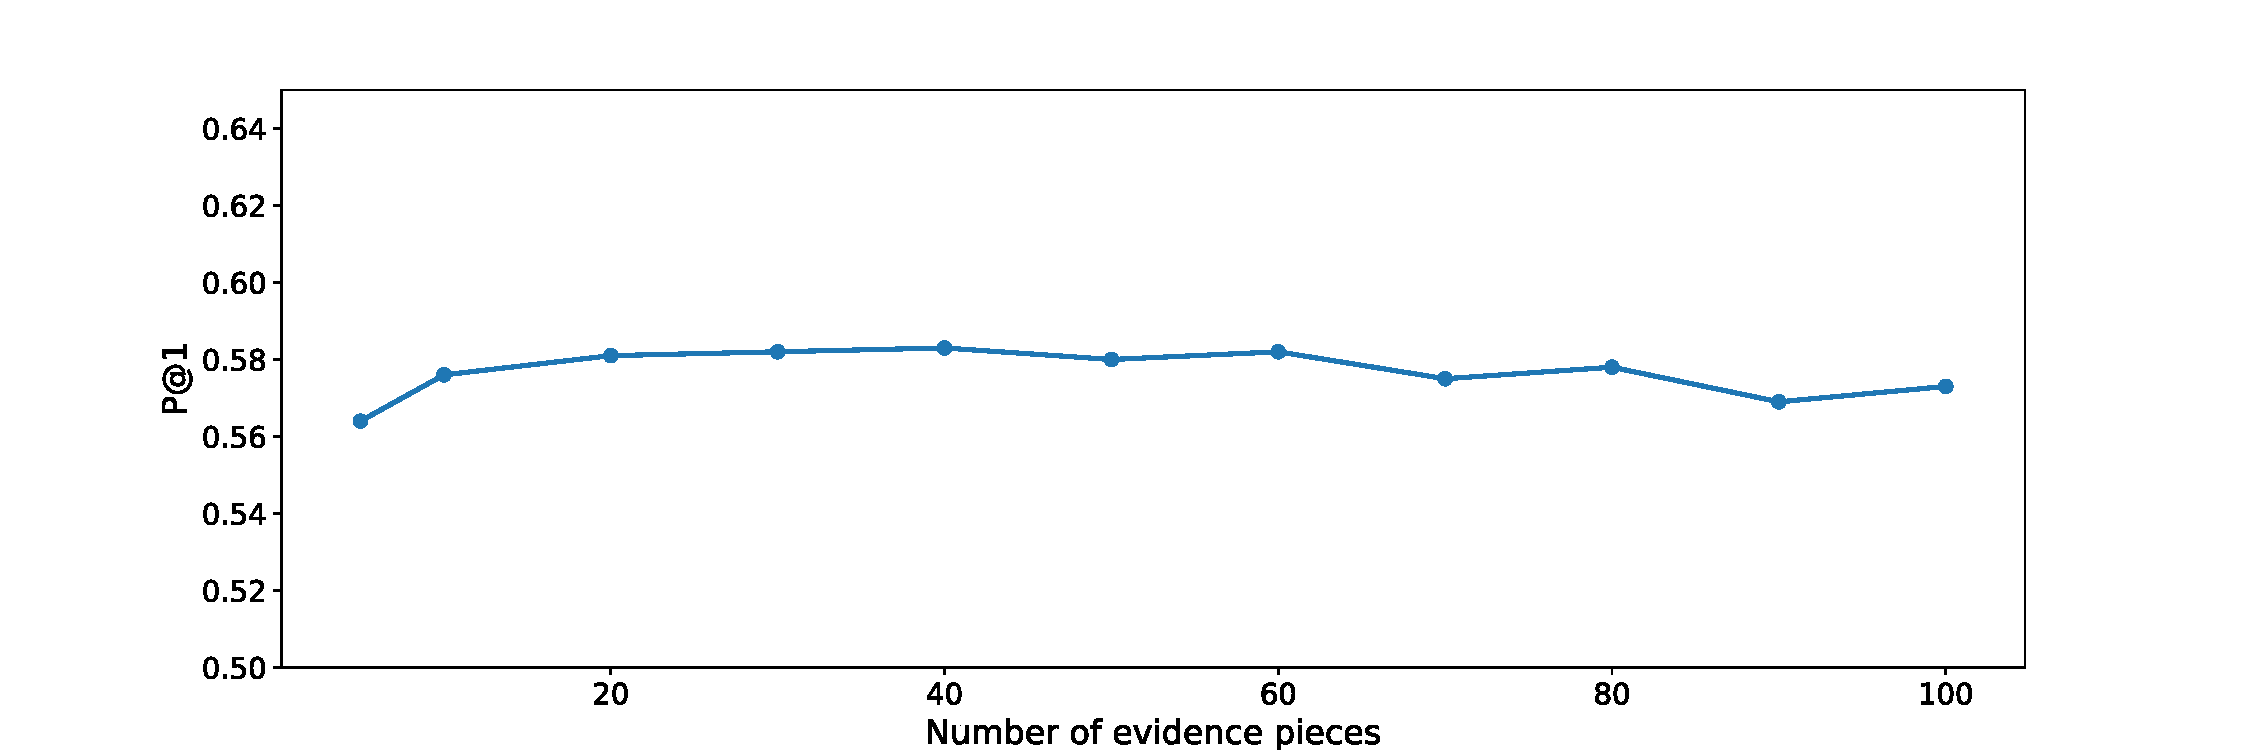
\includegraphics[width=0.8\textwidth]{submissions/Gerhard2024/figures/p_at_1-line_with_evidences.pdf}
    \vspace*{-0.2cm}
    \caption{Performance of \method on the \compmix dev set with different numbers of evidence.}
    \label{fig:res-num-evidences}
    \vspace*{-0.2cm}
\end{figure}



%%% ABLATION
\myparagraph{Ablation study on re-ranking} For more insight on the possible configurations of the RF stage, we conducted an ablation study with different options, including solely relying on the initial BM25 scoring without explicit re-ranking. The results are shown in Table \ref{tab:ablation2}. We observe that the iterative reduction in two steps is slightly better than the single-step variants (going down from top-1000 to top-30 in one RF step). Between the two options of using a GNN or a CE, the differences are negligible. A notable effect is that our RF techniques retain the answer presence at a very high level, only a bit lower than for the initial top-1000. 
The last two rows of Table \ref{tab:ablation2} demonstrate that RF is crucial: without explicit re-ranking, the technique of just picking smaller top-$k$ from the original BM25 model leads to substantial degradation in both answer presence and precision. 


\begin{table} [t] \small
    \centering
    \newcolumntype{G}{>{\columncolor [gray] {0.90}}c}
    \newcolumntype{H}{>{\setbox0=\hbox\bgroup}c<{\egroup}@{}}
    	\begin{tabular}{l G H G G G} 
        \toprule
            & \multicolumn{5}{G}{\textbf{\compmix} (dev set)} \\
        \midrule
            \textbf{RF Method $\downarrow$ / Metric $\rightarrow$} & \textbf{P@1} & \textbf{AP@1000} & \textbf{AP@100}  & \textbf{AP@30} & \textbf{MRR@100} \\ 
        \midrule
            \textbf{GNN: 1000 $\rightarrow$ 100 $\rightarrow$ 30}             &  $\mathbf{0.574}$  & $0.760$ &  $0.738$  &  $0.710$  &  $\mathbf{0.572}$  \\
            \textbf{CE: 1000 $\rightarrow$ 100 $\rightarrow$ 30}          &  $0.573$  & $0.760$  &   $\mathbf{0.740}$ &  $\mathbf{0.721}$   &  $0.553$   \\
        \midrule
            \textbf{GNN: 1000 $\rightarrow$ 30} &  $0.567$  & $?$  &   $n/a$ &  $0.710$   &  $0.567$   \\
         \textbf{CE: 1000 $\rightarrow$ 30} &  $0.570$  & $0.760$  &   $n/a$ &  $0.715$   &  $0.558$   \\
            \midrule
           \textbf{BM25: 100 (w/o GNN or CE)} &  $0.490$ & $0.760$  &  $0.652$  &  $n/a$  &  $0.259$ \\       
            \textbf{BM25: 30 (w/o GNN or CE)} &  $0.468$  & $0.760$  &  $n/a$ &  $0.534$   &  $0.259$   \\
            \bottomrule
    \end{tabular}
    \vspace*{-0.2cm}
    \caption{Ablation study for different RF strategies of \method on the \compmix dev set. The answer presence in the RF input with top-$1000$ evidence pieces is $0.760$.}
    \label{tab:ablation2}
\end{table}



\myparagraph{Quality of SI}
To assess the quality and robustness of the Structured Intents, we
inspected a sample of questions and their SIs.
Table~\ref{tab:question-SI-examples} gives three anecdotic examples.
We show SIs generated by \method, which makes use of the pre-existing collection from the \compmix benchmark for training.
This training data was obtained via different heuristics, 
which can be a limiting factor when user intents become more complex.

Therefore, we also looked at SIs derived via in-context learning (ICL) using \gptfour with $5$ handcrafted examples.
As shown in our earlier work on temporal QA~\cite{Jia-FAITH:WWW2024},
such data can be used for training smaller models (e.g., BART),
which can greatly boost the completeness and overall quality of the generated SIs.

From the sampled set, we observed that the ICL-based SIs are more
complete with all slots filled, whereas the BART-based SIs focused more
on the main slots Answer-type, Entities and Relation.
However, both approaches achieve very high quality in filling the slots,
capturing the user's information need very well.

Interestingly, when questions get complicated, with nested phrases, 
the ICL-based variant succeeds in decomposing the questions, based on only $5$ ICL examples.
For example, for the question {\em ``which German state had the most Corona-related death cases in the first year after the outbreak?''}
the Time slot becomes {\em ``first year after Corona outbreak''},
which can be resolved to identify the temporal scope.
In general, we believe that such question decomposition, beyond simple temporal constraints,
would be an interesting theme for future work.

\begin{table} [t] 
    \centering
    \small
    \newcolumntype{G}{>{\columncolor [gray] {0.90}}c}
    \newcolumntype{H}{>{\setbox0=\hbox\bgroup}c<{\egroup}@{}}
    \resizebox*{\textwidth}{!}{
        \begin{tabular}{p{6cm}|p{6cm}|p{6cm}} 
        \toprule
            \textbf{Question} & \textbf{Current SI by \method} & \textbf{SI via ICL} \\
        \midrule
        \textit{what was disneys first color movie?}
            & Ans-Type: \textit{animated feature film} & Ans-Type: \textit{film, animated film} \\
            & Entities: \textit{disneys} & Entities: \textit{Disney} \\
            & Relation: \textit{was first color movie} & Relation: \textit{first color movie} \\
            &  & Time: \textit{first} \\
        \midrule
        \textit{at the oscars, who won best actor in 2018?}
            & Ans-Type: \textit{human} & Ans-Type: \textit{person, actor} \\
            & Entities: \textit{at the oscars} & Entities: \textit{Oscars, 2018} \\
            & Relation: \textit{who won best actor in 2018} & Relation: \textit{won best actor} \\
            &  & Time: \textit{2018} \\
        \midrule
        \textit{which German state had the most Corona-} & Ans-Type: \textit{state} & Ans-Type: \textit{location, state} \\
        \textit{related death cases in the first year after} & Entities: \textit{Germany, Corona} & Entities: \textit{Germany, Corona-related deaths} \\
        \textit{the outbreak?} & Relation: \textit{which state had the most related} & Relation: \textit{highest count of death cases} \\
        & \textit{death cases in the first year after the out-}  & Location: \textit{Germany} \\
            & \textit{break}  & Time: \textit{first year after Corona outbreak} \\
        \bottomrule
    \end{tabular}
    }
    \vspace*{-0.2cm}
    \caption{Examples for pairs of question and generated SI.}
    \label{tab:question-SI-examples}
\end{table}




%%% REFRAIN FROM ANSWER
\myparagraph{Refraining from answering}
%%% Searched for: "generated_answer I" (with I being the full word, not partial) in the generated answers of LLaMA
%%% yields 245 results out of 2764 questions on CompMix
%%% yields 1270 results out of 3237 questions on TimeQuestions
We can train our model to refrain from answering in scenarios
where the provided evidence does not contain an answer to the question.
Specifically, during training, when the answer is not present in the evidence,
we change the target answer to {\em unknown}. This variant is referred to as \method {\em (faithful)}.

We measure the ratio of questions for which {\em unknown} is provided as answer,
and the P@1 restricted to questions that are answered.
The accuracy of refraining from answering is measured as well,
based on whether the answer is present in the evidence or not.
We conduct this experiment on \compmix and \timequestions,
for which we can compute answer presence exactly.
We also compute results for \llama, which is already instructed 
with the option to answer ``don't know''.
Table~\ref{tab:refrain-from-answer} shows the results.
For \compmix, we observe that \method has high accuracy on refraining when appropriate,
whereas \llama tends to be overconfident with a very small rate of {\em unknowns}, leading to incorrect answers.

\begin{table} [t] \small
    \centering
    \newcolumntype{G}{>{\columncolor [gray] {0.90}}c}
    \newcolumntype{H}{>{\setbox0=\hbox\bgroup}c<{\egroup}@{}}
    	\begin{tabular}{l G G G G c c c c} 
        \toprule
            & \multicolumn{4}{G}{\textbf{\compmix}} & \multicolumn{4}{c}{\textbf{\timequestions}} \\
            \midrule
            \textbf{Metric $\rightarrow$} & \textbf{P@1}  & \textbf{P@1} & \textbf{Refrain} & \textbf{Refrain} & \textbf{P@1}  & \textbf{P@1} & \textbf{Refrain} & \textbf{Refrain} \\ 
            \textbf{Method $\downarrow$} &                 & \textbf{(answered)} & \textbf{rate} & \textbf{accuracy} &                 & \textbf{(answered)} & \textbf{rate} & \textbf{accuracy} \\ 
            \midrule
                \textbf{\llama}             &  $0.431$  &  $0.471$  &  $0.089$  &  $n/a$  &  $0.177$  &  $0.276$  &  $0.392$  &  $n/a$  \\
                \textbf{\method (faithful)}           &  $0.497$  &  $0.713$  &  $0.303$  &  $0.838$ &  $0.597$  &  $0.804$  &  $0.257$  &  $0.864$  \\
            \bottomrule
    \end{tabular}
    \vspace*{-0.2cm}
    \caption{
        Performance of \method with option to refrain from answering (``don't know'').
    }
    \label{tab:refrain-from-answer}
\end{table}

\label{sec:disc}
\section{Insights, Limitations, and Challenges}


\noindent{\bf Benchmark Performance.} Our method, RAG-based \method with an 8B LLaMA model, outperforms much larger LLMs like \gptfour on two of the three benchmarks, with a very large margin for temporal questions. Obviously, pre-trained LLMs have only limited sense of properly positioning ``remembered’’ facts on the timeline even with training data that exceeds ours by several orders of magnitude. This confirms our intuition that LLMs alone are not good at ``recalling’’  higher-arity relations that require combining distant pieces of evidence. This is a sweet spot for RAG. Only for 
the \crag benchmark, \method is substantially inferior to a full-blown LLM. This is likely due to the nature of the questions: not necessarily the complexity of the information needs, but the need for more web sources (beyond what our experiments tap into).

\vspace{0.2cm}
\noindent{\bf Cost/Performance Ratio.} The most important take-away from our experiments is that \method achieves its competitive performance at a much lower cost than the full LLMs. Assuming that the consumed GFlops are proportional to the number of model parameters, \method achieves a cost reduction by a factor of 200x for \gptthree and 2000x for \gptfour. This does not only mean less computation, but also a massively lower electricity bill and climate impact.  

\vspace{0.2cm}
\noindent{\bf Role of Question Understanding.} We did not systematically investigate the influence of the Structured Intent in the \method pipeline. However, the comparison to the big GPT models reflects the role of the SI, as we prompt the GPT models in their natural mode with the original questions. The linearized sequence of available SI slots does not always have major advantages, but there are enough cases where specific facets provide crucial cues. This holds especially for the Entities slot, as this drives the gathering of evidence in the ER stage (cf.~\cite{Christmann-CONVINSE:SIGIR2022}, and for the Time slot, as these cues are often decisive for temporal questions (cf.~\cite{Jia-FAITH:WWW2024}).

\vspace{0.2cm}
\noindent{\bf Role of Re-Ranking.} As our ablation studies show, merely using top-$k$ evidence from an initial BM25-style ranking does not provide good performance. Also, there seems to be sweet spot in the choice of $k$: we need enough evidence for connecting the dots if the question requires multiple pieces of information, or for corroborating candidates if the question finds many useful but noisy pieces. In the experiments, $k=30$ turns out to be good choice; much lower $k$ results in insufficient evidence, and much larger $k$ leads to saturation and ultimately degrading performance. Our argument for iteratively shrinking the candidate set in multiple rounds of re-ranking is substantiated in our experiments, but the gain of doing this, compared to GNN- or CE-based re-ranking from 1000 to 30, is not big. More research is called to better understand the role of ranking in RAG. 

\vspace{0.2cm}
\noindent{\bf Limitations of Evidence Retrieval.}
For ER, we adopted more or less standard techniques. The results showed very good answer presence, in the order of 75\% in the top-100 or even top-30. An important case where this is insufficient are questions that require aggregating information over a large number of evidence pieces. An example is asking for the life-time total of 3-point scores of the basketball player Dirk Nowitzki.
This requires collecting a set of per-season tables with NBA player statistics, but also other web sources with numbers for his career before he joined the NBA (including his youth teams).
Of course, there are sometimes shortcuts like a Wikipedia article or biography mentioning the total number, but this cannot be universally assumed. The bottom line is that ER should be reconsidered as well, striving to improve the recall dimension.

\vspace{0.2cm}
\noindent{\bf Limitations of Answer Generation.}
For AG, we simply rely on a LLM,
using it as an extractor (``reader'') from the given evidence. Despite the wide belief that LLMs can perform deep
reasoning over many pieces of evidence, our experience is that the extraction works only well – robustly and faithfully – for relatively simple questions with a few multi-hop joins or simple aggregation over a few pieces. However, complicated questions such as asking for the top-100 NBA players with the largest number of life-time 3-point scores (again including their pre-NBA careers) are currently out of scope and will likely remain so for quite some time. This offers many opportunities for pushing the envelope further.

\vspace{0.2cm}
\noindent{\bf Trust in Data Sources.}
In our experiments, we considered all heterogeneous sources as trustworthy and unbiased. With focus on Wikidata and Wikipedia, this assumption has been well justified. In the wild, however, input data for RAG-based systems likely exhibit a wide spectrum of quality issues, in terms of stale information, biased positions, or simply false statements. Identifying trustworthy and up-to-date evidence and dealing with conflicting data, has been explored in other contexts (e.g., for KG curation~\cite{Dong-Trust:PVLDB2015}), but remains a major challenge for RAG-based QA.


\vspace{0.2cm}
\noindent{\bf Open Challenges and Future Work.} The best-performing methods in our experiment, mostly \method, reach P@1 values of 56\% for \compmix and 75\% for \timequestions. 
For the latter, the answer presence in the top-100 is only slightly higher; so the AG stage hardly misses anything.
However, for \compmix, the answer presence is 75\% -- much higher than what our system can actually answer. Obviously, closing this gap is a major direction to pursue, with focus on the RF and AG stages. However, missing one fourth of the answers completely in the top-100 pool, is a big problem as well. This requires improving recall at the ER stage, possibly with better guidance by the QU, which in turn needs more sources beyond the scope of our experiments (currently limited to Wikidata and Wikipedia). 

In general, we need to think beyond this kind of ``benchmark mindset’’. Even if we reached 80\% or 90\% precision and recall, we would still have a substantial fraction of questions that are answered incorrectly
or not at all. 
The remaining errors may not be a problem for chatbots, but they would be a showstopper for the deployment of mission-critical applications in business or science. We believe that this big gap is a shortcoming of {\em all methods}, not an issue that comes from the data alone. For trivia-style QA, as looked at in this paper, a smart human in ``open book’’ mode and no time limitation should be able to properly answer practically all questions, just by reading pieces of web contents and putting things together. Neither LLMs nor state-of-the-art RAG are the final solution; substantial research and creative ideas are needed to further advance QA.


\clearpage
\newpage

\newcommand{\bibauthors}[1]{{#1}}
\newcommand{\bibtitle}[1]{\emph{#1}}
\newcommand{\bibconf}[1]{{#1}}

\begin{thebibliography}{10}

\bibitem{Bajaj:arxiv2018}
\bibauthors{Payal Bajaj, Daniel Campos, Nick Craswell, Li Deng, Jianfeng Gao, Xiaodong Liu, Rangan Majumder, Andrew McNamara, Bhaskar Mitra, Tri Nguyen, Mir Rosenberg, Xia Song, Alina Stoica, Saurabh Tiwary, Tong Wang.}
\bibtitle{MS MARCO: A Human Generated MAchine Reading COmprehension Dataset.}
In \bibconf{arXiv 2018}.

\bibitem{DBLP:conf/acl/ChenFWB17}
\bibauthors{Danqi Chen, Adam Fisch, Jason Weston and Antoine Bordes.}
\bibtitle{Reading Wikipedia to Answer Open-Domain Questions.}
In \bibconf{ACL 2017}.

\bibitem{Christmann-CONVINSE:SIGIR2022}
\bibauthors{Philipp Christmann, Rishiraj Saha Roy, Gerhard Weikum.}
\bibtitle{Conversational Question Answering on Heterogeneous Sources.}
In \bibconf{SIGIR 2022}.

\bibitem{Christmann-CLOCQ:WSDM2022}
\bibauthors{Philipp Christmann, Rishiraj Saha Roy, Gerhard Weikum.}
\bibtitle{Beyond NED: Fast and Effective Search Space Reduction for Complex Question Answering over Knowledge Bases.}
In \bibconf{WSDM 2022}.

\bibitem{Christmann-Explaignn:SIGIR2023}
\bibauthors{Philipp Christmann, Rishiraj Saha Roy, Gerhard Weikum.}
\bibtitle{Explainable Conversational Question Answering over Heterogeneous Sources via Iterative Graph Neural Networks.}
In \bibconf{SIGIR 2023}.

\bibitem{Christmann-CompMix:WWW2024}
\bibauthors{Philipp Christmann, Rishiraj Saha Roy, Gerhard Weikum.}
\bibtitle{CompMix: A Benchmark for Heterogeneous Question Answering.}
In \bibconf{WWW 2024}.

\bibitem{Dejean:arxiv2024}
\bibauthors{Herve Dejean, Stephane Clinchant, Thibault Formal.}
\bibtitle{A Thorough Comparison of Cross-Encoders and LLMs for Reranking SPLADE.}
In \bibconf{arXiv 2024}.

\bibitem{Dhingra-time-aware-LLM:TACL2022}
\bibauthors{Bhuwan Dhingra, Jeremy R Cole, Julian Martin Eisenschlos, Daniel Gillick, Jacob Eisenstein, and William W Cohen.}
\bibtitle{Time-Aware Language Models as Temporal Knowledge Bases.}
In \bibconf{TACL 2022}.

\bibitem{Dong-Trust:PVLDB2015}
\bibauthors{Xin Luna Dong, Evgeniy Gabrilovich, Kevin Murphy, Van Dang, Wilko Horn, Camillo Lugaresi, Shaohua Sun, Wei Zhang.}
\bibtitle{Knowledge-Based Trust: Estimating the Trustworthiness of Web Sources.}
In \bibconf{PVLDB 2015}.

\bibitem{DBLP:journals/arXiv/abs-2312-10997}
\bibauthors{Yunfan Gao, Yun Xiong, Xinyu Gao, Kangxiang Jia, Jinliu Pan, Yuxi Bi, Yi Dai, Jiawei Sun, Qianyu Guo, Meng Wang, Haofen Wang.}
\bibtitle{Retrieval-Augmented Generation for Large Language Models: A Survey.}
In \bibconf{arXiv 2023}.

\bibitem{Gao-citations:emnlp2023}
\bibauthors{Tianyu Gao, Howard Yen, Jiatong Yu, Danqi Chen.}
\bibtitle{Enabling Large Language Models to Generate Text with Citations.}
In \bibconf{EMNLP 2023}.

\bibitem{Guu-REALM:ICML2020}
\bibauthors{Kelvin Guu, Kenton Lee, Zora Tung, Panupong Pasupat, Ming-Wei Chang.}
\bibtitle{Retrieval Augmented Language Model Pre-Training.}
In \bibconf{ICML 2020}.

\bibitem{DBLP:conf/eacl/IzacardG21}
\bibauthors{Gautier Izacard, Edouard Grave.}
\bibtitle{Leveraging Passage Retrieval with Generative Models for Open Domain Question Answering.}
In \bibconf{EACL 2021}.

\bibitem{Jia-TimeQuestions}
\bibauthors{Zhen Jia, Soumajit Pramanik, Rishiraj Saha Roy, and Gerhard Weikum.}
\bibtitle{Complex Temporal Question Answering on Knowledge Graphs.}
In \bibconf{CIKM 2021}.

\bibitem{Jia-FAITH:WWW2024}
\bibauthors{Zhen Jia, Philipp Christmann, Gerhard Weikum.}
\bibtitle{Faithful Temporal Question Answering over Heterogeneous Sources.}
In \bibconf{WWW 2024}.

\bibitem{DBLP:journals/arXiv/abs-2305-06984}
\bibauthors{Ehsan Kamalloo, Nouha Dziri, Charles L. A. Clarke, Davood Rafiei.}
\bibtitle{Evaluating Open-Domain Question Answering in the Era of Large Language Models.}
In \bibconf{arXiv 2023}.

\bibitem{Kandpal:ICML2023}
\bibauthors{Nikhil Kandpal, Haikang Deng, Adam Roberts, Eric Wallace, Colin Raffel.}
\bibtitle{Large Language Models Struggle to Learn Long-Tail Knowledge.}
In \bibconf{ICML 2023}.

\bibitem{DBLP:conf/emnlp/KarpukhinOMLWEC20}
\bibauthors{Vladimir Karpukhin, Barlas Oguz, Sewon Min, Patrick S. H. Lewis, Ledell Wu, Sergey Edunov, Danqi Chen, Wen-tau Yih.}
\bibtitle{Dense Passage Retrieval for Open-Domain Question Answering.}
In \bibconf{EMNLP 2020}.

\bibitem{Lee-MATTER:ACL2024}
\bibauthors{Dongkyu Lee, Chandana Satya Prakash, Jack FitzGerald, Jens Lehmann.}
\bibtitle{MATTER: Memory-Augmented Transformer Using Heterogeneous Knowledge Sources.}
In \bibconf{ACL 2024}.

\bibitem{DBLP:conf/acl/LewisLGGMLSZ20}
\bibauthors{Mike Lewis, Yinhan Liu, Naman Goyal, Marjan Ghazvininejad, Abdelrahman Mohamed, Omer Levy, Veselin Stoyanov, Luke Zettlemoyer.}
\bibtitle{BART: Denoising Sequence-to-Sequence Pre-training for Natural Language Generation, Translation, and Comprehension.}
In \bibconf{ACL 2020}.

\bibitem{DBLP:conf/nips/LewisPPPKGKLYR020}
\bibauthors{Patrick S. H. Lewis, Ethan Perez, Aleksandra Piktus, Fabio Petroni, Vladimir Karpukhin, Naman Goyal, Heinrich Küttler, Mike Lewis, Wen-tau Yih, Tim Rocktäschel, Sebastian Riedel, Douwe Kiela.}
\bibtitle{Retrieval-Augmented Generation for Knowledge-Intensive NLP Tasks.}
In \bibconf{NeurIPS 2020}.

\bibitem{Lin:MC2021}
\bibauthors{Jimmy Lin, Rodrigo Frassetto Nogueira, Andrew Yates.}
\bibtitle{Pretrained Transformers for Text Ranking: BERT and Beyond.}
In \bibconf{Morgan \& Claypool Publishers 2021}.

\bibitem{Liu-SUQL:NAACL2024}
\bibauthors{Shicheng Liu, Jialiang Xu, Wesley Tjangnaka, Sina J. Semnani, Chen Jie Yu, Monica Lam.}
\bibtitle{SUQL: Conversational Search over Structured and Unstructured Data with Large Language Models.}
In \bibconf{NAACL-HLT 2024}.

\bibitem{Mavi:FnT2024}
\bibauthors{Vaibhav Mavi, Anubhav Jangra, Adam Jatowt.}
\bibtitle{Multi-hop Question Answering.}
In \bibconf{Foundations and Trends in Information Retrieval 2024}.

\bibitem{Minaee-LLM-survey}
\bibauthors{Shervin Minaee, Tomas Mikolov, Narjes Nikzad, Meysam Chenaghlu, Richard}
\bibtitle{Socher, Xavier Amatriain, and Jianfeng Gao.}
Large Language Models: A Survey.
In \bibconf{arXiv 2024}.

\bibitem{Nogueira:arxiv2019}
\bibauthors{Rodrigo Frassetto Nogueira, Kyunghyun Cho.}
\bibtitle{Passage Re-ranking with BERT.}
In \bibconf{arXiv 2019}.

\bibitem{Oguz-UniK-QA:NAACL2022}
\bibauthors{Barlas Oguz, Xilun Chen, Vladimir Karpukhin, Stan Peshterliev, Dmytro Okhonko, Michael Sejr Schlichtkrull, Sonal Gupta, Yashar Mehdad, Scott Yih.}
\bibtitle{UniK-QA: Unified Representations of Structured and Unstructured Knowledge for Open-Domain Question Answering.}
In \bibconf{NAACL-HLT 2022}.

\bibitem{RogersGA:CS2023}
\bibauthors{Anna Rogers, Matt Gardner, Isabelle Augenstein.}
\bibtitle{QA Dataset Explosion: A Taxonomy of NLP Resources for Question Answering and Reading Comprehension.}
In \bibconf{ACM Computing Surveys 2023}.

\bibitem{RoyAnand:MC2021}
\bibauthors{Rishiraj Saha Roy, Avishek Anand.}
\bibtitle{Question Answering for the Curated Web: Tasks and Methods in QA over Knowledge Bases and Text Collections.}
In \bibconf{Synthesis Lectures on Information Concepts, Retrieval, and Services, Morgan \& Claypool Publishers 2021}.

\bibitem{Pramanik-Uniqorn:JWS2024}
\bibauthors{Soumajit Pramanik, Jesujoba Alabi, Rishiraj Saha Roy, Gerhard Weikum.}
\bibtitle{UNIQORN: Unified Question Answering over RDF Knowledge Graphs and Natural Language Text.}
In \bibconf{Journal of Web Semantics 2024}.

\bibitem{Sun-PullNet:EMNLP2019}
\bibauthors{Haitian Sun, Tania Bedrax-Weiss, William W. Cohen.}
\bibtitle{PullNet: Open Domain Question Answering with Iterative Retrieval on Knowledge Bases and Text.}
In \bibconf{EMNLP/IJCNLP 2019}.

\bibitem{Sun:NAACL2024}
\bibauthors{Kai Sun, Yifan Ethan Xu, Hanwen Zha, Yue Liu, Xin Luna Dong.}
\bibtitle{Head-to-Tail: How Knowledgeable are Large Language Models (LLMs)? A.K.A. Will LLMs Replace Knowledge Graphs?}
In \bibconf{NAACL-HLT 2024}.

\bibitem{Touvron-LLaMA}
\bibauthors{Hugo Touvron, Thibaut Lavril, Gautier Izacard, Xavier Martinet, Marie-Anne Lachaux, Timothée Lacroix, Baptiste Rozière, Naman Goyal, Eric Hambro, Faisal Azhar, Aurelien Rodriguez, Armand Joulin, Edouard Grave, Guillaume Lample.}
\bibtitle{Llama: Open and efficient foundation language models.}
In \bibconf{arXiv 2023}.

\bibitem{Wu-STARK:arxiv2024}
\bibauthors{Shirley Wu, Shiyu Zhao, Michihiro Yasunaga, Kexin Huang, Kaidi Cao, Qian Huang, Vassilis N. Ioannidis, Karthik Subbian, James Zou, Jure Leskovec.}
\bibtitle{STaRK: Benchmarking LLM Retrieval on Textual and Relational Knowledge Bases.}
In \bibconf{arXiv 2024}.

\bibitem{Wu:IEEE2021}
\bibauthors{Zonghan Wu, Shirui Pan, Fengwen Chen, Guodong Long, Chengqi Zhang, Philip S. Yu.}
\bibtitle{A Comprehensive Survey on Graph Neural Networks.}
In \bibconf{IEEE Transactions on Neural Networks and Learning Systems 2021}.

\bibitem{Yang-CRAG}
\bibauthors{Xiao Yang, Kai Sun, Hao Xin, Yushi Sun, Nikita Bhalla, Xiangsen Chen, Sajal Choudhary, Rongze D. Gui, Ziran W. Jiang, Ziyu Jiang, Lingkun Kong, Brian Moran, Jiaqi Wang, Yifan Ethan Xu, An Yan, Chenyu Yang, Eting Yuan, Hanwen Zha, Nan Tang, Lei Chen, Nicolas Scheffer, Yue Liu, Nirav Shah, Rakesh Wanga, Anuj Kumar, Wen-tau Yih, Xin Luna Dong.}
\bibtitle{CRAG -- Comprehensive RAG Benchmark.}
In \bibconf{arXiv 2024}.

\bibitem{Yasunaga:NAACL2021}
\bibauthors{Michihiro Yasunaga, Hongyu Ren, Antoine Bosselut, Percy Liang, Jure Leskovec.}
\bibtitle{QA-GNN: Reasoning with Language Models and Knowledge Graphs for Question Answering.}
In \bibconf{NAACL-HLT 2021}.

\bibitem{Zhang-Spaghetti:ACL2024}
\bibauthors{Heidi C. Zhang, Sina J. Semnani, Farhad Ghassemi, Jialiang Xu, Shicheng Liu, Monica S. Lam.}
\bibtitle{SPAGHETTI: Open-Domain Question Answering from Heterogeneous Data Sources with Retrieval and Semantic Parsing.}
In \bibconf{ACL 2024}.

\bibitem{Zhang:NAACL2024}
\bibauthors{Jiahao Zhang, Haiyang Zhang, Dongmei Zhang, Yong Liu, Shen Huang.}
\bibtitle{End-to-End Beam Retrieval for Multi-Hop Question Answering.}
In \bibconf{NAACL-HLT 2024}.

\bibitem{Zhao-LLMsurvey}
\bibauthors{Wayne Xin Zhao, Kun Zhou, Junyi Li, Tianyi Tang, Xiaolei Wang, Yupeng Hou, Yingqian Min, Beichen Zhang, Junjie Zhang, Zican Dong, Yifan Du, Chen Yang, Yushuo Chen, Zhipeng Chen, Jinhao Jiang, Ruiyang Ren, Yifan Li, Xinyu Tang, Zikang Liu, Peiyu Liu, Jian-Yun Nie, Ji-Rong Wen.}
\bibtitle{A Survey of Large Language Models.}
In \bibconf{arXiv 2023}.

\bibitem{Zhao:arxiv2024}
\bibauthors{Penghao Zhao, Hailin Zhang, Qinhan Yu, Zhengren Wang, Yunteng Geng, Fangcheng Fu, Ling Yang, Wentao Zhang, Bin Cui.}
\bibtitle{Retrieval-Augmented Generation for AI-Generated Content: A Survey.}
In \bibconf{arXiv 2024}.

\bibitem{Zhu-ODQA-survey:arxiv2021}
\bibauthors{Fengbin Zhu, Wenqiang Lei, Chao Wang, Jianming Zheng, Soujanya Poria, Tat-Seng Chua.}
\bibtitle{Retrieving and Reading: A Comprehensive Survey on Open-domain Question Answering.}
In \bibconf{arXiv 2021}.

\end{thebibliography}


\end{document}
 
\end{article}
\begin{article}
{Does Differential Privacy Impact Bias in Pretrained Language Models?}
{Md. Khairul Islam, Andrew Wang, Tianhao Wang, Yangfeng Ji, Judy Fox, Jieyu Zhao}
\documentclass{article}

\usepackage{deauthor}

\usepackage{latexsym}
\usepackage{graphicx}
\graphicspath{{./images/}}
\usepackage{booktabs} % for formal tables
\usepackage{color}  % for coloring text
\usepackage{amsmath}  % for aligning equations
\usepackage{subcaption}
\usepackage{caption}
\usepackage{tikz}
\usepackage{colortbl} % for color in tables
\usepackage{framed}
\usepackage{multirow}
\usepackage{multicol}
\usepackage{hyperref}
\usepackage{url}
\usepackage{balance}
\usepackage{verbatim}
\usepackage{cancel}
\usepackage{xspace} % for correcting space after macro commands
\usepackage{algorithm2e}
\usepackage{bbold} % for writing mathbb{1}
\usepackage{balance}
\usepackage{stmaryrd}
\usepackage{enumitem}
\usepackage{array} % package for hiding a column
\usepackage{bold-extra} % to enable textbf with textsc

% used for making text readable in document and .tex
% \setlength{\parindent}{0pt}

\newcommand{\struct}[1]{\texttt{\small #1}}
\newcommand{\utterance}[1]{\textit{#1}}
\newcommand{\phrase}[1]{\textit{``#1''}}

% \newcommand {\g}[1]{\textcolor[gray]{0.6}{#1}}

\newcommand{\drop}{\dag\xspace}

\newenvironment{Snugshade}[1][236,236,236]{
    \setlength{\itemsep}{0pt}
     \setlength{\parsep}{0pt}
     \setlength{\topsep}{0pt}
     \setlength{\partopsep}{0pt}
     \setlength{\leftmargin}{1.5em}
     \setlength{\labelwidth}{0em}
     \setlength{\labelsep}{0em} 
    \setlength{\parskip}{0pt}
    \definecolor{shadecolor}{RGB}{#1}
    \begin{snugshade}
}{
    \end{snugshade}
}


\newcommand{\method}{\textsc{Quasar}\xspace}
\newcommand{\benchmark}{\textsc{PerQA}\xspace}
\newcommand{\itemslist}[1]{$\langle$\struct{#1}$\rangle$}


\newcommand{\convinse}{\textsc{Convinse}\xspace}
\newcommand{\explaignn}{\textsc{Explaignn}\xspace}
\newcommand{\clocq}{\textsc{Clocq}\xspace}
\newcommand{\unikqa}{\textsc{UniK-Qa}\xspace}
\newcommand{\gptthree}{\textsc{Gpt-3}\xspace}
\newcommand{\gptfour}{\textsc{Gpt-4}\xspace}
\newcommand{\llama}{\textsc{Llama3}\xspace}
\newcommand{\spaghetti}{\textsc{Spaghetti}\xspace}


\newcommand{\compmix}{\textsc{CompMix}\xspace}
\newcommand{\timequestions}{\textsc{TimeQuestions}\xspace}
\newcommand{\crag}{\textsc{Crag}\xspace}


\newcommand{\squishlist}{
    \begin{list}{$\bullet$}{
        \setlength{\itemsep}{0pt}
	\setlength{\parsep}{3pt}
	\setlength{\topsep}{3pt}
	\setlength{\partopsep}{0pt}
	\setlength{\leftmargin}{1.5em}
	\setlength{\labelwidth}{1em}
	\setlength{\labelsep}{0.5em}
    }
}

\newcommand{\squishend}{
    \end{list}
}

\newcommand{\myparagraph}[1]{\vspace*{0.2cm}\noindent \textbf{#1}.}
\newcommand{\myparagraphnospace}[1]{\noindent \textbf{#1}.}

% \newcommand{\GW}[1]{\emph{{\color{blue} GW:#1}}}
% \newcommand{\PC}[1]{\emph{{\color{orange} PC: #1}}}
% \newcommand{\tocite}{{{\color{red} [CITE]}}}


\begin{document}

\title{RAG-based Question Answering \\ over Heterogeneous Data and Text}

\author{
Philipp Christmann,
Gerhard Weikum\\\\
Max Planck Institute for Informatics\\
Saarland Informatics Campus, Germany\\
\texttt{\{pchristm, weikum\}@mpi-inf.mpg.de}}

\maketitle

\section*{Abstract}
This article presents the \method system for question answering over unstructured text, structured tables, and knowledge graphs, with unified treatment of all sources.
The system adopts a RAG-based architecture, with a pipeline of evidence retrieval followed by answer generation, with the latter powered by a 
moderate-sized
language model.
Additionally and uniquely, \method
has components for question understanding, to derive crisper input for evidence retrieval, and for re-ranking and filtering the retrieved evidence before feeding the most informative pieces into the answer generation.
Experiments with three different benchmarks demonstrate the high answering quality of our approach, being on par with or better than large GPT models, while keeping the computational cost and energy consumption orders of magnitude lower.

\label{sec:intro}
\section{Introduction}

\noindent\textbf{Motivation and Problem.} The task of question answering, QA for short, arises in many flavors: factual vs. opinions, simple lookups vs. multi-hop inference, single answer vs. list of entities, 
direct answers vs. long-form, one-shot questions vs. conversations, and other varieties 
(see, e.g., surveys~\cite{RogersGA:CS2023,RoyAnand:MC2021}).
The state-of-the-art for this entire spectrum has been greatly advanced in the past decade. Most notably, incorporating deep learning into retriever-reader architectures (e.g.,~\cite{DBLP:conf/acl/ChenFWB17,DBLP:conf/eacl/IzacardG21,DBLP:conf/emnlp/KarpukhinOMLWEC20}) has boosted answering quality, and most recently, large language models (LLM)~\cite{Minaee-LLM-survey,Zhao-LLMsurvey} have pushed the envelope even further (e.g.,~\cite{DBLP:journals/arXiv/abs-2305-06984}).

% strengths and limitations of LLM for QA
Today’s LLMs alone are capable of accurately answering many \textit{factoid} questions, simply from their pre-trained parametric memory which latently encodes huge text corpora and other online contents.
However, this critically depends on the frequency of evidence in the underlying contents and the complexity of the information need. 
For example, 
asking for the {\em MVP of the 2024 NBA season} would easily return the correct answer Nikola Jokic, 
but asking for the {\em highest-scoring German NBA player} or the {\em MVP of the 2024 German basketball league} pose a big challenge.
The reason is that LLMs alone do not easily recall information about not so popular or even long-tail entities~\cite{Kandpal:ICML2023,Sun:NAACL2024},
and that they are mainly geared for direct look-ups as opposed to connecting multiple pieces of evidence~\cite{Mavi:FnT2024,Zhang:NAACL2024}.

% introduce RAG and discuss need for heterogeneous sources
\cite{DBLP:journals/arXiv/abs-2312-10997,Guu-REALM:ICML2020,DBLP:conf/nips/LewisPPPKGKLYR020,Zhao:arxiv2024}
known as RAG, address these bottlenecks. In addition to cleverly crafted prompts and few-shot examples, the LLM is provided with the top-ranked results of an explicit retrieval step, like web search or knowledge graph (KG) lookups. The former is often necessary for freshness of answers, and the latter may help with long-tail entities and also mitigate the notorious risk of hallucinations. Still, this generation’s RAG architectures are limited in how broad and how deep they tap into external sources. Popular AI assistants like Gemini or ChatGPT seem to primarily retrieve from the text of web pages (incl. Wikipedia articles), and academic research has additionally pursued knowledge augmentation by enhancing prompts with facts from large KGs (e.g., Wikidata).

An additional content modality that is still underexplored are {\em online tables}: a wide range of tabular data including HTML tables in web pages, spreadsheets and statistics, all the way to CSV and JSON datasets that are abundant on the Internet. There is prior work on joint support for text and KGs and for text and tables, but very little on all of these together -- some notable exceptions being~\cite{Christmann-CONVINSE:SIGIR2022,Christmann-Explaignn:SIGIR2023,Oguz-UniK-QA:NAACL2022,Zhang-Spaghetti:ACL2024}.


\noindent\textbf{Examples.} All three heterogeneous types of sources are crucial not only for answering different questions from different kinds of evidence, but also for combining multiple pieces of evidence of different modalities to infer correct and complete answers.
To 
illustrate
the need for tapping all sources, consider the following questions:

% \vspace*{0.2cm}
\begin{quote}
$Q1$: \utterance{Which Chinese basketballers have played in the NBA?}\\
 \indent $Q2$: \utterance{Who was the first Chinese NBA player?}\\
  \indent $Q3$: \utterance{Which Chinese NBA player has the most matches?}
\end{quote}
% \vspace*{0.2cm}

Q1 can be cast into querying a KG, but the list there is not necessarily complete and up-to-date, so additional evidence from text or tables would be desired. 
Q2 needs information about who played in which seasons, found only in web pages or sports-statistics tables. 
Finally, Q3 may be lucky in finding prominent textual evidence (e.g., in biographies, Wikipedia etc.), but this often faces divergent statements, and resolving contradictions needs to dive into more evidence. Besides, when textual evidence is rare and hard to find or not trustworthy enough, then information from multiple tables and text snippets may have to be aggregated (e.g., totals of per-season counts).
Some of this may perhaps become feasible for an industrial LLM’s RAG capabilities in the near future, but there are always harder scenarios by moving from Chinese NBA players deeper into the long tail, such as asking for {\em Lithuanian players in the German handball league}.

\vspace*{0.2cm}
\noindent\textbf{Approach and Contribution.} This paper presents a simple but powerful and versatile RAG system with unified access to text, KG and tables. We call our method {\em \method} 
(for Question Answering over Heterogeneous Sources with Augmented Retrieval).
Its architecture is relatively straightforward: all heterogeneous content is verbalized and indexed for retrieval; a retriever finds top-ranked results for the given question (from different source types), and these are fed into the LLM for answer generation. This is the unsurprising bird-eye’s view. Specific details that are key factors for the strong performance of \method are: 

\squishlist
\item[i)] automatically casting user questions into a structured representation of the information need, which is then used to guide 
\item[ii)] judicious ranking of search results, with multiple rounds of re-ranking and pruning, followed by
\item[iii)]	extracting faithful answers from an LLM in RAG mode, with answers grounded in tangible evidence.
\squishend


\vspace{0.2cm}
\noindent The paper presents experiments with three different benchmarks, covering various flavors of questions.
We focus on one-shot questions; conversational QA is out of scope here, but \method itself is well applicable to this case, too.
Our experiments demonstrate that our methods are competitive, on par with big GPT models and often better,
while being several orders of magnitude lower in computational and energy cost.
The experimental findings also highlight that question understanding, with structured representation of user intents, and iterative re-ranking of evidence are crucial for good performance.

Overall, our contribution lies in proposing a unified system architecture for RAG-based question answering over a suite of different data sources, with strong points regarding both effectiveness (i.e., answer quality)
and efficiency (i.e., computational cost).


\label{sec:background}
\section{Related Work}

The RAG paradigm came up as a principled way of enhancing LLM factuality incl. provenance and mitigating the risk of hallucination~\cite{Guu-REALM:ICML2020, DBLP:conf/nips/LewisPPPKGKLYR020}.
It is highly related to the earlier
retriever-reader architectures for QA~\cite{DBLP:conf/acl/ChenFWB17,DBLP:conf/emnlp/KarpukhinOMLWEC20}, especially when the reader uses the fusion-in-decoder method~\cite{DBLP:conf/eacl/IzacardG21,Oguz-UniK-QA:NAACL2022}.
Since its invention, RAG methodology has been greatly advanced, introducing a wide suite of extensions, such as batched inputs, interleaving retrieval and generation steps, and more (see the recent surveys~\cite{DBLP:journals/arXiv/abs-2312-10997,Zhao:arxiv2024}).

On question answering (QA), there is a vast amount of literature including a wealth of differently flavored benchmarks (see, e.g.,~\cite{RogersGA:CS2023}).
The case of interest here is QA over heterogeneous sources, tapping into both unstructured content and structured data. 
A variety of works has pursued this theme by combining knowledge graphs with text sources, using graph-based methods, neural learning and  language models (e.g.,~\cite{Pramanik-Uniqorn:JWS2024,Sun-PullNet:EMNLP2019,Yasunaga:NAACL2021}).

Most relevant for this article is the research on jointly leveraging all different sources: text, KGs, and tables (incl. CSV and JSON files). This includes  
the \unikqa system~\cite{Oguz-UniK-QA:NAACL2022},
the \spaghetti/SUQL project~\cite{Liu-SUQL:NAACL2024,Zhang-Spaghetti:ACL2024},
the \textsc{Matter} method~\cite{Lee-MATTER:ACL2024},
the STaRK benchmarking~\cite{Wu-STARK:arxiv2024},
and our own prior work
~\cite{Christmann-CONVINSE:SIGIR2022,Christmann-Explaignn:SIGIR2023} (without claiming exhaustiveness).
Out of these, we include \unikqa, \spaghetti and our own systems \convinse and \explaignn as baselines in the experimental evaluation.
Their architectures are similar to ours, but \unikqa and \spaghetti do not have our distinctive elements of
question understanding and iterative re-ranking (originally introduced in \explaignn~\cite{Christmann-Explaignn:SIGIR2023}).

\label{sec:method}
\section{Methodology}

\begin{figure}[tb]
  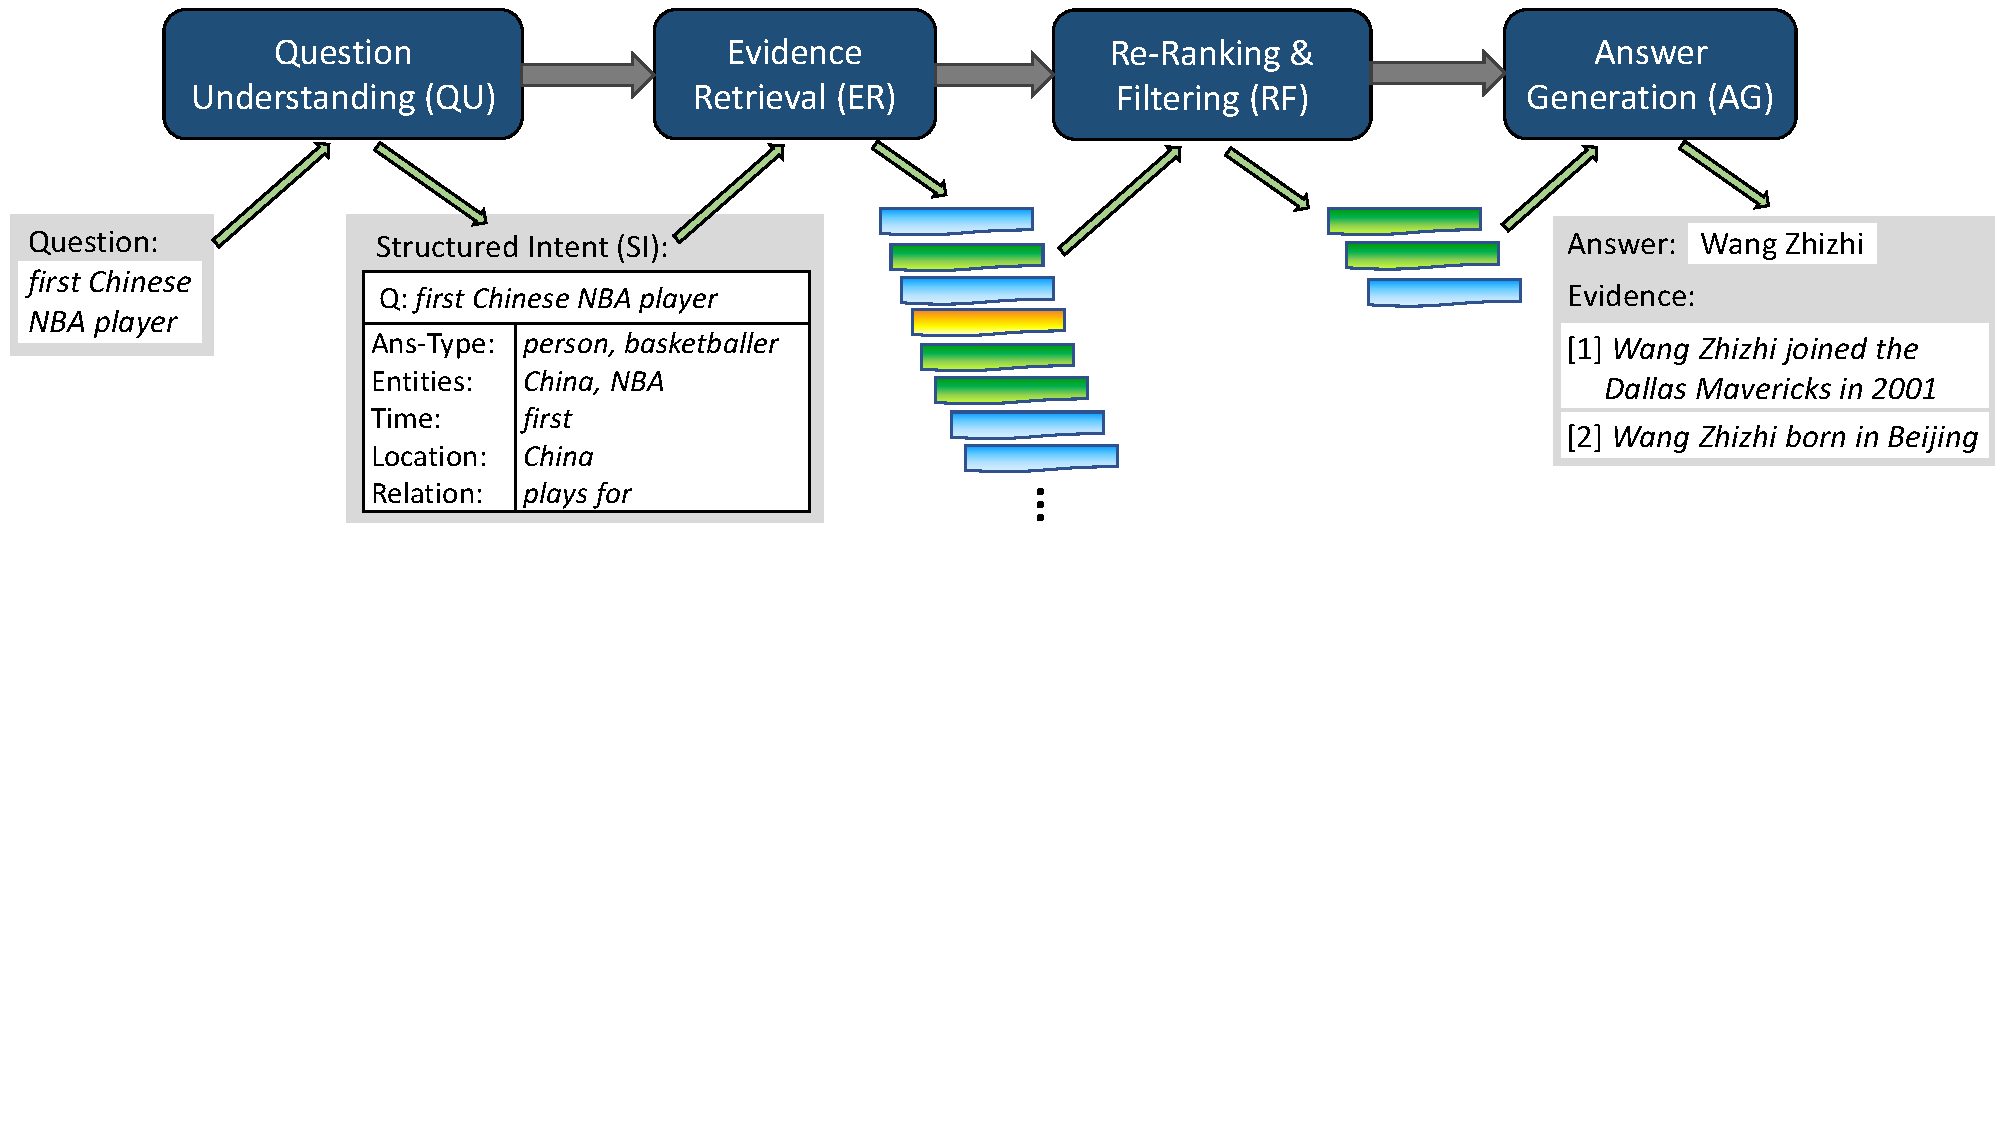
\includegraphics[width=\textwidth]{submissions/Gerhard2024/figures/compass-overview.pdf}
  \caption{Overview of the \method system.}
  \label{fig:compass-overview}
\end{figure}

% start with system overview
The \method system is a pipeline of four major stages, as illustrated in Figure \ref{fig:compass-overview}.
First, the input question is analyzed and decomposed, in order to compute a {\em structured intent (SI)} representation that will pass on to the subsequent steps, along with the original question. Second, the SI is utilized to retrieve pieces of evidence from different sources: text, KG and tables. 
Third, this pool of potentially useful evidence is filtered down, with iterative re-ranking, to arrive at a tractably small set of most promising evidence.
The final stage generates the answer from this evidence,
passing back the answer as well as evidence snippets for user-comprehensible explanation.

The second and fourth stage, Evidence Retrieval (ER) and Answer Generation (AG), are fairly standard. Such a two-phase architecture was called a retriever-reader architecture~\cite{Zhu-ODQA-survey:arxiv2021}. With a modern LLM replacing the earlier kinds of neural readers, this is the core of every RAG system~\cite{DBLP:journals/arXiv/abs-2312-10997}.

Stages 1 and 3 are unique elements of our architecture, judiciously introduced to improve both effectiveness (i.e., answer quality) and efficiency (i.e., computational cost).
Question Understanding (QU) provides the ER component with crisper and semantically refined input, and
the Re-Ranking \& Filtering (RF) stage is beneficial for
distilling the best evidence from the large pool of retrieved pieces.
The following subsections elaborate on the four stages of the pipeline, emphasizing the \method-specific steps QU and RF.



\subsection{Question Understanding (QU)}

% one par introducing the SI
To prepare the retrieval from different kinds of sources, including a KG, ad-hoc tables and text documents, it is useful to analyze and decompose the user question.
In this work, we aim to cast a question into a 
{\em structured intent (SI)} representation: essentially
a frame with faceted cues as slots, or equivalently, a concise set of key-value pairs. 
Figure \ref{fig:compass-overview} gives an idealized example for the question about the first Chinese NBA player. The facets or keys of potential interest here 
are:
\squishlist
\item {\em Ans-Type:} the expected answer type (or types when considering
different levels of semantic refinement), 
\item {\em Entities:} the salient entities in the question, and 
\item {\em Relation:} phrases that indicate which relation (between Q and A entities) the user is interested in. 
\squishend
\noindent In addition, as questions can have temporal or spatial aspects, the SI also foresees slots for:
\squishlist
\item {\em Time:} cues about answer-relevant time points or spans, including relative cues (e.g., ``before Covid'') and ordinal cues (e.g., ``first''), and
\item {\em Location:} cues about answer-relevant geo-locations.
\squishend

% discuss the spectrum of different SIs
\vspace{0.2cm}
\noindent The ideal SI for example question Q2 would look like:

\begin{quote}
{\em Ans-Type:} person, basketballer; {\em Entities:} China, NBA; {\em Time:} first;
{\em Location:} China; {\em Relation:} plays for.
\end{quote}

Note that the values for these slots can be crisp like entity names or dates, but they can also take the form of surface phrases. The SI purpose and value lie in the decomposition. In practice, many questions would only lead to a subset of faceted cues, leaving some slots empty. For the example in Figure \ref{fig:compass-overview}, an alternative SI could simply consist of

\begin{quote}
{\em Ans-Type:} person; {\em Entities:} China, NBA; {\em Time:} first.
\end{quote}

\noindent Even this simplified SI can be highly beneficial in guiding the subsequent evidence retrieval.

% sketch how an LM is trained to generate SIs 
To generate the SI from a user question, we employ a (small-scale) LM, specifically BART~\cite{DBLP:conf/acl/LewisLGGMLSZ20}, a Transformer-based auto-encoder with 140M parameters.\footnote{\url{https://huggingface.co/facebook/bart-base}}
BART is pre-trained for language representation; its power for our purpose comes from fine-tuning.
To this end, we generate (question, SI) pairs by using an instruction-trained LLM like GPT-4, with few-shot in-context learning (following our earlier work~\cite{Jia-FAITH:WWW2024}). 
Note that this is a one-time action; at inference-time we only use much smaller LMs.
The generated silver-standard pairs are then used to fine-tune BART.
In the experiments in this article, we leverage pre-existing collections of silver pairs, based on the training data of the CompMix benchmark~\cite{Christmann-CompMix:WWW2024}, 
comprising $3{,}400$ such pairs.


% outline value of SI for conversations
Although this paper focuses on single-shot questions, the \method architecture is also geared for conversational QA. In that setting, the SI can play an even bigger role, as (follow-up) questions are often formulated in a rather sloppy manner -- all but self-contained. For example, a conversation could start with a clear question {\em When did Wang Zhizhi join the NBA?}, followed a few dialog steps later, by a user utterance like {\em Which teams did he play for?} or simply {\em Which teams?}.
In such an informal conversation, the system needs to {\em contextualize} each user utterance based on the preceding turns in the dialog (e.g., inferring the relevant entities Wang Zhizhi and NBA from the conversational history).
For details on conversational QA, based on our architecture, see our earlier works~\cite{Christmann-CONVINSE:SIGIR2022,Christmann-Explaignn:SIGIR2023}.







%%%%%%%%%%%%%%%%%%%%%%%%%%%%%%%%%%%%%
\subsection{Evidence Retrieval (ER)}

The ER stage taps into a knowledge graph, a corpus of text documents, and a collection of web tables.
Specifically, for the experiments, we use the Wikidata KG,
all English Wikipedia articles, and all tables that are embedded in Wikipedia pages (incl. infoboxes, which can be seen as a special case of tables). 

% specifics: Clocq etc. - and the role of the SI
\vspace{0.2cm}
\noindent{\bf Retrieval from KG:}
To retrieve evidence from the KG, we utilize our earlier work
\clocq~\cite{Christmann-CLOCQ:WSDM2022}, which provides entity disambiguations and a relevant KG-subgraph for a given query.
Unlike most other works on QA-over-KG, \clocq fetches all KG-facts that are relevant for a given entity in a single step.
For example, when querying for
NBA players, it can traverse the KG neighborhood and pick up top teams, also considering so-called qualifier nodes in Wikidata which are often used for temporal scopes. 
As the disambiguation of entity names onto the KG can be tricky and noisy (e.g., China could be mapped to Chinese sports teams in all kinds of sports), \clocq considers several possible disambiguations~\cite{Christmann-CLOCQ:WSDM2022} (typically in the order of $10$ result entities).
The queries for \clocq are 
constructed by concatenating all slots of the question's SI.
For the example query about the first Chinese NBA player,
good result entities would be Dallas Mavericks, lists about NBA seasons, MVP awards etc., and their associated facts. These provide cues, but are likely insufficient to answer the question.


\vspace{0.2cm}
\noindent{\bf Retrieval from Text and Tables:}
The disambiguated entities returned by \clocq form anchors for tapping into text and tables.
\method first identifies 
relevant text documents and tables that refer to the anchor entities. With focus on Wikipedia, these are simply the articles for the respective entities. 
\method then constructs a keyword query that concatenates all available fields of the SI.
The query is evaluated against a linearized and verbalized representation (see below) of all sentences and all table rows in the selected documents.
This returns a set of sentences and 
and individual table rows, ranked by BM25 scores.


\vspace{0.2cm}
\noindent{\bf Evidence Verbalization:}
All results from the different data sources are uniformly treated by {\em linearizing} and {\em verbalizing} them
into token sequences. For KG results, the entity-centric triple sets are linearized via breadth-first traversal of the mini-graph starting from the entity node.
For tables, results are individual rows, which are contextualized by including labels from column headers and from the DOM-tree path of the article where the table comes from. For example, a table row about Wang Zhizhi playing for Dallas (Mavericks) in the 2000-2001 season, would be expressed as:

\vspace{0.05cm}
\hspace*{0.5cm} Wang Zhizhi / NBA Career / Season: 2000-2001, Team: Dallas, Games Played: 5 \dots
\vspace{0.05cm}

\noindent Finally, results from the text corpus are already in the form of token sequences, but we can additionally prefix these with the DOM-tree labels.
We can think of this entire pool of evidence as 
an on-the-fly corpus of potentially relevant pseudo-sentences, forming the input of the subsequent RF stage.


\vspace{0.2cm}
\noindent {\bf Result Ranking:}
Overall, the ER stage compiles a substantial set of evidence, possibly many thousands of entities, text snippets and table rows. Therefore, we practically restrict the pool to a subset of high-scoring pieces, like the top-$1000$.
For scoring, a simple BM25 model (a classical IR method) is applied. 
By default, we treat all evidence pieces uniformly with global scoring, no matter whether they come from KG, text or tables. 


\subsection{Re-Ranking and Filtering (RF)}

With a pool of top-$1000$ evidence pieces, we could invoke an LLM for answer generation. However, that would face a large fraction of noise (i.e., misleading evidence) and incur high costs of computation and energy consumption. 

For both of these reasons, we have devised light-weight techniques for iteratively reducing the top-$1000$ pieces to a small subset, say top-$30$ or top-$10$, that can be fed into an LLM at much lower cost (as LLM computations and pricing are at least linear in the number of input tokens). The difficulty is, of course, to do this without losing good evidence and reducing answer presence. Our techniques for this task are based on graph neural networks (GNNs)~\cite{Wu:IEEE2021} or cross-encoders (CEs)~\cite{Dejean:arxiv2024,Lin:MC2021}.

\myparagraph{GNN-based RF}
Given a large pool of evidence pieces from all sources, a bipartite graph is constructed:
\squishlist
\item {\em nodes} being evidence pieces or entities that occur in these pieces, and
\item {\em edges} connecting an evidence piece and an entity if the entity occurs in the evidence.
\squishend


The task for the GNN is to jointly score the evidence and the entity nodes in a multi-task learning setup. The latter are the {\em answer candidates}, and the evidence should give {\em faithful explanation} for an answer.
We build on our earlier work on explainable QA~\cite{Christmann-Explaignn:SIGIR2023}.

The node encodings are initialized with cross-encoder embeddings (see below) 
for node contents and the SI of the question. The inference iteratively adjusts the encodings based on message passing from neighboring nodes.
The GNN is trained via weak supervision from question-answer pairs:
evidence nodes are labeled as relevant if they are connected to
a gold answer.
More technical details are given in~\cite{Christmann-Explaignn:SIGIR2023}.

\method invokes the GNN in multiple rounds, iteratively reducing top-$k$ to top-$k^*$ nodes with $k^* \ll k$. In practice, we would typically consider two rounds: re-ranking top-$1000$ and pruning to top-100, and then reducing to top-30 or top-10, which are passed to the answer generation stage.
Note that this keeps the GNN at a tightly controlled size, so that its computational costs at inference-time are much smaller than those of an LLM.


\myparagraph{CE-based RF}
An alternative to the GNN inference is to employ a cross-encoder for scoring and re-ranking the evidence pieces.
These are transformers (typically with a small LM like BERT) that are fine-tuned for scoring the relatedness between a query and a document~\cite{Nogueira:arxiv2019}. In our case, the comparison is between the question SI and the evidence piece. In our experiments, we make use of two different cross-encoders, 
both trained on the MS-MARCO benchmark for passage retrieval~\cite{Bajaj:arxiv2018}, 
and fine-tuned on the respective benchmark (leveraging the same weak supervision data as for the GNNs),
the difference being in model size.\footnote{\url{https://huggingface.co/cross-encoder/ms-marco-MiniLM-L-4-v2} and\\ \url{https://huggingface.co/cross-encoder/ms-marco-MiniLM-L-6-v2}}
We use the smaller model to reduce top-$1000$ to top-100, and the larger model to go further down from top-100 to top-30.




%%%%%%%%%%%%%%%%%%%%%%%%%%%%%%%%%%%%%

\subsection{Answer Generation (AG)}

The last stage follows mainstream practice to invoke an LLM in a retrieval-augmented manner.
We call a `small-scale` LLM, specifically a fine-tuned LlaMA-3.1 model (8B-Instruct)\footnote{\url{https://huggingface.co/meta-llama/Llama-3.1-8B-Instruct}}, with a prompt \footnote{The specific prompt is \phrase{SI: \textless\texttt{concatenated SI}\textgreater \hspace{0.1cm} Evidence: \textless\texttt{evidence pieces}\textgreater}.}
consisting of:

\squishlist
\item the concatenated SI of the original question, and
\item the top-30 (or other top-$k^*$ with small $k^*$) evidence pieces.
\squishend

By the previous down-filtering of the original pool of evidence pieces, this last step has affordable cost in terms of computation time and energy consumption.

\vspace{0.2cm}
\noindent{\bf Fine-Tuning the LLM:}
We considered adding an instruction to the prompting, such as {\em ``answer this question solely based on the provided evidence snippets''}.
However, this turned out to be ineffective.
The reason why the model works well without such instructions is our task-specific fine-tuning.
We perform this by running the training data of benchmarks through the \method pipeline,
and training the AG stage with the top-30 evidence pieces as input.
Thus, the fine-tuning makes the model learn the role of evidence for RAG-based QA.

\vspace{0.2cm}
\noindent{\bf Explanations:}
The top-30 evidence pieces can be used to provide users with explanation of answers.
Optionally, these could be reduced further for comprehensibility.
Alternatively, we can fine-tune the LLM to provide both answers and concise explanations.
Since we can infer which evidences in the input mention the annotated ground-truth answers,
our method could be fine-tuned to provide such \textit{answering evidences} as well (cf.~\cite{Gao-citations:emnlp2023}).

\label{sec:exp}
\section{Experiments}


\label{setup}
\subsection{Experimental setup}


%%% BENCHMARKS
\myparagraphnospace{Benchmarks} We run experiments on three benchmarks with different characteristics of questions.

\squishlist
    \item \textbf{\compmix}.
    \compmix~\cite{Christmann-CompMix:WWW2024} is a benchmark which was specifically designed for evaluating QA systems operating over heterogeneous sources. The dataset has $9{,}410$ questions, out of which $2{,}764$ are used for testing.
    Answers are crisp entity names, dates, or other literals.
    
    \item \textbf{\crag}.
    We further evaluate on a subset of the \crag~\cite{Yang-CRAG} dataset, which was recently released as a testbed for RAG-based QA systems.
    We utilize the same pipeline and sources as outlined in Section~\ref{sec:method}, without using the web snippets or APIs provided with \crag. This way we focus on entity-centric questions that do not require access to live web data (e.g., news feeds), and disregard cases where the results would be up-to-date quantities.
    This restricts the test data to $436$ entity-centric questions, still enough for a proof of concept.
    
    \item \textbf{\timequestions}.
    To showcase the generalizability of our pipeline, we conduct experiments on~\timequestions~\cite{Jia-TimeQuestions},
    a benchmark for temporal QA. The dataset requires temporal understanding and reasoning, which are well-known limitations of
    LLMs~\cite{Dhingra-time-aware-LLM:TACL2022}. \timequestions has 16{,}181 questions (3{,}237 for testing).
\squishend

Typical examples for the questions in these three benchmarks are:

\begin{quote}
\compmix: \utterance{Which player won the most number of Man-of-the-Match titles in the FIFA world cup of 2006?}\\
 \indent \crag: \utterance{What was the worldwide box office sales for little hercules?}\\ 
  \indent \timequestions: \utterance{Which club did Cristiano Ronaldo play for before joining Real Madrid?}
\end{quote}

%%% BASELINES
\myparagraph{Baselines} As competitors or reference points to \method, we study the performance of the following methods:

\squishlist
    \item \textbf{Generative LLMs}.
    We compare \method against out-of-the-box LLMs: \textbf{\gptthree} (\texttt{text-davinci-003}), \textbf{\gptfour} (\texttt{gpt-4}) 
    and \textbf{\llama} (\texttt{meta-llama/Llama-3.1-8B-Instruct}).
    The same prompt is used for all LLMs, consistent with previous work~\cite{Christmann-CompMix:WWW2024, Zhang-Spaghetti:ACL2024}:
    \phrase{Please answer the following question by providing the crisp answer entity, date, year, or numeric number. Q: \textless\texttt{question}\textgreater}.
    

    \item \textbf{Heterogeneous QA methods}.
    \convinse~\cite{Christmann-CONVINSE:SIGIR2022}, \unikqa~\cite{Oguz-UniK-QA:NAACL2022}, \explaignn~\cite{Christmann-Explaignn:SIGIR2023}
    are QA methods designed to integrate heterogeneous sources: text, tables and KG. All of these  integrate the exact same sources as \method.

    
    \item \textbf{\textsc{State-of-the-art}}.
    For \compmix and \timequestions, we also compare against state-of-the-art methods from the literature: \spaghetti~\cite{Zhang-Spaghetti:ACL2024} and \textsc{Un-Faith}~\cite{Jia-FAITH:WWW2024}, which are among the best performing systems.
    
Results are taken from the literature whenever applicable.
On \crag, we use the models trained on \compmix for \method and heterogeneous QA baselines.
\squishend



%%% METRIC(S)
\myparagraph{Metrics}
We measure \textit{precision at 1} (\textbf{P@1}) as our main metric~\cite{RoyAnand:MC2021} on all benchmarks.
On \crag, we manually annotate answer correctness, as the ground-truth answer formats vary (e.g., entity name variants, lists, sentences).

We also compute the number of neural parameters aggregated over all sub-modules (\textbf{\#Parameters}).
Parameter counts for GPT-models are taken from~\cite{Minaee-LLM-survey}
(\gptfour might have less active parameters during inference).

For further analysis we measure \textit{answer presence} (\textbf{AP@k}),
i.e. whether the answer is present in the top-$k$ ranked evidence pieces,
and \textit{mean reciprocal rank} within the top-$k$ evidences (\textbf{MRR@k}).

%%% CONFIG
\myparagraph{Configuration}
Our implementation uses the \texttt{Llama3.1-8B-Instruct} model for the AG stage.
For the QU, ER and RF stages
we adopt code from the \explaignn project.\footnote{\url{https://explaignn.mpi-inf.mpg.de}}
For the ER stage, we use \clocq, setting its specific parameters to $k=10$ and $p=1{,}000$.

As default, we use the GNN technique for the RF stage.
For efficiency, we use light-weight models for initializing
the GNN encoders -- the same models used for the CE-based RF.\footnote{\url{https://huggingface.co/cross-encoder/ms-marco-MiniLM-L-4-v2} and\\\url{https://huggingface.co/cross-encoder/ms-marco-MiniLM-L-6-v2}}
The GNNs are trained for $5$ epochs with an epoch-wise evaluation strategy,
i.e. we choose the model with the best performance on the respective dev set.
We train the GNNs on graphs with a maximum of $100$ evidence and $400$ entity nodes (as scored by BM25).
During inference, the first GNN is applied on graphs with $1{,}000$ evidence and $4{,}000$ entity nodes, shrinking the pool of evidence pieces to the top-$100$.
The second GNN then runs on graphs with $100$ evidence and $400$ entity nodes.
The factor of 4 entities per evidence (on average) holds sufficient for the observed data,
and enables batched inference.
Other parameters are kept as is.

The AG model, based on \texttt{Llama3.1-8B-Instruct}, is 
fine-tuned
for $2$ epochs with a warm-up ratio of $0.01$ and a batch size of $8$, again with an epoch-wise evaluation strategy.
Other parameters are set to the default Hugging Face
training parameters.\footnote{\url{https://huggingface.co/docs/transformers/v4.46.2/en/main_classes/trainer\#transformers.TrainingArguments}}





\subsection{Main results}
%%% MAIN TABLE
\myparagraphnospace{\method is competitive on all benchmarks}
Main results of our experiments are shown in Table~\ref{tab:main-res}.
First of all, we note that \method achieves competitive performance across all three benchmarks.

On \compmix, baselines for heterogeneous QA and \llama perform similarly,
whereas GPT-based LLMs can answer more than $50$\% of the questions correctly.
\method exhibits substantially higher performance, on par with
the state-of-the-art method \textsc{Spaghetti}~\cite{Zhang-Spaghetti:ACL2024}
(which is based on \gptfour).

On the \crag dataset, P@1 drops for all methods except for \gptfour. 
The benchmark includes realistic questions,
which can be ambiguous/confusing (\phrase{who was the director for the report?}),
on ``exotic'' entities with answers in social media (\phrase{how many members does the teknoist have?}),
or require up-to-date information (\phrase{when did chris brown release a song or album the last time?}),
and other cases that are challenging for all methods.

Finally, \method establishes new state-of-the-art performance on the \timequestions benchmark.
Interestingly, all of the tested LLMs show greatly reduced performance on this benchmark,
which inherently requires temporal understanding and reasoning
-- a known weakness of stand-alone LLMs.


\begin{table} [h]
    \centering
    \newcolumntype{G}{>{\columncolor [gray] {0.90}}c}
    \begin{tabular}{l G G G c}
        \toprule
            \textbf{Method $\downarrow$ / Benchmark $\rightarrow$} & \textbf{\compmix}  & \textbf{\crag} & \textbf{\timequestions} & \textbf{\#Parameters} \\ 
        \midrule
            \textbf{\gptthree} 
            & $0.502$ &   $-$ & $0.224$ & $175{,}000$ M  \\
            % #params from https://arxiv.org/pdf/2402.06196

            \textbf{\gptfour}
            & $0.528$ &   $\mathbf{0.633}$ & $0.306$ & $1{,}760{,}000$ M \\
            % #params from https://arxiv.org/pdf/2402.06196

            \textbf{\llama~\cite{Touvron-LLaMA}} (8B-Instruct)
            & $0.431$ &   $0.385$ & $0.178$ & $8{,}030$ M  \\
            % #params from Huggingface (8,030,257,152)
        \midrule
            \textbf{\convinse~\cite{Christmann-CONVINSE:SIGIR2022}}
            & $0.407$  &   $0.298$ & $0.423$  & $362$ M \\
            % FiD: 222,903,936 + BART (SR-generation): 139,420,416 = 362,324,352 (python explaignn/question_understanding/structured_representation/get_num_params.py)

            \textbf{\unikqa~\cite{Oguz-UniK-QA:NAACL2022}}
            & $0.440$ &   $0.280$ & $0.424$ & $223$ M  \\
            % FiD: 222,903,936 (python explaignn/heterogeneous_answering/fid_module/FiD/get_num_params.py)
    
            \textbf{\explaignn~\cite{Christmann-Explaignn:SIGIR2023}} 
            & $0.442$ &   $0.303$ & $0.525$  & $328$ M \\
            % BART (SR-generation): 139,420,416 + 2GNNs: 94520832 + 93930240 = 327,871,488

        \midrule 
            \textbf{\textsc{State-of-the-art}}
            & $\mathbf{0.565}$ 
            & $-$
            & $0.571$  & $-$ \\

            & (\textsc{Spaghetti}~\cite{Zhang-Spaghetti:ACL2024})
            & 
            & (\textsc{Un-Faith}~\cite{Jia-FAITH:WWW2024}) &  \\

        \midrule
            \textbf{\method (ours)}
            & ${0.564}$ &   $0.362$ & $\mathbf{0.754}$  & $8{,}218$ M \\
            % BART (SR-generation): 139,420,416 + LLaMA: 8,030,257,152 + GNNs: 25,670,016 + 22,268,928 =  8,217,616,510
        \bottomrule
    \end{tabular} 
    \vspace*{-0.2cm}
    \caption{End-to-end P@1 of \method and baselines on three benchmarks. Results for \gptthree and \gptfour are taken from the literature~\cite{Christmann-CompMix:WWW2024, Jia-FAITH:WWW2024}. \gptthree is not accessible anymore, hence no results on \crag.
    }
    \label{tab:main-res}
\end{table}





%%% ANSWER SOURCES
\myparagraph{Integration of heterogeneous sources is vital}
\method integrates evidence from text, KG and tables into a unified framework.
We aim to better understand how this affects the answering performance of the method.
Table~\ref{tab:sources} shows end-to-end answering performance of \method
with different combinations of the input sources.
The results clearly indicate that all types of sources contribute, with option Text+KG+Tables performing best,
with a large margin over tapping only single source types.

\begin{table} [t] 
    \centering
    \newcolumntype{G}{>{\columncolor [gray] {0.90}}c}
    \newcolumntype{H}{>{\setbox0=\hbox\bgroup}c<{\egroup}@{}}
    	\begin{tabular}{l G G G H H H c c c} 
        \toprule
            \textbf{Benchmark $\rightarrow$}
                & \multicolumn{3}{G}{\textbf{\compmix}} 
                & \multicolumn{3}{H}{\textbf{\crag}}
                & \multicolumn{3}{c}{\textbf{\timequestions}} \\ 
        \midrule
            \textbf{Input sources $\downarrow$ / Metric $\rightarrow$}
                & \textbf{P@1} & \textbf{AP@100}  & \textbf{AP@30}
                & \textbf{P@1} & \textbf{AP@100}  & \textbf{AP@30}
                & \textbf{P@1} & \textbf{AP@100}  & \textbf{AP@30} \\
            \midrule
                \textbf{Text}           &  $0.455$  &  $0.563$  &  $0.531$ &  $?$  &  $?$  &  $?$ &  $0.539$  &  $0.515$  &  $0.487$   \\
                \textbf{KG}             &  $0.481$  &  $0.677$  &  $0.637$ &  $?$  &  $?$  &  $?$ &  $0.724$  &  $0.701$  &  $0.674$   \\
                \textbf{Tables}         &  $0.432$  &  $0.501$  &  $0.482$ &  $?$  &  $?$  &  $?$ &  $0.536$  &  $0.347$  &  $0.328$   \\
            \midrule
                \textbf{Text+KG}        &  $0.537$  &  $0.749$  &  $0.706$ &  $?$  &  $?$  &  $?$ &  $0.745$  &  $\mathbf{0.776}$  &  $0.748$   \\
                \textbf{Text+Tables}    &  $0.503$  &  $0.632$  &  $0.594$ &  $?$  &  $?$  &  $?$ &  $0.567$  &  $0.578$  &  $0.549$   \\
                \textbf{KG+Tables}      &  $0.524$  &  $0.728$  &  $0.692$ &  $?$  &  $?$  &  $?$ &  $ 0.743$  &  $0.731$  &  $0.703$   \\
            \midrule
                \textbf{Text+KG+Tables}    &  $\mathbf{0.564}$  &  $\mathbf{0.759}$  &  $\mathbf{0.724}$ &  $?$ &  $?$  &  $?$ & $\mathbf{0.754}$    & $\mathbf{0.776}$  &  $\mathbf{0.749}$   \\
            \bottomrule
    \end{tabular}
    \vspace*{-0.2cm}
    \caption{Answer presence and answering precision of \method with different combinations of input sources (on the respective test sets).}
    \label{tab:sources}
\end{table}




\subsection{Analysis}

%%% TOP-K vs. 3xTOP-(K/3)
\myparagraph{Unified retrieval enhances performance}
In the RF stage, we re-rank and filter evidence from different source types,
and feed the unified top-\textit{k}* into the AG stage.
We conduct a comparison in which we consider
the top-$10$ evidence pieces from each source type individually. This gives equal influence to KG, text and tables, whereas our default is based on global ranking.
Table~\ref{tab:unified-retrieval} shows the results for this analysis, showing our default choice performs better.
The reason is that different questions require different amounts of evidence from each of the source types.

\begin{table} [t] 
    \centering
    \newcolumntype{G}{>{\columncolor [gray] {0.90}}c}
    \newcolumntype{H}{>{\setbox0=\hbox\bgroup}c<{\egroup}@{}}
    	\begin{tabular}{l G G H H} 
        \toprule
            \textbf{Input evidences $\downarrow$ / Metric $\rightarrow$} & \textbf{P@1} & \textbf{AP@30}  & \textbf{\crag} & \textbf{\timequestions} \\ 
            \midrule
                \textbf{Top-30 Text+KG+Tables (ours)}             &  $\mathbf{0.574}$  &  $\mathbf{0.710}$  &  $-$  &  $-$   \\
                \textbf{Top-10 Text + Top-10 KG + Top-10 Tables}        &  $0.560$    &  $0.709$  &  $-$  &  $-$   \\
            \bottomrule
    \end{tabular}
    \vspace*{-0.2cm}
    \caption{Answer presence and precision
    of \method for different choices of top-30 
    (on \compmix dev set).}
    \label{tab:unified-retrieval}
\end{table}


%%% NUMBER OF EVIDENCES
\myparagraph{\method works well with small amounts of evidence}
We investigate the 
influence of 
the number of evidence pieces
fed into the AG stage, varying it from $5$ to $100$.
Results are shown in Figure~\ref{fig:res-num-evidences}.
As the curve shows, there is a sharp increase in precision as we add evidence up to 30 or 40 pieces, which is around our default of top-30. This indicates that a certain amount of evidence is needed, to overcome the inherent noise and arrive at sufficient answer presence. 
As we increase the amount of evidence further, we observe a saturation effect, and eventually a degration of performance. Too much evidence not only has diminishing returns, but can actually be confusing for the AG stage. This reconfirms our heuristic choice of top-30: enough for good answering while keeping computational costs reasonably low.


\begin{figure}[t]
    \centering
    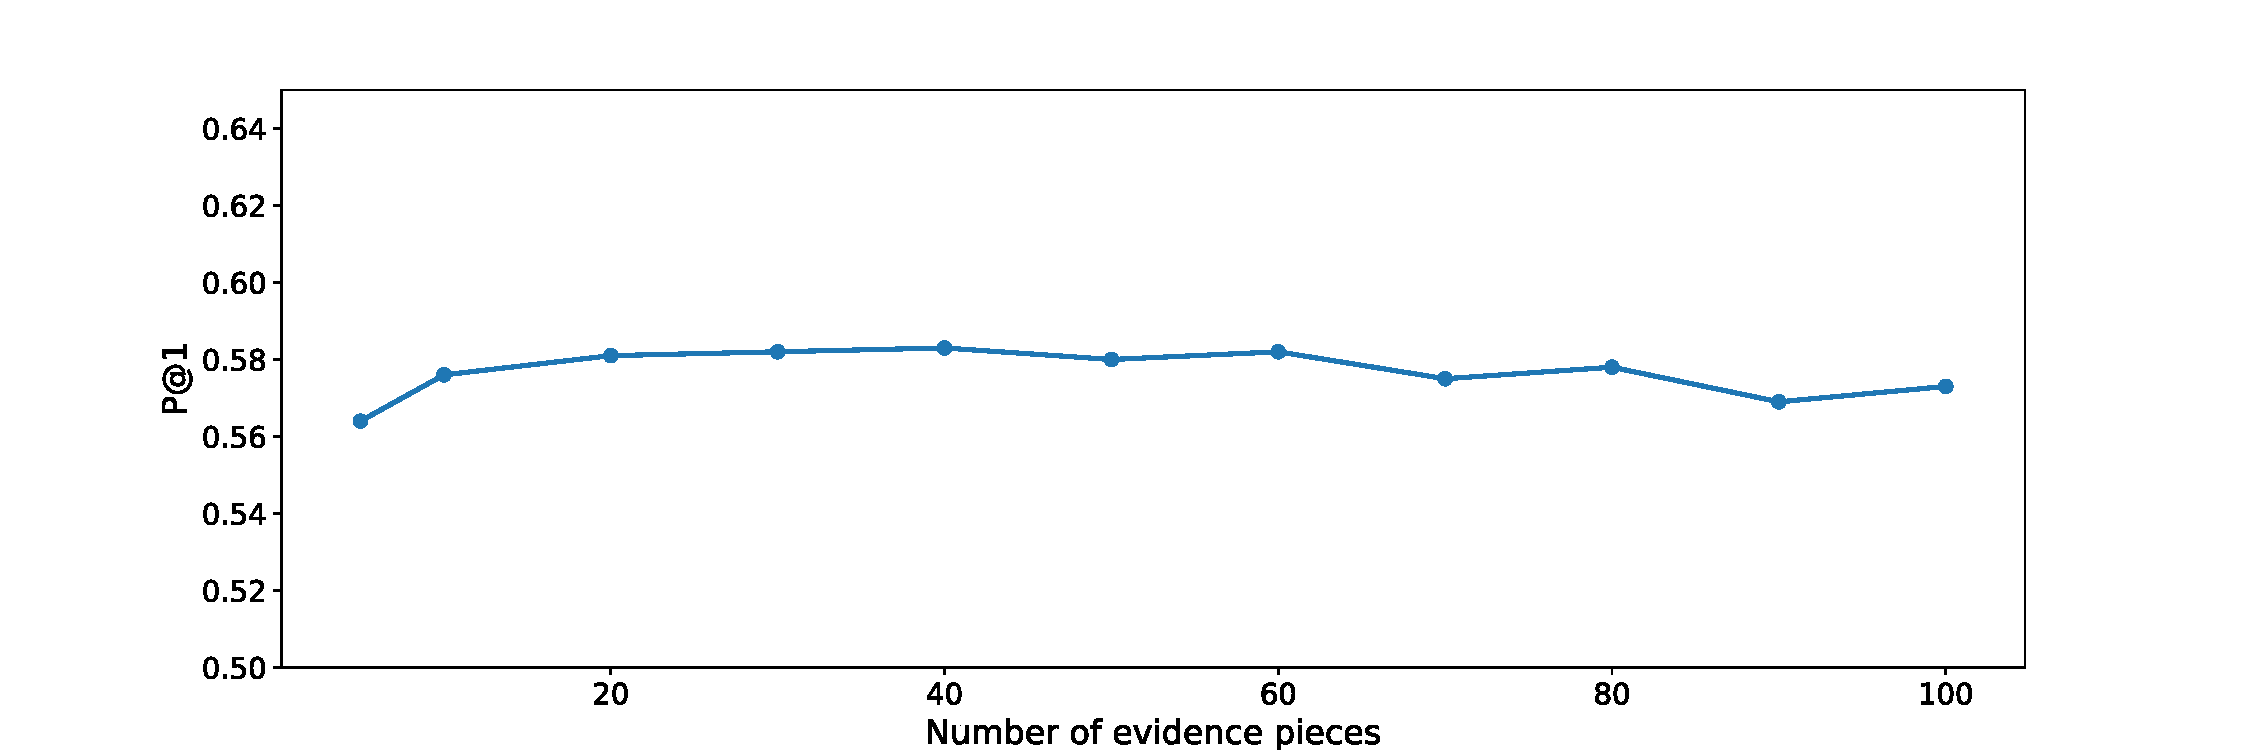
\includegraphics[width=0.8\textwidth]{submissions/Gerhard2024/figures/p_at_1-line_with_evidences.pdf}
    \vspace*{-0.2cm}
    \caption{Performance of \method on the \compmix dev set with different numbers of evidence.}
    \label{fig:res-num-evidences}
    \vspace*{-0.2cm}
\end{figure}



%%% ABLATION
\myparagraph{Ablation study on re-ranking} For more insight on the possible configurations of the RF stage, we conducted an ablation study with different options, including solely relying on the initial BM25 scoring without explicit re-ranking. The results are shown in Table \ref{tab:ablation2}. We observe that the iterative reduction in two steps is slightly better than the single-step variants (going down from top-1000 to top-30 in one RF step). Between the two options of using a GNN or a CE, the differences are negligible. A notable effect is that our RF techniques retain the answer presence at a very high level, only a bit lower than for the initial top-1000. 
The last two rows of Table \ref{tab:ablation2} demonstrate that RF is crucial: without explicit re-ranking, the technique of just picking smaller top-$k$ from the original BM25 model leads to substantial degradation in both answer presence and precision. 


\begin{table} [t] \small
    \centering
    \newcolumntype{G}{>{\columncolor [gray] {0.90}}c}
    \newcolumntype{H}{>{\setbox0=\hbox\bgroup}c<{\egroup}@{}}
    	\begin{tabular}{l G H G G G} 
        \toprule
            & \multicolumn{5}{G}{\textbf{\compmix} (dev set)} \\
        \midrule
            \textbf{RF Method $\downarrow$ / Metric $\rightarrow$} & \textbf{P@1} & \textbf{AP@1000} & \textbf{AP@100}  & \textbf{AP@30} & \textbf{MRR@100} \\ 
        \midrule
            \textbf{GNN: 1000 $\rightarrow$ 100 $\rightarrow$ 30}             &  $\mathbf{0.574}$  & $0.760$ &  $0.738$  &  $0.710$  &  $\mathbf{0.572}$  \\
            \textbf{CE: 1000 $\rightarrow$ 100 $\rightarrow$ 30}          &  $0.573$  & $0.760$  &   $\mathbf{0.740}$ &  $\mathbf{0.721}$   &  $0.553$   \\
        \midrule
            \textbf{GNN: 1000 $\rightarrow$ 30} &  $0.567$  & $?$  &   $n/a$ &  $0.710$   &  $0.567$   \\
         \textbf{CE: 1000 $\rightarrow$ 30} &  $0.570$  & $0.760$  &   $n/a$ &  $0.715$   &  $0.558$   \\
            \midrule
           \textbf{BM25: 100 (w/o GNN or CE)} &  $0.490$ & $0.760$  &  $0.652$  &  $n/a$  &  $0.259$ \\       
            \textbf{BM25: 30 (w/o GNN or CE)} &  $0.468$  & $0.760$  &  $n/a$ &  $0.534$   &  $0.259$   \\
            \bottomrule
    \end{tabular}
    \vspace*{-0.2cm}
    \caption{Ablation study for different RF strategies of \method on the \compmix dev set. The answer presence in the RF input with top-$1000$ evidence pieces is $0.760$.}
    \label{tab:ablation2}
\end{table}



\myparagraph{Quality of SI}
To assess the quality and robustness of the Structured Intents, we
inspected a sample of questions and their SIs.
Table~\ref{tab:question-SI-examples} gives three anecdotic examples.
We show SIs generated by \method, which makes use of the pre-existing collection from the \compmix benchmark for training.
This training data was obtained via different heuristics, 
which can be a limiting factor when user intents become more complex.

Therefore, we also looked at SIs derived via in-context learning (ICL) using \gptfour with $5$ handcrafted examples.
As shown in our earlier work on temporal QA~\cite{Jia-FAITH:WWW2024},
such data can be used for training smaller models (e.g., BART),
which can greatly boost the completeness and overall quality of the generated SIs.

From the sampled set, we observed that the ICL-based SIs are more
complete with all slots filled, whereas the BART-based SIs focused more
on the main slots Answer-type, Entities and Relation.
However, both approaches achieve very high quality in filling the slots,
capturing the user's information need very well.

Interestingly, when questions get complicated, with nested phrases, 
the ICL-based variant succeeds in decomposing the questions, based on only $5$ ICL examples.
For example, for the question {\em ``which German state had the most Corona-related death cases in the first year after the outbreak?''}
the Time slot becomes {\em ``first year after Corona outbreak''},
which can be resolved to identify the temporal scope.
In general, we believe that such question decomposition, beyond simple temporal constraints,
would be an interesting theme for future work.

\begin{table} [t] 
    \centering
    \small
    \newcolumntype{G}{>{\columncolor [gray] {0.90}}c}
    \newcolumntype{H}{>{\setbox0=\hbox\bgroup}c<{\egroup}@{}}
    \resizebox*{\textwidth}{!}{
        \begin{tabular}{p{6cm}|p{6cm}|p{6cm}} 
        \toprule
            \textbf{Question} & \textbf{Current SI by \method} & \textbf{SI via ICL} \\
        \midrule
        \textit{what was disneys first color movie?}
            & Ans-Type: \textit{animated feature film} & Ans-Type: \textit{film, animated film} \\
            & Entities: \textit{disneys} & Entities: \textit{Disney} \\
            & Relation: \textit{was first color movie} & Relation: \textit{first color movie} \\
            &  & Time: \textit{first} \\
        \midrule
        \textit{at the oscars, who won best actor in 2018?}
            & Ans-Type: \textit{human} & Ans-Type: \textit{person, actor} \\
            & Entities: \textit{at the oscars} & Entities: \textit{Oscars, 2018} \\
            & Relation: \textit{who won best actor in 2018} & Relation: \textit{won best actor} \\
            &  & Time: \textit{2018} \\
        \midrule
        \textit{which German state had the most Corona-} & Ans-Type: \textit{state} & Ans-Type: \textit{location, state} \\
        \textit{related death cases in the first year after} & Entities: \textit{Germany, Corona} & Entities: \textit{Germany, Corona-related deaths} \\
        \textit{the outbreak?} & Relation: \textit{which state had the most related} & Relation: \textit{highest count of death cases} \\
        & \textit{death cases in the first year after the out-}  & Location: \textit{Germany} \\
            & \textit{break}  & Time: \textit{first year after Corona outbreak} \\
        \bottomrule
    \end{tabular}
    }
    \vspace*{-0.2cm}
    \caption{Examples for pairs of question and generated SI.}
    \label{tab:question-SI-examples}
\end{table}




%%% REFRAIN FROM ANSWER
\myparagraph{Refraining from answering}
%%% Searched for: "generated_answer I" (with I being the full word, not partial) in the generated answers of LLaMA
%%% yields 245 results out of 2764 questions on CompMix
%%% yields 1270 results out of 3237 questions on TimeQuestions
We can train our model to refrain from answering in scenarios
where the provided evidence does not contain an answer to the question.
Specifically, during training, when the answer is not present in the evidence,
we change the target answer to {\em unknown}. This variant is referred to as \method {\em (faithful)}.

We measure the ratio of questions for which {\em unknown} is provided as answer,
and the P@1 restricted to questions that are answered.
The accuracy of refraining from answering is measured as well,
based on whether the answer is present in the evidence or not.
We conduct this experiment on \compmix and \timequestions,
for which we can compute answer presence exactly.
We also compute results for \llama, which is already instructed 
with the option to answer ``don't know''.
Table~\ref{tab:refrain-from-answer} shows the results.
For \compmix, we observe that \method has high accuracy on refraining when appropriate,
whereas \llama tends to be overconfident with a very small rate of {\em unknowns}, leading to incorrect answers.

\begin{table} [t] \small
    \centering
    \newcolumntype{G}{>{\columncolor [gray] {0.90}}c}
    \newcolumntype{H}{>{\setbox0=\hbox\bgroup}c<{\egroup}@{}}
    	\begin{tabular}{l G G G G c c c c} 
        \toprule
            & \multicolumn{4}{G}{\textbf{\compmix}} & \multicolumn{4}{c}{\textbf{\timequestions}} \\
            \midrule
            \textbf{Metric $\rightarrow$} & \textbf{P@1}  & \textbf{P@1} & \textbf{Refrain} & \textbf{Refrain} & \textbf{P@1}  & \textbf{P@1} & \textbf{Refrain} & \textbf{Refrain} \\ 
            \textbf{Method $\downarrow$} &                 & \textbf{(answered)} & \textbf{rate} & \textbf{accuracy} &                 & \textbf{(answered)} & \textbf{rate} & \textbf{accuracy} \\ 
            \midrule
                \textbf{\llama}             &  $0.431$  &  $0.471$  &  $0.089$  &  $n/a$  &  $0.177$  &  $0.276$  &  $0.392$  &  $n/a$  \\
                \textbf{\method (faithful)}           &  $0.497$  &  $0.713$  &  $0.303$  &  $0.838$ &  $0.597$  &  $0.804$  &  $0.257$  &  $0.864$  \\
            \bottomrule
    \end{tabular}
    \vspace*{-0.2cm}
    \caption{
        Performance of \method with option to refrain from answering (``don't know'').
    }
    \label{tab:refrain-from-answer}
\end{table}

\label{sec:disc}
\section{Insights, Limitations, and Challenges}


\noindent{\bf Benchmark Performance.} Our method, RAG-based \method with an 8B LLaMA model, outperforms much larger LLMs like \gptfour on two of the three benchmarks, with a very large margin for temporal questions. Obviously, pre-trained LLMs have only limited sense of properly positioning ``remembered’’ facts on the timeline even with training data that exceeds ours by several orders of magnitude. This confirms our intuition that LLMs alone are not good at ``recalling’’  higher-arity relations that require combining distant pieces of evidence. This is a sweet spot for RAG. Only for 
the \crag benchmark, \method is substantially inferior to a full-blown LLM. This is likely due to the nature of the questions: not necessarily the complexity of the information needs, but the need for more web sources (beyond what our experiments tap into).

\vspace{0.2cm}
\noindent{\bf Cost/Performance Ratio.} The most important take-away from our experiments is that \method achieves its competitive performance at a much lower cost than the full LLMs. Assuming that the consumed GFlops are proportional to the number of model parameters, \method achieves a cost reduction by a factor of 200x for \gptthree and 2000x for \gptfour. This does not only mean less computation, but also a massively lower electricity bill and climate impact.  

\vspace{0.2cm}
\noindent{\bf Role of Question Understanding.} We did not systematically investigate the influence of the Structured Intent in the \method pipeline. However, the comparison to the big GPT models reflects the role of the SI, as we prompt the GPT models in their natural mode with the original questions. The linearized sequence of available SI slots does not always have major advantages, but there are enough cases where specific facets provide crucial cues. This holds especially for the Entities slot, as this drives the gathering of evidence in the ER stage (cf.~\cite{Christmann-CONVINSE:SIGIR2022}, and for the Time slot, as these cues are often decisive for temporal questions (cf.~\cite{Jia-FAITH:WWW2024}).

\vspace{0.2cm}
\noindent{\bf Role of Re-Ranking.} As our ablation studies show, merely using top-$k$ evidence from an initial BM25-style ranking does not provide good performance. Also, there seems to be sweet spot in the choice of $k$: we need enough evidence for connecting the dots if the question requires multiple pieces of information, or for corroborating candidates if the question finds many useful but noisy pieces. In the experiments, $k=30$ turns out to be good choice; much lower $k$ results in insufficient evidence, and much larger $k$ leads to saturation and ultimately degrading performance. Our argument for iteratively shrinking the candidate set in multiple rounds of re-ranking is substantiated in our experiments, but the gain of doing this, compared to GNN- or CE-based re-ranking from 1000 to 30, is not big. More research is called to better understand the role of ranking in RAG. 

\vspace{0.2cm}
\noindent{\bf Limitations of Evidence Retrieval.}
For ER, we adopted more or less standard techniques. The results showed very good answer presence, in the order of 75\% in the top-100 or even top-30. An important case where this is insufficient are questions that require aggregating information over a large number of evidence pieces. An example is asking for the life-time total of 3-point scores of the basketball player Dirk Nowitzki.
This requires collecting a set of per-season tables with NBA player statistics, but also other web sources with numbers for his career before he joined the NBA (including his youth teams).
Of course, there are sometimes shortcuts like a Wikipedia article or biography mentioning the total number, but this cannot be universally assumed. The bottom line is that ER should be reconsidered as well, striving to improve the recall dimension.

\vspace{0.2cm}
\noindent{\bf Limitations of Answer Generation.}
For AG, we simply rely on a LLM,
using it as an extractor (``reader'') from the given evidence. Despite the wide belief that LLMs can perform deep
reasoning over many pieces of evidence, our experience is that the extraction works only well – robustly and faithfully – for relatively simple questions with a few multi-hop joins or simple aggregation over a few pieces. However, complicated questions such as asking for the top-100 NBA players with the largest number of life-time 3-point scores (again including their pre-NBA careers) are currently out of scope and will likely remain so for quite some time. This offers many opportunities for pushing the envelope further.

\vspace{0.2cm}
\noindent{\bf Trust in Data Sources.}
In our experiments, we considered all heterogeneous sources as trustworthy and unbiased. With focus on Wikidata and Wikipedia, this assumption has been well justified. In the wild, however, input data for RAG-based systems likely exhibit a wide spectrum of quality issues, in terms of stale information, biased positions, or simply false statements. Identifying trustworthy and up-to-date evidence and dealing with conflicting data, has been explored in other contexts (e.g., for KG curation~\cite{Dong-Trust:PVLDB2015}), but remains a major challenge for RAG-based QA.


\vspace{0.2cm}
\noindent{\bf Open Challenges and Future Work.} The best-performing methods in our experiment, mostly \method, reach P@1 values of 56\% for \compmix and 75\% for \timequestions. 
For the latter, the answer presence in the top-100 is only slightly higher; so the AG stage hardly misses anything.
However, for \compmix, the answer presence is 75\% -- much higher than what our system can actually answer. Obviously, closing this gap is a major direction to pursue, with focus on the RF and AG stages. However, missing one fourth of the answers completely in the top-100 pool, is a big problem as well. This requires improving recall at the ER stage, possibly with better guidance by the QU, which in turn needs more sources beyond the scope of our experiments (currently limited to Wikidata and Wikipedia). 

In general, we need to think beyond this kind of ``benchmark mindset’’. Even if we reached 80\% or 90\% precision and recall, we would still have a substantial fraction of questions that are answered incorrectly
or not at all. 
The remaining errors may not be a problem for chatbots, but they would be a showstopper for the deployment of mission-critical applications in business or science. We believe that this big gap is a shortcoming of {\em all methods}, not an issue that comes from the data alone. For trivia-style QA, as looked at in this paper, a smart human in ``open book’’ mode and no time limitation should be able to properly answer practically all questions, just by reading pieces of web contents and putting things together. Neither LLMs nor state-of-the-art RAG are the final solution; substantial research and creative ideas are needed to further advance QA.


\clearpage
\newpage

\newcommand{\bibauthors}[1]{{#1}}
\newcommand{\bibtitle}[1]{\emph{#1}}
\newcommand{\bibconf}[1]{{#1}}

\begin{thebibliography}{10}

\bibitem{Bajaj:arxiv2018}
\bibauthors{Payal Bajaj, Daniel Campos, Nick Craswell, Li Deng, Jianfeng Gao, Xiaodong Liu, Rangan Majumder, Andrew McNamara, Bhaskar Mitra, Tri Nguyen, Mir Rosenberg, Xia Song, Alina Stoica, Saurabh Tiwary, Tong Wang.}
\bibtitle{MS MARCO: A Human Generated MAchine Reading COmprehension Dataset.}
In \bibconf{arXiv 2018}.

\bibitem{DBLP:conf/acl/ChenFWB17}
\bibauthors{Danqi Chen, Adam Fisch, Jason Weston and Antoine Bordes.}
\bibtitle{Reading Wikipedia to Answer Open-Domain Questions.}
In \bibconf{ACL 2017}.

\bibitem{Christmann-CONVINSE:SIGIR2022}
\bibauthors{Philipp Christmann, Rishiraj Saha Roy, Gerhard Weikum.}
\bibtitle{Conversational Question Answering on Heterogeneous Sources.}
In \bibconf{SIGIR 2022}.

\bibitem{Christmann-CLOCQ:WSDM2022}
\bibauthors{Philipp Christmann, Rishiraj Saha Roy, Gerhard Weikum.}
\bibtitle{Beyond NED: Fast and Effective Search Space Reduction for Complex Question Answering over Knowledge Bases.}
In \bibconf{WSDM 2022}.

\bibitem{Christmann-Explaignn:SIGIR2023}
\bibauthors{Philipp Christmann, Rishiraj Saha Roy, Gerhard Weikum.}
\bibtitle{Explainable Conversational Question Answering over Heterogeneous Sources via Iterative Graph Neural Networks.}
In \bibconf{SIGIR 2023}.

\bibitem{Christmann-CompMix:WWW2024}
\bibauthors{Philipp Christmann, Rishiraj Saha Roy, Gerhard Weikum.}
\bibtitle{CompMix: A Benchmark for Heterogeneous Question Answering.}
In \bibconf{WWW 2024}.

\bibitem{Dejean:arxiv2024}
\bibauthors{Herve Dejean, Stephane Clinchant, Thibault Formal.}
\bibtitle{A Thorough Comparison of Cross-Encoders and LLMs for Reranking SPLADE.}
In \bibconf{arXiv 2024}.

\bibitem{Dhingra-time-aware-LLM:TACL2022}
\bibauthors{Bhuwan Dhingra, Jeremy R Cole, Julian Martin Eisenschlos, Daniel Gillick, Jacob Eisenstein, and William W Cohen.}
\bibtitle{Time-Aware Language Models as Temporal Knowledge Bases.}
In \bibconf{TACL 2022}.

\bibitem{Dong-Trust:PVLDB2015}
\bibauthors{Xin Luna Dong, Evgeniy Gabrilovich, Kevin Murphy, Van Dang, Wilko Horn, Camillo Lugaresi, Shaohua Sun, Wei Zhang.}
\bibtitle{Knowledge-Based Trust: Estimating the Trustworthiness of Web Sources.}
In \bibconf{PVLDB 2015}.

\bibitem{DBLP:journals/arXiv/abs-2312-10997}
\bibauthors{Yunfan Gao, Yun Xiong, Xinyu Gao, Kangxiang Jia, Jinliu Pan, Yuxi Bi, Yi Dai, Jiawei Sun, Qianyu Guo, Meng Wang, Haofen Wang.}
\bibtitle{Retrieval-Augmented Generation for Large Language Models: A Survey.}
In \bibconf{arXiv 2023}.

\bibitem{Gao-citations:emnlp2023}
\bibauthors{Tianyu Gao, Howard Yen, Jiatong Yu, Danqi Chen.}
\bibtitle{Enabling Large Language Models to Generate Text with Citations.}
In \bibconf{EMNLP 2023}.

\bibitem{Guu-REALM:ICML2020}
\bibauthors{Kelvin Guu, Kenton Lee, Zora Tung, Panupong Pasupat, Ming-Wei Chang.}
\bibtitle{Retrieval Augmented Language Model Pre-Training.}
In \bibconf{ICML 2020}.

\bibitem{DBLP:conf/eacl/IzacardG21}
\bibauthors{Gautier Izacard, Edouard Grave.}
\bibtitle{Leveraging Passage Retrieval with Generative Models for Open Domain Question Answering.}
In \bibconf{EACL 2021}.

\bibitem{Jia-TimeQuestions}
\bibauthors{Zhen Jia, Soumajit Pramanik, Rishiraj Saha Roy, and Gerhard Weikum.}
\bibtitle{Complex Temporal Question Answering on Knowledge Graphs.}
In \bibconf{CIKM 2021}.

\bibitem{Jia-FAITH:WWW2024}
\bibauthors{Zhen Jia, Philipp Christmann, Gerhard Weikum.}
\bibtitle{Faithful Temporal Question Answering over Heterogeneous Sources.}
In \bibconf{WWW 2024}.

\bibitem{DBLP:journals/arXiv/abs-2305-06984}
\bibauthors{Ehsan Kamalloo, Nouha Dziri, Charles L. A. Clarke, Davood Rafiei.}
\bibtitle{Evaluating Open-Domain Question Answering in the Era of Large Language Models.}
In \bibconf{arXiv 2023}.

\bibitem{Kandpal:ICML2023}
\bibauthors{Nikhil Kandpal, Haikang Deng, Adam Roberts, Eric Wallace, Colin Raffel.}
\bibtitle{Large Language Models Struggle to Learn Long-Tail Knowledge.}
In \bibconf{ICML 2023}.

\bibitem{DBLP:conf/emnlp/KarpukhinOMLWEC20}
\bibauthors{Vladimir Karpukhin, Barlas Oguz, Sewon Min, Patrick S. H. Lewis, Ledell Wu, Sergey Edunov, Danqi Chen, Wen-tau Yih.}
\bibtitle{Dense Passage Retrieval for Open-Domain Question Answering.}
In \bibconf{EMNLP 2020}.

\bibitem{Lee-MATTER:ACL2024}
\bibauthors{Dongkyu Lee, Chandana Satya Prakash, Jack FitzGerald, Jens Lehmann.}
\bibtitle{MATTER: Memory-Augmented Transformer Using Heterogeneous Knowledge Sources.}
In \bibconf{ACL 2024}.

\bibitem{DBLP:conf/acl/LewisLGGMLSZ20}
\bibauthors{Mike Lewis, Yinhan Liu, Naman Goyal, Marjan Ghazvininejad, Abdelrahman Mohamed, Omer Levy, Veselin Stoyanov, Luke Zettlemoyer.}
\bibtitle{BART: Denoising Sequence-to-Sequence Pre-training for Natural Language Generation, Translation, and Comprehension.}
In \bibconf{ACL 2020}.

\bibitem{DBLP:conf/nips/LewisPPPKGKLYR020}
\bibauthors{Patrick S. H. Lewis, Ethan Perez, Aleksandra Piktus, Fabio Petroni, Vladimir Karpukhin, Naman Goyal, Heinrich Küttler, Mike Lewis, Wen-tau Yih, Tim Rocktäschel, Sebastian Riedel, Douwe Kiela.}
\bibtitle{Retrieval-Augmented Generation for Knowledge-Intensive NLP Tasks.}
In \bibconf{NeurIPS 2020}.

\bibitem{Lin:MC2021}
\bibauthors{Jimmy Lin, Rodrigo Frassetto Nogueira, Andrew Yates.}
\bibtitle{Pretrained Transformers for Text Ranking: BERT and Beyond.}
In \bibconf{Morgan \& Claypool Publishers 2021}.

\bibitem{Liu-SUQL:NAACL2024}
\bibauthors{Shicheng Liu, Jialiang Xu, Wesley Tjangnaka, Sina J. Semnani, Chen Jie Yu, Monica Lam.}
\bibtitle{SUQL: Conversational Search over Structured and Unstructured Data with Large Language Models.}
In \bibconf{NAACL-HLT 2024}.

\bibitem{Mavi:FnT2024}
\bibauthors{Vaibhav Mavi, Anubhav Jangra, Adam Jatowt.}
\bibtitle{Multi-hop Question Answering.}
In \bibconf{Foundations and Trends in Information Retrieval 2024}.

\bibitem{Minaee-LLM-survey}
\bibauthors{Shervin Minaee, Tomas Mikolov, Narjes Nikzad, Meysam Chenaghlu, Richard}
\bibtitle{Socher, Xavier Amatriain, and Jianfeng Gao.}
Large Language Models: A Survey.
In \bibconf{arXiv 2024}.

\bibitem{Nogueira:arxiv2019}
\bibauthors{Rodrigo Frassetto Nogueira, Kyunghyun Cho.}
\bibtitle{Passage Re-ranking with BERT.}
In \bibconf{arXiv 2019}.

\bibitem{Oguz-UniK-QA:NAACL2022}
\bibauthors{Barlas Oguz, Xilun Chen, Vladimir Karpukhin, Stan Peshterliev, Dmytro Okhonko, Michael Sejr Schlichtkrull, Sonal Gupta, Yashar Mehdad, Scott Yih.}
\bibtitle{UniK-QA: Unified Representations of Structured and Unstructured Knowledge for Open-Domain Question Answering.}
In \bibconf{NAACL-HLT 2022}.

\bibitem{RogersGA:CS2023}
\bibauthors{Anna Rogers, Matt Gardner, Isabelle Augenstein.}
\bibtitle{QA Dataset Explosion: A Taxonomy of NLP Resources for Question Answering and Reading Comprehension.}
In \bibconf{ACM Computing Surveys 2023}.

\bibitem{RoyAnand:MC2021}
\bibauthors{Rishiraj Saha Roy, Avishek Anand.}
\bibtitle{Question Answering for the Curated Web: Tasks and Methods in QA over Knowledge Bases and Text Collections.}
In \bibconf{Synthesis Lectures on Information Concepts, Retrieval, and Services, Morgan \& Claypool Publishers 2021}.

\bibitem{Pramanik-Uniqorn:JWS2024}
\bibauthors{Soumajit Pramanik, Jesujoba Alabi, Rishiraj Saha Roy, Gerhard Weikum.}
\bibtitle{UNIQORN: Unified Question Answering over RDF Knowledge Graphs and Natural Language Text.}
In \bibconf{Journal of Web Semantics 2024}.

\bibitem{Sun-PullNet:EMNLP2019}
\bibauthors{Haitian Sun, Tania Bedrax-Weiss, William W. Cohen.}
\bibtitle{PullNet: Open Domain Question Answering with Iterative Retrieval on Knowledge Bases and Text.}
In \bibconf{EMNLP/IJCNLP 2019}.

\bibitem{Sun:NAACL2024}
\bibauthors{Kai Sun, Yifan Ethan Xu, Hanwen Zha, Yue Liu, Xin Luna Dong.}
\bibtitle{Head-to-Tail: How Knowledgeable are Large Language Models (LLMs)? A.K.A. Will LLMs Replace Knowledge Graphs?}
In \bibconf{NAACL-HLT 2024}.

\bibitem{Touvron-LLaMA}
\bibauthors{Hugo Touvron, Thibaut Lavril, Gautier Izacard, Xavier Martinet, Marie-Anne Lachaux, Timothée Lacroix, Baptiste Rozière, Naman Goyal, Eric Hambro, Faisal Azhar, Aurelien Rodriguez, Armand Joulin, Edouard Grave, Guillaume Lample.}
\bibtitle{Llama: Open and efficient foundation language models.}
In \bibconf{arXiv 2023}.

\bibitem{Wu-STARK:arxiv2024}
\bibauthors{Shirley Wu, Shiyu Zhao, Michihiro Yasunaga, Kexin Huang, Kaidi Cao, Qian Huang, Vassilis N. Ioannidis, Karthik Subbian, James Zou, Jure Leskovec.}
\bibtitle{STaRK: Benchmarking LLM Retrieval on Textual and Relational Knowledge Bases.}
In \bibconf{arXiv 2024}.

\bibitem{Wu:IEEE2021}
\bibauthors{Zonghan Wu, Shirui Pan, Fengwen Chen, Guodong Long, Chengqi Zhang, Philip S. Yu.}
\bibtitle{A Comprehensive Survey on Graph Neural Networks.}
In \bibconf{IEEE Transactions on Neural Networks and Learning Systems 2021}.

\bibitem{Yang-CRAG}
\bibauthors{Xiao Yang, Kai Sun, Hao Xin, Yushi Sun, Nikita Bhalla, Xiangsen Chen, Sajal Choudhary, Rongze D. Gui, Ziran W. Jiang, Ziyu Jiang, Lingkun Kong, Brian Moran, Jiaqi Wang, Yifan Ethan Xu, An Yan, Chenyu Yang, Eting Yuan, Hanwen Zha, Nan Tang, Lei Chen, Nicolas Scheffer, Yue Liu, Nirav Shah, Rakesh Wanga, Anuj Kumar, Wen-tau Yih, Xin Luna Dong.}
\bibtitle{CRAG -- Comprehensive RAG Benchmark.}
In \bibconf{arXiv 2024}.

\bibitem{Yasunaga:NAACL2021}
\bibauthors{Michihiro Yasunaga, Hongyu Ren, Antoine Bosselut, Percy Liang, Jure Leskovec.}
\bibtitle{QA-GNN: Reasoning with Language Models and Knowledge Graphs for Question Answering.}
In \bibconf{NAACL-HLT 2021}.

\bibitem{Zhang-Spaghetti:ACL2024}
\bibauthors{Heidi C. Zhang, Sina J. Semnani, Farhad Ghassemi, Jialiang Xu, Shicheng Liu, Monica S. Lam.}
\bibtitle{SPAGHETTI: Open-Domain Question Answering from Heterogeneous Data Sources with Retrieval and Semantic Parsing.}
In \bibconf{ACL 2024}.

\bibitem{Zhang:NAACL2024}
\bibauthors{Jiahao Zhang, Haiyang Zhang, Dongmei Zhang, Yong Liu, Shen Huang.}
\bibtitle{End-to-End Beam Retrieval for Multi-Hop Question Answering.}
In \bibconf{NAACL-HLT 2024}.

\bibitem{Zhao-LLMsurvey}
\bibauthors{Wayne Xin Zhao, Kun Zhou, Junyi Li, Tianyi Tang, Xiaolei Wang, Yupeng Hou, Yingqian Min, Beichen Zhang, Junjie Zhang, Zican Dong, Yifan Du, Chen Yang, Yushuo Chen, Zhipeng Chen, Jinhao Jiang, Ruiyang Ren, Yifan Li, Xinyu Tang, Zikang Liu, Peiyu Liu, Jian-Yun Nie, Ji-Rong Wen.}
\bibtitle{A Survey of Large Language Models.}
In \bibconf{arXiv 2023}.

\bibitem{Zhao:arxiv2024}
\bibauthors{Penghao Zhao, Hailin Zhang, Qinhan Yu, Zhengren Wang, Yunteng Geng, Fangcheng Fu, Ling Yang, Wentao Zhang, Bin Cui.}
\bibtitle{Retrieval-Augmented Generation for AI-Generated Content: A Survey.}
In \bibconf{arXiv 2024}.

\bibitem{Zhu-ODQA-survey:arxiv2021}
\bibauthors{Fengbin Zhu, Wenqiang Lei, Chao Wang, Jianming Zheng, Soujanya Poria, Tat-Seng Chua.}
\bibtitle{Retrieving and Reading: A Comprehensive Survey on Open-domain Question Answering.}
In \bibconf{arXiv 2021}.

\end{thebibliography}


\end{document}
 
\end{article}
\end{articlesection}

% put the news items below- there can be multiple news sections
% each with its own title
% news will usually have an author as well as a title,
% e.g. TCDE elections
% news articles are in the same format as letters
% typically, news articles will be stored in a directory called "news"


% \begin{newssection}{Obituary}
% \begin{news}{Obituary for Professor Gio Wiederhold}
% {Kyu-Young Whang and Marianne Winslett}{Distinguished Professor Emeritus, KAIST\\ Research Professor Emerita, UIUC\\ together with Gio’s other former students}
% \documentclass[11pt]{article} 

\usepackage{deauthor,times,graphicx}
%\usepackage{url}
\usepackage{hyperref}

\begin{document}
%Obituary for Professor Gio Wiederhold
%                                                                  December 26, 2022                                                                         
Professor Gio Wiederhold passed away in the early hours of December 26, 2022, aged 86, just 10 weeks after an unexpected diagnosis of stage 4 liver cancer. Gio died at home, surrounded by his family members who had gathered for Christmas, including his wife of 56 years, Voy Wiederhold, and his sons John and Randy.  


Gio was a great scholar, educator, and mentor. His influence on the database field is immense. As a pioneer in the database field, he wrote the influential 1977 textbook Database Design, one of the first in the field and adopted around the world. In his DARPA-supported Knowledge-Base Management Systems project in the early 1980s, Gio pioneered the concept of integrating databases and AI, a topic that is now enjoying a revival. Beginning in the 1970s, Gio also pursued the application of databases to medical informatics, another area just now entering the mainstream. In 1992, Gio introduced the notion of mediators (IEEE Computer) as a way of intelligently integrating information from large-scale heterogeneous sources such as databases, file systems, and repositories, a seminal idea for the nascent field of information integration. Gio continued to innovate after retirement from Stanford, most notably in establishing an approach for valuing software and the intellectual property of multinational firms.


Gio advised 36 PhD students at Stanford. Today, Gio’s academic descendants can be found in companies and universities all over the world, including early students Hector Garcia-Molina (the late Stanford professor), David Shaw (DE Shaw founder), Ramez Elmasri (the late textbook author and UT Arlington professor), Kyu-Young Whang (KAIST professor and Naver founder’s advisor), and Marianne Winslett (UIUC professor). Gio’s many subsequent students continue to lead the database field today. 


An influential mentor, Gio always emphasized the practical aspects of research, encouraging people to develop both theoretical and engineering approaches to solve real-world problems. This outlook stemmed from his many years of experience in computing practice before he joined the Stanford University faculty.


Gio’s service to the professional community includes serving as the third Editor-in-Chief of ACM Transactions on Databases during 1985-1995, during which time he significantly contributed to making the new journal a top one in the field. Together with five colleagues, Gio co-founded the IEEE International Conference on Data Engineering in 1984. Perhaps the first venue to use the term data engineering, the conference was unique in focusing on engineering aspects of database research; today it stands as one of the three top-tier conferences in database research. Gio also served as the conference’s program committee chair, co-chair, and general chair in its early years. During 1991-1994, Gio served as the program manager for DARPA’s Knowledge-based Systems program, which collaborated with NSF to fund innovative new research related to information integration and digital libraries — including the project that led to the creation of Google.


In recognition of his many contributions, Gio received the IEEE Technical Community on Data Engineering’s Service Award in 2016. He was also a Fellow of the ACM, the IEEE, and the American College of Medical Informatics.




The many accomplishments and contributions listed above do not capture the full extent of Gio’s impact and influence on our community, nor his diligence and persistence. As Gio’s former students, we dearly miss him for his warm heart towards his students, colleagues, and friends, and above all, his love and kindness for everyone he knew. We are deeply saddened by Gio’s unexpected death and send our sincerest condolences to his surviving family and friends.  




%-- Kyu-Young Whang, Distinguished Professor Emeritus, KAIST and Marianne Winslett, Research Professor Emerita, University of Illinois at Urbana-Champaign, together with Gio’s other former students
\end{document}

% \end{news}

% \newpage
% \end{newssection}


\begin{callsection}

%  This section will be empty for your version
%
%  Calls for papers section.  Use the callsection environment.
%  Each call for papers is contained in an call environment, where the single
%  required options to \begin{call} is the name of the conference.
% typically calls are stored in a "calls" directory
%
%\begin{call}{name of conference}
%\centerline{\includegraphics[width=\textwidth, bb= 0 0 590 760]{calls/conference-name.pdf}}
%\end{call}
%\begin{call}{ICDE 2019 Conference}
%\centerline{\includegraphics[width=\textwidth, bb= 0 0 610 790] {../Dec-2018/calls/icde19.pdf}}
%\centerline{\includegraphics[width=\textwidth, bb= 0 0 590 760] {calls/icde19.pdf}}
%\end{call}
\begin{call}{TCDE Membership Form}
%\centerline{\includegraphics[width=\textwidth, bb= 0 0 610 790]
%\centerline{
\includegraphics[width=\textwidth, bb= 0 0 590 760] {../Dec-2018/calls/tcde.pdf}}
\centerline{
\includegraphics[width=\textwidth, bb= 0 0 590 760] {./calls/tcde.pdf}}
\end{call}

\end{callsection}

\end{bulletin}
\end{document}
